% Options for packages loaded elsewhere
\PassOptionsToPackage{unicode}{hyperref}
\PassOptionsToPackage{hyphens}{url}
\PassOptionsToPackage{dvipsnames,svgnames,x11names}{xcolor}
%
\documentclass[
  letterpaper,
  DIV=11,
  numbers=noendperiod]{scrreprt}

\usepackage{amsmath,amssymb}
\usepackage{iftex}
\ifPDFTeX
  \usepackage[T1]{fontenc}
  \usepackage[utf8]{inputenc}
  \usepackage{textcomp} % provide euro and other symbols
\else % if luatex or xetex
  \usepackage{unicode-math}
  \defaultfontfeatures{Scale=MatchLowercase}
  \defaultfontfeatures[\rmfamily]{Ligatures=TeX,Scale=1}
\fi
\usepackage{lmodern}
\ifPDFTeX\else  
    % xetex/luatex font selection
\fi
% Use upquote if available, for straight quotes in verbatim environments
\IfFileExists{upquote.sty}{\usepackage{upquote}}{}
\IfFileExists{microtype.sty}{% use microtype if available
  \usepackage[]{microtype}
  \UseMicrotypeSet[protrusion]{basicmath} % disable protrusion for tt fonts
}{}
\makeatletter
\@ifundefined{KOMAClassName}{% if non-KOMA class
  \IfFileExists{parskip.sty}{%
    \usepackage{parskip}
  }{% else
    \setlength{\parindent}{0pt}
    \setlength{\parskip}{6pt plus 2pt minus 1pt}}
}{% if KOMA class
  \KOMAoptions{parskip=half}}
\makeatother
\usepackage{xcolor}
\setlength{\emergencystretch}{3em} % prevent overfull lines
\setcounter{secnumdepth}{5}
% Make \paragraph and \subparagraph free-standing
\makeatletter
\ifx\paragraph\undefined\else
  \let\oldparagraph\paragraph
  \renewcommand{\paragraph}{
    \@ifstar
      \xxxParagraphStar
      \xxxParagraphNoStar
  }
  \newcommand{\xxxParagraphStar}[1]{\oldparagraph*{#1}\mbox{}}
  \newcommand{\xxxParagraphNoStar}[1]{\oldparagraph{#1}\mbox{}}
\fi
\ifx\subparagraph\undefined\else
  \let\oldsubparagraph\subparagraph
  \renewcommand{\subparagraph}{
    \@ifstar
      \xxxSubParagraphStar
      \xxxSubParagraphNoStar
  }
  \newcommand{\xxxSubParagraphStar}[1]{\oldsubparagraph*{#1}\mbox{}}
  \newcommand{\xxxSubParagraphNoStar}[1]{\oldsubparagraph{#1}\mbox{}}
\fi
\makeatother

\usepackage{color}
\usepackage{fancyvrb}
\newcommand{\VerbBar}{|}
\newcommand{\VERB}{\Verb[commandchars=\\\{\}]}
\DefineVerbatimEnvironment{Highlighting}{Verbatim}{commandchars=\\\{\}}
% Add ',fontsize=\small' for more characters per line
\usepackage{framed}
\definecolor{shadecolor}{RGB}{241,243,245}
\newenvironment{Shaded}{\begin{snugshade}}{\end{snugshade}}
\newcommand{\AlertTok}[1]{\textcolor[rgb]{0.68,0.00,0.00}{#1}}
\newcommand{\AnnotationTok}[1]{\textcolor[rgb]{0.37,0.37,0.37}{#1}}
\newcommand{\AttributeTok}[1]{\textcolor[rgb]{0.40,0.45,0.13}{#1}}
\newcommand{\BaseNTok}[1]{\textcolor[rgb]{0.68,0.00,0.00}{#1}}
\newcommand{\BuiltInTok}[1]{\textcolor[rgb]{0.00,0.23,0.31}{#1}}
\newcommand{\CharTok}[1]{\textcolor[rgb]{0.13,0.47,0.30}{#1}}
\newcommand{\CommentTok}[1]{\textcolor[rgb]{0.37,0.37,0.37}{#1}}
\newcommand{\CommentVarTok}[1]{\textcolor[rgb]{0.37,0.37,0.37}{\textit{#1}}}
\newcommand{\ConstantTok}[1]{\textcolor[rgb]{0.56,0.35,0.01}{#1}}
\newcommand{\ControlFlowTok}[1]{\textcolor[rgb]{0.00,0.23,0.31}{\textbf{#1}}}
\newcommand{\DataTypeTok}[1]{\textcolor[rgb]{0.68,0.00,0.00}{#1}}
\newcommand{\DecValTok}[1]{\textcolor[rgb]{0.68,0.00,0.00}{#1}}
\newcommand{\DocumentationTok}[1]{\textcolor[rgb]{0.37,0.37,0.37}{\textit{#1}}}
\newcommand{\ErrorTok}[1]{\textcolor[rgb]{0.68,0.00,0.00}{#1}}
\newcommand{\ExtensionTok}[1]{\textcolor[rgb]{0.00,0.23,0.31}{#1}}
\newcommand{\FloatTok}[1]{\textcolor[rgb]{0.68,0.00,0.00}{#1}}
\newcommand{\FunctionTok}[1]{\textcolor[rgb]{0.28,0.35,0.67}{#1}}
\newcommand{\ImportTok}[1]{\textcolor[rgb]{0.00,0.46,0.62}{#1}}
\newcommand{\InformationTok}[1]{\textcolor[rgb]{0.37,0.37,0.37}{#1}}
\newcommand{\KeywordTok}[1]{\textcolor[rgb]{0.00,0.23,0.31}{\textbf{#1}}}
\newcommand{\NormalTok}[1]{\textcolor[rgb]{0.00,0.23,0.31}{#1}}
\newcommand{\OperatorTok}[1]{\textcolor[rgb]{0.37,0.37,0.37}{#1}}
\newcommand{\OtherTok}[1]{\textcolor[rgb]{0.00,0.23,0.31}{#1}}
\newcommand{\PreprocessorTok}[1]{\textcolor[rgb]{0.68,0.00,0.00}{#1}}
\newcommand{\RegionMarkerTok}[1]{\textcolor[rgb]{0.00,0.23,0.31}{#1}}
\newcommand{\SpecialCharTok}[1]{\textcolor[rgb]{0.37,0.37,0.37}{#1}}
\newcommand{\SpecialStringTok}[1]{\textcolor[rgb]{0.13,0.47,0.30}{#1}}
\newcommand{\StringTok}[1]{\textcolor[rgb]{0.13,0.47,0.30}{#1}}
\newcommand{\VariableTok}[1]{\textcolor[rgb]{0.07,0.07,0.07}{#1}}
\newcommand{\VerbatimStringTok}[1]{\textcolor[rgb]{0.13,0.47,0.30}{#1}}
\newcommand{\WarningTok}[1]{\textcolor[rgb]{0.37,0.37,0.37}{\textit{#1}}}

\providecommand{\tightlist}{%
  \setlength{\itemsep}{0pt}\setlength{\parskip}{0pt}}\usepackage{longtable,booktabs,array}
\usepackage{calc} % for calculating minipage widths
% Correct order of tables after \paragraph or \subparagraph
\usepackage{etoolbox}
\makeatletter
\patchcmd\longtable{\par}{\if@noskipsec\mbox{}\fi\par}{}{}
\makeatother
% Allow footnotes in longtable head/foot
\IfFileExists{footnotehyper.sty}{\usepackage{footnotehyper}}{\usepackage{footnote}}
\makesavenoteenv{longtable}
\usepackage{graphicx}
\makeatletter
\newsavebox\pandoc@box
\newcommand*\pandocbounded[1]{% scales image to fit in text height/width
  \sbox\pandoc@box{#1}%
  \Gscale@div\@tempa{\textheight}{\dimexpr\ht\pandoc@box+\dp\pandoc@box\relax}%
  \Gscale@div\@tempb{\linewidth}{\wd\pandoc@box}%
  \ifdim\@tempb\p@<\@tempa\p@\let\@tempa\@tempb\fi% select the smaller of both
  \ifdim\@tempa\p@<\p@\scalebox{\@tempa}{\usebox\pandoc@box}%
  \else\usebox{\pandoc@box}%
  \fi%
}
% Set default figure placement to htbp
\def\fps@figure{htbp}
\makeatother

\KOMAoption{captions}{tableheading}
\makeatletter
\@ifpackageloaded{bookmark}{}{\usepackage{bookmark}}
\makeatother
\makeatletter
\@ifpackageloaded{caption}{}{\usepackage{caption}}
\AtBeginDocument{%
\ifdefined\contentsname
  \renewcommand*\contentsname{Table of contents}
\else
  \newcommand\contentsname{Table of contents}
\fi
\ifdefined\listfigurename
  \renewcommand*\listfigurename{List of Figures}
\else
  \newcommand\listfigurename{List of Figures}
\fi
\ifdefined\listtablename
  \renewcommand*\listtablename{List of Tables}
\else
  \newcommand\listtablename{List of Tables}
\fi
\ifdefined\figurename
  \renewcommand*\figurename{Figure}
\else
  \newcommand\figurename{Figure}
\fi
\ifdefined\tablename
  \renewcommand*\tablename{Table}
\else
  \newcommand\tablename{Table}
\fi
}
\@ifpackageloaded{float}{}{\usepackage{float}}
\floatstyle{ruled}
\@ifundefined{c@chapter}{\newfloat{codelisting}{h}{lop}}{\newfloat{codelisting}{h}{lop}[chapter]}
\floatname{codelisting}{Listing}
\newcommand*\listoflistings{\listof{codelisting}{List of Listings}}
\makeatother
\makeatletter
\makeatother
\makeatletter
\@ifpackageloaded{caption}{}{\usepackage{caption}}
\@ifpackageloaded{subcaption}{}{\usepackage{subcaption}}
\makeatother

\usepackage{bookmark}

\IfFileExists{xurl.sty}{\usepackage{xurl}}{} % add URL line breaks if available
\urlstyle{same} % disable monospaced font for URLs
\hypersetup{
  pdftitle={Data Science II with python (Class notes)},
  colorlinks=true,
  linkcolor={blue},
  filecolor={Maroon},
  citecolor={Blue},
  urlcolor={Blue},
  pdfcreator={LaTeX via pandoc}}


\title{Data Science II with python (Class notes)}
\usepackage{etoolbox}
\makeatletter
\providecommand{\subtitle}[1]{% add subtitle to \maketitle
  \apptocmd{\@title}{\par {\large #1 \par}}{}{}
}
\makeatother
\subtitle{STAT 303-2-Sec20\&21}
\author{}
\date{2025-01-07}

\begin{document}
\maketitle

\renewcommand*\contentsname{Table of contents}
{
\hypersetup{linkcolor=}
\setcounter{tocdepth}{2}
\tableofcontents
}

\bookmarksetup{startatroot}

\chapter*{Preface}\label{preface}
\addcontentsline{toc}{chapter}{Preface}

\markboth{Preface}{Preface}

These are class notes for the course STAT303-2-Sec20\&Sec21 in Winter
2025. This is not the course text-book. You are required to read the
relevant sections of the book as mentioned on the course website.

This book serves as the course notes for {[}Course Name{]}, and it is an
evolving resource developed to support the learning objectives of the
course. It builds upon the foundational work of the original iteration,
authored and maintained by Professor Arvind Krishna. We are deeply
grateful for Professor Krishna's contributions, as his work has provided
a robust framework and valuable content upon which this version of the
book is based.

As the course progresses during this quarter, the notes will be
continually updated and refined to reflect the content taught in real
time. The modifications aim to enhance the clarity, depth, and relevance
of the material to better align with the current teaching objectives and
methodologies.

This book is a living document, and we welcome feedback, suggestions,
and contributions from students, instructors, and the broader academic
community to help improve its quality and utility.

Thank you for being part of this journey, and we hope this resource
serves as a helpful guide throughout the course.

\bookmarksetup{startatroot}

\chapter{Simple Linear Regression}\label{simple-linear-regression}

\emph{Read section 3.1 of the book before using these notes.}

\emph{Note that in this course, lecture notes are not sufficient, you
must read the book for better understanding. Lecture notes are just
implementing the concepts of the book on a dataset, but not explaining
the concepts elaborately.}

\section{Simple Linear Regression}\label{simple-linear-regression-1}

\begin{Shaded}
\begin{Highlighting}[]
\ImportTok{import}\NormalTok{ pandas }\ImportTok{as}\NormalTok{ pd}
\ImportTok{import}\NormalTok{ numpy }\ImportTok{as}\NormalTok{ np}
\ImportTok{import}\NormalTok{ statsmodels.formula.api }\ImportTok{as}\NormalTok{ smf}
\ImportTok{import}\NormalTok{ statsmodels.api }\ImportTok{as}\NormalTok{ sm}
\ImportTok{import}\NormalTok{ seaborn }\ImportTok{as}\NormalTok{ sns}
\ImportTok{import}\NormalTok{ matplotlib.pyplot }\ImportTok{as}\NormalTok{ plt}
\ImportTok{from}\NormalTok{ matplotlib.patches }\ImportTok{import}\NormalTok{ Patch}
\ImportTok{from}\NormalTok{ matplotlib.lines }\ImportTok{import}\NormalTok{ Line2D}
\ImportTok{from}\NormalTok{ sklearn.linear\_model }\ImportTok{import}\NormalTok{ LinearRegression}
\ImportTok{from}\NormalTok{ sklearn.metrics }\ImportTok{import}\NormalTok{ mean\_squared\_error, mean\_absolute\_error, r2\_score}
\end{Highlighting}
\end{Shaded}

\textbf{Develop a simple linear regression model that predicts car price
based on engine size.} Datasets to be used:
\emph{Car\_features\_train.csv, Car\_prices\_train.csv}

\begin{Shaded}
\begin{Highlighting}[]
\CommentTok{\# We are reading training data ONLY at this point.}
\CommentTok{\# Test data is already separated in another file}
\NormalTok{trainf }\OperatorTok{=}\NormalTok{ pd.read\_csv(}\StringTok{\textquotesingle{}./Datasets/Car\_features\_train.csv\textquotesingle{}}\NormalTok{) }\CommentTok{\# Predictors}
\NormalTok{trainp }\OperatorTok{=}\NormalTok{ pd.read\_csv(}\StringTok{\textquotesingle{}./Datasets/Car\_prices\_train.csv\textquotesingle{}}\NormalTok{) }\CommentTok{\# Response}
\NormalTok{train }\OperatorTok{=}\NormalTok{ pd.merge(trainf,trainp)}
\NormalTok{train.head()}
\end{Highlighting}
\end{Shaded}

\begin{longtable}[]{@{}llllllllllll@{}}
\toprule\noalign{}
& carID & brand & model & year & transmission & mileage & fuelType & tax
& mpg & engineSize & price \\
\midrule\noalign{}
\endhead
\bottomrule\noalign{}
\endlastfoot
0 & 18473 & bmw & 6 Series & 2020 & Semi-Auto & 11 & Diesel & 145 &
53.3282 & 3.0 & 37980 \\
1 & 15064 & bmw & 6 Series & 2019 & Semi-Auto & 10813 & Diesel & 145 &
53.0430 & 3.0 & 33980 \\
2 & 18268 & bmw & 6 Series & 2020 & Semi-Auto & 6 & Diesel & 145 &
53.4379 & 3.0 & 36850 \\
3 & 18480 & bmw & 6 Series & 2017 & Semi-Auto & 18895 & Diesel & 145 &
51.5140 & 3.0 & 25998 \\
4 & 18492 & bmw & 6 Series & 2015 & Automatic & 62953 & Diesel & 160 &
51.4903 & 3.0 & 18990 \\
\end{longtable}

\subsection{\texorpdfstring{Training with
\href{https://www.statsmodels.org/stable/index.html}{\texttt{statsmodels}}}{Training with statsmodels}}\label{training-with-statsmodels}

Here, we will use the \texttt{statsmodels.formula.api} module of the
\texttt{statsmodels} library. The use of ``API'' here doesn't refer to a
traditional external web API but rather an interface within the library
for users to interact with and perform specific tasks. The
\texttt{statsmodels.formula.api} module provides a formulaic interface
to the \texttt{statsmodels} library. A formula is a compact way to
specify statistical models using a formula language. This module allows
users to define statistical models using formulas similar to those used
in R.

So, in summary, the \texttt{statsmodels.formula.api} module provides a
formulaic interface as part of the \texttt{statsmodels} library,
allowing users to specify statistical models using a convenient and
concise formula syntax.

\begin{Shaded}
\begin{Highlighting}[]
\CommentTok{\# Let\textquotesingle{}s create the model}
    
\CommentTok{\# ols stands for Ordinary Least Squares {-} the name of the algorithm that optimizes Linear Regression models}

\CommentTok{\# data input needs the dataframe that has the predictor and the response}
\CommentTok{\# formula input needs to:}
    \CommentTok{\# be a string}
    \CommentTok{\# have the following syntax: "response\textasciitilde{}predictor"}
    
\CommentTok{\# Using engineSize to predict price}
\NormalTok{ols\_object }\OperatorTok{=}\NormalTok{ smf.ols(formula }\OperatorTok{=} \StringTok{\textquotesingle{}price\textasciitilde{}engineSize\textquotesingle{}}\NormalTok{, data }\OperatorTok{=}\NormalTok{ train)}
\end{Highlighting}
\end{Shaded}

\begin{Shaded}
\begin{Highlighting}[]
\CommentTok{\#Using the fit() function of the \textquotesingle{}ols\textquotesingle{} class to fit the model, i.e., train the model}
\NormalTok{model }\OperatorTok{=}\NormalTok{ ols\_object.fit()}
\end{Highlighting}
\end{Shaded}

\begin{Shaded}
\begin{Highlighting}[]
\CommentTok{\#Printing model summary which contains among other things, the model coefficients}
\NormalTok{model.summary()}
\end{Highlighting}
\end{Shaded}

\begin{center}
\begin{tabular}{lclc}
\toprule
\textbf{Dep. Variable:}    &      price       & \textbf{  R-squared:         } &     0.390   \\
\textbf{Model:}            &       OLS        & \textbf{  Adj. R-squared:    } &     0.390   \\
\textbf{Method:}           &  Least Squares   & \textbf{  F-statistic:       } &     3177.   \\
\textbf{Date:}             & Tue, 16 Jan 2024 & \textbf{  Prob (F-statistic):} &     0.00    \\
\textbf{Time:}             &     16:46:33     & \textbf{  Log-Likelihood:    } &   -53949.   \\
\textbf{No. Observations:} &        4960      & \textbf{  AIC:               } & 1.079e+05   \\
\textbf{Df Residuals:}     &        4958      & \textbf{  BIC:               } & 1.079e+05   \\
\textbf{Df Model:}         &           1      & \textbf{                     } &             \\
\textbf{Covariance Type:}  &    nonrobust     & \textbf{                     } &             \\
\bottomrule
\end{tabular}
\begin{tabular}{lcccccc}
                    & \textbf{coef} & \textbf{std err} & \textbf{t} & \textbf{P$> |$t$|$} & \textbf{[0.025} & \textbf{0.975]}  \\
\midrule
\textbf{Intercept}  &   -4122.0357  &      522.260     &    -7.893  &         0.000        &    -5145.896    &    -3098.176     \\
\textbf{engineSize} &    1.299e+04  &      230.450     &    56.361  &         0.000        &     1.25e+04    &     1.34e+04     \\
\bottomrule
\end{tabular}
\begin{tabular}{lclc}
\textbf{Omnibus:}       & 1271.986 & \textbf{  Durbin-Watson:     } &    0.517  \\
\textbf{Prob(Omnibus):} &   0.000  & \textbf{  Jarque-Bera (JB):  } & 6490.719  \\
\textbf{Skew:}          &   1.137  & \textbf{  Prob(JB):          } &     0.00  \\
\textbf{Kurtosis:}      &   8.122  & \textbf{  Cond. No.          } &     7.64  \\
\bottomrule
\end{tabular}
%\caption{OLS Regression Results}
\end{center}

Notes: \newline
 [1] Standard Errors assume that the covariance matrix of the errors is correctly specified.

The model equation is: \(\hat{price}\) = -4122.0357 + 12990 *
\texttt{engineSize}

\begin{itemize}
\tightlist
\item
  R-squared is 39\%. This is the proportion of variance in car price
  explained by \texttt{engineSize}.
\item
  The coef of \texttt{engineSize} (\(\hat{\beta}_1\)) is statistically
  significant (\(p\)-value = 0). There is a linear relationship between
  X and Y.
\item
  The 95\% CI of \(\hat{\beta}_1\) is {[}1.25e+04, 1.34e+04{]}.
\item
  PI is not shown here.
\end{itemize}

The coefficient of \texttt{engineSize} is 1.299e+04. - Unit change in
\texttt{engineSize} increases the expected price by \(\$\) 12,990. - An
increase of 3 increases the price by \(\$\) (3*1.299e+04) = \(\$\)
38,970.

The coefficients can also be returned directly usign the \texttt{params}
attribute of the \texttt{model} object returned by the \texttt{fit()}
method of the \texttt{ols} class:

\begin{Shaded}
\begin{Highlighting}[]
\NormalTok{model.params}
\end{Highlighting}
\end{Shaded}

\begin{verbatim}
Intercept     -4122.035744
engineSize    12988.281021
dtype: float64
\end{verbatim}

\textbf{Visualize the regression line}

\begin{Shaded}
\begin{Highlighting}[]
\NormalTok{sns.}\BuiltInTok{set}\NormalTok{(font\_scale}\OperatorTok{=}\FloatTok{1.25}\NormalTok{)}
\NormalTok{ax }\OperatorTok{=}\NormalTok{ sns.scatterplot(x }\OperatorTok{=}\NormalTok{ train.engineSize, y }\OperatorTok{=}\NormalTok{ train.price,color }\OperatorTok{=} \StringTok{\textquotesingle{}orange\textquotesingle{}}\NormalTok{)}
\NormalTok{sns.lineplot(x }\OperatorTok{=}\NormalTok{ train.engineSize, y }\OperatorTok{=}\NormalTok{ model.fittedvalues,color }\OperatorTok{=} \StringTok{\textquotesingle{}blue\textquotesingle{}}\NormalTok{)}
\NormalTok{plt.xlim(}\OperatorTok{{-}}\DecValTok{1}\NormalTok{,}\DecValTok{7}\NormalTok{)}
\NormalTok{plt.xlabel(}\StringTok{\textquotesingle{}Engine size (in litres)\textquotesingle{}}\NormalTok{)}
\NormalTok{plt.ylabel(}\StringTok{\textquotesingle{}Car price\textquotesingle{}}\NormalTok{)}
\NormalTok{legend\_elements }\OperatorTok{=}\NormalTok{ [Line2D([}\DecValTok{0}\NormalTok{], [}\DecValTok{0}\NormalTok{], color}\OperatorTok{=}\StringTok{\textquotesingle{}blue\textquotesingle{}}\NormalTok{, lw}\OperatorTok{=}\DecValTok{4}\NormalTok{, label}\OperatorTok{=}\StringTok{\textquotesingle{}Predicted (Model)\textquotesingle{}}\NormalTok{),}
\NormalTok{                   Line2D([}\DecValTok{0}\NormalTok{], [}\DecValTok{0}\NormalTok{], marker}\OperatorTok{=}\StringTok{\textquotesingle{}o\textquotesingle{}}\NormalTok{, color}\OperatorTok{=}\StringTok{\textquotesingle{}w\textquotesingle{}}\NormalTok{, label}\OperatorTok{=}\StringTok{\textquotesingle{}Actual\textquotesingle{}}\NormalTok{,}
\NormalTok{                          markerfacecolor}\OperatorTok{=}\StringTok{\textquotesingle{}orange\textquotesingle{}}\NormalTok{, markersize}\OperatorTok{=}\DecValTok{10}\NormalTok{)]}
\NormalTok{ax.legend(handles}\OperatorTok{=}\NormalTok{legend\_elements, loc}\OperatorTok{=}\StringTok{\textquotesingle{}upper left\textquotesingle{}}\NormalTok{)}\OperatorTok{;}
\end{Highlighting}
\end{Shaded}

\pandocbounded{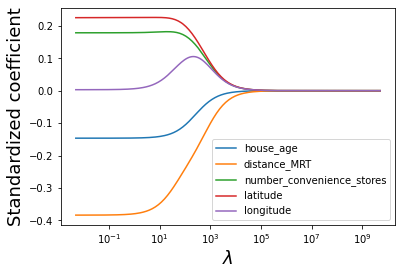
\includegraphics[keepaspectratio]{Lec1_SimpleLinearRegression_files/figure-pdf/cell-8-output-1.png}}

Note that the above plot can be made directly using the seaborn function
\texttt{regplot()}. The function \texttt{regplot()} fits a simple linear
regression model with \texttt{y} as the response, and \texttt{x} as the
predictor, and then plots the model over a scatteplot of the data.

\begin{Shaded}
\begin{Highlighting}[]
\NormalTok{ax }\OperatorTok{=}\NormalTok{ sns.regplot(x }\OperatorTok{=} \StringTok{\textquotesingle{}engineSize\textquotesingle{}}\NormalTok{, y }\OperatorTok{=} \StringTok{\textquotesingle{}price\textquotesingle{}}\NormalTok{, data }\OperatorTok{=}\NormalTok{ train, color }\OperatorTok{=} \StringTok{\textquotesingle{}orange\textquotesingle{}}\NormalTok{,line\_kws}\OperatorTok{=}\NormalTok{\{}\StringTok{"color"}\NormalTok{: }\StringTok{"blue"}\NormalTok{\})}
\NormalTok{plt.xlim(}\OperatorTok{{-}}\DecValTok{1}\NormalTok{,}\DecValTok{7}\NormalTok{)}
\NormalTok{plt.xlabel(}\StringTok{\textquotesingle{}Engine size (in litres)\textquotesingle{}}\NormalTok{)}
\NormalTok{plt.ylabel(}\StringTok{\textquotesingle{}Car price\textquotesingle{}}\NormalTok{)}
\NormalTok{ax.yaxis.set\_major\_formatter(}\StringTok{\textquotesingle{}$}\SpecialCharTok{\{x:,.0f\}}\StringTok{\textquotesingle{}}\NormalTok{)}
\NormalTok{ax.legend(handles}\OperatorTok{=}\NormalTok{legend\_elements, loc}\OperatorTok{=}\StringTok{\textquotesingle{}upper left\textquotesingle{}}\NormalTok{)}\OperatorTok{;}
\CommentTok{\#Note that some of the engineSize values are 0. They are incorrect, and should ideally be imputed before developing the model.}
\end{Highlighting}
\end{Shaded}

\pandocbounded{\includegraphics[keepaspectratio]{Lec1_SimpleLinearRegression_files/figure-pdf/cell-9-output-1.png}}

The light shaded region around the blue line in the above plot is the
confidence interval.

\textbf{Predict the car price for the cars in the test dataset}.
Datasets to be used: \emph{Car\_features\_test.csv,
Car\_prices\_test.csv}

Now that the model has been trained, let us evaluate it on unseen data.
Make sure that the columns names of the predictors are the same in train
and test datasets.

\begin{Shaded}
\begin{Highlighting}[]
\CommentTok{\# Read the test data}
\NormalTok{testf }\OperatorTok{=}\NormalTok{ pd.read\_csv(}\StringTok{\textquotesingle{}./Datasets/Car\_features\_test.csv\textquotesingle{}}\NormalTok{) }\CommentTok{\# Predictors}
\NormalTok{testp }\OperatorTok{=}\NormalTok{ pd.read\_csv(}\StringTok{\textquotesingle{}./Datasets/Car\_prices\_test.csv\textquotesingle{}}\NormalTok{) }\CommentTok{\# Response}
\NormalTok{test }\OperatorTok{=}\NormalTok{ pd.merge(testf, testp)}
\end{Highlighting}
\end{Shaded}

\begin{Shaded}
\begin{Highlighting}[]
\CommentTok{\#Using the predict() function associated with the \textquotesingle{}model\textquotesingle{} object to make predictions of car price on test (unknown) data}
\NormalTok{pred\_price }\OperatorTok{=}\NormalTok{ model.predict(testf)}\CommentTok{\#Note that the predict() function finds the predictor \textquotesingle{}engineSize\textquotesingle{} in the testf dataframe, and plugs its values in the regression equation for prediction.}
\end{Highlighting}
\end{Shaded}

\textbf{Make a visualization that compares the predicted car prices with
the actual car prices}

\begin{Shaded}
\begin{Highlighting}[]
\NormalTok{sns.scatterplot(x }\OperatorTok{=}\NormalTok{ testp.price, y }\OperatorTok{=}\NormalTok{ pred\_price, color }\OperatorTok{=} \StringTok{\textquotesingle{}orange\textquotesingle{}}\NormalTok{)}
\CommentTok{\#In case of a perfect prediction, all the points must lie on the line x = y.}
\NormalTok{ax }\OperatorTok{=}\NormalTok{ sns.lineplot(x }\OperatorTok{=}\NormalTok{ [}\DecValTok{0}\NormalTok{,testp.price.}\BuiltInTok{max}\NormalTok{()], y }\OperatorTok{=}\NormalTok{ [}\DecValTok{0}\NormalTok{,testp.price.}\BuiltInTok{max}\NormalTok{()],color}\OperatorTok{=}\StringTok{\textquotesingle{}blue\textquotesingle{}}\NormalTok{) }\CommentTok{\#Plotting the line x = y.}
\NormalTok{plt.xlabel(}\StringTok{\textquotesingle{}Actual price\textquotesingle{}}\NormalTok{)}
\NormalTok{plt.ylabel(}\StringTok{\textquotesingle{}Predicted price\textquotesingle{}}\NormalTok{)}
\NormalTok{ax.yaxis.set\_major\_formatter(}\StringTok{\textquotesingle{}$}\SpecialCharTok{\{x:,.0f\}}\StringTok{\textquotesingle{}}\NormalTok{)}
\NormalTok{ax.xaxis.set\_major\_formatter(}\StringTok{\textquotesingle{}$}\SpecialCharTok{\{x:,.0f\}}\StringTok{\textquotesingle{}}\NormalTok{)}
\NormalTok{plt.xticks(rotation}\OperatorTok{=}\DecValTok{20}\NormalTok{)}\OperatorTok{;}
\end{Highlighting}
\end{Shaded}

\pandocbounded{\includegraphics[keepaspectratio]{Lec1_SimpleLinearRegression_files/figure-pdf/cell-12-output-1.png}}

The prediction doesn't look too good. This is because we are just using
one predictor - engine size. We can probably improve the model by adding
more predictors when we learn multiple linear regression.

\textbf{What is the RMSE of the predicted car price on unseen data?}

\begin{Shaded}
\begin{Highlighting}[]
\NormalTok{np.sqrt(((testp.price }\OperatorTok{{-}}\NormalTok{ pred\_price)}\OperatorTok{**}\DecValTok{2}\NormalTok{).mean())}
\end{Highlighting}
\end{Shaded}

\begin{verbatim}
12995.106451548696
\end{verbatim}

The root mean squared error in predicting car price is around \$13k.

\textbf{What is the residual standard error based on the training data?}

\begin{Shaded}
\begin{Highlighting}[]
\NormalTok{np.sqrt(model.mse\_resid)}
\end{Highlighting}
\end{Shaded}

\begin{verbatim}
12810.109175214138
\end{verbatim}

The residual standard error on the training data is close to the RMSE on
the test data. This shows that the performance of the model on unknown
data is comparable to its performance on known data. This implies that
the model is not overfitting, which is good! In case we overfit a model
on the training data, its performance on unknown data is likely to be
worse than that on the training data.

\textbf{Find the confidence and prediction intervals of the predicted
car price}

\begin{Shaded}
\begin{Highlighting}[]
\CommentTok{\#Using the get\_prediction() function associated with the \textquotesingle{}model\textquotesingle{} object to get the intervals}
\NormalTok{intervals }\OperatorTok{=}\NormalTok{ model.get\_prediction(testf)}
\end{Highlighting}
\end{Shaded}

\begin{Shaded}
\begin{Highlighting}[]
\CommentTok{\#The function requires specifying alpha (probability of Type 1 error) instead of the confidence level to get the intervals}
\NormalTok{intervals.summary\_frame(alpha}\OperatorTok{=}\FloatTok{0.05}\NormalTok{)}
\end{Highlighting}
\end{Shaded}

\begin{longtable}[]{@{}lllllll@{}}
\toprule\noalign{}
& mean & mean\_se & mean\_ci\_lower & mean\_ci\_upper & obs\_ci\_lower &
obs\_ci\_upper \\
\midrule\noalign{}
\endhead
\bottomrule\noalign{}
\endlastfoot
0 & 34842.807319 & 271.666459 & 34310.220826 & 35375.393812 &
9723.677232 & 59961.937406 \\
1 & 34842.807319 & 271.666459 & 34310.220826 & 35375.393812 &
9723.677232 & 59961.937406 \\
2 & 34842.807319 & 271.666459 & 34310.220826 & 35375.393812 &
9723.677232 & 59961.937406 \\
3 & 8866.245277 & 316.580850 & 8245.606701 & 9486.883853 & -16254.905974
& 33987.396528 \\
4 & 47831.088340 & 468.949360 & 46911.740050 & 48750.436631 &
22700.782946 & 72961.393735 \\
... & ... & ... & ... & ... & ... & ... \\
2667 & 47831.088340 & 468.949360 & 46911.740050 & 48750.436631 &
22700.782946 & 72961.393735 \\
2668 & 34842.807319 & 271.666459 & 34310.220826 & 35375.393812 &
9723.677232 & 59961.937406 \\
2669 & 8866.245277 & 316.580850 & 8245.606701 & 9486.883853 &
-16254.905974 & 33987.396528 \\
2670 & 21854.526298 & 184.135754 & 21493.538727 & 22215.513869 &
-3261.551421 & 46970.604017 \\
2671 & 21854.526298 & 184.135754 & 21493.538727 & 22215.513869 &
-3261.551421 & 46970.604017 \\
\end{longtable}

\textbf{Show the regression line predicting car price based on engine
size for test data. Also show the confidence and prediction intervals
for the car price.}

\begin{Shaded}
\begin{Highlighting}[]
\NormalTok{interval\_table }\OperatorTok{=}\NormalTok{ intervals.summary\_frame(alpha}\OperatorTok{=}\FloatTok{0.05}\NormalTok{)}
\end{Highlighting}
\end{Shaded}

\begin{Shaded}
\begin{Highlighting}[]
\NormalTok{ax }\OperatorTok{=}\NormalTok{ sns.scatterplot(x }\OperatorTok{=}\NormalTok{ testf.engineSize, y }\OperatorTok{=}\NormalTok{ pred\_price,color }\OperatorTok{=} \StringTok{\textquotesingle{}orange\textquotesingle{}}\NormalTok{, s }\OperatorTok{=} \DecValTok{10}\NormalTok{)}
\NormalTok{sns.lineplot(x }\OperatorTok{=}\NormalTok{ testf.engineSize, y }\OperatorTok{=}\NormalTok{ pred\_price, color }\OperatorTok{=} \StringTok{\textquotesingle{}red\textquotesingle{}}\NormalTok{)}
\NormalTok{sns.lineplot(x }\OperatorTok{=}\NormalTok{ testf.engineSize, y }\OperatorTok{=}\NormalTok{ interval\_table.mean\_ci\_lower, color }\OperatorTok{=} \StringTok{\textquotesingle{}blue\textquotesingle{}}\NormalTok{)}
\NormalTok{sns.lineplot(x }\OperatorTok{=}\NormalTok{ testf.engineSize, y }\OperatorTok{=}\NormalTok{ interval\_table.mean\_ci\_upper, color }\OperatorTok{=} \StringTok{\textquotesingle{}blue\textquotesingle{}}\NormalTok{)}
\NormalTok{sns.lineplot(x }\OperatorTok{=}\NormalTok{ testf.engineSize, y }\OperatorTok{=}\NormalTok{ interval\_table.obs\_ci\_lower, color }\OperatorTok{=} \StringTok{\textquotesingle{}green\textquotesingle{}}\NormalTok{)}
\NormalTok{sns.lineplot(x }\OperatorTok{=}\NormalTok{ testf.engineSize, y }\OperatorTok{=}\NormalTok{ interval\_table.obs\_ci\_upper, color }\OperatorTok{=} \StringTok{\textquotesingle{}green\textquotesingle{}}\NormalTok{)}

\NormalTok{legend\_elements }\OperatorTok{=}\NormalTok{ [Line2D([}\DecValTok{0}\NormalTok{], [}\DecValTok{0}\NormalTok{], color}\OperatorTok{=}\StringTok{\textquotesingle{}red\textquotesingle{}}\NormalTok{, label}\OperatorTok{=}\StringTok{\textquotesingle{}Mean prediction\textquotesingle{}}\NormalTok{),}
\NormalTok{                   Line2D([}\DecValTok{0}\NormalTok{], [}\DecValTok{0}\NormalTok{], color}\OperatorTok{=}\StringTok{\textquotesingle{}blue\textquotesingle{}}\NormalTok{, label}\OperatorTok{=}\StringTok{\textquotesingle{}Confidence interval\textquotesingle{}}\NormalTok{),}
\NormalTok{                  Line2D([}\DecValTok{0}\NormalTok{], [}\DecValTok{0}\NormalTok{], color}\OperatorTok{=}\StringTok{\textquotesingle{}green\textquotesingle{}}\NormalTok{, label}\OperatorTok{=}\StringTok{\textquotesingle{}Prediction interval\textquotesingle{}}\NormalTok{)]}
\NormalTok{ax.legend(handles}\OperatorTok{=}\NormalTok{legend\_elements, loc}\OperatorTok{=}\StringTok{\textquotesingle{}upper left\textquotesingle{}}\NormalTok{)}
\NormalTok{plt.xlabel(}\StringTok{\textquotesingle{}Engine size (in litres)\textquotesingle{}}\NormalTok{)}
\NormalTok{plt.ylabel(}\StringTok{\textquotesingle{}Car price\textquotesingle{}}\NormalTok{)}
\NormalTok{ax.yaxis.set\_major\_formatter(}\StringTok{\textquotesingle{}$}\SpecialCharTok{\{x:,.0f\}}\StringTok{\textquotesingle{}}\NormalTok{)}\OperatorTok{;}
\end{Highlighting}
\end{Shaded}

\pandocbounded{\includegraphics[keepaspectratio]{Lec1_SimpleLinearRegression_files/figure-pdf/cell-18-output-1.png}}

\subsection{\texorpdfstring{Training with
\href{https://scikit-learn.org/stable/}{\texttt{sklearn}}}{Training with sklearn}}\label{training-with-sklearn}

\begin{Shaded}
\begin{Highlighting}[]
\CommentTok{\# Create the model as an object}

\NormalTok{model }\OperatorTok{=}\NormalTok{ LinearRegression() }\CommentTok{\# No inputs, this will change for other models}

\CommentTok{\# Train the model {-} separate the predictor(s) and the response for this!}
\NormalTok{X\_train }\OperatorTok{=}\NormalTok{ train[[}\StringTok{\textquotesingle{}engineSize\textquotesingle{}}\NormalTok{]]}
\NormalTok{y\_train }\OperatorTok{=}\NormalTok{ train[[}\StringTok{\textquotesingle{}price\textquotesingle{}}\NormalTok{]]}

\CommentTok{\# Note that both are dfs, NOT series {-} necessary to avoid errors}

\NormalTok{model.fit(X\_train, y\_train)}

\CommentTok{\# Check the slight syntax differences}
    \CommentTok{\# predictors and response separate}
    \CommentTok{\# We need to manually slice the predictor column(s) we want to include}
    \CommentTok{\# No need to assign to an output}
    
\CommentTok{\# Return the parameters}
\BuiltInTok{print}\NormalTok{(}\StringTok{"Coefficient of engine size = "}\NormalTok{, model.coef\_) }\CommentTok{\# slope}
\BuiltInTok{print}\NormalTok{(}\StringTok{"Intercept = "}\NormalTok{, model.intercept\_) }\CommentTok{\# intercept}

\CommentTok{\# No .summary() here! {-} impossible to do much inference; this is a shortcoming of sklearn}
\end{Highlighting}
\end{Shaded}

\begin{verbatim}
Coefficient of engine size =  [[12988.28102112]]
Intercept =  [-4122.03574424]
\end{verbatim}

\begin{Shaded}
\begin{Highlighting}[]
\CommentTok{\# Prediction}

\CommentTok{\# Again, separate the predictor(s) and the response of interest}
\NormalTok{X\_test }\OperatorTok{=}\NormalTok{ test[[}\StringTok{\textquotesingle{}engineSize\textquotesingle{}}\NormalTok{]]}
\NormalTok{y\_test }\OperatorTok{=}\NormalTok{ test[[}\StringTok{\textquotesingle{}price\textquotesingle{}}\NormalTok{]].to\_numpy() }\CommentTok{\# Easier to handle with calculations as np array}

\NormalTok{y\_pred }\OperatorTok{=}\NormalTok{ model.predict(X\_test)}

\CommentTok{\# Evaluate}
\NormalTok{model\_rmse }\OperatorTok{=}\NormalTok{ np.sqrt(np.mean((y\_pred }\OperatorTok{{-}}\NormalTok{ y\_test)}\OperatorTok{**}\DecValTok{2}\NormalTok{)) }\CommentTok{\# RMSE}
\NormalTok{model\_mae }\OperatorTok{=}\NormalTok{ np.mean(np.}\BuiltInTok{abs}\NormalTok{(y\_pred }\OperatorTok{{-}}\NormalTok{ y\_test)) }\CommentTok{\# MAE}

\BuiltInTok{print}\NormalTok{(}\StringTok{\textquotesingle{}Test RMSE: \textquotesingle{}}\NormalTok{, model\_rmse)}
\end{Highlighting}
\end{Shaded}

\begin{verbatim}
Test RMSE:  12995.106451548696
\end{verbatim}

\begin{Shaded}
\begin{Highlighting}[]
\CommentTok{\# Easier way to calculate metrics with sklearn tools}

\CommentTok{\# Note that we have imported the functions \textquotesingle{}mean\_squared\_error\textquotesingle{} and \textquotesingle{}mean\_absolute\_error\textquotesingle{}}
\CommentTok{\# from the sklearn.metrics module (check top of the code)}

\NormalTok{model\_rmse }\OperatorTok{=}\NormalTok{ np.sqrt(mean\_squared\_error(y\_test,y\_pred))}
\NormalTok{model\_mae }\OperatorTok{=}\NormalTok{ mean\_absolute\_error(y\_test,y\_pred)}
\BuiltInTok{print}\NormalTok{(}\StringTok{\textquotesingle{}Test RMSE: \textquotesingle{}}\NormalTok{, model\_rmse)}
\BuiltInTok{print}\NormalTok{(}\StringTok{\textquotesingle{}Test MAE: \textquotesingle{}}\NormalTok{, model\_mae)}
\end{Highlighting}
\end{Shaded}

\begin{verbatim}
Test RMSE:  12995.106451548696
Test MAE:  9411.325912951994
\end{verbatim}

\begin{Shaded}
\begin{Highlighting}[]
\NormalTok{y\_pred\_train }\OperatorTok{=}\NormalTok{ model.predict(X\_train)}
\BuiltInTok{print}\NormalTok{(}\StringTok{\textquotesingle{}Train R{-}squared:\textquotesingle{}}\NormalTok{, r2\_score(y\_train, y\_pred\_train))}
\BuiltInTok{print}\NormalTok{(}\StringTok{\textquotesingle{}Test R{-}squared:\textquotesingle{}}\NormalTok{, r2\_score(y\_test, y\_pred))}
\end{Highlighting}
\end{Shaded}

\begin{verbatim}
Train R-squared: 0.39049842625794573
Test R-squared: 0.3869900378620146
\end{verbatim}

\textbf{Note:} Why did we repeat the same task in two different
libraries?

\begin{itemize}
\tightlist
\item
  \texttt{statsmodels} and \texttt{sklearn} have different advantages -
  we will use both for our purposes

  \begin{itemize}
  \tightlist
  \item
    \texttt{statsmodels} returns a lot of statistical output, which is
    very helpful for inference (coming up next) but it has a limited
    variety of models.
  \item
    With \texttt{statsmodels}, you may have columns in your DataFrame in
    addition to predictors and response, while with \texttt{sklearn} you
    need to make separate objects consisting of only the predictors and
    the response.
  \item
    \texttt{sklearn} includes many models (\texttt{Lasso} and
    \texttt{Ridge} this quarter, many others next quarter) and helpful
    tools/functions (like metrics) that statsmodels does not but it does
    not have any inference tools.
  \end{itemize}
\end{itemize}

\subsection{\texorpdfstring{Training with
\texttt{statsmodels.api}}{Training with statsmodels.api}}\label{training-with-statsmodels.api}

Earlier we had used the \texttt{statsmodels.formula.api} module, where
we had to put the regression model as a formula. We can also use the
\texttt{statsmodels.api} module to develop a regression model. The
syntax of training a model with the \texttt{OLS()} function in this
module is similar to that of \texttt{sklearn}'s
\texttt{LinearRegression()} function. However, the order in which the
predictors and response are specified is different. The formula-style
syntax of the \texttt{statsmodels.formula.api} module is generally
preferred. However, depending on the situation, the \texttt{OLS()}
syntax of \texttt{statsmodels.api} may be preferred.

Note that you will manually need to add the predictor \emph{(a column of
ones)} corresponding to the intercept to train the model with this
method.

\begin{Shaded}
\begin{Highlighting}[]
\CommentTok{\# Create the model as an object}

\CommentTok{\# Train the model {-} separate the predictor(s) and the response for this!}
\NormalTok{X\_train }\OperatorTok{=}\NormalTok{ train[[}\StringTok{\textquotesingle{}engineSize\textquotesingle{}}\NormalTok{]]}
\NormalTok{y\_train }\OperatorTok{=}\NormalTok{ train[[}\StringTok{\textquotesingle{}price\textquotesingle{}}\NormalTok{]]}

\NormalTok{X\_train\_with\_intercept }\OperatorTok{=}\NormalTok{ np.concatenate((np.ones(X\_train.shape[}\DecValTok{0}\NormalTok{]).reshape(}\OperatorTok{{-}}\DecValTok{1}\NormalTok{,}\DecValTok{1}\NormalTok{), X\_train), axis }\OperatorTok{=} \DecValTok{1}\NormalTok{)}

\NormalTok{model }\OperatorTok{=}\NormalTok{ sm.OLS(y\_train, X\_train\_with\_intercept).fit()}
    
\CommentTok{\# Return the parameters}
\BuiltInTok{print}\NormalTok{(model.params) }
\end{Highlighting}
\end{Shaded}

\begin{verbatim}
const    -4122.035744
x1       12988.281021
dtype: float64
\end{verbatim}

The model summary and all other attributes and methods of the
\texttt{model} object are the same as that with the object created using
the \texttt{statsmodels.formula.api} module.

\begin{Shaded}
\begin{Highlighting}[]
\NormalTok{model.summary()}
\end{Highlighting}
\end{Shaded}

\begin{center}
\begin{tabular}{lclc}
\toprule
\textbf{Dep. Variable:}    &      price       & \textbf{  R-squared:         } &     0.390   \\
\textbf{Model:}            &       OLS        & \textbf{  Adj. R-squared:    } &     0.390   \\
\textbf{Method:}           &  Least Squares   & \textbf{  F-statistic:       } &     3177.   \\
\textbf{Date:}             & Mon, 08 Jan 2024 & \textbf{  Prob (F-statistic):} &     0.00    \\
\textbf{Time:}             &     11:17:55     & \textbf{  Log-Likelihood:    } &   -53949.   \\
\textbf{No. Observations:} &        4960      & \textbf{  AIC:               } & 1.079e+05   \\
\textbf{Df Residuals:}     &        4958      & \textbf{  BIC:               } & 1.079e+05   \\
\textbf{Df Model:}         &           1      & \textbf{                     } &             \\
\textbf{Covariance Type:}  &    nonrobust     & \textbf{                     } &             \\
\bottomrule
\end{tabular}
\begin{tabular}{lcccccc}
               & \textbf{coef} & \textbf{std err} & \textbf{t} & \textbf{P$> |$t$|$} & \textbf{[0.025} & \textbf{0.975]}  \\
\midrule
\textbf{const} &   -4122.0357  &      522.260     &    -7.893  &         0.000        &    -5145.896    &    -3098.176     \\
\textbf{x1}    &    1.299e+04  &      230.450     &    56.361  &         0.000        &     1.25e+04    &     1.34e+04     \\
\bottomrule
\end{tabular}
\begin{tabular}{lclc}
\textbf{Omnibus:}       & 1271.986 & \textbf{  Durbin-Watson:     } &    0.517  \\
\textbf{Prob(Omnibus):} &   0.000  & \textbf{  Jarque-Bera (JB):  } & 6490.719  \\
\textbf{Skew:}          &   1.137  & \textbf{  Prob(JB):          } &     0.00  \\
\textbf{Kurtosis:}      &   8.122  & \textbf{  Cond. No.          } &     7.64  \\
\bottomrule
\end{tabular}
%\caption{OLS Regression Results}
\end{center}

Notes: \newline
 [1] Standard Errors assume that the covariance matrix of the errors is correctly specified.

\bookmarksetup{startatroot}

\chapter{Multiple Linear Regression}\label{multiple-linear-regression}

\emph{Read section 3.2 of the book before using these notes.}

\emph{Note that in this course, lecture notes are not sufficient, you
must read the book for better understanding. Lecture notes are just
implementing the concepts of the book on a dataset, but not explaining
the concepts elaborately.}

\section{Multiple Linear Regression}\label{multiple-linear-regression-1}

\begin{Shaded}
\begin{Highlighting}[]
\CommentTok{\# importing libraries }
\ImportTok{import}\NormalTok{ pandas }\ImportTok{as}\NormalTok{ pd}
\ImportTok{import}\NormalTok{ numpy }\ImportTok{as}\NormalTok{ np}
\ImportTok{import}\NormalTok{ statsmodels.formula.api }\ImportTok{as}\NormalTok{ smf}
\ImportTok{import}\NormalTok{ seaborn }\ImportTok{as}\NormalTok{ sns}
\ImportTok{import}\NormalTok{ matplotlib.pyplot }\ImportTok{as}\NormalTok{ plt}
\ImportTok{from}\NormalTok{ sklearn.linear\_model }\ImportTok{import}\NormalTok{ LinearRegression}
\end{Highlighting}
\end{Shaded}

\textbf{Develop a multiple linear regression model that predicts car
price based on engine size, year, mileage, and mpg.} Datasets to be
used: \emph{Car\_features\_train.csv, Car\_prices\_train.csv}

\begin{Shaded}
\begin{Highlighting}[]
\CommentTok{\# Reading datasets}
\NormalTok{trainf }\OperatorTok{=}\NormalTok{ pd.read\_csv(}\StringTok{\textquotesingle{}./Datasets/Car\_features\_train.csv\textquotesingle{}}\NormalTok{)}
\NormalTok{trainp }\OperatorTok{=}\NormalTok{ pd.read\_csv(}\StringTok{\textquotesingle{}./Datasets/Car\_prices\_train.csv\textquotesingle{}}\NormalTok{)}
\NormalTok{train }\OperatorTok{=}\NormalTok{ pd.merge(trainf,trainp)}
\NormalTok{train.head()}
\end{Highlighting}
\end{Shaded}

\begin{longtable}[]{@{}llllllllllll@{}}
\toprule\noalign{}
& carID & brand & model & year & transmission & mileage & fuelType & tax
& mpg & engineSize & price \\
\midrule\noalign{}
\endhead
\bottomrule\noalign{}
\endlastfoot
0 & 18473 & bmw & 6 Series & 2020 & Semi-Auto & 11 & Diesel & 145 &
53.3282 & 3.0 & 37980 \\
1 & 15064 & bmw & 6 Series & 2019 & Semi-Auto & 10813 & Diesel & 145 &
53.0430 & 3.0 & 33980 \\
2 & 18268 & bmw & 6 Series & 2020 & Semi-Auto & 6 & Diesel & 145 &
53.4379 & 3.0 & 36850 \\
3 & 18480 & bmw & 6 Series & 2017 & Semi-Auto & 18895 & Diesel & 145 &
51.5140 & 3.0 & 25998 \\
4 & 18492 & bmw & 6 Series & 2015 & Automatic & 62953 & Diesel & 160 &
51.4903 & 3.0 & 18990 \\
\end{longtable}

\subsection{Training the model}\label{training-the-model}

\begin{Shaded}
\begin{Highlighting}[]
\CommentTok{\#Using the ols function to create an ols object. \textquotesingle{}ols\textquotesingle{} stands for \textquotesingle{}Ordinary least squares\textquotesingle{}}
\NormalTok{ols\_object }\OperatorTok{=}\NormalTok{ smf.ols(formula }\OperatorTok{=} \StringTok{\textquotesingle{}price\textasciitilde{}year+mileage+mpg+engineSize\textquotesingle{}}\NormalTok{, data }\OperatorTok{=}\NormalTok{ train)}
\NormalTok{model }\OperatorTok{=}\NormalTok{ ols\_object.fit()}
\NormalTok{model.summary()}
\end{Highlighting}
\end{Shaded}

\begin{center}
\begin{tabular}{lclc}
\toprule
\textbf{Dep. Variable:}    &      price       & \textbf{  R-squared:         } &     0.660   \\
\textbf{Model:}            &       OLS        & \textbf{  Adj. R-squared:    } &     0.660   \\
\textbf{Method:}           &  Least Squares   & \textbf{  F-statistic:       } &     2410.   \\
\textbf{Date:}             & Mon, 29 Jan 2024 & \textbf{  Prob (F-statistic):} &     0.00    \\
\textbf{Time:}             &     03:10:20     & \textbf{  Log-Likelihood:    } &   -52497.   \\
\textbf{No. Observations:} &        4960      & \textbf{  AIC:               } & 1.050e+05   \\
\textbf{Df Residuals:}     &        4955      & \textbf{  BIC:               } & 1.050e+05   \\
\textbf{Df Model:}         &           4      & \textbf{                     } &             \\
\textbf{Covariance Type:}  &    nonrobust     & \textbf{                     } &             \\
\bottomrule
\end{tabular}
\begin{tabular}{lcccccc}
                    & \textbf{coef} & \textbf{std err} & \textbf{t} & \textbf{P$> |$t$|$} & \textbf{[0.025} & \textbf{0.975]}  \\
\midrule
\textbf{Intercept}  &   -3.661e+06  &     1.49e+05     &   -24.593  &         0.000        &    -3.95e+06    &    -3.37e+06     \\
\textbf{year}       &    1817.7366  &       73.751     &    24.647  &         0.000        &     1673.151    &     1962.322     \\
\textbf{mileage}    &      -0.1474  &        0.009     &   -16.817  &         0.000        &       -0.165    &       -0.130     \\
\textbf{mpg}        &     -79.3126  &        9.338     &    -8.493  &         0.000        &      -97.620    &      -61.006     \\
\textbf{engineSize} &    1.218e+04  &      189.969     &    64.107  &         0.000        &     1.18e+04    &     1.26e+04     \\
\bottomrule
\end{tabular}
\begin{tabular}{lclc}
\textbf{Omnibus:}       & 2450.973 & \textbf{  Durbin-Watson:     } &     0.541  \\
\textbf{Prob(Omnibus):} &   0.000  & \textbf{  Jarque-Bera (JB):  } & 31060.548  \\
\textbf{Skew:}          &   2.045  & \textbf{  Prob(JB):          } &      0.00  \\
\textbf{Kurtosis:}      &  14.557  & \textbf{  Cond. No.          } &  3.83e+07  \\
\bottomrule
\end{tabular}
%\caption{OLS Regression Results}
\end{center}

Notes: \newline
 [1] Standard Errors assume that the covariance matrix of the errors is correctly specified. \newline
 [2] The condition number is large, 3.83e+07. This might indicate that there are \newline
 strong multicollinearity or other numerical problems.

The model equation is: estimated car \texttt{price} = -3.661e6 + 1818 *
\texttt{year} -0.15 * \texttt{mileage} - 79.31 * \texttt{mpg} + 12180 *
\texttt{engineSize}

The procedure to fit the model using \texttt{sklearn} will be similar to
that in simple linear regression.

\begin{Shaded}
\begin{Highlighting}[]
\NormalTok{model }\OperatorTok{=}\NormalTok{ LinearRegression()}

\NormalTok{X\_train }\OperatorTok{=}\NormalTok{ train[[}\StringTok{\textquotesingle{}year\textquotesingle{}}\NormalTok{,}\StringTok{\textquotesingle{}engineSize\textquotesingle{}}\NormalTok{,}\StringTok{\textquotesingle{}mpg\textquotesingle{}}\NormalTok{,}\StringTok{\textquotesingle{}mileage\textquotesingle{}}\NormalTok{]] }\CommentTok{\# Slice out the predictors}
\NormalTok{y\_train }\OperatorTok{=}\NormalTok{ train[[}\StringTok{\textquotesingle{}price\textquotesingle{}}\NormalTok{]]}

\NormalTok{model.fit(X\_train,y\_train)}
\end{Highlighting}
\end{Shaded}

\subsection{Hypothesis test for a relationship between the response and
a subset of
predictors}\label{hypothesis-test-for-a-relationship-between-the-response-and-a-subset-of-predictors}

Let us test the hypothesis if there is relationship between car price
and the set of predictors: \texttt{mpg} and \texttt{year}.

\begin{Shaded}
\begin{Highlighting}[]
\NormalTok{hypothesis }\OperatorTok{=} \StringTok{\textquotesingle{}(mpg = 0, year = 0)\textquotesingle{}}     
    
\NormalTok{model.f\_test(hypothesis) }\CommentTok{\# the F test of these two predictors is stat. sig.}
\end{Highlighting}
\end{Shaded}

\begin{verbatim}
<class 'statsmodels.stats.contrast.ContrastResults'>
<F test: F=325.9206432972666, p=1.0499509223096256e-133, df_denom=4.96e+03, df_num=2>
\end{verbatim}

As the \(p\)-value is low, we reject the null hypothesis, i.e., at least
one of the predictors among \texttt{mpg} and \texttt{year} has a
statistically significant relationship with car price.

\textbf{Predict the car price for the cars in the test dataset}.
Datasets to be used: \emph{Car\_features\_test.csv,
Car\_prices\_test.csv}

\begin{Shaded}
\begin{Highlighting}[]
\NormalTok{testf }\OperatorTok{=}\NormalTok{ pd.read\_csv(}\StringTok{\textquotesingle{}./Datasets/Car\_features\_test.csv\textquotesingle{}}\NormalTok{)}
\NormalTok{testp }\OperatorTok{=}\NormalTok{ pd.read\_csv(}\StringTok{\textquotesingle{}./Datasets/Car\_prices\_test.csv\textquotesingle{}}\NormalTok{)}
\end{Highlighting}
\end{Shaded}

\subsection{Prediction}\label{prediction}

\begin{Shaded}
\begin{Highlighting}[]
\NormalTok{pred\_price }\OperatorTok{=}\NormalTok{ model.predict(testf)}
\end{Highlighting}
\end{Shaded}

\textbf{Make a visualization that compares the predicted car prices with
the actual car prices}

\begin{Shaded}
\begin{Highlighting}[]
\NormalTok{sns.}\BuiltInTok{set}\NormalTok{(font\_scale}\OperatorTok{=}\FloatTok{1.25}\NormalTok{)}
\NormalTok{sns.scatterplot(x }\OperatorTok{=}\NormalTok{ testp.price, y }\OperatorTok{=}\NormalTok{ pred\_price, color }\OperatorTok{=} \StringTok{\textquotesingle{}orange\textquotesingle{}}\NormalTok{)}
\CommentTok{\#In case of a perfect prediction, all the points must lie on the line x = y.}
\NormalTok{ax }\OperatorTok{=}\NormalTok{ sns.lineplot(x }\OperatorTok{=}\NormalTok{ [}\DecValTok{0}\NormalTok{,testp.price.}\BuiltInTok{max}\NormalTok{()], y }\OperatorTok{=}\NormalTok{ [}\DecValTok{0}\NormalTok{,testp.price.}\BuiltInTok{max}\NormalTok{()],color}\OperatorTok{=}\StringTok{\textquotesingle{}blue\textquotesingle{}}\NormalTok{) }\CommentTok{\#Plotting the line x = y.}
\NormalTok{plt.xlabel(}\StringTok{\textquotesingle{}Actual price\textquotesingle{}}\NormalTok{)}
\NormalTok{plt.ylabel(}\StringTok{\textquotesingle{}Predicted price\textquotesingle{}}\NormalTok{)}
\NormalTok{plt.ylim([}\OperatorTok{{-}}\DecValTok{10000}\NormalTok{, }\DecValTok{160000}\NormalTok{])}
\NormalTok{ax.yaxis.set\_major\_formatter(}\StringTok{\textquotesingle{}$}\SpecialCharTok{\{x:,.0f\}}\StringTok{\textquotesingle{}}\NormalTok{)}
\NormalTok{ax.xaxis.set\_major\_formatter(}\StringTok{\textquotesingle{}$}\SpecialCharTok{\{x:,.0f\}}\StringTok{\textquotesingle{}}\NormalTok{)}
\NormalTok{plt.xticks(rotation}\OperatorTok{=}\DecValTok{20}\NormalTok{)}\OperatorTok{;}
\end{Highlighting}
\end{Shaded}

\pandocbounded{\includegraphics[keepaspectratio]{Lec2_MultipleLinearRegression_files/figure-pdf/cell-9-output-1.png}}

The prediction looks better as compared to the one with simple linear
regression. This is because we have four predictors to help explain the
variation in car price, instead of just one in the case of simple linear
regression. Also, all the predictors have a significant relationship
with price as evident from their p-values. Thus, all four of them are
contributing in explaining the variation. Note the higher values of
\(R^2\) as compared to the one in the case of simple linear regression.

\textbf{What is the RMSE of the predicted car price?}

\begin{Shaded}
\begin{Highlighting}[]
\NormalTok{np.sqrt(((testp.price }\OperatorTok{{-}}\NormalTok{ pred\_price)}\OperatorTok{**}\DecValTok{2}\NormalTok{).mean())}
\end{Highlighting}
\end{Shaded}

\begin{verbatim}
9956.82497993548
\end{verbatim}

\textbf{What is the residual standard error based on the training data?}

\begin{Shaded}
\begin{Highlighting}[]
\NormalTok{np.sqrt(model.mse\_resid)}
\end{Highlighting}
\end{Shaded}

\begin{verbatim}
9563.74782917604
\end{verbatim}

\begin{Shaded}
\begin{Highlighting}[]
\NormalTok{trainp.describe()}
\end{Highlighting}
\end{Shaded}

\begin{longtable}[]{@{}lll@{}}
\toprule\noalign{}
& carID & price \\
\midrule\noalign{}
\endhead
\bottomrule\noalign{}
\endlastfoot
count & 4960.000000 & 4960.000000 \\
mean & 15832.446169 & 23469.943750 \\
std & 2206.717006 & 16406.714563 \\
min & 12002.000000 & 450.000000 \\
25\% & 13929.250000 & 12000.000000 \\
50\% & 15840.000000 & 18999.000000 \\
75\% & 17765.750000 & 30335.750000 \\
max & 19629.000000 & 145000.000000 \\
\end{longtable}

\begin{Shaded}
\begin{Highlighting}[]
\NormalTok{sns.scatterplot(x }\OperatorTok{=}\NormalTok{ model.fittedvalues, y}\OperatorTok{=}\NormalTok{model.resid,color }\OperatorTok{=} \StringTok{\textquotesingle{}orange\textquotesingle{}}\NormalTok{)}
\NormalTok{ax }\OperatorTok{=}\NormalTok{ sns.lineplot(x }\OperatorTok{=}\NormalTok{ [pred\_price.}\BuiltInTok{min}\NormalTok{(),pred\_price.}\BuiltInTok{max}\NormalTok{()],y }\OperatorTok{=}\NormalTok{ [}\DecValTok{0}\NormalTok{,}\DecValTok{0}\NormalTok{],color }\OperatorTok{=} \StringTok{\textquotesingle{}blue\textquotesingle{}}\NormalTok{)}
\NormalTok{plt.xlabel(}\StringTok{\textquotesingle{}Predicted price\textquotesingle{}}\NormalTok{)}
\NormalTok{plt.ylabel(}\StringTok{\textquotesingle{}Residual\textquotesingle{}}\NormalTok{)}
\NormalTok{ax.yaxis.set\_major\_formatter(}\StringTok{\textquotesingle{}$}\SpecialCharTok{\{x:,.0f\}}\StringTok{\textquotesingle{}}\NormalTok{)}
\NormalTok{ax.xaxis.set\_major\_formatter(}\StringTok{\textquotesingle{}$}\SpecialCharTok{\{x:,.0f\}}\StringTok{\textquotesingle{}}\NormalTok{)}
\NormalTok{plt.xticks(rotation}\OperatorTok{=}\DecValTok{20}\NormalTok{)}\OperatorTok{;}
\end{Highlighting}
\end{Shaded}

\pandocbounded{\includegraphics[keepaspectratio]{Lec2_MultipleLinearRegression_files/figure-pdf/cell-13-output-1.png}}

\subsection{\texorpdfstring{Effect of adding noisy predictors on
\(R^2\)}{Effect of adding noisy predictors on R\^{}2}}\label{effect-of-adding-noisy-predictors-on-r2}

\textbf{Will the explained variation (R-squared) in car price always
increase if we add a variable?}

\textbf{Should we keep on adding variables as long as the explained
variation (R-squared) is increasing?}

\begin{Shaded}
\begin{Highlighting}[]
\CommentTok{\#Using the ols function to create an ols object. \textquotesingle{}ols\textquotesingle{} stands for \textquotesingle{}Ordinary least squares\textquotesingle{}}
\NormalTok{np.random.seed(}\DecValTok{1}\NormalTok{)}
\NormalTok{train[}\StringTok{\textquotesingle{}rand\_col\textquotesingle{}}\NormalTok{] }\OperatorTok{=}\NormalTok{ np.random.rand(train.shape[}\DecValTok{0}\NormalTok{])}
\NormalTok{ols\_object }\OperatorTok{=}\NormalTok{ smf.ols(formula }\OperatorTok{=} \StringTok{\textquotesingle{}price\textasciitilde{}year+mileage+mpg+engineSize+rand\_col\textquotesingle{}}\NormalTok{, data }\OperatorTok{=}\NormalTok{ train)}
\NormalTok{model }\OperatorTok{=}\NormalTok{ ols\_object.fit()}
\NormalTok{model.summary()}
\end{Highlighting}
\end{Shaded}

\begin{longtable}[]{@{}llll@{}}
\caption{OLS Regression Results}\tabularnewline
\toprule\noalign{}
\endfirsthead
\endhead
\bottomrule\noalign{}
\endlastfoot
Dep. Variable: & price & R-squared: & 0.661 \\
Model: & OLS & Adj. R-squared: & 0.660 \\
Method: & Least Squares & F-statistic: & 1928. \\
Date: & Tue, 27 Dec 2022 & Prob (F-statistic): & 0.00 \\
Time: & 01:07:38 & Log-Likelihood: & -52497. \\
No. Observations: & 4960 & AIC: & 1.050e+05 \\
Df Residuals: & 4954 & BIC: & 1.050e+05 \\
Df Model: & 5 & & \\
Covariance Type: & nonrobust & & \\
\end{longtable}

\begin{longtable}[]{@{}lllllll@{}}
\toprule\noalign{}
\endhead
\bottomrule\noalign{}
\endlastfoot
& coef & std err & t & P\textgreater\textbar t\textbar{} & {[}0.025 &
0.975{]} \\
Intercept & -3.662e+06 & 1.49e+05 & -24.600 & 0.000 & -3.95e+06 &
-3.37e+06 \\
year & 1818.1672 & 73.753 & 24.652 & 0.000 & 1673.578 & 1962.756 \\
mileage & -0.1474 & 0.009 & -16.809 & 0.000 & -0.165 & -0.130 \\
mpg & -79.2837 & 9.338 & -8.490 & 0.000 & -97.591 & -60.976 \\
engineSize & 1.218e+04 & 189.972 & 64.109 & 0.000 & 1.18e+04 &
1.26e+04 \\
rand\_col & 451.1226 & 471.897 & 0.956 & 0.339 & -474.004 & 1376.249 \\
\end{longtable}

\begin{longtable}[]{@{}llll@{}}
\toprule\noalign{}
\endhead
\bottomrule\noalign{}
\endlastfoot
Omnibus: & 2451.728 & Durbin-Watson: & 0.541 \\
Prob(Omnibus): & 0.000 & Jarque-Bera (JB): & 31040.331 \\
Skew: & 2.046 & Prob(JB): & 0.00 \\
Kurtosis: & 14.552 & Cond. No. & 3.83e+07 \\
\end{longtable}

Adding a variable with random values to the model (\texttt{rand\_col})
increased the explained variation (\(R^2\)). This is because the model
has one more parameter to tune to reduce the residual squared error
\((RSS)\). However, the \(p\)-value of \texttt{rand\_col} suggests that
its coefficient is zero. Thus, using the model with \texttt{rand\_col}
may give poorer performance on unknown data, as compared to the model
without \texttt{rand\_col}. This implies that it is not a good idea to
blindly add variables in the model to increase \(R^2\).

\bookmarksetup{startatroot}

\chapter{Extending Linear Regression
(statsmodels)}\label{extending-linear-regression-statsmodels}

\emph{Read sections 3.3.1 and 3.3.2 of the book before using these
notes.}

\emph{Note that in this course, lecture notes are not sufficient, you
must read the book for better understanding. Lecture notes are just
implementing the concepts of the book on a dataset, but not explaining
the concepts elaborately.}

\section{Variable interactions}\label{variable-interactions}

\begin{Shaded}
\begin{Highlighting}[]
\ImportTok{import}\NormalTok{ pandas }\ImportTok{as}\NormalTok{ pd}
\ImportTok{import}\NormalTok{ numpy }\ImportTok{as}\NormalTok{ np}
\ImportTok{import}\NormalTok{ statsmodels.formula.api }\ImportTok{as}\NormalTok{ smf}
\ImportTok{import}\NormalTok{ seaborn }\ImportTok{as}\NormalTok{ sns}
\ImportTok{import}\NormalTok{ matplotlib.pyplot }\ImportTok{as}\NormalTok{ plt}
\ImportTok{from}\NormalTok{ sklearn.preprocessing }\ImportTok{import}\NormalTok{ PolynomialFeatures}
\ImportTok{from}\NormalTok{ sklearn.linear\_model }\ImportTok{import}\NormalTok{ LinearRegression}
\ImportTok{from}\NormalTok{ sklearn.metrics }\ImportTok{import}\NormalTok{ mean\_squared\_error}
\end{Highlighting}
\end{Shaded}

\begin{Shaded}
\begin{Highlighting}[]
\NormalTok{trainf }\OperatorTok{=}\NormalTok{ pd.read\_csv(}\StringTok{\textquotesingle{}./Datasets/Car\_features\_train.csv\textquotesingle{}}\NormalTok{)}
\NormalTok{trainp }\OperatorTok{=}\NormalTok{ pd.read\_csv(}\StringTok{\textquotesingle{}./Datasets/Car\_prices\_train.csv\textquotesingle{}}\NormalTok{)}
\NormalTok{testf }\OperatorTok{=}\NormalTok{ pd.read\_csv(}\StringTok{\textquotesingle{}./Datasets/Car\_features\_test.csv\textquotesingle{}}\NormalTok{)}
\NormalTok{testp }\OperatorTok{=}\NormalTok{ pd.read\_csv(}\StringTok{\textquotesingle{}./Datasets/Car\_prices\_test.csv\textquotesingle{}}\NormalTok{)}
\NormalTok{train }\OperatorTok{=}\NormalTok{ pd.merge(trainf,trainp)}
\NormalTok{test }\OperatorTok{=}\NormalTok{ pd.merge(testf,testp)}
\NormalTok{train.head()}
\end{Highlighting}
\end{Shaded}

\begin{longtable}[]{@{}llllllllllll@{}}
\toprule\noalign{}
& carID & brand & model & year & transmission & mileage & fuelType & tax
& mpg & engineSize & price \\
\midrule\noalign{}
\endhead
\bottomrule\noalign{}
\endlastfoot
0 & 18473 & bmw & 6 Series & 2020 & Semi-Auto & 11 & Diesel & 145 &
53.3282 & 3.0 & 37980 \\
1 & 15064 & bmw & 6 Series & 2019 & Semi-Auto & 10813 & Diesel & 145 &
53.0430 & 3.0 & 33980 \\
2 & 18268 & bmw & 6 Series & 2020 & Semi-Auto & 6 & Diesel & 145 &
53.4379 & 3.0 & 36850 \\
3 & 18480 & bmw & 6 Series & 2017 & Semi-Auto & 18895 & Diesel & 145 &
51.5140 & 3.0 & 25998 \\
4 & 18492 & bmw & 6 Series & 2015 & Automatic & 62953 & Diesel & 160 &
51.4903 & 3.0 & 18990 \\
\end{longtable}

Until now, we have assumed that the association between a predictor
\(X_j\) and response \(Y\) does not depend on the value of other
predictors. For example, the multiple linear regression model that we
developed in Chapter
\href{https://nustat.github.io/STAT303-2-class-notes/Lec2_MultipleLinearRegression.html}{2}
assumes that the average increase in price associated with a unit
increase in engineSize is always \$12,180, regardless of the value of
other predictors. However, this assumption may be incorrect.

\subsection{Variable interaction between continuous
predictors}\label{variable-interaction-between-continuous-predictors}

We can relax this assumption by considering another predictor, called an
interaction term. Let us assume that the average increase in
\texttt{price} associated with a one-unit increase in
\texttt{engineSize} depends on the model \texttt{year} of the car. In
other words, there is an interaction between \texttt{engineSize} and
\texttt{year}. This interaction can be included as a predictor, which is
the product of \texttt{engineSize} and \texttt{year}. \emph{Note that
there are several possible interactions that we can consider. Here the
interaction between \texttt{engineSize} and \texttt{year} is just an
example.}

\begin{Shaded}
\begin{Highlighting}[]
\CommentTok{\#Considering interaction between engineSize and year}
\NormalTok{ols\_object }\OperatorTok{=}\NormalTok{ smf.ols(formula }\OperatorTok{=} \StringTok{\textquotesingle{}price\textasciitilde{}year*engineSize+mileage+mpg\textquotesingle{}}\NormalTok{, data }\OperatorTok{=}\NormalTok{ train)}
\NormalTok{model }\OperatorTok{=}\NormalTok{ ols\_object.fit()}
\NormalTok{model.summary()}
\end{Highlighting}
\end{Shaded}

\begin{longtable}[]{@{}llll@{}}
\caption{OLS Regression Results}\tabularnewline
\toprule\noalign{}
\endfirsthead
\endhead
\bottomrule\noalign{}
\endlastfoot
Dep. Variable: & price & R-squared: & 0.682 \\
Model: & OLS & Adj. R-squared: & 0.681 \\
Method: & Least Squares & F-statistic: & 2121. \\
Date: & Tue, 24 Jan 2023 & Prob (F-statistic): & 0.00 \\
Time: & 15:28:11 & Log-Likelihood: & -52338. \\
No. Observations: & 4960 & AIC: & 1.047e+05 \\
Df Residuals: & 4954 & BIC: & 1.047e+05 \\
Df Model: & 5 & & \\
Covariance Type: & nonrobust & & \\
\end{longtable}

\begin{longtable}[]{@{}lllllll@{}}
\toprule\noalign{}
\endhead
\bottomrule\noalign{}
\endlastfoot
& coef & std err & t & P\textgreater\textbar t\textbar{} & {[}0.025 &
0.975{]} \\
Intercept & 5.606e+05 & 2.74e+05 & 2.048 & 0.041 & 2.4e+04 & 1.1e+06 \\
year & -275.3833 & 135.695 & -2.029 & 0.042 & -541.405 & -9.361 \\
engineSize & -1.796e+06 & 9.97e+04 & -18.019 & 0.000 & -1.99e+06 &
-1.6e+06 \\
year:engineSize & 896.7687 & 49.431 & 18.142 & 0.000 & 799.861 &
993.676 \\
mileage & -0.1525 & 0.008 & -17.954 & 0.000 & -0.169 & -0.136 \\
mpg & -84.3417 & 9.048 & -9.322 & 0.000 & -102.079 & -66.604 \\
\end{longtable}

\begin{longtable}[]{@{}llll@{}}
\toprule\noalign{}
\endhead
\bottomrule\noalign{}
\endlastfoot
Omnibus: & 2330.413 & Durbin-Watson: & 0.524 \\
Prob(Omnibus): & 0.000 & Jarque-Bera (JB): & 29977.437 \\
Skew: & 1.908 & Prob(JB): & 0.00 \\
Kurtosis: & 14.423 & Cond. No. & 7.66e+07 \\
\end{longtable}

Note that the R-squared has increased as compared to the model in
Chapter
\href{https://nustat.github.io/STAT303-2-class-notes/Lec2_MultipleLinearRegression.html}{2}
since we added a predictor.

The model equation is:

\begin{equation}
price = \beta_0 + \beta_1*year + \beta_2*engineSize + \beta_3*(year * engineSize) + \beta4*mileage + \beta_5*mpg,
\end{equation}or

\begin{equation}
price = \beta_0 + \beta_1*year + (\beta_2+\beta_3*year)*engineSize + \beta4*mileage + \beta_5*mpg,
\end{equation}or

\begin{equation}
price = \beta_0 + \beta_1*year + \tilde \beta*engineSize + \beta4*mileage + \beta_5*mpg,
\end{equation}

Since \(\tilde \beta\) is a function of \texttt{year}, the association
between \texttt{engineSize} and \texttt{price} is no longer a constant.
A change in the value of \texttt{year} will change the association
between \texttt{price} and \texttt{engineSize}.

Substituting the values of the coefficients:

\texttt{price} = 5.606e5 - 275.3833\emph{\texttt{year} +
(-1.796e6+896.7687\texttt{year})}\texttt{engineSize}
-0.1525\emph{\texttt{mileage} -84.3417}\texttt{mpg}

Thus, for cars launched in the year 2010, the average increase in price
for one liter increase in engine size is -1.796e6 + 896.7687 * 2010
\(\approx\) \textbackslash\$6,500, assuming all the other predictors are
constant. However, for cars launched in the year 2020, the average
increase in price for one liter increase in engine size is -1.796e6 +
896.7687*2020 \(\approx\) \textbackslash\$15,500 , assuming all the
other predictors are constant.

Similarly, the equation can be re-arranged as:

\texttt{price} = 5.606e5
+(-275.3833+896.7687\emph{\texttt{engineSize})}\texttt{year}
-1.796e6\emph{\texttt{engineSize} -0.1525}\texttt{mileage}
-84.3417*\texttt{mpg}

Thus, for cars with an engine size of 2 litres, the average increase in
price for a one year newer model is -275.3833+896.7687 * 2 \(\approx\)
\textbackslash\$1500, assuming all the other predictors are constant.
However, for cars with an engine size of 3 litres, the average increase
in price for a one year newer model is -275.3833+896.7687 * 3
\(\approx\) \textbackslash\$2400, assuming all the other predictors are
constant.

\begin{Shaded}
\begin{Highlighting}[]
\CommentTok{\#Computing the RMSE of the model with the interaction term}
\NormalTok{pred\_price }\OperatorTok{=}\NormalTok{ model.predict(testf)}
\NormalTok{np.sqrt(((testp.price }\OperatorTok{{-}}\NormalTok{ pred\_price)}\OperatorTok{**}\DecValTok{2}\NormalTok{).mean())}
\end{Highlighting}
\end{Shaded}

\begin{verbatim}
9423.598872501092
\end{verbatim}

Note that the RMSE is lower than that of the model in Chapter
\href{https://nustat.github.io/STAT303-2-class-notes/Lec2_MultipleLinearRegression.html}{2}.
This is because the interaction term between \texttt{engineSize} and
\texttt{year} is significant and relaxes the assumption of constant
association between price and engine size, and between price and year.
This added flexibility makes the model better fit the data. Caution: Too
much flexibility may lead to overfitting!

Note that interaction terms corresponding to other variable pairs, and
higher order interaction terms (such as those containing 3 or 4
variables) may also be significant and improve the model fit \& thereby
the prediction accuracy of the model.

\subsection{Including qualitative predictors in the
model}\label{including-qualitative-predictors-in-the-model}

Let us develop a model for predicting \texttt{price} based on
\texttt{engineSize} and the qualitative predictor \texttt{transmission}.

\begin{Shaded}
\begin{Highlighting}[]
\CommentTok{\#checking the distribution of values of transmission}
\NormalTok{train.transmission.value\_counts()}
\end{Highlighting}
\end{Shaded}

\begin{verbatim}
Manual       1948
Automatic    1660
Semi-Auto    1351
Other           1
Name: transmission, dtype: int64
\end{verbatim}

Note that the \emph{Other} category of the variable \emph{transmission}
contains only a single observation, which is likely to be insufficient
to train the model. We'll remove that observation from the training
data. Another option may be to combine the observation in the
\emph{Other} category with the nearest category, and keep it in the
data.

\begin{Shaded}
\begin{Highlighting}[]
\NormalTok{train\_updated }\OperatorTok{=}\NormalTok{ train[train.transmission}\OperatorTok{!=}\StringTok{\textquotesingle{}Other\textquotesingle{}}\NormalTok{]}
\end{Highlighting}
\end{Shaded}

\begin{Shaded}
\begin{Highlighting}[]
\NormalTok{ols\_object }\OperatorTok{=}\NormalTok{ smf.ols(formula }\OperatorTok{=} \StringTok{\textquotesingle{}price \textasciitilde{} engineSize + transmission\textquotesingle{}}\NormalTok{, data }\OperatorTok{=}\NormalTok{ train\_updated)}
\NormalTok{model }\OperatorTok{=}\NormalTok{ ols\_object.fit()}
\NormalTok{model.summary()}
\end{Highlighting}
\end{Shaded}

\begin{longtable}[]{@{}llll@{}}
\caption{OLS Regression Results}\tabularnewline
\toprule\noalign{}
\endfirsthead
\endhead
\bottomrule\noalign{}
\endlastfoot
Dep. Variable: & price & R-squared: & 0.459 \\
Model: & OLS & Adj. R-squared: & 0.458 \\
Method: & Least Squares & F-statistic: & 1400. \\
Date: & Tue, 24 Jan 2023 & Prob (F-statistic): & 0.00 \\
Time: & 15:28:21 & Log-Likelihood: & -53644. \\
No. Observations: & 4959 & AIC: & 1.073e+05 \\
Df Residuals: & 4955 & BIC: & 1.073e+05 \\
Df Model: & 3 & & \\
Covariance Type: & nonrobust & & \\
\end{longtable}

\begin{longtable}[]{@{}lllllll@{}}
\toprule\noalign{}
\endhead
\bottomrule\noalign{}
\endlastfoot
& coef & std err & t & P\textgreater\textbar t\textbar{} & {[}0.025 &
0.975{]} \\
Intercept & 3042.6765 & 661.190 & 4.602 & 0.000 & 1746.451 & 4338.902 \\
transmission{[}T.Manual{]} & -6770.6165 & 442.116 & -15.314 & 0.000 &
-7637.360 & -5903.873 \\
transmission{[}T.Semi-Auto{]} & 4994.3112 & 442.989 & 11.274 & 0.000 &
4125.857 & 5862.765 \\
engineSize & 1.023e+04 & 247.485 & 41.323 & 0.000 & 9741.581 &
1.07e+04 \\
\end{longtable}

\begin{longtable}[]{@{}llll@{}}
\toprule\noalign{}
\endhead
\bottomrule\noalign{}
\endlastfoot
Omnibus: & 1575.518 & Durbin-Watson: & 0.579 \\
Prob(Omnibus): & 0.000 & Jarque-Bera (JB): & 11006.609 \\
Skew: & 1.334 & Prob(JB): & 0.00 \\
Kurtosis: & 9.793 & Cond. No. & 11.4 \\
\end{longtable}

Note that there is no coefficient for the \emph{Automatic} level of the
variable \texttt{Transmission}. If a car doesn't have \emph{Manual} or
\emph{Semi-Automatic} transmission, then it has an \emph{Automatic}
transmission. Thus, the coefficient of \emph{Automatic} will be
redundant, and the dummy variable corresponding to \emph{Automatic}
transmission is dropped from the model.

The level of the categorical variable that is dropped from the model is
called the baseline level. Here \emph{Automatic} transmission is the
baseline level. The coefficients of other levels of
\texttt{transmission} should be interpreted with respect to the baseline
level.

\textbf{Q:} Interpret the intercept term

\textbf{Ans:} For the hypothetical scenario of a car with zero engine
size and \emph{Automatic} transmission, the estimated mean car price is
\(\approx\) \textbackslash\$3042.

\textbf{Q:} Interpret the coefficient of
\texttt{transmission{[}T.Manual{]}}

\textbf{Ans:} The estimated mean price of a car with manual transmission
is \(\approx\) \textbackslash\$6770 less than that of a car with
\emph{Automatic} transmission.

Let us visualize the developed model.

\begin{Shaded}
\begin{Highlighting}[]
\CommentTok{\#Visualizing the developed model}
\NormalTok{plt.rcParams[}\StringTok{"figure.figsize"}\NormalTok{] }\OperatorTok{=}\NormalTok{ (}\DecValTok{9}\NormalTok{,}\DecValTok{6}\NormalTok{)}
\NormalTok{sns.}\BuiltInTok{set}\NormalTok{(font\_scale }\OperatorTok{=} \FloatTok{1.3}\NormalTok{)}
\NormalTok{x }\OperatorTok{=}\NormalTok{ np.linspace(train\_updated.engineSize.}\BuiltInTok{min}\NormalTok{(),train\_updated.engineSize.}\BuiltInTok{max}\NormalTok{(),}\DecValTok{100}\NormalTok{)}
\NormalTok{ax }\OperatorTok{=}\NormalTok{ sns.lineplot(x }\OperatorTok{=}\NormalTok{ x, y }\OperatorTok{=}\NormalTok{ model.params[}\StringTok{\textquotesingle{}engineSize\textquotesingle{}}\NormalTok{]}\OperatorTok{*}\NormalTok{x}\OperatorTok{+}\NormalTok{model.params[}\StringTok{\textquotesingle{}Intercept\textquotesingle{}}\NormalTok{], color }\OperatorTok{=} \StringTok{\textquotesingle{}red\textquotesingle{}}\NormalTok{)}
\NormalTok{sns.lineplot(x }\OperatorTok{=}\NormalTok{ x, y }\OperatorTok{=}\NormalTok{ model.params[}\StringTok{\textquotesingle{}engineSize\textquotesingle{}}\NormalTok{]}\OperatorTok{*}\NormalTok{x}\OperatorTok{+}\NormalTok{model.params[}\StringTok{\textquotesingle{}Intercept\textquotesingle{}}\NormalTok{]}\OperatorTok{+}\NormalTok{model.params[}\StringTok{\textquotesingle{}transmission[T.Semi{-}Auto]\textquotesingle{}}\NormalTok{], color }\OperatorTok{=} \StringTok{\textquotesingle{}blue\textquotesingle{}}\NormalTok{)}
\NormalTok{sns.lineplot(x }\OperatorTok{=}\NormalTok{ x, y }\OperatorTok{=}\NormalTok{ model.params[}\StringTok{\textquotesingle{}engineSize\textquotesingle{}}\NormalTok{]}\OperatorTok{*}\NormalTok{x}\OperatorTok{+}\NormalTok{model.params[}\StringTok{\textquotesingle{}Intercept\textquotesingle{}}\NormalTok{]}\OperatorTok{+}\NormalTok{model.params[}\StringTok{\textquotesingle{}transmission[T.Manual]\textquotesingle{}}\NormalTok{], color }\OperatorTok{=} \StringTok{\textquotesingle{}green\textquotesingle{}}\NormalTok{)}
\NormalTok{plt.legend(labels}\OperatorTok{=}\NormalTok{[}\StringTok{"Automatic"}\NormalTok{,}\StringTok{"Semi{-}Automatic"}\NormalTok{, }\StringTok{"Manual"}\NormalTok{])}
\NormalTok{plt.xlabel(}\StringTok{\textquotesingle{}Engine size (in litre)\textquotesingle{}}\NormalTok{)}
\NormalTok{plt.ylabel(}\StringTok{\textquotesingle{}Predicted car price\textquotesingle{}}\NormalTok{)}
\NormalTok{ax.yaxis.set\_major\_formatter(}\StringTok{\textquotesingle{}$}\SpecialCharTok{\{x:,.0f\}}\StringTok{\textquotesingle{}}\NormalTok{)}
\end{Highlighting}
\end{Shaded}

\pandocbounded{\includegraphics[keepaspectratio]{Lec3_VariableTransformations_and_Interactions_files/figure-pdf/cell-9-output-1.png}}

Based on the developed model, for a given engine size, the car with a
semi-automatic transmission is estimated to be the most expensive on
average, while the car with a manual transmission is estimated to be the
least expensive on average.

\textbf{Changing the baseline level:} By default, the baseline level is
chosen as the one that comes first if the levels are arranged in
alphabetical order. However, you can change the baseline level by
specifying one explicitly.

Internally, statsmodels uses the patsy package to convert formulas and
data to the matrices that are used in model fitting. You may refer to
this
\href{https://patsy.readthedocs.io/en/latest/API-reference.html\#patsy.Treatment}{section}
in the patsy documentation to specify a particular level of the
categorical variable as the baseline.

For example, suppose we wish to change the baseline level to
\emph{Manual} transmission. We can specify this in the formula as
follows:

\begin{Shaded}
\begin{Highlighting}[]
\NormalTok{ols\_object }\OperatorTok{=}\NormalTok{ smf.ols(formula }\OperatorTok{=} \StringTok{\textquotesingle{}price\textasciitilde{}engineSize+C(transmission, Treatment("Manual"))\textquotesingle{}}\NormalTok{, data }\OperatorTok{=}\NormalTok{ train\_updated)}
\NormalTok{model }\OperatorTok{=}\NormalTok{ ols\_object.fit()}
\NormalTok{model.summary()}
\end{Highlighting}
\end{Shaded}

\begin{longtable}[]{@{}llll@{}}
\caption{OLS Regression Results}\tabularnewline
\toprule\noalign{}
\endfirsthead
\endhead
\bottomrule\noalign{}
\endlastfoot
Dep. Variable: & price & R-squared: & 0.459 \\
Model: & OLS & Adj. R-squared: & 0.458 \\
Method: & Least Squares & F-statistic: & 1400. \\
Date: & Tue, 24 Jan 2023 & Prob (F-statistic): & 0.00 \\
Time: & 15:28:39 & Log-Likelihood: & -53644. \\
No. Observations: & 4959 & AIC: & 1.073e+05 \\
Df Residuals: & 4955 & BIC: & 1.073e+05 \\
Df Model: & 3 & & \\
Covariance Type: & nonrobust & & \\
\end{longtable}

\begin{longtable}[]{@{}lllllll@{}}
\toprule\noalign{}
\endhead
\bottomrule\noalign{}
\endlastfoot
& coef & std err & t & P\textgreater\textbar t\textbar{} & {[}0.025 &
0.975{]} \\
Intercept & -3727.9400 & 492.917 & -7.563 & 0.000 & -4694.275 &
-2761.605 \\
C(transmission, Treatment("Manual")){[}T.Automatic{]} & 6770.6165 &
442.116 & 15.314 & 0.000 & 5903.873 & 7637.360 \\
C(transmission, Treatment("Manual")){[}T.Semi-Auto{]} & 1.176e+04 &
473.110 & 24.867 & 0.000 & 1.08e+04 & 1.27e+04 \\
engineSize & 1.023e+04 & 247.485 & 41.323 & 0.000 & 9741.581 &
1.07e+04 \\
\end{longtable}

\begin{longtable}[]{@{}llll@{}}
\toprule\noalign{}
\endhead
\bottomrule\noalign{}
\endlastfoot
Omnibus: & 1575.518 & Durbin-Watson: & 0.579 \\
Prob(Omnibus): & 0.000 & Jarque-Bera (JB): & 11006.609 \\
Skew: & 1.334 & Prob(JB): & 0.00 \\
Kurtosis: & 9.793 & Cond. No. & 8.62 \\
\end{longtable}

\subsection{Including qualitative predictors and their interaction with
continuous predictors in the
model}\label{including-qualitative-predictors-and-their-interaction-with-continuous-predictors-in-the-model}

Note that the qualitative predictor leads to fitting 3 parallel lines to
the data, as there are 3 categories.

However, note that we have made the constant association assumption. The
fact that the lines are parallel means that the average increase in car
price for one litre increase in engine size does not depend on the type
of transmission. This represents a potentially serious limitation of the
model, since in fact a change in engine size may have a very different
association on the price of an automatic car versus a semi-automatic or
manual car.

This limitation can be addressed by adding an interaction variable,
which is the product of \texttt{engineSize} and the dummy variables for
semi-automatic and manual transmissions.

\begin{Shaded}
\begin{Highlighting}[]
\CommentTok{\#Using the ols function to create an ols object. \textquotesingle{}ols\textquotesingle{} stands for \textquotesingle{}Ordinary least squares\textquotesingle{}}
\NormalTok{ols\_object }\OperatorTok{=}\NormalTok{ smf.ols(formula }\OperatorTok{=} \StringTok{\textquotesingle{}price\textasciitilde{}engineSize*transmission\textquotesingle{}}\NormalTok{, data }\OperatorTok{=}\NormalTok{ train\_updated)}
\NormalTok{model }\OperatorTok{=}\NormalTok{ ols\_object.fit()}
\NormalTok{model.summary()}
\end{Highlighting}
\end{Shaded}

\begin{longtable}[]{@{}llll@{}}
\caption{OLS Regression Results}\tabularnewline
\toprule\noalign{}
\endfirsthead
\endhead
\bottomrule\noalign{}
\endlastfoot
Dep. Variable: & price & R-squared: & 0.479 \\
Model: & OLS & Adj. R-squared: & 0.478 \\
Method: & Least Squares & F-statistic: & 909.9 \\
Date: & Sun, 22 Jan 2023 & Prob (F-statistic): & 0.00 \\
Time: & 22:55:55 & Log-Likelihood: & -53550. \\
No. Observations: & 4959 & AIC: & 1.071e+05 \\
Df Residuals: & 4953 & BIC: & 1.072e+05 \\
Df Model: & 5 & & \\
Covariance Type: & nonrobust & & \\
\end{longtable}

\begin{longtable}[]{@{}lllllll@{}}
\toprule\noalign{}
\endhead
\bottomrule\noalign{}
\endlastfoot
& coef & std err & t & P\textgreater\textbar t\textbar{} & {[}0.025 &
0.975{]} \\
Intercept & 3754.7238 & 895.221 & 4.194 & 0.000 & 1999.695 & 5509.753 \\
transmission{[}T.Manual{]} & 1768.5856 & 1294.071 & 1.367 & 0.172 &
-768.366 & 4305.538 \\
transmission{[}T.Semi-Auto{]} & -5282.7164 & 1416.472 & -3.729 & 0.000 &
-8059.628 & -2505.805 \\
engineSize & 9928.6082 & 354.511 & 28.006 & 0.000 & 9233.610 &
1.06e+04 \\
engineSize:transmission{[}T.Manual{]} & -5285.9059 & 646.175 & -8.180 &
0.000 & -6552.695 & -4019.117 \\
engineSize:transmission{[}T.Semi-Auto{]} & 4162.2428 & 552.597 & 7.532 &
0.000 & 3078.908 & 5245.578 \\
\end{longtable}

\begin{longtable}[]{@{}llll@{}}
\toprule\noalign{}
\endhead
\bottomrule\noalign{}
\endlastfoot
Omnibus: & 1379.846 & Durbin-Watson: & 0.622 \\
Prob(Omnibus): & 0.000 & Jarque-Bera (JB): & 9799.471 \\
Skew: & 1.139 & Prob(JB): & 0.00 \\
Kurtosis: & 9.499 & Cond. No. & 30.8 \\
\end{longtable}

The model equation for the model with interactions is:

Automatic transmission: \texttt{price} = 3754.7238 + 9928.6082 *
\texttt{engineSize},

Semi-Automatic transmission: \texttt{price} = 3754.7238 + 9928.6082 *
\texttt{engineSize} + (-5282.7164+4162.2428*\texttt{engineSize}),\\

Manual transmission: \texttt{price} = 3754.7238 + 9928.6082 *
\texttt{engineSize} +(1768.5856-5285.9059 * \texttt{engineSize}),

or

Automatic transmission: \texttt{price} = 3754.7238 + 9928.6082 *
\texttt{engineSize},

Semi-Automatic transmission: \texttt{price} = -1527 + 7046 *
\texttt{engineSize},

Manual transmission: \texttt{price} = 5523 + 4642 * \texttt{engineSize}

\textbf{Q:} Interpret the coefficient of manual tranmission, i.e., the
coefficient of \texttt{transmission{[}T.Manual{]}}.

\textbf{A:} For a hypothetical scenario of zero engine size, the
estimated mean \texttt{price} of a car with \emph{Manual}
\texttt{transmission} is \(\approx\) \textbackslash\$1768 more than the
estimated mean \texttt{price} of a car with \emph{Automatic}
\texttt{transmission}.

\textbf{Q:} Interpret the coefficient of the interaction between engine
size and manual transmission, i.e., the coefficient of
\texttt{engineSize:transmission{[}T.Manual{]}}.

\textbf{A:} For a unit (or a litre) increase in \texttt{engineSize} ,
the increase in estimated mean \texttt{price} of a car with
\emph{Manual} transmission is \(\approx\) \textbackslash\$5285 less than
the increase in estimated mean \texttt{price} of a car with
\emph{Automatic} transmission.

\begin{Shaded}
\begin{Highlighting}[]
\CommentTok{\#Visualizing the developed model with interaction terms}
\NormalTok{plt.rcParams[}\StringTok{"figure.figsize"}\NormalTok{] }\OperatorTok{=}\NormalTok{ (}\DecValTok{9}\NormalTok{,}\DecValTok{6}\NormalTok{)}
\NormalTok{sns.}\BuiltInTok{set}\NormalTok{(font\_scale }\OperatorTok{=} \FloatTok{1.3}\NormalTok{)}
\NormalTok{x }\OperatorTok{=}\NormalTok{ np.linspace(train\_updated.engineSize.}\BuiltInTok{min}\NormalTok{(),train\_updated.engineSize.}\BuiltInTok{max}\NormalTok{(),}\DecValTok{100}\NormalTok{)}
\NormalTok{ax }\OperatorTok{=}\NormalTok{ sns.lineplot(x }\OperatorTok{=}\NormalTok{ x, y }\OperatorTok{=}\NormalTok{ model.params[}\StringTok{\textquotesingle{}engineSize\textquotesingle{}}\NormalTok{]}\OperatorTok{*}\NormalTok{x}\OperatorTok{+}\NormalTok{model.params[}\StringTok{\textquotesingle{}Intercept\textquotesingle{}}\NormalTok{], label}\OperatorTok{=}\StringTok{\textquotesingle{}Automatic\textquotesingle{}}\NormalTok{, color }\OperatorTok{=} \StringTok{\textquotesingle{}red\textquotesingle{}}\NormalTok{)}
\NormalTok{plt.plot(x, (model.params[}\StringTok{\textquotesingle{}engineSize\textquotesingle{}}\NormalTok{]}\OperatorTok{+}\NormalTok{model.params[}\StringTok{\textquotesingle{}engineSize:transmission[T.Semi{-}Auto]\textquotesingle{}}\NormalTok{])}\OperatorTok{*}\NormalTok{x}\OperatorTok{+}\NormalTok{model.params[}\StringTok{\textquotesingle{}Intercept\textquotesingle{}}\NormalTok{]}\OperatorTok{+}\NormalTok{model.params[}\StringTok{\textquotesingle{}transmission[T.Semi{-}Auto]\textquotesingle{}}\NormalTok{], }\StringTok{\textquotesingle{}{-}b\textquotesingle{}}\NormalTok{, label}\OperatorTok{=}\StringTok{\textquotesingle{}Semi{-}Automatic\textquotesingle{}}\NormalTok{)}
\NormalTok{plt.plot(x, (model.params[}\StringTok{\textquotesingle{}engineSize\textquotesingle{}}\NormalTok{]}\OperatorTok{+}\NormalTok{model.params[}\StringTok{\textquotesingle{}engineSize:transmission[T.Manual]\textquotesingle{}}\NormalTok{])}\OperatorTok{*}\NormalTok{x}\OperatorTok{+}\NormalTok{model.params[}\StringTok{\textquotesingle{}Intercept\textquotesingle{}}\NormalTok{]}\OperatorTok{+}\NormalTok{model.params[}\StringTok{\textquotesingle{}transmission[T.Manual]\textquotesingle{}}\NormalTok{], }\StringTok{\textquotesingle{}{-}g\textquotesingle{}}\NormalTok{, label}\OperatorTok{=}\StringTok{\textquotesingle{}Manual\textquotesingle{}}\NormalTok{)}
\NormalTok{plt.legend(loc}\OperatorTok{=}\StringTok{\textquotesingle{}upper left\textquotesingle{}}\NormalTok{)}
\NormalTok{plt.xlabel(}\StringTok{\textquotesingle{}Engine size (in litre)\textquotesingle{}}\NormalTok{)}
\NormalTok{plt.ylabel(}\StringTok{\textquotesingle{}Predicted car price\textquotesingle{}}\NormalTok{)}
\NormalTok{ax.yaxis.set\_major\_formatter(}\StringTok{\textquotesingle{}$}\SpecialCharTok{\{x:,.0f\}}\StringTok{\textquotesingle{}}\NormalTok{)}
\end{Highlighting}
\end{Shaded}

\pandocbounded{\includegraphics[keepaspectratio]{Lec3_VariableTransformations_and_Interactions_files/figure-pdf/cell-12-output-1.png}}

Note the interaction term adds flexibility to the model.

The slope of the regression line for semi-automatic cars is the largest.
This suggests that increase in engine size is associated with a higher
increase in car price for semi-automatic cars, as compared to other
cars.

\section{Variable transformations}\label{variable-transformations}

So far we have considered only a linear relationship between the
predictors and the response. However, the relationship may be
non-linear.

Consider the regression plot of \texttt{price} on \texttt{mileage}.

\begin{Shaded}
\begin{Highlighting}[]
\NormalTok{ax }\OperatorTok{=}\NormalTok{ sns.regplot(x }\OperatorTok{=}\NormalTok{ train\_updated.mileage, y }\OperatorTok{=}\NormalTok{train\_updated.price,color }\OperatorTok{=} \StringTok{\textquotesingle{}orange\textquotesingle{}}\NormalTok{, line\_kws }\OperatorTok{=}\NormalTok{ \{}\StringTok{\textquotesingle{}color\textquotesingle{}}\NormalTok{:}\StringTok{\textquotesingle{}blue\textquotesingle{}}\NormalTok{\})}
\NormalTok{plt.xlabel(}\StringTok{\textquotesingle{}Mileage\textquotesingle{}}\NormalTok{)}
\NormalTok{plt.ylabel(}\StringTok{\textquotesingle{}Predicted car price\textquotesingle{}}\NormalTok{)}
\NormalTok{ax.yaxis.set\_major\_formatter(}\StringTok{\textquotesingle{}$}\SpecialCharTok{\{x:,.0f\}}\StringTok{\textquotesingle{}}\NormalTok{)}
\NormalTok{ax.xaxis.set\_major\_formatter(}\StringTok{\textquotesingle{}}\SpecialCharTok{\{x:,.0f\}}\StringTok{\textquotesingle{}}\NormalTok{)}
\end{Highlighting}
\end{Shaded}

\pandocbounded{\includegraphics[keepaspectratio]{Lec3_VariableTransformations_and_Interactions_files/figure-pdf/cell-13-output-1.png}}

\begin{Shaded}
\begin{Highlighting}[]
\CommentTok{\#R{-}squared of the model with just mileage}
\NormalTok{model }\OperatorTok{=}\NormalTok{ smf.ols(}\StringTok{\textquotesingle{}price\textasciitilde{}mileage\textquotesingle{}}\NormalTok{, data }\OperatorTok{=}\NormalTok{ train\_updated).fit()}
\NormalTok{model.rsquared}
\end{Highlighting}
\end{Shaded}

\begin{verbatim}
0.22928048993376182
\end{verbatim}

From the first scatterplot, we see that the relationship between
\texttt{price} and \texttt{mileage} doesn't seem to be linear, as the
points do not lie on a straight line. Also, we see the regression line
(or the curve), which is the best fit line doesn't seem to fit the
points well. However, \texttt{price} on average seems to decrease with
\texttt{mileage}, albeit in a non-linear manner.

\subsection{Quadratic transformation}\label{quadratic-transformation}

So, we guess that if we model price as a quadratic function of
\texttt{mileage}, the model may better fit the points (or the curve may
better fit the points). Let us transform the predictor \texttt{mileage}
to include \(mileage^2\) (i.e., perform a quadratic transformation on
the predictor).

\begin{Shaded}
\begin{Highlighting}[]
\CommentTok{\#Including mileage squared as a predictor and developing the model}
\NormalTok{ols\_object }\OperatorTok{=}\NormalTok{ smf.ols(formula }\OperatorTok{=} \StringTok{\textquotesingle{}price\textasciitilde{}mileage+I(mileage**2)\textquotesingle{}}\NormalTok{, data }\OperatorTok{=}\NormalTok{ train\_updated)}
\NormalTok{model }\OperatorTok{=}\NormalTok{ ols\_object.fit()}
\NormalTok{model.summary()}
\end{Highlighting}
\end{Shaded}

\begin{longtable}[]{@{}llll@{}}
\caption{OLS Regression Results}\tabularnewline
\toprule\noalign{}
\endfirsthead
\endhead
\bottomrule\noalign{}
\endlastfoot
Dep. Variable: & price & R-squared: & 0.271 \\
Model: & OLS & Adj. R-squared: & 0.271 \\
Method: & Least Squares & F-statistic: & 920.6 \\
Date: & Sun, 22 Jan 2023 & Prob (F-statistic): & 0.00 \\
Time: & 23:26:05 & Log-Likelihood: & -54382. \\
No. Observations: & 4959 & AIC: & 1.088e+05 \\
Df Residuals: & 4956 & BIC: & 1.088e+05 \\
Df Model: & 2 & & \\
Covariance Type: & nonrobust & & \\
\end{longtable}

\begin{longtable}[]{@{}lllllll@{}}
\toprule\noalign{}
\endhead
\bottomrule\noalign{}
\endlastfoot
& coef & std err & t & P\textgreater\textbar t\textbar{} & {[}0.025 &
0.975{]} \\
Intercept & 3.44e+04 & 332.710 & 103.382 & 0.000 & 3.37e+04 & 3.5e+04 \\
mileage & -0.5662 & 0.017 & -33.940 & 0.000 & -0.599 & -0.534 \\
I(mileage ** 2) & 2.629e-06 & 1.56e-07 & 16.813 & 0.000 & 2.32e-06 &
2.94e-06 \\
\end{longtable}

\begin{longtable}[]{@{}llll@{}}
\toprule\noalign{}
\endhead
\bottomrule\noalign{}
\endlastfoot
Omnibus: & 2362.973 & Durbin-Watson: & 0.325 \\
Prob(Omnibus): & 0.000 & Jarque-Bera (JB): & 22427.952 \\
Skew: & 2.052 & Prob(JB): & 0.00 \\
Kurtosis: & 12.576 & Cond. No. & 4.81e+09 \\
\end{longtable}

Note that in the formula specified within the \texttt{ols()} function,
the \texttt{I()} operator isolates or insulates the contents within
I(\ldots) from the regular formula operators. Without the \texttt{I()}
operator, \texttt{mileage**2} will be treated as the interaction of
\texttt{mileage} with itself, which is \texttt{mileage}. Thus, to add
the square of \texttt{mileage} as a separate predictor, we need to use
the \texttt{I()} operator.

Let us visualize the model fit with the quadratic transformation of the
predictor - \texttt{mileage}.

\begin{Shaded}
\begin{Highlighting}[]
\CommentTok{\#Visualizing the regression line with the model consisting of the quadratic transformation of the predictor {-} mileage}
\NormalTok{pred\_price }\OperatorTok{=}\NormalTok{ model.predict(train\_updated)}
\NormalTok{ax }\OperatorTok{=}\NormalTok{ sns.scatterplot(x }\OperatorTok{=} \StringTok{\textquotesingle{}mileage\textquotesingle{}}\NormalTok{, y }\OperatorTok{=} \StringTok{\textquotesingle{}price\textquotesingle{}}\NormalTok{, data }\OperatorTok{=}\NormalTok{ train\_updated, color }\OperatorTok{=} \StringTok{\textquotesingle{}orange\textquotesingle{}}\NormalTok{)}
\NormalTok{sns.lineplot(x }\OperatorTok{=}\NormalTok{ train\_updated.mileage, y }\OperatorTok{=}\NormalTok{ pred\_price, color }\OperatorTok{=} \StringTok{\textquotesingle{}blue\textquotesingle{}}\NormalTok{)}
\NormalTok{plt.xlabel(}\StringTok{\textquotesingle{}Mileage\textquotesingle{}}\NormalTok{)}
\NormalTok{plt.ylabel(}\StringTok{\textquotesingle{}Predicted car price\textquotesingle{}}\NormalTok{)}
\NormalTok{ax.yaxis.set\_major\_formatter(}\StringTok{\textquotesingle{}$}\SpecialCharTok{\{x:,.0f\}}\StringTok{\textquotesingle{}}\NormalTok{)}
\NormalTok{ax.xaxis.set\_major\_formatter(}\StringTok{\textquotesingle{}}\SpecialCharTok{\{x:,.0f\}}\StringTok{\textquotesingle{}}\NormalTok{)}
\end{Highlighting}
\end{Shaded}

\pandocbounded{\includegraphics[keepaspectratio]{Lec3_VariableTransformations_and_Interactions_files/figure-pdf/cell-16-output-1.png}}

The above model seems to better fit the data (as compared to the model
without transformation) at least upto mileage around 125,000. The
\(R^2\) of the model with the quadratic transformation of
\texttt{mileage} is also higher than that of the model without
transformation indicating a better fit.

\subsection{Cubic transformation}\label{cubic-transformation}

Let us see if a cubic transformation of \texttt{mileage} can further
improve the model fit.

\begin{Shaded}
\begin{Highlighting}[]
\CommentTok{\#Including mileage squared and mileage cube as predictors and developing the model}
\NormalTok{ols\_object }\OperatorTok{=}\NormalTok{ smf.ols(formula }\OperatorTok{=} \StringTok{\textquotesingle{}price\textasciitilde{}mileage+I(mileage**2)+I(mileage**3)\textquotesingle{}}\NormalTok{, data }\OperatorTok{=}\NormalTok{ train\_updated)}
\NormalTok{model }\OperatorTok{=}\NormalTok{ ols\_object.fit()}
\NormalTok{model.summary()}
\end{Highlighting}
\end{Shaded}

\begin{longtable}[]{@{}llll@{}}
\caption{OLS Regression Results}\tabularnewline
\toprule\noalign{}
\endfirsthead
\endhead
\bottomrule\noalign{}
\endlastfoot
Dep. Variable: & price & R-squared: & 0.283 \\
Model: & OLS & Adj. R-squared: & 0.283 \\
Method: & Least Squares & F-statistic: & 652.3 \\
Date: & Sun, 22 Jan 2023 & Prob (F-statistic): & 0.00 \\
Time: & 23:33:27 & Log-Likelihood: & -54340. \\
No. Observations: & 4959 & AIC: & 1.087e+05 \\
Df Residuals: & 4955 & BIC: & 1.087e+05 \\
Df Model: & 3 & & \\
Covariance Type: & nonrobust & & \\
\end{longtable}

\begin{longtable}[]{@{}lllllll@{}}
\toprule\noalign{}
\endhead
\bottomrule\noalign{}
\endlastfoot
& coef & std err & t & P\textgreater\textbar t\textbar{} & {[}0.025 &
0.975{]} \\
Intercept & 3.598e+04 & 371.926 & 96.727 & 0.000 & 3.52e+04 &
3.67e+04 \\
mileage & -0.7742 & 0.028 & -27.634 & 0.000 & -0.829 & -0.719 \\
I(mileage ** 2) & 6.875e-06 & 4.87e-07 & 14.119 & 0.000 & 5.92e-06 &
7.83e-06 \\
I(mileage ** 3) & -1.823e-11 & 1.98e-12 & -9.199 & 0.000 & -2.21e-11 &
-1.43e-11 \\
\end{longtable}

\begin{longtable}[]{@{}llll@{}}
\toprule\noalign{}
\endhead
\bottomrule\noalign{}
\endlastfoot
Omnibus: & 2380.788 & Durbin-Watson: & 0.321 \\
Prob(Omnibus): & 0.000 & Jarque-Bera (JB): & 23039.307 \\
Skew: & 2.065 & Prob(JB): & 0.00 \\
Kurtosis: & 12.719 & Cond. No. & 7.73e+14 \\
\end{longtable}

\begin{Shaded}
\begin{Highlighting}[]
\CommentTok{\#Visualizing the model with the cubic transformation of mileage}
\NormalTok{pred\_price }\OperatorTok{=}\NormalTok{ model.predict(train\_updated)}
\NormalTok{ax }\OperatorTok{=}\NormalTok{ sns.scatterplot(x }\OperatorTok{=} \StringTok{\textquotesingle{}mileage\textquotesingle{}}\NormalTok{, y }\OperatorTok{=} \StringTok{\textquotesingle{}price\textquotesingle{}}\NormalTok{, data }\OperatorTok{=}\NormalTok{ train\_updated, color }\OperatorTok{=} \StringTok{\textquotesingle{}orange\textquotesingle{}}\NormalTok{)}
\NormalTok{sns.lineplot(x }\OperatorTok{=}\NormalTok{ train\_updated.mileage, y }\OperatorTok{=}\NormalTok{ pred\_price, color }\OperatorTok{=} \StringTok{\textquotesingle{}blue\textquotesingle{}}\NormalTok{)}
\NormalTok{plt.xlabel(}\StringTok{\textquotesingle{}Mileage\textquotesingle{}}\NormalTok{)}
\NormalTok{plt.ylabel(}\StringTok{\textquotesingle{}Predicted car price\textquotesingle{}}\NormalTok{)}
\NormalTok{ax.yaxis.set\_major\_formatter(}\StringTok{\textquotesingle{}$}\SpecialCharTok{\{x:,.0f\}}\StringTok{\textquotesingle{}}\NormalTok{)}
\NormalTok{ax.xaxis.set\_major\_formatter(}\StringTok{\textquotesingle{}}\SpecialCharTok{\{x:,.0f\}}\StringTok{\textquotesingle{}}\NormalTok{)}
\end{Highlighting}
\end{Shaded}

\pandocbounded{\includegraphics[keepaspectratio]{Lec3_VariableTransformations_and_Interactions_files/figure-pdf/cell-18-output-1.png}}

Note that the model fit with the cubic transformation of
\texttt{mileage} seems slightly better as compared to the models with
the quadratic transformation, and no transformation of mileage, for
mileage up to 180k. However, the model should not be used to predict car
prices of cars with a mileage higher than 180k.

Let's update the model created earlier (in the beginning of this
chapter) to include the transformed predictor.

\begin{Shaded}
\begin{Highlighting}[]
\CommentTok{\#Model with an interaction term and a variable transformation term}
\NormalTok{ols\_object }\OperatorTok{=}\NormalTok{ smf.ols(formula }\OperatorTok{=} \StringTok{\textquotesingle{}price\textasciitilde{}year*engineSize+mileage+mpg+I(mileage**2)\textquotesingle{}}\NormalTok{, data }\OperatorTok{=}\NormalTok{ train\_updated)}
\NormalTok{model }\OperatorTok{=}\NormalTok{ ols\_object.fit()}
\NormalTok{model.summary()}
\end{Highlighting}
\end{Shaded}

\begin{longtable}[]{@{}llll@{}}
\caption{OLS Regression Results}\tabularnewline
\toprule\noalign{}
\endfirsthead
\endhead
\bottomrule\noalign{}
\endlastfoot
Dep. Variable: & price & R-squared: & 0.702 \\
Model: & OLS & Adj. R-squared: & 0.702 \\
Method: & Least Squares & F-statistic: & 1947. \\
Date: & Sun, 22 Jan 2023 & Prob (F-statistic): & 0.00 \\
Time: & 23:42:13 & Log-Likelihood: & -52162. \\
No. Observations: & 4959 & AIC: & 1.043e+05 \\
Df Residuals: & 4952 & BIC: & 1.044e+05 \\
Df Model: & 6 & & \\
Covariance Type: & nonrobust & & \\
\end{longtable}

\begin{longtable}[]{@{}lllllll@{}}
\toprule\noalign{}
\endhead
\bottomrule\noalign{}
\endlastfoot
& coef & std err & t & P\textgreater\textbar t\textbar{} & {[}0.025 &
0.975{]} \\
Intercept & 1.53e+06 & 2.7e+05 & 5.671 & 0.000 & 1e+06 & 2.06e+06 \\
year & -755.7419 & 133.791 & -5.649 & 0.000 & -1018.031 & -493.453 \\
engineSize & -2.022e+06 & 9.72e+04 & -20.803 & 0.000 & -2.21e+06 &
-1.83e+06 \\
year:engineSize & 1008.6993 & 48.196 & 20.929 & 0.000 & 914.215 &
1103.184 \\
mileage & -0.3548 & 0.014 & -25.973 & 0.000 & -0.382 & -0.328 \\
mpg & -54.7450 & 8.896 & -6.154 & 0.000 & -72.185 & -37.305 \\
I(mileage ** 2) & 1.926e-06 & 1.04e-07 & 18.536 & 0.000 & 1.72e-06 &
2.13e-06 \\
\end{longtable}

\begin{longtable}[]{@{}llll@{}}
\toprule\noalign{}
\endhead
\bottomrule\noalign{}
\endlastfoot
Omnibus: & 2355.448 & Durbin-Watson: & 0.562 \\
Prob(Omnibus): & 0.000 & Jarque-Bera (JB): & 38317.404 \\
Skew: & 1.857 & Prob(JB): & 0.00 \\
Kurtosis: & 16.101 & Cond. No. & 6.40e+12 \\
\end{longtable}

Note that the R-squared has increased as compared to the model with just
the interaction term.

\begin{Shaded}
\begin{Highlighting}[]
\CommentTok{\#Computing RMSE on test data}
\NormalTok{pred\_price }\OperatorTok{=}\NormalTok{ model.predict(testf)}
\NormalTok{np.sqrt(((testp.price }\OperatorTok{{-}}\NormalTok{ pred\_price)}\OperatorTok{**}\DecValTok{2}\NormalTok{).mean())}
\end{Highlighting}
\end{Shaded}

\begin{verbatim}
9074.494088619422
\end{verbatim}

Note that the prediction accuracy of the model has further increased, as
the RMSE has reduced. The transformed predictor is statistically
significant and provides additional flexibility to better capture the
trend in the data, leading to an increase in prediction accuracy.

\section{\texorpdfstring{\texttt{PolynomialFeatures()}}{PolynomialFeatures()}}\label{polynomialfeatures}

The function \texttt{PolynomialFeatures()} from the \texttt{sklearn}
library can be used to generate a predictor matrix that includes all
interactions and transformations upto a degree \texttt{d}.

\begin{Shaded}
\begin{Highlighting}[]
\NormalTok{X\_train }\OperatorTok{=}\NormalTok{ train[[}\StringTok{\textquotesingle{}mileage\textquotesingle{}}\NormalTok{, }\StringTok{\textquotesingle{}engineSize\textquotesingle{}}\NormalTok{, }\StringTok{\textquotesingle{}year\textquotesingle{}}\NormalTok{, }\StringTok{\textquotesingle{}mpg\textquotesingle{}}\NormalTok{]]}
\NormalTok{y\_train }\OperatorTok{=}\NormalTok{ train[[}\StringTok{\textquotesingle{}price\textquotesingle{}}\NormalTok{]]}
\NormalTok{X\_test }\OperatorTok{=}\NormalTok{ test[[}\StringTok{\textquotesingle{}mileage\textquotesingle{}}\NormalTok{, }\StringTok{\textquotesingle{}engineSize\textquotesingle{}}\NormalTok{, }\StringTok{\textquotesingle{}year\textquotesingle{}}\NormalTok{, }\StringTok{\textquotesingle{}mpg\textquotesingle{}}\NormalTok{]]}
\NormalTok{y\_test }\OperatorTok{=}\NormalTok{ test[[}\StringTok{\textquotesingle{}price\textquotesingle{}}\NormalTok{]]}
\end{Highlighting}
\end{Shaded}

\subsection{Generating polynomial
features}\label{generating-polynomial-features}

Let us generate polynomial features upto degree 2. This will include all
the two-factor interactions, and all squared terms of degree 2.

\begin{Shaded}
\begin{Highlighting}[]
\NormalTok{poly }\OperatorTok{=}\NormalTok{ PolynomialFeatures(}\DecValTok{2}\NormalTok{, include\_bias }\OperatorTok{=} \VariableTok{False}\NormalTok{) }\CommentTok{\# Create the object {-} degree is 2}

\CommentTok{\# Generate the polynomial features}
\NormalTok{X\_train\_poly }\OperatorTok{=}\NormalTok{ poly.fit\_transform(X\_train) }
\end{Highlighting}
\end{Shaded}

Note that the \texttt{LinearRegression()} function adds the intercept by
default \emph{(check the
\href{https://scikit-learn.org/stable/modules/generated/sklearn.linear_model.LinearRegression.html}{\texttt{fit\_intercept}}
argument)}. Thus, we have put \texttt{include\_bias\ =\ False} while
generating the polynomial features, as we don't need the intercept. The
term \texttt{bias} here refers to the intercept \emph{(you will learn
about \texttt{bias} in detail in STAT303-3)}. Another option is to
include the intercept while generating the polynomial features, and put
\texttt{fit\_intercept\ =\ False} in the \texttt{LinearRegression()}
function.

Below are the polynomial features generated by the
\texttt{PolynomialFeatures()} functions.

\begin{Shaded}
\begin{Highlighting}[]
\NormalTok{poly.get\_feature\_names\_out()}
\end{Highlighting}
\end{Shaded}

\begin{verbatim}
array(['mileage', 'engineSize', 'year', 'mpg', 'mileage^2',
       'mileage engineSize', 'mileage year', 'mileage mpg',
       'engineSize^2', 'engineSize year', 'engineSize mpg', 'year^2',
       'year mpg', 'mpg^2'], dtype=object)
\end{verbatim}

\subsection{Fitting the model}\label{fitting-the-model}

\begin{Shaded}
\begin{Highlighting}[]
\NormalTok{model }\OperatorTok{=}\NormalTok{ LinearRegression() }
\NormalTok{model.fit(X\_train\_poly, y\_train) }
\end{Highlighting}
\end{Shaded}

\begin{verbatim}
LinearRegression()
\end{verbatim}

\subsection{Testing the model}\label{testing-the-model}

\begin{Shaded}
\begin{Highlighting}[]
\NormalTok{X\_test\_poly }\OperatorTok{=}\NormalTok{ poly.fit\_transform(X\_test)}
\end{Highlighting}
\end{Shaded}

\begin{Shaded}
\begin{Highlighting}[]
\CommentTok{\#RMSE}
\NormalTok{np.sqrt(mean\_squared\_error(y\_test, model.predict(X\_test\_poly)))}
\end{Highlighting}
\end{Shaded}

\begin{verbatim}
8896.175508213777
\end{verbatim}

Note that the polynomial features have helped reduced the RMSE further.

\bookmarksetup{startatroot}

\chapter{Extending Linear Regression (PolynomialFeatures in
Sklearn)}\label{extending-linear-regression-polynomialfeatures-in-sklearn}

\subsection{Simulate Data}\label{simulate-data}

\begin{Shaded}
\begin{Highlighting}[]
\ImportTok{import}\NormalTok{ numpy }\ImportTok{as}\NormalTok{ np}
\ImportTok{import}\NormalTok{ pandas }\ImportTok{as}\NormalTok{ pd}

\CommentTok{\# Set a random seed for reproducibility}
\NormalTok{np.random.seed(}\DecValTok{42}\NormalTok{)}

\CommentTok{\# Number of samples}
\NormalTok{N }\OperatorTok{=} \DecValTok{5000}

\CommentTok{\# Generate features from uniform distributions}
\NormalTok{x1 }\OperatorTok{=}\NormalTok{ np.random.uniform(}\OperatorTok{{-}}\DecValTok{5}\NormalTok{, }\DecValTok{5}\NormalTok{, N)}
\NormalTok{x2 }\OperatorTok{=}\NormalTok{ np.random.uniform(}\OperatorTok{{-}}\DecValTok{5}\NormalTok{, }\DecValTok{5}\NormalTok{, N)}

\CommentTok{\# Define the nonlinear relationship and add noise}
\NormalTok{y }\OperatorTok{=} \FloatTok{1.5} \OperatorTok{*}\NormalTok{ (x1 }\OperatorTok{**} \DecValTok{2}\NormalTok{) }\OperatorTok{+} \FloatTok{0.5} \OperatorTok{*}\NormalTok{ (x2 }\OperatorTok{**} \DecValTok{3}\NormalTok{) }\OperatorTok{+}\NormalTok{ np.random.normal(loc}\OperatorTok{=}\DecValTok{3}\NormalTok{, scale}\OperatorTok{=}\DecValTok{3}\NormalTok{, size}\OperatorTok{=}\NormalTok{N)}

\CommentTok{\# Create a pandas DataFrame}
\NormalTok{df }\OperatorTok{=}\NormalTok{ pd.DataFrame(\{}\StringTok{\textquotesingle{}x1\textquotesingle{}}\NormalTok{: x1, }\StringTok{\textquotesingle{}x2\textquotesingle{}}\NormalTok{: x2, }\StringTok{\textquotesingle{}y\textquotesingle{}}\NormalTok{: y\})}

\CommentTok{\# Save to CSV (optional)}
\NormalTok{df.to\_csv(}\StringTok{\textquotesingle{}nonlinear\_dataset.csv\textquotesingle{}}\NormalTok{, index}\OperatorTok{=}\VariableTok{False}\NormalTok{)}

\NormalTok{df.head(}\DecValTok{10}\NormalTok{)  }\CommentTok{\# Display the first 10 rows}
\end{Highlighting}
\end{Shaded}

\begin{longtable}[]{@{}llll@{}}
\toprule\noalign{}
& x1 & x2 & y \\
\midrule\noalign{}
\endhead
\bottomrule\noalign{}
\endlastfoot
0 & -1.254599 & -1.063645 & 0.295770 \\
1 & 4.507143 & -0.265643 & 30.086577 \\
2 & 2.319939 & 3.545474 & 34.523622 \\
3 & 0.986585 & -1.599956 & -1.109427 \\
4 & -3.439814 & 3.696497 & 49.341010 \\
5 & -3.440055 & -4.118656 & -14.395442 \\
6 & -4.419164 & 2.767984 & 43.154083 \\
7 & 3.661761 & 3.475476 & 43.267654 \\
8 & 1.011150 & -3.181823 & -9.254211 \\
9 & 2.080726 & -0.696535 & 11.674644 \\
\end{longtable}

\begin{Shaded}
\begin{Highlighting}[]
\CommentTok{\# Create X and y arrays}
\NormalTok{X }\OperatorTok{=}\NormalTok{ df[[}\StringTok{\textquotesingle{}x1\textquotesingle{}}\NormalTok{, }\StringTok{\textquotesingle{}x2\textquotesingle{}}\NormalTok{]].values}
\NormalTok{y }\OperatorTok{=}\NormalTok{ df[}\StringTok{\textquotesingle{}y\textquotesingle{}}\NormalTok{].values}
\end{Highlighting}
\end{Shaded}

\subsection{Train-Test Split}\label{train-test-split}

\begin{Shaded}
\begin{Highlighting}[]
\ImportTok{from}\NormalTok{ sklearn.model\_selection }\ImportTok{import}\NormalTok{ train\_test\_split}

\CommentTok{\# Split the data into training and testing sets}
\NormalTok{X\_train, X\_test, y\_train, y\_test }\OperatorTok{=}\NormalTok{ train\_test\_split(X, y, test\_size}\OperatorTok{=}\FloatTok{0.2}\NormalTok{, random\_state}\OperatorTok{=}\DecValTok{42}\NormalTok{)}

\BuiltInTok{print}\NormalTok{(}\StringTok{"Training set shape:"}\NormalTok{, X\_train.shape)}
\BuiltInTok{print}\NormalTok{(}\StringTok{"Testing set shape:"}\NormalTok{, X\_test.shape)}
\end{Highlighting}
\end{Shaded}

\begin{verbatim}
Training set shape: (4000, 2)
Testing set shape: (1000, 2)
\end{verbatim}

\subsection{Baseline Model (original
Features)}\label{baseline-model-original-features}

\begin{Shaded}
\begin{Highlighting}[]
\ImportTok{from}\NormalTok{ sklearn.linear\_model }\ImportTok{import}\NormalTok{ LinearRegression}
\ImportTok{from}\NormalTok{ sklearn.metrics }\ImportTok{import}\NormalTok{ mean\_squared\_error, r2\_score}

\CommentTok{\# Create a linear regression model}
\NormalTok{baseline\_model }\OperatorTok{=}\NormalTok{ LinearRegression()}

\CommentTok{\# Train the model on the original features}
\NormalTok{baseline\_model.fit(X\_train, y\_train)}

\CommentTok{\# Make predictions on the test set}
\NormalTok{y\_pred\_baseline }\OperatorTok{=}\NormalTok{ baseline\_model.predict(X\_test)}

\CommentTok{\# Make predictions on the training set}
\NormalTok{y\_train\_pred\_baseline }\OperatorTok{=}\NormalTok{ baseline\_model.predict(X\_train)}

\CommentTok{\# Evaluate the baseline model}
\NormalTok{mse\_baseline }\OperatorTok{=}\NormalTok{ mean\_squared\_error(y\_test, y\_pred\_baseline)}
\NormalTok{r2\_baseline }\OperatorTok{=}\NormalTok{ r2\_score(y\_test, y\_pred\_baseline)}

\CommentTok{\# Evaluate the baseline model on the training set}
\NormalTok{mse\_train\_baseline }\OperatorTok{=}\NormalTok{ mean\_squared\_error(y\_train, y\_train\_pred\_baseline)}
\NormalTok{r2\_train\_baseline }\OperatorTok{=}\NormalTok{ r2\_score(y\_train, y\_train\_pred\_baseline)}

\BuiltInTok{print}\NormalTok{(}\StringTok{"}\CharTok{\textbackslash{}n}\StringTok{Baseline Model Performance:"}\NormalTok{)}
\BuiltInTok{print}\NormalTok{(}\StringTok{"Training Set:"}\NormalTok{)}
\BuiltInTok{print}\NormalTok{(}\StringTok{"MSE:"}\NormalTok{, mse\_train\_baseline)}
\BuiltInTok{print}\NormalTok{(}\StringTok{"R2:"}\NormalTok{, r2\_train\_baseline)}
\BuiltInTok{print}\NormalTok{(}\StringTok{"}\CharTok{\textbackslash{}n}\StringTok{Testing Set:"}\NormalTok{)}
\BuiltInTok{print}\NormalTok{(}\StringTok{"MSE:"}\NormalTok{, mse\_baseline)}
\BuiltInTok{print}\NormalTok{(}\StringTok{"R2:"}\NormalTok{, r2\_baseline)}

\end{Highlighting}
\end{Shaded}

\begin{verbatim}

Baseline Model Performance:
Training Set:
MSE: 218.84992612063238
R2: 0.6720857612554578

Testing Set:
MSE: 218.05222660659857
R2: 0.6745129537467693
\end{verbatim}

\subsection{\texorpdfstring{Transform Features with PolynomialFeatures
(\texttt{degree\ =\ 2})}{Transform Features with PolynomialFeatures (degree = 2)}}\label{transform-features-with-polynomialfeatures-degree-2}

\begin{Shaded}
\begin{Highlighting}[]
\ImportTok{from}\NormalTok{ sklearn.preprocessing }\ImportTok{import}\NormalTok{ PolynomialFeatures}

\CommentTok{\# Create PolynomialFeatures object with degree=2 (includes interaction terms)}
\NormalTok{poly\_2 }\OperatorTok{=}\NormalTok{ PolynomialFeatures(degree}\OperatorTok{=}\DecValTok{2}\NormalTok{, include\_bias}\OperatorTok{=}\VariableTok{False}\NormalTok{)}

\CommentTok{\# Transform the training and testing features}
\NormalTok{X\_train\_poly\_2 }\OperatorTok{=}\NormalTok{ poly\_2.fit\_transform(X\_train)}
\NormalTok{X\_test\_poly\_2 }\OperatorTok{=}\NormalTok{ poly\_2.transform(X\_test)}

\CommentTok{\# Display the transformed feature names}
\BuiltInTok{print}\NormalTok{(}\StringTok{"}\CharTok{\textbackslash{}n}\StringTok{Transformed Feature Names:"}\NormalTok{)}
\BuiltInTok{print}\NormalTok{(poly\_2.get\_feature\_names\_out())}
\end{Highlighting}
\end{Shaded}

\begin{verbatim}

Transformed Feature Names:
['x0' 'x1' 'x0^2' 'x0 x1' 'x1^2']
\end{verbatim}

\subsection{\texorpdfstring{Linear Model with transformed Features
(\texttt{degree\ =\ 2})}{Linear Model with transformed Features (degree = 2)}}\label{linear-model-with-transformed-features-degree-2}

\begin{Shaded}
\begin{Highlighting}[]
\CommentTok{\# Create a linear regression model for the polynomial features}
\NormalTok{poly\_2\_model }\OperatorTok{=}\NormalTok{ LinearRegression()}

\CommentTok{\# Train the model on the transformed features}
\NormalTok{poly\_2\_model.fit(X\_train\_poly\_2, y\_train)}

\CommentTok{\# Make predictions on the test set}
\NormalTok{y\_pred\_poly\_2 }\OperatorTok{=}\NormalTok{ poly\_2\_model.predict(X\_test\_poly\_2)}

\CommentTok{\# Make predictions on the training set}
\NormalTok{y\_train\_pred\_poly\_2 }\OperatorTok{=}\NormalTok{ poly\_2\_model.predict(X\_train\_poly\_2)}

\CommentTok{\# Evaluate the polynomial model}
\NormalTok{mse\_poly\_2 }\OperatorTok{=}\NormalTok{ mean\_squared\_error(y\_test, y\_pred\_poly\_2)}
\NormalTok{r2\_poly\_2 }\OperatorTok{=}\NormalTok{ r2\_score(y\_test, y\_pred\_poly\_2)}

\CommentTok{\# Evaluate the polynomial model on the training set}
\NormalTok{mse\_train\_poly\_2 }\OperatorTok{=}\NormalTok{ mean\_squared\_error(y\_train, y\_train\_pred\_poly\_2)}
\NormalTok{r2\_train\_poly\_2 }\OperatorTok{=}\NormalTok{ r2\_score(y\_train, y\_train\_pred\_poly\_2)}

\BuiltInTok{print}\NormalTok{(}\StringTok{"}\CharTok{\textbackslash{}n}\StringTok{Polynomial Model Performance:"}\NormalTok{)}
\BuiltInTok{print}\NormalTok{(}\StringTok{"Training Set:"}\NormalTok{)}
\BuiltInTok{print}\NormalTok{(}\StringTok{"MSE:"}\NormalTok{, mse\_train\_poly\_2)}
\BuiltInTok{print}\NormalTok{(}\StringTok{"R2:"}\NormalTok{, r2\_train\_poly\_2)}
\BuiltInTok{print}\NormalTok{(}\StringTok{"}\CharTok{\textbackslash{}n}\StringTok{Testing Set:"}\NormalTok{)}
\BuiltInTok{print}\NormalTok{(}\StringTok{"MSE:"}\NormalTok{, mse\_poly\_2)}
\BuiltInTok{print}\NormalTok{(}\StringTok{"R2:"}\NormalTok{, r2\_poly\_2)}
\end{Highlighting}
\end{Shaded}

\begin{verbatim}

Polynomial Model Performance:
Training Set:
MSE: 95.31378244224537
R2: 0.8571863972474734

Testing Set:
MSE: 90.00139440016171
R2: 0.8656547173222298
\end{verbatim}

\subsection{\texorpdfstring{Transform features with PolynomialFeatures
(\texttt{degree\ =\ 3})}{Transform features with PolynomialFeatures (degree = 3)}}\label{transform-features-with-polynomialfeatures-degree-3}

\begin{Shaded}
\begin{Highlighting}[]
\CommentTok{\# Create PolynomialFeatures object with degree=2 (includes interaction terms)}
\NormalTok{poly\_3 }\OperatorTok{=}\NormalTok{ PolynomialFeatures(degree}\OperatorTok{=}\DecValTok{3}\NormalTok{, include\_bias}\OperatorTok{=}\VariableTok{False}\NormalTok{)}

\CommentTok{\# Transform the training and testing features}
\NormalTok{X\_train\_poly\_3 }\OperatorTok{=}\NormalTok{ poly\_3.fit\_transform(X\_train)}
\NormalTok{X\_test\_poly\_3 }\OperatorTok{=}\NormalTok{ poly\_3.transform(X\_test)}

\CommentTok{\# Display the transformed feature names}
\BuiltInTok{print}\NormalTok{(}\StringTok{"}\CharTok{\textbackslash{}n}\StringTok{Transformed Feature Names:"}\NormalTok{)}
\BuiltInTok{print}\NormalTok{(poly\_3.get\_feature\_names\_out())}
\end{Highlighting}
\end{Shaded}

\begin{verbatim}

Transformed Feature Names:
['x0' 'x1' 'x0^2' 'x0 x1' 'x1^2' 'x0^3' 'x0^2 x1' 'x0 x1^2' 'x1^3']
\end{verbatim}

\subsection{\texorpdfstring{Linear Model with transformed Features
(\texttt{degree\ =\ 3})}{Linear Model with transformed Features (degree = 3)}}\label{linear-model-with-transformed-features-degree-3}

\begin{Shaded}
\begin{Highlighting}[]
\CommentTok{\# Create a linear regression model for the polynomial features}
\NormalTok{poly\_3\_model }\OperatorTok{=}\NormalTok{ LinearRegression()}

\CommentTok{\# Train the model on the transformed features}
\NormalTok{poly\_3\_model.fit(X\_train\_poly\_3, y\_train)}

\CommentTok{\# Make predictions on the test set}
\NormalTok{y\_pred\_poly\_3 }\OperatorTok{=}\NormalTok{ poly\_3\_model.predict(X\_test\_poly\_3)}

\CommentTok{\# Make predictions on the training set}
\NormalTok{y\_pred\_train\_poly\_3 }\OperatorTok{=}\NormalTok{ poly\_3\_model.predict(X\_train\_poly\_3)}

\CommentTok{\# Evaluate the polynomial model}
\NormalTok{mse\_poly\_3 }\OperatorTok{=}\NormalTok{ mean\_squared\_error(y\_test, y\_pred\_poly\_3)}
\NormalTok{r2\_poly\_3 }\OperatorTok{=}\NormalTok{ r2\_score(y\_test, y\_pred\_poly\_3)}

\CommentTok{\# Evaluate the polynomial model on the training set}
\NormalTok{mse\_poly\_3\_train }\OperatorTok{=}\NormalTok{ mean\_squared\_error(y\_train, y\_pred\_train\_poly\_3)}
\NormalTok{r2\_poly\_3\_train }\OperatorTok{=}\NormalTok{ r2\_score(y\_train, y\_pred\_train\_poly\_3)}

\BuiltInTok{print}\NormalTok{(}\StringTok{"}\CharTok{\textbackslash{}n}\StringTok{Polynomial Model Performance:"}\NormalTok{)}
\BuiltInTok{print}\NormalTok{(}\StringTok{"Training Set:"}\NormalTok{)}
\BuiltInTok{print}\NormalTok{(}\StringTok{"MSE:"}\NormalTok{, mse\_poly\_3\_train)}
\BuiltInTok{print}\NormalTok{(}\StringTok{"R2:"}\NormalTok{, r2\_poly\_3\_train)}
\BuiltInTok{print}\NormalTok{(}\StringTok{"}\CharTok{\textbackslash{}n}\StringTok{Testing Set:"}\NormalTok{)}
\BuiltInTok{print}\NormalTok{(}\StringTok{"MSE:"}\NormalTok{, mse\_poly\_3)}
\BuiltInTok{print}\NormalTok{(}\StringTok{"R2:"}\NormalTok{, r2\_poly\_3)}
\end{Highlighting}
\end{Shaded}

\begin{verbatim}

Polynomial Model Performance:
Training Set:
MSE: 8.64661284180024
R2: 0.9870443297925774

Testing Set:
MSE: 9.034015244301722
R2: 0.9865149052434146
\end{verbatim}

\subsection{Putting all together}\label{putting-all-together}

\begin{Shaded}
\begin{Highlighting}[]
\CommentTok{\# create a dataframe to put these 3 models together, including model name, features, training mse, testing mse, training r2, testing r2}
\NormalTok{models }\OperatorTok{=}\NormalTok{ [}\StringTok{\textquotesingle{}Baseline\textquotesingle{}}\NormalTok{, }\StringTok{\textquotesingle{}Polynomial Degree 2\textquotesingle{}}\NormalTok{, }\StringTok{\textquotesingle{}Polynomial Degree 3\textquotesingle{}}\NormalTok{]}
\NormalTok{features }\OperatorTok{=}\NormalTok{ [X.shape[}\DecValTok{1}\NormalTok{], }\BuiltInTok{len}\NormalTok{(poly\_2.get\_feature\_names\_out()), }\BuiltInTok{len}\NormalTok{(poly\_3.get\_feature\_names\_out())]}
\NormalTok{training\_mse }\OperatorTok{=}\NormalTok{ [mse\_train\_baseline, mse\_train\_poly\_2, mse\_poly\_3\_train]}
\NormalTok{testing\_mse }\OperatorTok{=}\NormalTok{ [mse\_baseline, mse\_poly\_2, mse\_poly\_3]}
\NormalTok{training\_r2 }\OperatorTok{=}\NormalTok{ [r2\_train\_baseline, r2\_train\_poly\_2, r2\_poly\_3\_train]}
\NormalTok{testing\_r2 }\OperatorTok{=}\NormalTok{ [r2\_baseline, r2\_poly\_2, r2\_poly\_3]}

\NormalTok{model\_comparison }\OperatorTok{=}\NormalTok{ pd.DataFrame(\{   }
    \StringTok{\textquotesingle{}Model\textquotesingle{}}\NormalTok{: models,}
    \StringTok{\textquotesingle{}Features\textquotesingle{}}\NormalTok{: features,}
    \StringTok{\textquotesingle{}Training MSE\textquotesingle{}}\NormalTok{: training\_mse,}
    \StringTok{\textquotesingle{}Testing MSE\textquotesingle{}}\NormalTok{: testing\_mse,}
    \StringTok{\textquotesingle{}Training R2\textquotesingle{}}\NormalTok{: training\_r2,}
    \StringTok{\textquotesingle{}Testing R2\textquotesingle{}}\NormalTok{: testing\_r2}
\NormalTok{\})}

\NormalTok{model\_comparison}
\end{Highlighting}
\end{Shaded}

\begin{longtable}[]{@{}lllllll@{}}
\toprule\noalign{}
& Model & Features & Training MSE & Testing MSE & Training R2 & Testing
R2 \\
\midrule\noalign{}
\endhead
\bottomrule\noalign{}
\endlastfoot
0 & Baseline & 2 & 218.849926 & 218.052227 & 0.672086 & 0.674513 \\
1 & Polynomial Degree 2 & 5 & 95.313782 & 90.001394 & 0.857186 &
0.865655 \\
2 & Polynomial Degree 3 & 9 & 8.646613 & 9.034015 & 0.987044 &
0.986515 \\
\end{longtable}

\begin{Shaded}
\begin{Highlighting}[]
\CommentTok{\# print out the feature names for the polynomial degree 3 model}
\BuiltInTok{print}\NormalTok{(}\StringTok{"}\CharTok{\textbackslash{}n}\StringTok{Transformed Feature Names:"}\NormalTok{)}
\BuiltInTok{print}\NormalTok{(poly\_3.get\_feature\_names\_out())}
\end{Highlighting}
\end{Shaded}

\begin{verbatim}

Transformed Feature Names:
['x0' 'x1' 'x0^2' 'x0 x1' 'x1^2' 'x0^3' 'x0^2 x1' 'x0 x1^2' 'x1^3']
9
\end{verbatim}

\begin{Shaded}
\begin{Highlighting}[]
\CommentTok{\# print out the feature names for the polynomial degree 2 model}
\BuiltInTok{print}\NormalTok{(}\StringTok{"}\CharTok{\textbackslash{}n}\StringTok{Transformed Feature Names:"}\NormalTok{)}
\BuiltInTok{print}\NormalTok{(poly\_2.get\_feature\_names\_out())}
\end{Highlighting}
\end{Shaded}

\begin{verbatim}

Transformed Feature Names:
['x0' 'x1' 'x0^2' 'x0 x1' 'x1^2']
5
\end{verbatim}

\subsection{\texorpdfstring{\texttt{degreee\ =\ 4}}{degreee = 4}}\label{degreee-4}

\begin{Shaded}
\begin{Highlighting}[]
\CommentTok{\# use polynominal degree of 4 to see if it improves the model}
\NormalTok{poly\_4 }\OperatorTok{=}\NormalTok{ PolynomialFeatures(degree}\OperatorTok{=}\DecValTok{4}\NormalTok{, include\_bias}\OperatorTok{=}\VariableTok{False}\NormalTok{)}

\CommentTok{\# Transform the training and testing features}
\NormalTok{X\_train\_poly\_4 }\OperatorTok{=}\NormalTok{ poly\_4.fit\_transform(X\_train)}
\NormalTok{X\_test\_poly\_4 }\OperatorTok{=}\NormalTok{ poly\_4.transform(X\_test)}

\CommentTok{\# Create a linear regression model for the polynomial features}
\NormalTok{poly\_4\_model }\OperatorTok{=}\NormalTok{ LinearRegression()}

\CommentTok{\# Train the model on the transformed features}
\NormalTok{poly\_4\_model.fit(X\_train\_poly\_4, y\_train)}

\CommentTok{\# Make predictions on the test set}
\NormalTok{y\_pred\_poly\_4 }\OperatorTok{=}\NormalTok{ poly\_4\_model.predict(X\_test\_poly\_4)}

\CommentTok{\# Make predictions on the training set}
\NormalTok{y\_pred\_train\_poly\_4 }\OperatorTok{=}\NormalTok{ poly\_4\_model.predict(X\_train\_poly\_4)}

\CommentTok{\# Evaluate the polynomial model}
\NormalTok{mse\_poly\_4 }\OperatorTok{=}\NormalTok{ mean\_squared\_error(y\_test, y\_pred\_poly\_4)}
\NormalTok{r2\_poly\_4 }\OperatorTok{=}\NormalTok{ r2\_score(y\_test, y\_pred\_poly\_4)}

\CommentTok{\# Evaluate the polynomial model on the training set}
\NormalTok{mse\_poly\_4\_train }\OperatorTok{=}\NormalTok{ mean\_squared\_error(y\_train, y\_pred\_train\_poly\_4)}
\NormalTok{r2\_poly\_4\_train }\OperatorTok{=}\NormalTok{ r2\_score(y\_train, y\_pred\_train\_poly\_4)}

\BuiltInTok{print}\NormalTok{(}\StringTok{"}\CharTok{\textbackslash{}n}\StringTok{Polynomial Model Performance:"}\NormalTok{)}
\BuiltInTok{print}\NormalTok{(}\StringTok{"Training Set:"}\NormalTok{)}
\BuiltInTok{print}\NormalTok{(}\StringTok{"MSE:"}\NormalTok{, mse\_poly\_4\_train)}
\BuiltInTok{print}\NormalTok{(}\StringTok{"R2:"}\NormalTok{, r2\_poly\_4\_train)}
\BuiltInTok{print}\NormalTok{(}\StringTok{"}\CharTok{\textbackslash{}n}\StringTok{Testing Set:"}\NormalTok{)}
\BuiltInTok{print}\NormalTok{(}\StringTok{"MSE:"}\NormalTok{, mse\_poly\_4)}
\BuiltInTok{print}\NormalTok{(}\StringTok{"R2:"}\NormalTok{, r2\_poly\_4)}
\end{Highlighting}
\end{Shaded}

\begin{verbatim}

Polynomial Model Performance:
Training Set:
MSE: 8.633776015235346
R2: 0.98706356387817

Testing Set:
MSE: 8.991410070128255
R2: 0.9865785020821749
\end{verbatim}

\begin{Shaded}
\begin{Highlighting}[]
\CommentTok{\# get the feature names for the polynomial degree 4 model}
\BuiltInTok{print}\NormalTok{(}\StringTok{"}\CharTok{\textbackslash{}n}\StringTok{Number of Features:"}\NormalTok{, }\BuiltInTok{len}\NormalTok{(poly\_4.get\_feature\_names\_out()))}
\BuiltInTok{print}\NormalTok{(}\StringTok{"}\CharTok{\textbackslash{}n}\StringTok{Transformed Feature Names:"}\NormalTok{)}
\BuiltInTok{print}\NormalTok{(poly\_4.get\_feature\_names\_out())}
\end{Highlighting}
\end{Shaded}

\begin{verbatim}

Number of Features: 14

Transformed Feature Names:
['x0' 'x1' 'x0^2' 'x0 x1' 'x1^2' 'x0^3' 'x0^2 x1' 'x0 x1^2' 'x1^3' 'x0^4'
 'x0^3 x1' 'x0^2 x1^2' 'x0 x1^3' 'x1^4']
\end{verbatim}

\section{Key takeaway:}\label{key-takeaway}

In \texttt{scikit-learn}, the built-in \texttt{PolynomialFeatures}
transformer is somewhat ``all or nothing'': by default, it generates
\textbf{all} polynomial terms (including interactions) up to a certain
degree. You can toggle:

\begin{itemize}
\tightlist
\item
  \texttt{interaction\_only=True} to generate only cross-terms
\item
  \texttt{include\_bias=False} to exclude the constant (bias) term,
\item
  \texttt{degree} to control how high the polynomial powers go.
\end{itemize}

However, if you want \textbf{fine-grained control} over exactly which
terms get generated (for example, only certain interaction terms, or
only a subset of polynomial terms), you will need to create those
features manually or write a custom transformer (skipped for beginner
level)

Use \texttt{interaction\_only} for Cross Terms Only

If your goal is only to capture interaction terms (i.e., \$ x\_1
\times x\_2 \$, but no squares, cubes, etc.), you can set:

\begin{Shaded}
\begin{Highlighting}[]
\NormalTok{poly\_int }\OperatorTok{=}\NormalTok{ PolynomialFeatures(degree}\OperatorTok{=}\DecValTok{6}\NormalTok{, }
\NormalTok{                             interaction\_only}\OperatorTok{=}\VariableTok{True}\NormalTok{, }
\NormalTok{                             include\_bias}\OperatorTok{=}\VariableTok{False}\NormalTok{)}

\NormalTok{X\_transformed }\OperatorTok{=}\NormalTok{ poly\_int.fit\_transform(X)}

\BuiltInTok{print}\NormalTok{(}\StringTok{"}\CharTok{\textbackslash{}n}\StringTok{Transformed Feature Names:"}\NormalTok{)}
\BuiltInTok{print}\NormalTok{(poly\_int.get\_feature\_names\_out())}
\end{Highlighting}
\end{Shaded}

\begin{verbatim}

Transformed Feature Names:
['x0' 'x1' 'x0 x1']
\end{verbatim}

If you want to be very selective---say, just add \(x_1^2\) and \$ x\_1
\times x\_2 \$ but not \(x_2^2\) ---the simplest approach is to create
columns by hand. For example:

\begin{Shaded}
\begin{Highlighting}[]
\ImportTok{import}\NormalTok{ numpy }\ImportTok{as}\NormalTok{ np}

\NormalTok{X1 }\OperatorTok{=}\NormalTok{ X[:, }\DecValTok{0}\NormalTok{].reshape(}\OperatorTok{{-}}\DecValTok{1}\NormalTok{, }\DecValTok{1}\NormalTok{)  }\CommentTok{\# feature 1}
\NormalTok{X2 }\OperatorTok{=}\NormalTok{ X[:, }\DecValTok{1}\NormalTok{].reshape(}\OperatorTok{{-}}\DecValTok{1}\NormalTok{, }\DecValTok{1}\NormalTok{)  }\CommentTok{\# feature 2}

\CommentTok{\# Manually create specific transformations}
\NormalTok{X1\_sq }\OperatorTok{=}\NormalTok{ X1}\OperatorTok{**}\DecValTok{2}
\NormalTok{X1X2 }\OperatorTok{=}\NormalTok{ X1 }\OperatorTok{*}\NormalTok{ X2}

\CommentTok{\# Combine them as you like}
\NormalTok{X\_new }\OperatorTok{=}\NormalTok{ np.hstack([X1, X2, X1\_sq, X1X2])}

\BuiltInTok{print}\NormalTok{(}\StringTok{"}\CharTok{\textbackslash{}n}\StringTok{Transformed Feature Names:"}\NormalTok{)}
\BuiltInTok{print}\NormalTok{([}\StringTok{\textquotesingle{}x1\textquotesingle{}}\NormalTok{, }\StringTok{\textquotesingle{}x2\textquotesingle{}}\NormalTok{, }\StringTok{\textquotesingle{}x1\^{}2\textquotesingle{}}\NormalTok{, }\StringTok{\textquotesingle{}x1*x2\textquotesingle{}}\NormalTok{])}

\NormalTok{X\_new[:}\DecValTok{5}\NormalTok{]  }\CommentTok{\# Display the first 5 rows}
\end{Highlighting}
\end{Shaded}

\begin{verbatim}

Transformed Feature Names:
['x1', 'x2', 'x1^2', 'x1*x2']
\end{verbatim}

\begin{verbatim}
array([[ -1.25459881,  -1.0636448 ,   1.57401818,   1.3344475 ],
       [  4.50714306,  -0.26564341,  20.3143386 ,  -1.19729284],
       [  2.31993942,   3.54547393,   5.3821189 ,   8.22528473],
       [  0.98658484,  -1.59995614,   0.97334965,  -1.57849247],
       [ -3.4398136 ,   3.69649685,  11.83231757, -12.71526011]])
\end{verbatim}

When using \texttt{PolynomialFeatures} (or any other scikit-learn
transformer), the fitting step is always done on the training data---not
on the test data. This is a fundamental principle of machine learning
pipelines: we do not use the test set for any part of model training
(including feature encoding, feature generation, scaling, etc.).

\bookmarksetup{startatroot}

\chapter{Beyond Fit (implementation)}\label{beyond-fit-implementation}

\begin{Shaded}
\begin{Highlighting}[]
\CommentTok{\# Import necessary libraries}
\ImportTok{import}\NormalTok{ numpy }\ImportTok{as}\NormalTok{ np}
\ImportTok{import}\NormalTok{ pandas }\ImportTok{as}\NormalTok{ pd}
\ImportTok{import}\NormalTok{ statsmodels.formula.api }\ImportTok{as}\NormalTok{ smf}
\ImportTok{import}\NormalTok{ statsmodels.api }\ImportTok{as}\NormalTok{ sm}
\ImportTok{import}\NormalTok{ seaborn }\ImportTok{as}\NormalTok{ sns}
\ImportTok{import}\NormalTok{ matplotlib.pyplot }\ImportTok{as}\NormalTok{ plt}
\ImportTok{from}\NormalTok{ statsmodels.stats.outliers\_influence }\ImportTok{import}\NormalTok{ variance\_inflation\_factor}
\end{Highlighting}
\end{Shaded}

\begin{Shaded}
\begin{Highlighting}[]
\CommentTok{\# Load the Boston Housing dataset (for demonstration purposes)}
\NormalTok{df }\OperatorTok{=}\NormalTok{ pd.read\_csv(}\StringTok{\textquotesingle{}datasets/Housing.csv\textquotesingle{}}\NormalTok{)}
\NormalTok{df.head()}
\end{Highlighting}
\end{Shaded}

\begin{longtable}[]{@{}llllllllllllll@{}}
\toprule\noalign{}
& price & area & bedrooms & bathrooms & stories & mainroad & guestroom &
basement & hotwaterheating & airconditioning & parking & prefarea &
furnishingstatus \\
\midrule\noalign{}
\endhead
\bottomrule\noalign{}
\endlastfoot
0 & 13300000 & 7420 & 4 & 2 & 3 & yes & no & no & no & yes & 2 & yes &
furnished \\
1 & 12250000 & 8960 & 4 & 4 & 4 & yes & no & no & no & yes & 3 & no &
furnished \\
2 & 12250000 & 9960 & 3 & 2 & 2 & yes & no & yes & no & no & 2 & yes &
semi-furnished \\
3 & 12215000 & 7500 & 4 & 2 & 2 & yes & no & yes & no & yes & 3 & yes &
furnished \\
4 & 11410000 & 7420 & 4 & 1 & 2 & yes & yes & yes & no & yes & 2 & no &
furnished \\
\end{longtable}

\begin{Shaded}
\begin{Highlighting}[]
\CommentTok{\# build a formular api model using price as the target, the rest of the variables as predictors}
\NormalTok{model }\OperatorTok{=}\NormalTok{ smf.ols(}\StringTok{\textquotesingle{}price \textasciitilde{} area + bedrooms + bathrooms + stories + mainroad + guestroom + basement + hotwaterheating + airconditioning + parking + prefarea + furnishingstatus\textquotesingle{}}\NormalTok{, data}\OperatorTok{=}\NormalTok{df)}
\NormalTok{model }\OperatorTok{=}\NormalTok{ model.fit()}
\BuiltInTok{print}\NormalTok{(model.summary())}
\end{Highlighting}
\end{Shaded}

\begin{verbatim}
                            OLS Regression Results                            
==============================================================================
Dep. Variable:                  price   R-squared:                       0.682
Model:                            OLS   Adj. R-squared:                  0.674
Method:                 Least Squares   F-statistic:                     87.52
Date:                Wed, 05 Feb 2025   Prob (F-statistic):          9.07e-123
Time:                        08:46:02   Log-Likelihood:                -8331.5
No. Observations:                 545   AIC:                         1.669e+04
Df Residuals:                     531   BIC:                         1.675e+04
Df Model:                          13                                         
Covariance Type:            nonrobust                                         
======================================================================================================
                                         coef    std err          t      P>|t|      [0.025      0.975]
------------------------------------------------------------------------------------------------------
Intercept                           4.277e+04   2.64e+05      0.162      0.872   -4.76e+05    5.62e+05
mainroad[T.yes]                     4.213e+05   1.42e+05      2.962      0.003    1.42e+05    7.01e+05
guestroom[T.yes]                    3.005e+05   1.32e+05      2.282      0.023    4.18e+04    5.59e+05
basement[T.yes]                     3.501e+05    1.1e+05      3.175      0.002    1.33e+05    5.67e+05
hotwaterheating[T.yes]              8.554e+05   2.23e+05      3.833      0.000    4.17e+05    1.29e+06
airconditioning[T.yes]               8.65e+05   1.08e+05      7.983      0.000    6.52e+05    1.08e+06
prefarea[T.yes]                     6.515e+05   1.16e+05      5.632      0.000    4.24e+05    8.79e+05
furnishingstatus[T.semi-furnished] -4.634e+04   1.17e+05     -0.398      0.691   -2.75e+05    1.83e+05
furnishingstatus[T.unfurnished]    -4.112e+05   1.26e+05     -3.258      0.001   -6.59e+05   -1.63e+05
area                                 244.1394     24.289     10.052      0.000     196.425     291.853
bedrooms                            1.148e+05   7.26e+04      1.581      0.114   -2.78e+04    2.57e+05
bathrooms                           9.877e+05   1.03e+05      9.555      0.000    7.85e+05    1.19e+06
stories                             4.508e+05   6.42e+04      7.026      0.000    3.25e+05    5.77e+05
parking                             2.771e+05   5.85e+04      4.735      0.000    1.62e+05    3.92e+05
==============================================================================
Omnibus:                       97.909   Durbin-Watson:                   1.209
Prob(Omnibus):                  0.000   Jarque-Bera (JB):              258.281
Skew:                           0.895   Prob(JB):                     8.22e-57
Kurtosis:                       5.859   Cond. No.                     3.49e+04
==============================================================================

Notes:
[1] Standard Errors assume that the covariance matrix of the errors is correctly specified.
[2] The condition number is large, 3.49e+04. This might indicate that there are
strong multicollinearity or other numerical problems.
\end{verbatim}

\begin{Shaded}
\begin{Highlighting}[]
\CommentTok{\# {-}{-}{-}{-}{-}{-}{-}{-}{-}{-}{-}{-}{-}{-}{-}{-}{-}{-}{-}{-}{-}{-}{-}{-}{-}{-}{-}{-}{-}{-}{-}{-}{-}{-}{-}{-}{-}{-}{-}{-}{-}{-}}
\CommentTok{\# 1. Identifying Outliers (using studentized residuals)}
\CommentTok{\# {-}{-}{-}{-}{-}{-}{-}{-}{-}{-}{-}{-}{-}{-}{-}{-}{-}{-}{-}{-}{-}{-}{-}{-}{-}{-}{-}{-}{-}{-}{-}{-}{-}{-}{-}{-}{-}{-}{-}{-}{-}{-}}
\CommentTok{\# Outliers can be detected using studentized residuals}
\NormalTok{outliers\_studentized }\OperatorTok{=}\NormalTok{ model.get\_influence().resid\_studentized\_external}
\NormalTok{outlier\_threshold }\OperatorTok{=} \DecValTok{3}  \CommentTok{\# Common threshold for studentized residuals}
\end{Highlighting}
\end{Shaded}

\begin{Shaded}
\begin{Highlighting}[]
\CommentTok{\# Plot studentized residuals}
\NormalTok{plt.figure(figsize}\OperatorTok{=}\NormalTok{(}\DecValTok{10}\NormalTok{, }\DecValTok{6}\NormalTok{))}
\NormalTok{plt.scatter(}\BuiltInTok{range}\NormalTok{(}\BuiltInTok{len}\NormalTok{(outliers\_studentized)), outliers\_studentized, alpha}\OperatorTok{=}\FloatTok{0.7}\NormalTok{)}
\NormalTok{plt.axhline(y}\OperatorTok{=}\NormalTok{outlier\_threshold, color}\OperatorTok{=}\StringTok{\textquotesingle{}r\textquotesingle{}}\NormalTok{, linestyle}\OperatorTok{=}\StringTok{\textquotesingle{}{-}{-}\textquotesingle{}}\NormalTok{, label}\OperatorTok{=}\StringTok{\textquotesingle{}Outlier Threshold\textquotesingle{}}\NormalTok{)}
\NormalTok{plt.axhline(y}\OperatorTok{={-}}\NormalTok{outlier\_threshold, color}\OperatorTok{=}\StringTok{\textquotesingle{}r\textquotesingle{}}\NormalTok{, linestyle}\OperatorTok{=}\StringTok{\textquotesingle{}{-}{-}\textquotesingle{}}\NormalTok{)}
\NormalTok{plt.title(}\StringTok{\textquotesingle{}Studentized Residuals for Outlier Detection\textquotesingle{}}\NormalTok{)}
\NormalTok{plt.xlabel(}\StringTok{\textquotesingle{}Observation Index\textquotesingle{}}\NormalTok{)}
\NormalTok{plt.ylabel(}\StringTok{\textquotesingle{}Studentized Residuals\textquotesingle{}}\NormalTok{)}
\NormalTok{plt.legend()}
\NormalTok{plt.show()}
\end{Highlighting}
\end{Shaded}

\pandocbounded{\includegraphics[keepaspectratio]{potential_issue_3_files/figure-pdf/cell-6-output-1.png}}

\begin{Shaded}
\begin{Highlighting}[]
\CommentTok{\# Identify observations with high studentized residuals}
\NormalTok{outlier\_indices\_studentized }\OperatorTok{=}\NormalTok{ np.where(np.}\BuiltInTok{abs}\NormalTok{(outliers\_studentized) }\OperatorTok{\textgreater{}}\NormalTok{ outlier\_threshold)[}\DecValTok{0}\NormalTok{]}
\BuiltInTok{print}\NormalTok{(}\SpecialStringTok{f"Outliers detected at indices: }\SpecialCharTok{\{}\NormalTok{outlier\_indices\_studentized}\SpecialCharTok{\}}\SpecialStringTok{"}\NormalTok{)}
\end{Highlighting}
\end{Shaded}

\begin{verbatim}
Outliers detected at indices: [ 0  2  3  4 13 15 20 27]
\end{verbatim}

\begin{Shaded}
\begin{Highlighting}[]
\CommentTok{\# {-}{-}{-}{-}{-}{-}{-}{-}{-}{-}{-}{-}{-}{-}{-}{-}{-}{-}{-}{-}{-}{-}{-}{-}{-}{-}{-}{-}{-}{-}{-}{-}{-}{-}{-}{-}{-}{-}{-}{-}{-}{-}}
\CommentTok{\# 1. Identifying Outliers (using standardized residuals)}
\CommentTok{\# {-}{-}{-}{-}{-}{-}{-}{-}{-}{-}{-}{-}{-}{-}{-}{-}{-}{-}{-}{-}{-}{-}{-}{-}{-}{-}{-}{-}{-}{-}{-}{-}{-}{-}{-}{-}{-}{-}{-}{-}{-}{-}}
\CommentTok{\# Outliers can be detected using standardized  residuals}
\NormalTok{outliers\_standardized }\OperatorTok{=}\NormalTok{ model.get\_influence().resid\_studentized\_internal}
\NormalTok{outlier\_threshold }\OperatorTok{=} \DecValTok{3}  \CommentTok{\# Common threshold for standardized residuals}
\end{Highlighting}
\end{Shaded}

\begin{Shaded}
\begin{Highlighting}[]
\CommentTok{\# Identify observations with high standardized residuals}
\NormalTok{outlier\_indices\_standardized }\OperatorTok{=}\NormalTok{ np.where(np.}\BuiltInTok{abs}\NormalTok{(outliers\_standardized) }\OperatorTok{\textgreater{}}\NormalTok{ outlier\_threshold)[}\DecValTok{0}\NormalTok{]}
\BuiltInTok{print}\NormalTok{(}\SpecialStringTok{f"Outliers detected at indices: }\SpecialCharTok{\{}\NormalTok{outlier\_indices\_standardized}\SpecialCharTok{\}}\SpecialStringTok{"}\NormalTok{)}
\end{Highlighting}
\end{Shaded}

\begin{verbatim}
Outliers detected at indices: [ 0  2  3  4 13 15 20 27]
\end{verbatim}

\begin{Shaded}
\begin{Highlighting}[]
\CommentTok{\# Plot studentized residuals}
\NormalTok{plt.figure(figsize}\OperatorTok{=}\NormalTok{(}\DecValTok{10}\NormalTok{, }\DecValTok{6}\NormalTok{))}
\NormalTok{plt.scatter(}\BuiltInTok{range}\NormalTok{(}\BuiltInTok{len}\NormalTok{(outliers\_standardized)), outliers\_standardized, alpha}\OperatorTok{=}\FloatTok{0.7}\NormalTok{)}
\NormalTok{plt.axhline(y}\OperatorTok{=}\NormalTok{outlier\_threshold, color}\OperatorTok{=}\StringTok{\textquotesingle{}r\textquotesingle{}}\NormalTok{, linestyle}\OperatorTok{=}\StringTok{\textquotesingle{}{-}{-}\textquotesingle{}}\NormalTok{, label}\OperatorTok{=}\StringTok{\textquotesingle{}Outlier Threshold\textquotesingle{}}\NormalTok{)}
\NormalTok{plt.axhline(y}\OperatorTok{={-}}\NormalTok{outlier\_threshold, color}\OperatorTok{=}\StringTok{\textquotesingle{}r\textquotesingle{}}\NormalTok{, linestyle}\OperatorTok{=}\StringTok{\textquotesingle{}{-}{-}\textquotesingle{}}\NormalTok{)}
\NormalTok{plt.title(}\StringTok{\textquotesingle{}standardized Residuals for Outlier Detection\textquotesingle{}}\NormalTok{)}
\NormalTok{plt.xlabel(}\StringTok{\textquotesingle{}Observation Index\textquotesingle{}}\NormalTok{)}
\NormalTok{plt.ylabel(}\StringTok{\textquotesingle{}standardized Residuals\textquotesingle{}}\NormalTok{)}
\NormalTok{plt.legend()}
\NormalTok{plt.show()}
\end{Highlighting}
\end{Shaded}

\pandocbounded{\includegraphics[keepaspectratio]{potential_issue_3_files/figure-pdf/cell-10-output-1.png}}

\begin{Shaded}
\begin{Highlighting}[]
\CommentTok{\# {-}{-}{-}{-}{-}{-}{-}{-}{-}{-}{-}{-}{-}{-}{-}{-}{-}{-}{-}{-}{-}{-}{-}{-}{-}{-}{-}{-}{-}{-}{-}{-}{-}{-}{-}{-}{-}{-}{-}{-}{-}{-}}
\CommentTok{\# 1. Identifying Outliers (using boxplot)}
\CommentTok{\# {-}{-}{-}{-}{-}{-}{-}{-}{-}{-}{-}{-}{-}{-}{-}{-}{-}{-}{-}{-}{-}{-}{-}{-}{-}{-}{-}{-}{-}{-}{-}{-}{-}{-}{-}{-}{-}{-}{-}{-}{-}{-}}
\CommentTok{\# Outliers can be detected using boxplot of standardized residuals}
\NormalTok{plt.figure(figsize}\OperatorTok{=}\NormalTok{(}\DecValTok{10}\NormalTok{, }\DecValTok{6}\NormalTok{))}
\NormalTok{sns.boxplot(model.resid)}
\NormalTok{plt.title(}\StringTok{\textquotesingle{}Boxplot of Standardized Residuals\textquotesingle{}}\NormalTok{)}\OperatorTok{;}
\end{Highlighting}
\end{Shaded}

\pandocbounded{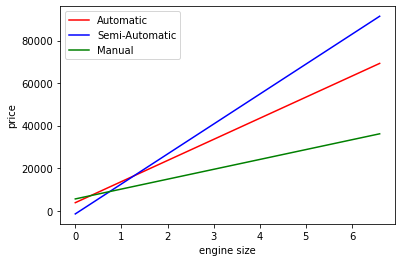
\includegraphics[keepaspectratio]{potential_issue_3_files/figure-pdf/cell-11-output-1.png}}

\begin{Shaded}
\begin{Highlighting}[]
\CommentTok{\# use 3 standard deviation rule to identify outliers}
\NormalTok{outlier\_indices }\OperatorTok{=}\NormalTok{ np.where(np.}\BuiltInTok{abs}\NormalTok{(model.resid) }\OperatorTok{\textgreater{}} \DecValTok{3} \OperatorTok{*}\NormalTok{ model.resid.std())[}\DecValTok{0}\NormalTok{]}
\BuiltInTok{print}\NormalTok{(}\SpecialStringTok{f"Outliers detected at indices: }\SpecialCharTok{\{}\NormalTok{outlier\_indices}\SpecialCharTok{\}}\SpecialStringTok{"}\NormalTok{)}
\end{Highlighting}
\end{Shaded}

\begin{verbatim}
Outliers detected at indices: [ 0  2  3  4 13 15 20 27]
\end{verbatim}

\begin{Shaded}
\begin{Highlighting}[]
\CommentTok{\# {-}{-}{-}{-}{-}{-}{-}{-}{-}{-}{-}{-}{-}{-}{-}{-}{-}{-}{-}{-}{-}{-}{-}{-}{-}{-}{-}{-}{-}{-}{-}{-}{-}{-}{-}{-}{-}{-}{-}{-}{-}{-}}
\CommentTok{\# 2. Identifying High Leverage Points}
\CommentTok{\# {-}{-}{-}{-}{-}{-}{-}{-}{-}{-}{-}{-}{-}{-}{-}{-}{-}{-}{-}{-}{-}{-}{-}{-}{-}{-}{-}{-}{-}{-}{-}{-}{-}{-}{-}{-}{-}{-}{-}{-}{-}{-}}
\CommentTok{\# High leverage points can be detected using the hat matrix (leverage values)}
\NormalTok{leverage }\OperatorTok{=}\NormalTok{ model.get\_influence().hat\_matrix\_diag}
\NormalTok{leverage\_threshold }\OperatorTok{=} \DecValTok{2} \OperatorTok{*}\NormalTok{ (df.shape[}\DecValTok{1}\NormalTok{] }\OperatorTok{/}\NormalTok{ df.shape[}\DecValTok{0}\NormalTok{])  }\CommentTok{\# Common threshold for leverage}
\end{Highlighting}
\end{Shaded}

\subsubsection{Identifying High Leverage
Points}\label{identifying-high-leverage-points}

A common threshold for identifying \textbf{high leverage points} in
regression analysis is:

\(h_i > \frac{2p}{n}\)

where:\\
- \(h_i\) is the leverage value for the ( i )-th observation,\\
- \(p\) is the number of predictors (including the intercept), and\\
- \(n\) is the total number of observations.

\begin{Shaded}
\begin{Highlighting}[]
\CommentTok{\# Plot leverage values}
\NormalTok{plt.figure(figsize}\OperatorTok{=}\NormalTok{(}\DecValTok{10}\NormalTok{, }\DecValTok{6}\NormalTok{))}
\NormalTok{plt.scatter(}\BuiltInTok{range}\NormalTok{(}\BuiltInTok{len}\NormalTok{(leverage)), leverage, alpha}\OperatorTok{=}\FloatTok{0.7}\NormalTok{)}
\NormalTok{plt.axhline(y}\OperatorTok{=}\NormalTok{leverage\_threshold, color}\OperatorTok{=}\StringTok{\textquotesingle{}r\textquotesingle{}}\NormalTok{, linestyle}\OperatorTok{=}\StringTok{\textquotesingle{}{-}{-}\textquotesingle{}}\NormalTok{, label}\OperatorTok{=}\StringTok{\textquotesingle{}Leverage Threshold\textquotesingle{}}\NormalTok{)}
\NormalTok{plt.title(}\StringTok{\textquotesingle{}Leverage Values for High Leverage Points\textquotesingle{}}\NormalTok{)}
\NormalTok{plt.xlabel(}\StringTok{\textquotesingle{}Observation Index\textquotesingle{}}\NormalTok{)}
\NormalTok{plt.ylabel(}\StringTok{\textquotesingle{}Leverage\textquotesingle{}}\NormalTok{)}
\NormalTok{plt.legend()}
\NormalTok{plt.show()}
\end{Highlighting}
\end{Shaded}

\pandocbounded{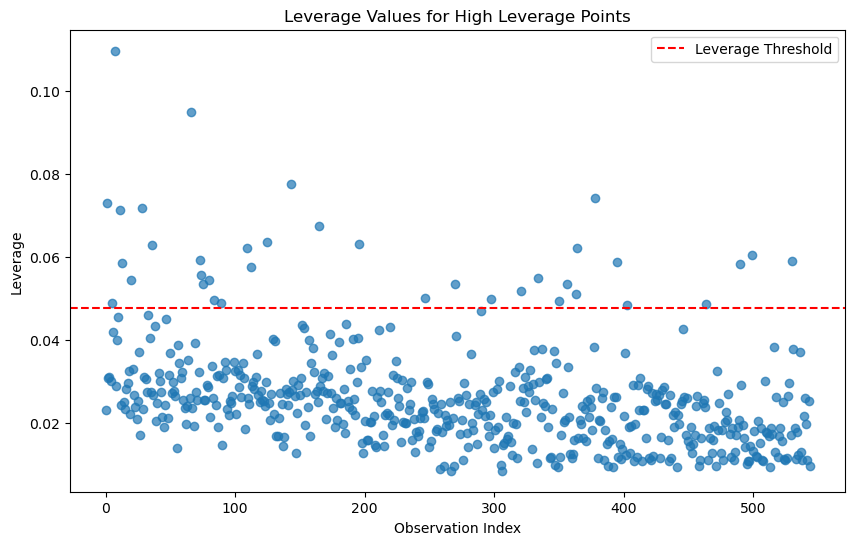
\includegraphics[keepaspectratio]{potential_issue_3_files/figure-pdf/cell-14-output-1.png}}

\begin{Shaded}
\begin{Highlighting}[]
\CommentTok{\# Identify observations with high leverage}
\NormalTok{high\_leverage\_indices }\OperatorTok{=}\NormalTok{ np.where(leverage }\OperatorTok{\textgreater{}}\NormalTok{ leverage\_threshold)[}\DecValTok{0}\NormalTok{]}
\BuiltInTok{print}\NormalTok{(}\SpecialStringTok{f"High leverage points detected at indices: }\SpecialCharTok{\{}\NormalTok{high\_leverage\_indices}\SpecialCharTok{\}}\SpecialStringTok{"}\NormalTok{)}
\end{Highlighting}
\end{Shaded}

\begin{verbatim}
High leverage points detected at indices: [  1   5   7  11  13  20  28  36  66  73  74  75  80  84  89 109 112 125
 143 165 196 247 270 298 321 334 350 356 363 364 378 395 403 464 490 499
 530]
\end{verbatim}

\begin{Shaded}
\begin{Highlighting}[]
\CommentTok{\# {-}{-}{-}{-}{-}{-}{-}{-}{-}{-}{-}{-}{-}{-}{-}{-}{-}{-}{-}{-}{-}{-}{-}{-}{-}{-}{-}{-}{-}{-}{-}{-}{-}{-}{-}{-}{-}{-}{-}{-}{-}{-}}
\CommentTok{\# 3. Cook\textquotesingle{}s Distance for Influential Observations}
\CommentTok{\# {-}{-}{-}{-}{-}{-}{-}{-}{-}{-}{-}{-}{-}{-}{-}{-}{-}{-}{-}{-}{-}{-}{-}{-}{-}{-}{-}{-}{-}{-}{-}{-}{-}{-}{-}{-}{-}{-}{-}{-}{-}{-}}
\CommentTok{\# Cook\textquotesingle{}s distance measures the influence of each observation on the model}
\NormalTok{cooks\_distance }\OperatorTok{=}\NormalTok{ model.get\_influence().cooks\_distance[}\DecValTok{0}\NormalTok{]}

\CommentTok{\# Plot Cook\textquotesingle{}s distance}
\NormalTok{plt.figure(figsize}\OperatorTok{=}\NormalTok{(}\DecValTok{10}\NormalTok{, }\DecValTok{6}\NormalTok{))}
\NormalTok{plt.stem(}\BuiltInTok{range}\NormalTok{(}\BuiltInTok{len}\NormalTok{(cooks\_distance)), cooks\_distance, markerfmt}\OperatorTok{=}\StringTok{","}\NormalTok{)}
\NormalTok{plt.title(}\StringTok{"Cook\textquotesingle{}s Distance for Influential Observations"}\NormalTok{)}
\NormalTok{plt.xlabel(}\StringTok{\textquotesingle{}Observation Index\textquotesingle{}}\NormalTok{)}
\NormalTok{plt.ylabel(}\StringTok{"Cook\textquotesingle{}s Distance"}\NormalTok{)}
\NormalTok{plt.show()}
\end{Highlighting}
\end{Shaded}

\pandocbounded{\includegraphics[keepaspectratio]{potential_issue_3_files/figure-pdf/cell-16-output-1.png}}

Cook's distance is considered high if it is greater than 0.5 and extreme
if it is greater than 1.

\begin{Shaded}
\begin{Highlighting}[]
\CommentTok{\# Identify influential observations}
\NormalTok{influential\_threshold }\OperatorTok{=} \DecValTok{4} \OperatorTok{/}\NormalTok{ (df.shape[}\DecValTok{1}\NormalTok{] }\OperatorTok{{-}} \DecValTok{1}\NormalTok{ ) }\CommentTok{\# Common threshold for Cook\textquotesingle{}s distance}
\NormalTok{influential\_indices }\OperatorTok{=}\NormalTok{ np.where(cooks\_distance }\OperatorTok{\textgreater{}}\NormalTok{ influential\_threshold)[}\DecValTok{0}\NormalTok{]}
\BuiltInTok{print}\NormalTok{(}\SpecialStringTok{f"Influential observations detected at indices: }\SpecialCharTok{\{}\NormalTok{influential\_indices}\SpecialCharTok{\}}\SpecialStringTok{"}\NormalTok{)}
\end{Highlighting}
\end{Shaded}

\begin{verbatim}
Influential observations detected at indices: []
\end{verbatim}

\begin{Shaded}
\begin{Highlighting}[]
\CommentTok{\# =======================================}
\CommentTok{\# 4. Checking Multicollinearity (VIF)}
\CommentTok{\# =======================================}
\CommentTok{\# VIF calculation}
\ImportTok{from}\NormalTok{ statsmodels.stats.outliers\_influence }\ImportTok{import}\NormalTok{ variance\_inflation\_factor}

\KeywordTok{def}\NormalTok{ calculate\_vif(X):}
\NormalTok{    vif\_data }\OperatorTok{=}\NormalTok{ pd.DataFrame()}
\NormalTok{    vif\_data[}\StringTok{"Variable"}\NormalTok{] }\OperatorTok{=}\NormalTok{ X.columns}
\NormalTok{    vif\_data[}\StringTok{"VIF"}\NormalTok{] }\OperatorTok{=}\NormalTok{ [variance\_inflation\_factor(X.values, i) }\ControlFlowTok{for}\NormalTok{ i }\KeywordTok{in} \BuiltInTok{range}\NormalTok{(X.shape[}\DecValTok{1}\NormalTok{])]}
    \ControlFlowTok{return}\NormalTok{ vif\_data}

\NormalTok{X }\OperatorTok{=}\NormalTok{ df[[}\StringTok{\textquotesingle{}area\textquotesingle{}}\NormalTok{, }\StringTok{\textquotesingle{}bedrooms\textquotesingle{}}\NormalTok{, }\StringTok{\textquotesingle{}bathrooms\textquotesingle{}}\NormalTok{, }\StringTok{\textquotesingle{}stories\textquotesingle{}}\NormalTok{, }\StringTok{\textquotesingle{}mainroad\textquotesingle{}}\NormalTok{, }\StringTok{\textquotesingle{}guestroom\textquotesingle{}}\NormalTok{, }\StringTok{\textquotesingle{}basement\textquotesingle{}}\NormalTok{, }\StringTok{\textquotesingle{}hotwaterheating\textquotesingle{}}\NormalTok{, }\StringTok{\textquotesingle{}airconditioning\textquotesingle{}}\NormalTok{, }\StringTok{\textquotesingle{}parking\textquotesingle{}}\NormalTok{, }\StringTok{\textquotesingle{}prefarea\textquotesingle{}}\NormalTok{, }\StringTok{\textquotesingle{}furnishingstatus\textquotesingle{}}\NormalTok{]]}

\CommentTok{\# one{-}hot encoding for categorical variables}
\NormalTok{X }\OperatorTok{=}\NormalTok{ pd.get\_dummies(X, drop\_first}\OperatorTok{=}\VariableTok{True}\NormalTok{, dtype}\OperatorTok{=}\BuiltInTok{float}\NormalTok{)}


\NormalTok{vif\_data }\OperatorTok{=}\NormalTok{ calculate\_vif(X)}
\BuiltInTok{print}\NormalTok{(}\StringTok{"}\CharTok{\textbackslash{}n}\StringTok{Variance Inflation Factors:"}\NormalTok{)}
\BuiltInTok{print}\NormalTok{(vif\_data.sort\_values(}\StringTok{\textquotesingle{}VIF\textquotesingle{}}\NormalTok{, ascending}\OperatorTok{=}\VariableTok{False}\NormalTok{))}
\end{Highlighting}
\end{Shaded}

\begin{verbatim}

Variance Inflation Factors:
                           Variable        VIF
1                          bedrooms  16.652387
2                         bathrooms   9.417643
0                              area   8.276447
3                           stories   7.880730
5                      mainroad_yes   6.884806
11  furnishingstatus_semi-furnished   2.386831
7                      basement_yes   2.019858
12     furnishingstatus_unfurnished   2.008632
4                           parking   1.986400
9               airconditioning_yes   1.767753
10                     prefarea_yes   1.494211
6                     guestroom_yes   1.473234
8               hotwaterheating_yes   1.091568
\end{verbatim}

\begin{Shaded}
\begin{Highlighting}[]
\CommentTok{\# Rule of thumb: VIF \textgreater{} 10 indicates significant multicollinearity}
\NormalTok{multicollinear\_features }\OperatorTok{=}\NormalTok{ vif\_data[vif\_data[}\StringTok{\textquotesingle{}VIF\textquotesingle{}}\NormalTok{] }\OperatorTok{\textgreater{}} \DecValTok{10}\NormalTok{][}\StringTok{\textquotesingle{}Variable\textquotesingle{}}\NormalTok{]}
\BuiltInTok{print}\NormalTok{(}\SpecialStringTok{f"Features with significant multicollinearity: }\SpecialCharTok{\{}\NormalTok{multicollinear\_features}\SpecialCharTok{.}\NormalTok{tolist()}\SpecialCharTok{\}}\SpecialStringTok{"}\NormalTok{)}
\end{Highlighting}
\end{Shaded}

\begin{verbatim}
Features with significant multicollinearity: ['bedrooms']
\end{verbatim}

\begin{Shaded}
\begin{Highlighting}[]
\CommentTok{\# =======================================}
\CommentTok{\# 4. Checking Multicollinearity (Correlation Matrix)}
\CommentTok{\# =======================================}
\CommentTok{\# Correlation matrix}
\NormalTok{correlation\_matrix }\OperatorTok{=}\NormalTok{ X.corr()}
\NormalTok{plt.figure(figsize}\OperatorTok{=}\NormalTok{(}\DecValTok{8}\NormalTok{, }\DecValTok{6}\NormalTok{))}
\NormalTok{sns.heatmap(correlation\_matrix, annot}\OperatorTok{=}\VariableTok{True}\NormalTok{, cmap}\OperatorTok{=}\StringTok{\textquotesingle{}coolwarm\textquotesingle{}}\NormalTok{)}
\NormalTok{plt.title(}\StringTok{\textquotesingle{}Correlation Matrix\textquotesingle{}}\NormalTok{)}\OperatorTok{;}
\end{Highlighting}
\end{Shaded}

\pandocbounded{\includegraphics[keepaspectratio]{potential_issue_3_files/figure-pdf/cell-20-output-1.png}}

\begin{Shaded}
\begin{Highlighting}[]
\CommentTok{\#output the correlation of other predictors with the bedrooms}
\NormalTok{X.corr()[}\StringTok{\textquotesingle{}bedrooms\textquotesingle{}}\NormalTok{].}\BuiltInTok{abs}\NormalTok{().sort\_values(ascending}\OperatorTok{=}\VariableTok{False}\NormalTok{)}
\end{Highlighting}
\end{Shaded}

\begin{verbatim}
bedrooms                           1.000000
stories                            0.408564
bathrooms                          0.373930
airconditioning_yes                0.160603
area                               0.151858
parking                            0.139270
furnishingstatus_unfurnished       0.126252
basement_yes                       0.097312
guestroom_yes                      0.080549
prefarea_yes                       0.079023
furnishingstatus_semi-furnished    0.050040
hotwaterheating_yes                0.046049
mainroad_yes                       0.012033
Name: bedrooms, dtype: float64
\end{verbatim}

\begin{Shaded}
\begin{Highlighting}[]
\CommentTok{\# {-}{-}{-}{-}{-}{-}{-}{-}{-}{-}{-}{-}{-}{-}{-}{-}{-}{-}{-}{-}{-}{-}{-}{-}{-}{-}{-}{-}{-}{-}{-}{-}{-}{-}{-}{-}{-}{-}{-}{-}{-}{-}}
\CommentTok{\# 5. Analyzing Residual Patterns}
\CommentTok{\# {-}{-}{-}{-}{-}{-}{-}{-}{-}{-}{-}{-}{-}{-}{-}{-}{-}{-}{-}{-}{-}{-}{-}{-}{-}{-}{-}{-}{-}{-}{-}{-}{-}{-}{-}{-}{-}{-}{-}{-}{-}{-}}
\CommentTok{\# Residuals vs Fitted Values Plot}
\NormalTok{fitted\_values }\OperatorTok{=}\NormalTok{ model.fittedvalues}
\NormalTok{residuals }\OperatorTok{=}\NormalTok{ model.resid}

\NormalTok{plt.figure(figsize}\OperatorTok{=}\NormalTok{(}\DecValTok{10}\NormalTok{, }\DecValTok{6}\NormalTok{))}
\NormalTok{sns.residplot(x}\OperatorTok{=}\NormalTok{fitted\_values, y}\OperatorTok{=}\NormalTok{residuals, lowess}\OperatorTok{=}\VariableTok{True}\NormalTok{, line\_kws}\OperatorTok{=}\NormalTok{\{}\StringTok{\textquotesingle{}color\textquotesingle{}}\NormalTok{: }\StringTok{\textquotesingle{}red\textquotesingle{}}\NormalTok{, }\StringTok{\textquotesingle{}lw\textquotesingle{}}\NormalTok{: }\DecValTok{1}\NormalTok{\})}
\NormalTok{plt.title(}\StringTok{\textquotesingle{}Residuals vs Fitted Values\textquotesingle{}}\NormalTok{)}
\NormalTok{plt.xlabel(}\StringTok{\textquotesingle{}Fitted Values\textquotesingle{}}\NormalTok{)}
\NormalTok{plt.ylabel(}\StringTok{\textquotesingle{}Residuals\textquotesingle{}}\NormalTok{)}\OperatorTok{;}

\CommentTok{\# QQ Plot for Normality of Residuals}
\NormalTok{plt.figure(figsize}\OperatorTok{=}\NormalTok{(}\DecValTok{10}\NormalTok{, }\DecValTok{6}\NormalTok{))}
\NormalTok{sm.qqplot(residuals, line}\OperatorTok{=}\StringTok{\textquotesingle{}s\textquotesingle{}}\NormalTok{)}
\NormalTok{plt.title(}\StringTok{\textquotesingle{}QQ Plot of Residuals\textquotesingle{}}\NormalTok{)}\OperatorTok{;}
\end{Highlighting}
\end{Shaded}

\pandocbounded{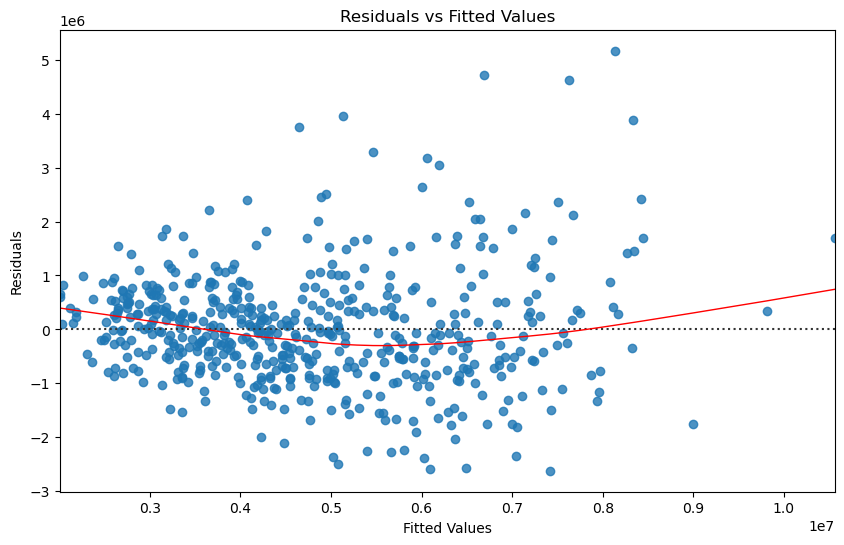
\includegraphics[keepaspectratio]{potential_issue_3_files/figure-pdf/cell-22-output-1.png}}

\begin{verbatim}
<Figure size 1000x600 with 0 Axes>
\end{verbatim}

\pandocbounded{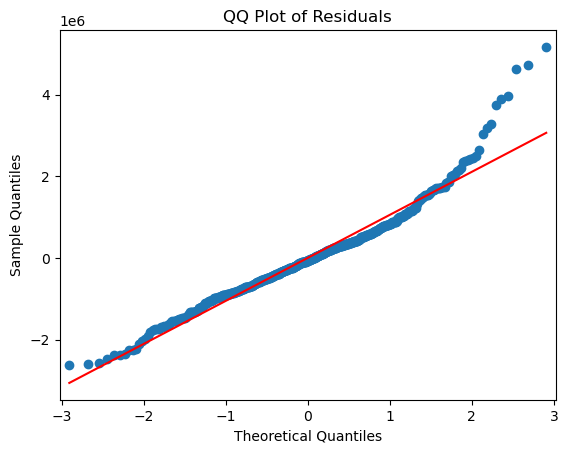
\includegraphics[keepaspectratio]{potential_issue_3_files/figure-pdf/cell-22-output-3.png}}

\begin{Shaded}
\begin{Highlighting}[]
\NormalTok{plt.figure(figsize}\OperatorTok{=}\NormalTok{(}\DecValTok{8}\NormalTok{, }\DecValTok{5}\NormalTok{))}
\NormalTok{sns.histplot(residuals, kde}\OperatorTok{=}\VariableTok{True}\NormalTok{, bins}\OperatorTok{=}\DecValTok{20}\NormalTok{)}
\NormalTok{plt.axvline(residuals.mean(), color}\OperatorTok{=}\StringTok{\textquotesingle{}red\textquotesingle{}}\NormalTok{, linestyle}\OperatorTok{=}\StringTok{\textquotesingle{}{-}{-}\textquotesingle{}}\NormalTok{, label}\OperatorTok{=}\StringTok{"Mean Residual"}\NormalTok{)}
\NormalTok{plt.xlabel(}\StringTok{"Residuals"}\NormalTok{)}
\NormalTok{plt.ylabel(}\StringTok{"Density"}\NormalTok{)}
\NormalTok{plt.title(}\StringTok{"Histogram of Residuals"}\NormalTok{)}
\NormalTok{plt.legend()}
\NormalTok{plt.show()}
\end{Highlighting}
\end{Shaded}

\pandocbounded{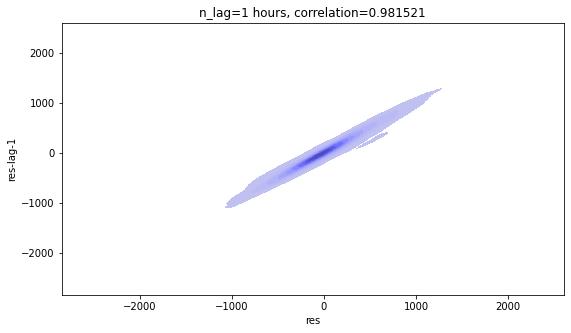
\includegraphics[keepaspectratio]{potential_issue_3_files/figure-pdf/cell-23-output-1.png}}

\bookmarksetup{startatroot}

\chapter{Beyond Fit (statistical
theory)}\label{beyond-fit-statistical-theory}

\emph{Read section 3.3.3 (4, 5, \& 6) of the book before using these
notes.}

\emph{Note that in this course, lecture notes are not sufficient, you
must read the book for better understanding. Lecture notes are just
implementing the concepts of the book on a dataset, but not explaining
the concepts elaborately.}

Let us continue with the car price prediction example from the previous
chapter.

\begin{Shaded}
\begin{Highlighting}[]
\ImportTok{import}\NormalTok{ pandas }\ImportTok{as}\NormalTok{ pd}
\ImportTok{import}\NormalTok{ numpy }\ImportTok{as}\NormalTok{ np}
\ImportTok{import}\NormalTok{ statsmodels.formula.api }\ImportTok{as}\NormalTok{ smf}
\ImportTok{import}\NormalTok{ seaborn }\ImportTok{as}\NormalTok{ sns}
\ImportTok{import}\NormalTok{ matplotlib.pyplot }\ImportTok{as}\NormalTok{ plt}
\ImportTok{import}\NormalTok{ statsmodels.api }\ImportTok{as}\NormalTok{ sm}
\ImportTok{from}\NormalTok{ scipy }\ImportTok{import}\NormalTok{ stats}
\ImportTok{from}\NormalTok{ sklearn.model\_selection }\ImportTok{import}\NormalTok{ cross\_val\_predict}
\ImportTok{from}\NormalTok{ patsy }\ImportTok{import}\NormalTok{ dmatrices}
\ImportTok{from}\NormalTok{ sklearn.linear\_model }\ImportTok{import}\NormalTok{ LinearRegression}
\ImportTok{from}\NormalTok{ sklearn.metrics }\ImportTok{import}\NormalTok{ mean\_squared\_error}
\end{Highlighting}
\end{Shaded}

\begin{Shaded}
\begin{Highlighting}[]
\NormalTok{trainf }\OperatorTok{=}\NormalTok{ pd.read\_csv(}\StringTok{\textquotesingle{}./Datasets/Car\_features\_train.csv\textquotesingle{}}\NormalTok{)}
\NormalTok{trainp }\OperatorTok{=}\NormalTok{ pd.read\_csv(}\StringTok{\textquotesingle{}./Datasets/Car\_prices\_train.csv\textquotesingle{}}\NormalTok{)}
\NormalTok{testf }\OperatorTok{=}\NormalTok{ pd.read\_csv(}\StringTok{\textquotesingle{}./Datasets/Car\_features\_test.csv\textquotesingle{}}\NormalTok{)}
\NormalTok{testp }\OperatorTok{=}\NormalTok{ pd.read\_csv(}\StringTok{\textquotesingle{}./Datasets/Car\_prices\_test.csv\textquotesingle{}}\NormalTok{)}
\NormalTok{train }\OperatorTok{=}\NormalTok{ pd.merge(trainf,trainp)}
\NormalTok{train.head()}
\end{Highlighting}
\end{Shaded}

\begin{longtable}[]{@{}llllllllllll@{}}
\toprule\noalign{}
& carID & brand & model & year & transmission & mileage & fuelType & tax
& mpg & engineSize & price \\
\midrule\noalign{}
\endhead
\bottomrule\noalign{}
\endlastfoot
0 & 18473 & bmw & 6 Series & 2020 & Semi-Auto & 11 & Diesel & 145 &
53.3282 & 3.0 & 37980 \\
1 & 15064 & bmw & 6 Series & 2019 & Semi-Auto & 10813 & Diesel & 145 &
53.0430 & 3.0 & 33980 \\
2 & 18268 & bmw & 6 Series & 2020 & Semi-Auto & 6 & Diesel & 145 &
53.4379 & 3.0 & 36850 \\
3 & 18480 & bmw & 6 Series & 2017 & Semi-Auto & 18895 & Diesel & 145 &
51.5140 & 3.0 & 25998 \\
4 & 18492 & bmw & 6 Series & 2015 & Automatic & 62953 & Diesel & 160 &
51.4903 & 3.0 & 18990 \\
\end{longtable}

\begin{Shaded}
\begin{Highlighting}[]
\CommentTok{\# Considering the model developed to address assumptions in the previous chapter}
\CommentTok{\# Model with an interaction term and a variable transformation term}
\NormalTok{ols\_object }\OperatorTok{=}\NormalTok{ smf.ols(formula }\OperatorTok{=} \StringTok{\textquotesingle{}np.log(price)\textasciitilde{}(year+engineSize+mileage+mpg)**2+I(mileage**2)\textquotesingle{}}\NormalTok{, data }\OperatorTok{=}\NormalTok{ train)}
\NormalTok{model\_log }\OperatorTok{=}\NormalTok{ ols\_object.fit()}
\NormalTok{model\_log.summary()}
\end{Highlighting}
\end{Shaded}

\begin{center}
\begin{tabular}{lclc}
\toprule
\textbf{Dep. Variable:}     &  np.log(price)   & \textbf{  R-squared:         } &     0.803   \\
\textbf{Model:}             &       OLS        & \textbf{  Adj. R-squared:    } &     0.803   \\
\textbf{Method:}            &  Least Squares   & \textbf{  F-statistic:       } &     1834.   \\
\textbf{Date:}              & Sun, 10 Mar 2024 & \textbf{  Prob (F-statistic):} &     0.00    \\
\textbf{Time:}              &     16:51:01     & \textbf{  Log-Likelihood:    } &   -1173.8   \\
\textbf{No. Observations:}  &        4960      & \textbf{  AIC:               } &     2372.   \\
\textbf{Df Residuals:}      &        4948      & \textbf{  BIC:               } &     2450.   \\
\textbf{Df Model:}          &          11      & \textbf{                     } &             \\
\textbf{Covariance Type:}   &    nonrobust     & \textbf{                     } &             \\
\bottomrule
\end{tabular}
\begin{tabular}{lcccccc}
                            & \textbf{coef} & \textbf{std err} & \textbf{t} & \textbf{P$> |$t$|$} & \textbf{[0.025} & \textbf{0.975]}  \\
\midrule
\textbf{Intercept}          &    -238.2125  &       25.790     &    -9.237  &         0.000        &     -288.773    &     -187.652     \\
\textbf{year}               &       0.1227  &        0.013     &     9.608  &         0.000        &        0.098    &        0.148     \\
\textbf{engineSize}         &      13.8349  &        5.795     &     2.387  &         0.017        &        2.475    &       25.195     \\
\textbf{mileage}            &       0.0005  &        0.000     &     3.837  &         0.000        &        0.000    &        0.001     \\
\textbf{mpg}                &      -1.2446  &        0.345     &    -3.610  &         0.000        &       -1.921    &       -0.569     \\
\textbf{year:engineSize}    &      -0.0067  &        0.003     &    -2.324  &         0.020        &       -0.012    &       -0.001     \\
\textbf{year:mileage}       &    -2.67e-07  &      6.8e-08     &    -3.923  &         0.000        &       -4e-07    &    -1.34e-07     \\
\textbf{year:mpg}           &       0.0006  &        0.000     &     3.591  &         0.000        &        0.000    &        0.001     \\
\textbf{engineSize:mileage} &   -2.668e-07  &     4.08e-07     &    -0.654  &         0.513        &    -1.07e-06    &     5.33e-07     \\
\textbf{engineSize:mpg}     &       0.0028  &        0.000     &     6.842  &         0.000        &        0.002    &        0.004     \\
\textbf{mileage:mpg}        &    7.235e-08  &     1.79e-08     &     4.036  &         0.000        &     3.72e-08    &     1.08e-07     \\
\textbf{I(mileage ** 2)}    &    1.828e-11  &     5.64e-12     &     3.240  &         0.001        &     7.22e-12    &     2.93e-11     \\
\bottomrule
\end{tabular}
\begin{tabular}{lclc}
\textbf{Omnibus:}       & 711.514 & \textbf{  Durbin-Watson:     } &    0.498  \\
\textbf{Prob(Omnibus):} &   0.000 & \textbf{  Jarque-Bera (JB):  } & 2545.807  \\
\textbf{Skew:}          &   0.699 & \textbf{  Prob(JB):          } &     0.00  \\
\textbf{Kurtosis:}      &   6.220 & \textbf{  Cond. No.          } & 1.73e+13  \\
\bottomrule
\end{tabular}
%\caption{OLS Regression Results}
\end{center}

Notes: \newline
 [1] Standard Errors assume that the covariance matrix of the errors is correctly specified. \newline
 [2] The condition number is large, 1.73e+13. This might indicate that there are \newline
 strong multicollinearity or other numerical problems.

\begin{Shaded}
\begin{Highlighting}[]
\CommentTok{\#Computing RMSE on test data}
\NormalTok{pred\_price\_log }\OperatorTok{=}\NormalTok{ model\_log.predict(testf)}
\NormalTok{np.sqrt(((testp.price }\OperatorTok{{-}}\NormalTok{ np.exp(pred\_price\_log))}\OperatorTok{**}\DecValTok{2}\NormalTok{).mean())}
\end{Highlighting}
\end{Shaded}

\begin{verbatim}
9094.209473232966
\end{verbatim}

\section{Outliers}\label{outliers}

An outlier is a point for which the true response (\(y_i\)) is far from
the value predicted by the model. Residual plots can be used to identify
outliers.

If the the response at the \(i^{th}\) observation is \(y_i\), the
prediction is \(\hat{y}_i\), then the residual \(e_i\) is:

\[e_i = y_i - \hat{y_i}\]

\begin{Shaded}
\begin{Highlighting}[]
\CommentTok{\#Plotting residuals vs fitted values}
\NormalTok{sns.}\BuiltInTok{set}\NormalTok{(rc}\OperatorTok{=}\NormalTok{\{}\StringTok{\textquotesingle{}figure.figsize\textquotesingle{}}\NormalTok{:(}\DecValTok{10}\NormalTok{,}\DecValTok{6}\NormalTok{)\})}
\NormalTok{sns.scatterplot(x }\OperatorTok{=}\NormalTok{ (model\_log.fittedvalues), y}\OperatorTok{=}\NormalTok{(model\_log.resid),color }\OperatorTok{=} \StringTok{\textquotesingle{}orange\textquotesingle{}}\NormalTok{)}
\NormalTok{sns.lineplot(x }\OperatorTok{=}\NormalTok{ [model\_log.fittedvalues.}\BuiltInTok{min}\NormalTok{(),model\_log.fittedvalues.}\BuiltInTok{max}\NormalTok{()],y }\OperatorTok{=}\NormalTok{ [}\DecValTok{0}\NormalTok{,}\DecValTok{0}\NormalTok{],color }\OperatorTok{=} \StringTok{\textquotesingle{}blue\textquotesingle{}}\NormalTok{)}
\NormalTok{plt.xlabel(}\StringTok{\textquotesingle{}Fitted values\textquotesingle{}}\NormalTok{)}
\NormalTok{plt.ylabel(}\StringTok{\textquotesingle{}Residuals\textquotesingle{}}\NormalTok{)}\OperatorTok{;}
\end{Highlighting}
\end{Shaded}

\pandocbounded{\includegraphics[keepaspectratio]{Lec5_Potential_issues_files/figure-pdf/cell-6-output-1.png}}

Some of the errors may be high. However, it is difficult to decide how
large a residual needs to be before we can consider a point to be an
outlier. To address this problem, we have standardized residuals, which
are defined as:

\[r_i = \frac{e_i}{RSE(\sqrt{1-h_{ii}})},\] where \(r_i\) is the
standardized residual, \(RSE\) is the residual standard error, and
\(h_{ii}\) is the leverage \emph{(introduced in the next section)} of
the \(i^{th}\) observation.

Standardized residuals, allow the residuals to be compared on a
\emph{standard scale}.

\textbf{Issue with standardized residuals:}, If the observation
corresponding to the standardized residual has a high leverage, then it
will drag the regression line / plane / hyperplane towards it, thereby
influencing the estimate of the residual itself.

\textbf{Studentized residuals:} To address the issue with standardized
residuals, studentized residual for the \(i^{th}\) observation is
computed as the standardized residual, but with the \(RSE\) (residual
standard error) computed after removing the \(i^{th}\) observation from
the data. Studentized residual, \(t_i\) for the \(i^{th}\) observation
is given as:

\[t_i = \frac{e_i}{RSE_{i}(\sqrt{1-h_{ii}})},\] where \(RSE_{i}\) is the
residual standard error of the model developed on the data without the
\(i^{th}\) observation.

\textbf{Distribution of studentized residuals:} If the regression model
is appropriate such that no case is outlying because of a change in the
model, then each studentized residual will follow a \(t\) distribution
with \((n–p–1)\) degrees of freedom.

As the studentized residuals follow a \(t\) distribution, we can conduct
a hypothesis test to identify whether an observation is an outlier or
not for a given sigificance level. Note that the test will be two-sided
since we are not concerned with the sign of the residuals, but only
their absolute values.

In the current example, for a signficance level of 5\%, the critical
\(t\)-statistic is \(t\big(1 - \frac{\alpha}{2}, n - p - 1\big)\), as
calculated below.

\begin{Shaded}
\begin{Highlighting}[]
\NormalTok{n }\OperatorTok{=}\NormalTok{ train.shape[}\DecValTok{0}\NormalTok{]}
\NormalTok{p }\OperatorTok{=}\NormalTok{ model\_log.df\_model}
\NormalTok{alpha }\OperatorTok{=} \FloatTok{0.05}

\CommentTok{\# Critical value}
\NormalTok{stats.t.ppf(}\DecValTok{1} \OperatorTok{{-}}\NormalTok{ alpha}\OperatorTok{/}\DecValTok{2}\NormalTok{, n }\OperatorTok{{-}}\NormalTok{ p }\OperatorTok{{-}} \DecValTok{1}\NormalTok{)}
\end{Highlighting}
\end{Shaded}

\begin{verbatim}
1.9604435402730618
\end{verbatim}

If we were conducting the test for a single observation, we'll compare
the studentized residual for that observation with the critical
\(t\)-statistic, and if the residual is greater than the critical value,
we'll consider that observation as an outlier.

However, typically, we'll be interested in conducting this test for all
observations, and thus we'll need a more conservative critical value for
the same signficance level. This critical value is given by the
Bonferroni correction as
\(t\big(1 - \frac{\alpha}{2n}, n - p - 1\big)\).

Thus, the minimum value of studentized residual for which the
observation will be classified as an outlier is:

\begin{Shaded}
\begin{Highlighting}[]
\NormalTok{critical\_value }\OperatorTok{=}\NormalTok{ stats.t.ppf(}\DecValTok{1}\OperatorTok{{-}}\NormalTok{alpha}\OperatorTok{/}\NormalTok{(}\DecValTok{2}\OperatorTok{*}\NormalTok{n), n }\OperatorTok{{-}}\NormalTok{ p }\OperatorTok{{-}} \DecValTok{1}\NormalTok{)}
\NormalTok{critical\_value}
\end{Highlighting}
\end{Shaded}

\begin{verbatim}
4.4200129981725365
\end{verbatim}

The studentized residuals can be obtained using the
\texttt{outlier\_test()} method of the object returned by the
\texttt{fit()} method of an OLS object. Let us find the studentized
residuals in our car \texttt{price} prediction model.

\begin{Shaded}
\begin{Highlighting}[]
\CommentTok{\#Studentized residuals}
\NormalTok{out }\OperatorTok{=}\NormalTok{ model\_log.outlier\_test()}
\NormalTok{out}
\end{Highlighting}
\end{Shaded}

\begin{longtable}[]{@{}llll@{}}
\toprule\noalign{}
& student\_resid & unadj\_p & bonf(p) \\
\midrule\noalign{}
\endhead
\bottomrule\noalign{}
\endlastfoot
0 & -1.164204 & 0.244398 & 1.0 \\
1 & -0.801879 & 0.422661 & 1.0 \\
2 & -1.263820 & 0.206354 & 1.0 \\
3 & -0.614171 & 0.539131 & 1.0 \\
4 & 0.027929 & 0.977720 & 1.0 \\
... & ... & ... & ... \\
4955 & -0.523361 & 0.600747 & 1.0 \\
4956 & -0.509538 & 0.610398 & 1.0 \\
4957 & -1.718808 & 0.085712 & 1.0 \\
4958 & -0.077594 & 0.938154 & 1.0 \\
4959 & -0.482388 & 0.629551 & 1.0 \\
\end{longtable}

Studentized residuals are in the first column of the above table. Let us
plot the studentized residuals against fitted values. In the figure
below, the studentized residuals above the top dotted green line and
below the bottom dotted green line are outliers.

\begin{Shaded}
\begin{Highlighting}[]
\CommentTok{\#Plotting studentized residuals vs fitted values}
\NormalTok{sns.scatterplot(x }\OperatorTok{=}\NormalTok{ (model\_log.fittedvalues), y}\OperatorTok{=}\NormalTok{(out.student\_resid),color }\OperatorTok{=} \StringTok{\textquotesingle{}orange\textquotesingle{}}\NormalTok{)}
\NormalTok{sns.lineplot(x }\OperatorTok{=}\NormalTok{ [model\_log.fittedvalues.}\BuiltInTok{min}\NormalTok{(),model\_log.fittedvalues.}\BuiltInTok{max}\NormalTok{()],y }\OperatorTok{=}\NormalTok{ [}\DecValTok{0}\NormalTok{,}\DecValTok{0}\NormalTok{],color }\OperatorTok{=} \StringTok{\textquotesingle{}blue\textquotesingle{}}\NormalTok{)}
\NormalTok{ax }\OperatorTok{=}\NormalTok{ sns.lineplot(x }\OperatorTok{=}\NormalTok{ [model\_log.fittedvalues.}\BuiltInTok{min}\NormalTok{(),model\_log.fittedvalues.}\BuiltInTok{max}\NormalTok{()],y }\OperatorTok{=}\NormalTok{ [critical\_value, critical\_value],}
\NormalTok{             color }\OperatorTok{=} \StringTok{\textquotesingle{}green\textquotesingle{}}\NormalTok{)}
\NormalTok{sns.lineplot(x }\OperatorTok{=}\NormalTok{ [model\_log.fittedvalues.}\BuiltInTok{min}\NormalTok{(),model\_log.fittedvalues.}\BuiltInTok{max}\NormalTok{()],y }\OperatorTok{=}\NormalTok{ [}\OperatorTok{{-}}\NormalTok{critical\_value, }\OperatorTok{{-}}\NormalTok{critical\_value],}
\NormalTok{             color }\OperatorTok{=} \StringTok{\textquotesingle{}green\textquotesingle{}}\NormalTok{)}
\NormalTok{ax.lines[}\DecValTok{1}\NormalTok{].set\_linestyle(}\StringTok{"{-}{-}"}\NormalTok{)}
\NormalTok{ax.lines[}\DecValTok{2}\NormalTok{].set\_linestyle(}\StringTok{"{-}{-}"}\NormalTok{)}

\NormalTok{plt.xlabel(}\StringTok{\textquotesingle{}Fitted values\textquotesingle{}}\NormalTok{)}
\NormalTok{plt.ylabel(}\StringTok{\textquotesingle{}Studentized Residuals\textquotesingle{}}\NormalTok{)}\OperatorTok{;}
\end{Highlighting}
\end{Shaded}

\pandocbounded{\includegraphics[keepaspectratio]{Lec5_Potential_issues_files/figure-pdf/cell-10-output-1.png}}

\textbf{Outliers:} Observations whose studentized residuals have a
magnitude greater than \(t\big(1 - \frac{\alpha}{2n}, n - p - 1\big)\).

\textbf{Impact of outliers:} Outliers do not have a large impact on the
OLS line / plane / hyperplane as long as they don't have a high leverage
\emph{(discussed in the next section)}. However, outliers do inflate the
residual standard error (RSE). RSE in turn is used to compute the
standard errors of regression coefficients. As a result, statistically
significant variables may appear to be insignificant, and \(R^2\) may
appear to be lower.

\textbf{Are there outliers in our example?}

\begin{Shaded}
\begin{Highlighting}[]
\CommentTok{\#Number of points with absolute studentized residuals greater than critical\_value}
\NormalTok{np.}\BuiltInTok{sum}\NormalTok{(np.}\BuiltInTok{abs}\NormalTok{(out.student\_resid) }\OperatorTok{\textgreater{}}\NormalTok{ critical\_value)}
\end{Highlighting}
\end{Shaded}

\begin{verbatim}
19
\end{verbatim}

Let us analyze the outliers.

\begin{Shaded}
\begin{Highlighting}[]
\NormalTok{ind }\OperatorTok{=}\NormalTok{ (np.}\BuiltInTok{abs}\NormalTok{(out.student\_resid) }\OperatorTok{\textgreater{}}\NormalTok{ critical\_value)}
\NormalTok{pd.concat([train.loc[ind,:], np.exp(model\_log.fittedvalues[ind])], axis }\OperatorTok{=} \DecValTok{1}\NormalTok{)}
\end{Highlighting}
\end{Shaded}

\begin{longtable}[]{@{}lllllllllllll@{}}
\toprule\noalign{}
& carID & brand & model & year & transmission & mileage & fuelType & tax
& mpg & engineSize & price & 0 \\
\midrule\noalign{}
\endhead
\bottomrule\noalign{}
\endlastfoot
2042 & 18228 & bmw & i3 & 2017 & Automatic & 24041 & Hybrid & 0 &
78.2726 & 0.0 & 21495 & 5537.337460 \\
2046 & 17362 & bmw & i3 & 2016 & Automatic & 68000 & Hybrid & 0 &
78.0258 & 0.0 & 15990 & 4107.811771 \\
2050 & 19224 & bmw & i3 & 2016 & Automatic & 20013 & Hybrid & 0 &
77.9310 & 0.0 & 19875 & 4784.986021 \\
2051 & 13913 & bmw & i3 & 2014 & Automatic & 34539 & Hybrid & 0 &
78.3838 & 0.0 & 14495 & 3269.686113 \\
2055 & 16512 & bmw & i3 & 2017 & Automatic & 28169 & Hybrid & 0 &
77.9799 & 0.0 & 23751 & 5454.207333 \\
2059 & 15844 & bmw & i3 & 2016 & Automatic & 19995 & Hybrid & 0 &
78.2825 & 0.0 & 19850 & 4773.707307 \\
2060 & 12107 & bmw & i3 & 2016 & Automatic & 8421 & Hybrid & 0 & 77.9125
& 0.0 & 19490 & 5028.048305 \\
2061 & 18215 & bmw & i3 & 2014 & Automatic & 37161 & Hybrid & 0 &
77.7505 & 0.0 & 14182 & 3259.101789 \\
2063 & 15617 & bmw & i3 & 2017 & Automatic & 41949 & Hybrid & 140 &
78.1907 & 0.0 & 19998 & 5173.402125 \\
2064 & 18020 & bmw & i3 & 2015 & Automatic & 9886 & Hybrid & 0 & 78.1810
& 0.0 & 17481 & 4214.053932 \\
2143 & 12972 & bmw & i8 & 2017 & Automatic & 9992 & Hybrid & 135 &
69.2767 & 1.5 & 59950 & 14675.519883 \\
2144 & 13826 & bmw & i8 & 2015 & Automatic & 43323 & Hybrid & 0 &
69.2683 & 1.5 & 44990 & 9289.744847 \\
2150 & 18949 & bmw & i8 & 2015 & Automatic & 43102 & Hybrid & 0 &
69.0922 & 1.5 & 42890 & 9300.576839 \\
2151 & 18977 & bmw & i8 & 2016 & Automatic & 10087 & Hybrid & 0 &
68.9279 & 1.5 & 48998 & 12607.867130 \\
2744 & 18866 & merc & M Class & 2004 & Automatic & 121000 & Diesel & 325
& 29.3713 & 2.7 & 19950 & 4068.883513 \\
3548 & 13149 & audi & S4 & 2019 & Automatic & 4900 & Diesel & 145 &
40.7030 & 0.0 & 45000 & 10679.644966 \\
4116 & 16420 & audi & SQ5 & 2020 & Automatic & 1500 & Diesel & 145 &
34.7968 & 0.0 & 56450 & 13166.374034 \\
4117 & 17611 & audi & SQ5 & 2019 & Automatic & 1500 & Diesel & 145 &
34.5016 & 0.0 & 48800 & 11426.005642 \\
4851 & 16577 & bmw & Z3 & 2002 & Automatic & 16500 & Petrol & 325 &
29.7614 & 2.2 & 14995 & 3426.196256 \\
\end{longtable}

\textbf{Do you notice some unique characteristics of these observations
due to which they may be outliers?}

\textbf{What methods you can propose to estimate the price of these
outliers more accurately, which will also result in the overall
reduction in RMSE?}

\section{High leverage points}\label{high-leverage-points}

High leverage points are those with an unsual value of the predictor(s).
They have the potential to have a relatively higher impact on the OLS
line / plane / hyperplane, as compared to the outliers.

\textbf{Leverage statistic} (page 99 of the book): In order to quantify
an observation's leverage, we compute the leverage statistic. A large
value of this statistic indicates an observation with high leverage. For
simple linear regression, \begin{equation}
h_i = \frac{1}{n} + \frac{(x_i - \bar x)^2}{\sum_{i'=1}^{n}(x_{i'} - \bar x)^2}.
\end{equation}

It is clear from this equation that \(h_i\) increases with the distance
of \(x_i\) from \(\bar x\). A large value of \(h_i\) indicates that the
\(i^{th}\) observation is distance from the center of all the other
observations in terms of predictor values.

The leverage statistic \(h_i\) is always between \(1/n\) and \(1\), and
the average leverage for all the observations is always equal to
\((p+1)/n\):

\begin{equation}
\bar{h} = \frac{p+1}{n}
\end{equation}

So if a given observation has a leverage statistic that greatly exceeds
\((p+1)/n\), then we may suspect that the corresponding point has high
leverage.

If the \(i^{th}\) observation has a large leverage \(h_i\), it may
exercise substantial leverage in determining the fitted value
\(\hat{Y}_i\), because:

\begin{itemize}
\item
  The fitted value \(\hat{Y}_i\) is a linear combination of the observed
  \(Y\) values, and \(h_i\) is the weight of observation \(Y_i\) in
  determining this fitted value.
\item
  The larger the \(h_i\), the smaller is the variance of the residual
  \(e_i\), and the closer the fitted value \(\hat{Y}_i\) will tend to be
  the observed value \(Y_i\).
\end{itemize}

\textbf{Thumb rules:}

\begin{itemize}
\tightlist
\item
  A leverage \(h_i\) is usually considered large if it is more than
  twice as large as the mean value \(\bar{h}\).
\item
  Another suggested guideline is that \(h_i\) values exceeding 0.5
  indicate \textbf{very high leverage}, whereas those between 0.2 and
  0.5 indicate moderate leverage.
\end{itemize}

\textbf{Influential points:} Note that if a high leverage point falls in
line with the regression line, then it will not affect the regression
line. However, it may inflate \(R\)-squared and increase the
significance of predictors. If a high leverage point falls away from the
regression line, then it is also an outlier, and will affect the
regression line. The points whose presence significantly affects the
regression line are called influential points. A point that is both a
high leverage point and an outlier is likely to be an influential point.
However, a high leverage point is not necessarily an influential point.

\emph{Source for influential points:
https://online.stat.psu.edu/stat501/book/export/html/973}

Let us see if there are any high leverage points in our regression
\texttt{model}.

\begin{Shaded}
\begin{Highlighting}[]
\CommentTok{\#Model with an interaction term and a variable transformation term}
\NormalTok{ols\_object }\OperatorTok{=}\NormalTok{ smf.ols(formula }\OperatorTok{=} \StringTok{\textquotesingle{}np.log(price)\textasciitilde{}(year+engineSize+mileage+mpg)**2+I(mileage**2)\textquotesingle{}}\NormalTok{, data }\OperatorTok{=}\NormalTok{ train)}
\NormalTok{model\_log }\OperatorTok{=}\NormalTok{ ols\_object.fit()}
\NormalTok{model\_log.summary()}
\end{Highlighting}
\end{Shaded}

\begin{center}
\begin{tabular}{lclc}
\toprule
\textbf{Dep. Variable:}     &  np.log(price)   & \textbf{  R-squared:         } &     0.803   \\
\textbf{Model:}             &       OLS        & \textbf{  Adj. R-squared:    } &     0.803   \\
\textbf{Method:}            &  Least Squares   & \textbf{  F-statistic:       } &     1834.   \\
\textbf{Date:}              & Sun, 10 Mar 2024 & \textbf{  Prob (F-statistic):} &     0.00    \\
\textbf{Time:}              &     16:53:39     & \textbf{  Log-Likelihood:    } &   -1173.8   \\
\textbf{No. Observations:}  &        4960      & \textbf{  AIC:               } &     2372.   \\
\textbf{Df Residuals:}      &        4948      & \textbf{  BIC:               } &     2450.   \\
\textbf{Df Model:}          &          11      & \textbf{                     } &             \\
\textbf{Covariance Type:}   &    nonrobust     & \textbf{                     } &             \\
\bottomrule
\end{tabular}
\begin{tabular}{lcccccc}
                            & \textbf{coef} & \textbf{std err} & \textbf{t} & \textbf{P$> |$t$|$} & \textbf{[0.025} & \textbf{0.975]}  \\
\midrule
\textbf{Intercept}          &    -238.2125  &       25.790     &    -9.237  &         0.000        &     -288.773    &     -187.652     \\
\textbf{year}               &       0.1227  &        0.013     &     9.608  &         0.000        &        0.098    &        0.148     \\
\textbf{engineSize}         &      13.8349  &        5.795     &     2.387  &         0.017        &        2.475    &       25.195     \\
\textbf{mileage}            &       0.0005  &        0.000     &     3.837  &         0.000        &        0.000    &        0.001     \\
\textbf{mpg}                &      -1.2446  &        0.345     &    -3.610  &         0.000        &       -1.921    &       -0.569     \\
\textbf{year:engineSize}    &      -0.0067  &        0.003     &    -2.324  &         0.020        &       -0.012    &       -0.001     \\
\textbf{year:mileage}       &    -2.67e-07  &      6.8e-08     &    -3.923  &         0.000        &       -4e-07    &    -1.34e-07     \\
\textbf{year:mpg}           &       0.0006  &        0.000     &     3.591  &         0.000        &        0.000    &        0.001     \\
\textbf{engineSize:mileage} &   -2.668e-07  &     4.08e-07     &    -0.654  &         0.513        &    -1.07e-06    &     5.33e-07     \\
\textbf{engineSize:mpg}     &       0.0028  &        0.000     &     6.842  &         0.000        &        0.002    &        0.004     \\
\textbf{mileage:mpg}        &    7.235e-08  &     1.79e-08     &     4.036  &         0.000        &     3.72e-08    &     1.08e-07     \\
\textbf{I(mileage ** 2)}    &    1.828e-11  &     5.64e-12     &     3.240  &         0.001        &     7.22e-12    &     2.93e-11     \\
\bottomrule
\end{tabular}
\begin{tabular}{lclc}
\textbf{Omnibus:}       & 711.514 & \textbf{  Durbin-Watson:     } &    0.498  \\
\textbf{Prob(Omnibus):} &   0.000 & \textbf{  Jarque-Bera (JB):  } & 2545.807  \\
\textbf{Skew:}          &   0.699 & \textbf{  Prob(JB):          } &     0.00  \\
\textbf{Kurtosis:}      &   6.220 & \textbf{  Cond. No.          } & 1.73e+13  \\
\bottomrule
\end{tabular}
%\caption{OLS Regression Results}
\end{center}

Notes: \newline
 [1] Standard Errors assume that the covariance matrix of the errors is correctly specified. \newline
 [2] The condition number is large, 1.73e+13. This might indicate that there are \newline
 strong multicollinearity or other numerical problems.

\begin{Shaded}
\begin{Highlighting}[]
\CommentTok{\#Computing the leverage statistic for each observation}
\NormalTok{influence }\OperatorTok{=}\NormalTok{ model\_log.get\_influence()}
\NormalTok{leverage }\OperatorTok{=}\NormalTok{ influence.hat\_matrix\_diag}
\end{Highlighting}
\end{Shaded}

\begin{Shaded}
\begin{Highlighting}[]
\CommentTok{\#Visualizng leverage against studentized residuals}
\NormalTok{sns.}\BuiltInTok{set}\NormalTok{(rc}\OperatorTok{=}\NormalTok{\{}\StringTok{\textquotesingle{}figure.figsize\textquotesingle{}}\NormalTok{:(}\DecValTok{15}\NormalTok{,}\DecValTok{8}\NormalTok{)\})}
\NormalTok{sm.graphics.influence\_plot(model\_log)}\OperatorTok{;}
\end{Highlighting}
\end{Shaded}

\pandocbounded{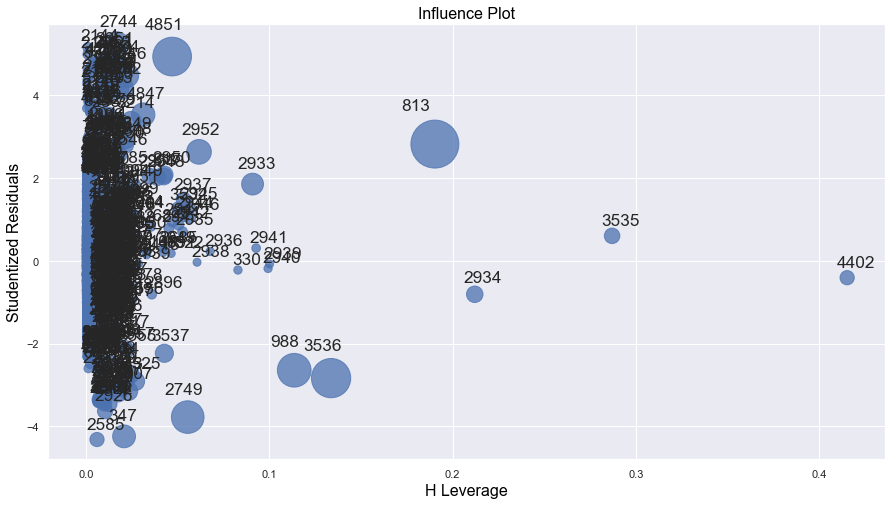
\includegraphics[keepaspectratio]{Lec5_Potential_issues_files/figure-pdf/cell-15-output-1.png}}

Let us identify the high leverage points in the data, as they may be
affecting the regression line if they are outliers as well, i.e., if
they are influential points. Note that there is no defined threshold for
a point to be classified as a high leverage point. Some statisticians
consider points having twice the average leverage as high leverage
points, some consider points having thrice the average leverage as high
leverage points, and so on.

\begin{Shaded}
\begin{Highlighting}[]
\NormalTok{out }\OperatorTok{=}\NormalTok{ model\_log.outlier\_test()}
\end{Highlighting}
\end{Shaded}

\begin{Shaded}
\begin{Highlighting}[]
\CommentTok{\#Average leverage of points}
\NormalTok{average\_leverage }\OperatorTok{=}\NormalTok{ (model\_log.df\_model}\OperatorTok{+}\DecValTok{1}\NormalTok{)}\OperatorTok{/}\NormalTok{model\_log.nobs}
\NormalTok{average\_leverage}
\end{Highlighting}
\end{Shaded}

\begin{verbatim}
0.0024193548387096775
\end{verbatim}

Let us consider points having four times the average leverage as high
leverage points.

\begin{Shaded}
\begin{Highlighting}[]
\CommentTok{\#We will remove all observations that have leverage higher than the threshold value.}
\NormalTok{high\_leverage\_threshold }\OperatorTok{=} \DecValTok{3}\OperatorTok{*}\NormalTok{average\_leverage}
\end{Highlighting}
\end{Shaded}

\begin{Shaded}
\begin{Highlighting}[]
\CommentTok{\#Number of high leverage points in the dataset}
\NormalTok{np.}\BuiltInTok{sum}\NormalTok{(leverage}\OperatorTok{\textgreater{}}\NormalTok{high\_leverage\_threshold)}
\end{Highlighting}
\end{Shaded}

\begin{verbatim}
269
\end{verbatim}

\subsection{Identifying extrapolation using
leverage}\label{identifying-extrapolation-using-leverage}

Leverage can be used to check if prediction on a particular point will
lead to extrapolation.

Below is the function that can be used to find the leverage at for a
particular observation \texttt{xnew}. Note that \texttt{xnew} has to be
a single-dimensional array, and \texttt{X} has to be the predictor
matrix (also called the design matrix).

\begin{Shaded}
\begin{Highlighting}[]
\KeywordTok{def}\NormalTok{ leverage\_compute(xnew, X):}
    \ControlFlowTok{return}\NormalTok{(xnew.reshape(}\OperatorTok{{-}}\DecValTok{1}\NormalTok{, }\DecValTok{1}\NormalTok{).T.dot(np.linalg.inv(X.T.dot(X))).dot(xnew.reshape(}\OperatorTok{{-}}\DecValTok{1}\NormalTok{, }\DecValTok{1}\NormalTok{))[}\DecValTok{0}\NormalTok{][}\DecValTok{0}\NormalTok{])}
\end{Highlighting}
\end{Shaded}

As expected, the function will return the same leverage as provided by
the \texttt{hat\_matrix\_diag} attribute of the objected returned by the
\texttt{get\_influence()} method of \texttt{model\_log} as shown below:

\begin{Shaded}
\begin{Highlighting}[]
\NormalTok{leverage[}\DecValTok{0}\NormalTok{]}
\end{Highlighting}
\end{Shaded}

\begin{verbatim}
0.0026426981240353694
\end{verbatim}

As the observation for prediction is required we need to create the
predictor matrix \texttt{X} to create all the observations with the
interactions specified in the model.

\begin{Shaded}
\begin{Highlighting}[]
\NormalTok{y, X }\OperatorTok{=}\NormalTok{ dmatrices(}\StringTok{\textquotesingle{}np.log(price)\textasciitilde{}(year+engineSize+mileage+mpg)**2+I(mileage**2)\textquotesingle{}}\NormalTok{, data }\OperatorTok{=}\NormalTok{ train)}
\end{Highlighting}
\end{Shaded}

\begin{Shaded}
\begin{Highlighting}[]
\NormalTok{leverage\_compute(X[}\DecValTok{0}\NormalTok{,:], X)}
\end{Highlighting}
\end{Shaded}

\begin{verbatim}
0.0026426973869101977
\end{verbatim}

If the leverage for a new observation is higher than the maximum
leverage among all the observations in the training dataset, then
prediction at the new observation will be extrapolation.

\section{Influential points}\label{influential-points}

Observations that are both high leverage points and outliers are
influential points that may affect the regression line. Let's remove
these influential points from the data and see if it improves the model
prediction accuracy on test data.

\begin{Shaded}
\begin{Highlighting}[]
\CommentTok{\#Dropping influential points from data}
\NormalTok{train\_filtered }\OperatorTok{=}\NormalTok{ train.drop(np.intersect1d(np.where(np.}\BuiltInTok{abs}\NormalTok{(out.student\_resid) }\OperatorTok{\textgreater{}}\NormalTok{ critical\_value)[}\DecValTok{0}\NormalTok{],}
\NormalTok{                                           (np.where(leverage}\OperatorTok{\textgreater{}}\NormalTok{high\_leverage\_threshold)[}\DecValTok{0}\NormalTok{])))}
\end{Highlighting}
\end{Shaded}

Note that as the Bonferroni's critical value is very conservative
estimate, we have rounded off the critical value to 4, instead of 4.42.

\begin{Shaded}
\begin{Highlighting}[]
\NormalTok{train\_filtered.shape}
\end{Highlighting}
\end{Shaded}

\begin{verbatim}
(4948, 11)
\end{verbatim}

\begin{Shaded}
\begin{Highlighting}[]
\CommentTok{\#Number of points removed as they were influential}
\NormalTok{train.shape[}\DecValTok{0}\NormalTok{]}\OperatorTok{{-}}\NormalTok{train\_filtered.shape[}\DecValTok{0}\NormalTok{]}
\end{Highlighting}
\end{Shaded}

\begin{verbatim}
12
\end{verbatim}

We removed 12 influential data points from the training data.

\begin{Shaded}
\begin{Highlighting}[]
\CommentTok{\#Model after removing the influential observations}
\NormalTok{ols\_object }\OperatorTok{=}\NormalTok{ smf.ols(formula }\OperatorTok{=} \StringTok{\textquotesingle{}np.log(price)\textasciitilde{}(year+engineSize+mileage+mpg)**2+I(mileage**2)\textquotesingle{}}\NormalTok{, data }\OperatorTok{=}\NormalTok{ train\_filtered)}
\NormalTok{model\_log }\OperatorTok{=}\NormalTok{ ols\_object.fit()}
\NormalTok{model\_log.summary()}
\end{Highlighting}
\end{Shaded}

\begin{center}
\begin{tabular}{lclc}
\toprule
\textbf{Dep. Variable:}     &  np.log(price)   & \textbf{  R-squared:         } &     0.815   \\
\textbf{Model:}             &       OLS        & \textbf{  Adj. R-squared:    } &     0.814   \\
\textbf{Method:}            &  Least Squares   & \textbf{  F-statistic:       } &     1971.   \\
\textbf{Date:}              & Sun, 10 Mar 2024 & \textbf{  Prob (F-statistic):} &     0.00    \\
\textbf{Time:}              &     16:54:08     & \textbf{  Log-Likelihood:    } &   -1027.9   \\
\textbf{No. Observations:}  &        4948      & \textbf{  AIC:               } &     2080.   \\
\textbf{Df Residuals:}      &        4936      & \textbf{  BIC:               } &     2158.   \\
\textbf{Df Model:}          &          11      & \textbf{                     } &             \\
\textbf{Covariance Type:}   &    nonrobust     & \textbf{                     } &             \\
\bottomrule
\end{tabular}
\begin{tabular}{lcccccc}
                            & \textbf{coef} & \textbf{std err} & \textbf{t} & \textbf{P$> |$t$|$} & \textbf{[0.025} & \textbf{0.975]}  \\
\midrule
\textbf{Intercept}          &    -256.2339  &       25.421     &   -10.080  &         0.000        &     -306.070    &     -206.398     \\
\textbf{year}               &       0.1317  &        0.013     &    10.462  &         0.000        &        0.107    &        0.156     \\
\textbf{engineSize}         &      18.4650  &        5.663     &     3.261  &         0.001        &        7.364    &       29.566     \\
\textbf{mileage}            &       0.0006  &        0.000     &     4.288  &         0.000        &        0.000    &        0.001     \\
\textbf{mpg}                &      -1.1810  &        0.338     &    -3.489  &         0.000        &       -1.845    &       -0.517     \\
\textbf{year:engineSize}    &      -0.0090  &        0.003     &    -3.208  &         0.001        &       -0.015    &       -0.004     \\
\textbf{year:mileage}       &   -2.933e-07  &      6.7e-08     &    -4.374  &         0.000        &    -4.25e-07    &    -1.62e-07     \\
\textbf{year:mpg}           &       0.0006  &        0.000     &     3.458  &         0.001        &        0.000    &        0.001     \\
\textbf{engineSize:mileage} &   -4.316e-07  &        4e-07     &    -1.080  &         0.280        &    -1.21e-06    &     3.52e-07     \\
\textbf{engineSize:mpg}     &       0.0048  &        0.000     &    11.537  &         0.000        &        0.004    &        0.006     \\
\textbf{mileage:mpg}        &    7.254e-08  &     1.75e-08     &     4.140  &         0.000        &     3.82e-08    &     1.07e-07     \\
\textbf{I(mileage ** 2)}    &    1.668e-11  &     5.53e-12     &     3.017  &         0.003        &     5.84e-12    &     2.75e-11     \\
\bottomrule
\end{tabular}
\begin{tabular}{lclc}
\textbf{Omnibus:}       & 718.619 & \textbf{  Durbin-Watson:     } &    0.521  \\
\textbf{Prob(Omnibus):} &   0.000 & \textbf{  Jarque-Bera (JB):  } & 2512.509  \\
\textbf{Skew:}          &   0.714 & \textbf{  Prob(JB):          } &     0.00  \\
\textbf{Kurtosis:}      &   6.185 & \textbf{  Cond. No.          } & 1.75e+13  \\
\bottomrule
\end{tabular}
%\caption{OLS Regression Results}
\end{center}

Notes: \newline
 [1] Standard Errors assume that the covariance matrix of the errors is correctly specified. \newline
 [2] The condition number is large, 1.75e+13. This might indicate that there are \newline
 strong multicollinearity or other numerical problems.

Let us compare the square root of 5-fold cross-validated mean squared
error of the model with and without the influential points.

\begin{Shaded}
\begin{Highlighting}[]
\NormalTok{y, X }\OperatorTok{=}\NormalTok{ dmatrices(}\StringTok{\textquotesingle{}np.log(price)\textasciitilde{}(year+engineSize+mileage+mpg)**2+I(mileage**2)\textquotesingle{}}\NormalTok{, data }\OperatorTok{=}\NormalTok{ train)}
\NormalTok{np.sqrt(mean\_squared\_error(np.exp(cross\_val\_predict(LinearRegression(), X, y)), np.exp(y)))}
\end{Highlighting}
\end{Shaded}

\begin{verbatim}
9811.74078331643
\end{verbatim}

\begin{Shaded}
\begin{Highlighting}[]
\NormalTok{y, X }\OperatorTok{=}\NormalTok{ dmatrices(}\StringTok{\textquotesingle{}np.log(price)\textasciitilde{}(year+engineSize+mileage+mpg)**2+I(mileage**2)\textquotesingle{}}\NormalTok{, data }\OperatorTok{=}\NormalTok{ train\_filtered)}
\NormalTok{np.sqrt(mean\_squared\_error(np.exp(cross\_val\_predict(LinearRegression(), X, y)), np.exp(y)))}
\end{Highlighting}
\end{Shaded}

\begin{verbatim}
9800.202063309154
\end{verbatim}

\textbf{Why can't we use \texttt{cross\_val\_score()} instead of
\texttt{cross\_val\_predict()} here?}

There seems to be a slight improvement in prediction error after
removing influential points. Note that none of the points had ``very
high leverage'', and thus the change is not substantial.

Note that we obtain a higher R-squared value of 81.5\% as compared to
80\% with the complete data. Removing the influential points helped
obtain a slightly better model fit. However, that may also happen just
by reducing observations.

\begin{Shaded}
\begin{Highlighting}[]
\CommentTok{\#Computing RMSE on test data}
\NormalTok{pred\_price\_log }\OperatorTok{=}\NormalTok{ model\_log.predict(testf)}
\NormalTok{np.sqrt(((testp.price }\OperatorTok{{-}}\NormalTok{ np.exp(pred\_price\_log))}\OperatorTok{**}\DecValTok{2}\NormalTok{).mean())}
\end{Highlighting}
\end{Shaded}

\begin{verbatim}
8922.977452912108
\end{verbatim}

The RMSE on test data has also reduced. This shows that some of the
influential points were impacting the regression line. With those points
removed, the model better captures the general trend in the data.

\subsection{Influence on single fitted value
(DFFITS)}\label{influence-on-single-fitted-value-dffits}

\begin{itemize}
\tightlist
\item
  A useful measure of the influence that the \(i^{th}\) observation has
  on the fitted value \(\hat{Y}_i\) is:
\end{itemize}

\begin{equation}
(DFFITS)_i = \frac{\hat{Y}_i-\hat{Y}_{i(i)}}{\sqrt{MSE_{i}h_i}}
\end{equation}

\begin{itemize}
\item
  Note that the denominator in the above fraction is the estimated
  standard deviation of \(\hat{Y}_i\), but uses the error mean square
  when the \(i^{th}\) observation is omitted.
\item
  \(DFFITS\) for the \(i^{th}\) observation represents the number of
  estimated standard deviations of \(\hat{Y}_i\) that the fitted value
  \(\hat{Y}_i\) increases or decreases with the inclusion of the
  \(i^{th}\) observation in fitting the regression model.
\item
  It can be shown that:
\end{itemize}

\begin{equation}
(DFFITS)_i = t_i\sqrt{\frac{h_i}{1-h_i}}
\end{equation}

where \(t_i\) is the studentized deleted residual for the \(i^{th}\)
observation.

\begin{itemize}
\item
  We can see that if an observation has high leverage and is an outlier,
  it is likely to be influential
\item
  For large datasets, an observation is considered influential if the
  magnitude of \(DFFITS\) for it exceeds \(2\sqrt{\frac{p}{n}}\)
\end{itemize}

\begin{Shaded}
\begin{Highlighting}[]
\NormalTok{sns.}\BuiltInTok{set}\NormalTok{(font\_scale }\OperatorTok{=}\FloatTok{1.5}\NormalTok{)}
\NormalTok{sns.lineplot(x }\OperatorTok{=} \BuiltInTok{range}\NormalTok{(train.shape[}\DecValTok{0}\NormalTok{]), y }\OperatorTok{=}\NormalTok{ influence.dffits[}\DecValTok{0}\NormalTok{])}
\NormalTok{plt.xlabel(}\StringTok{\textquotesingle{}Observation index\textquotesingle{}}\NormalTok{)}
\NormalTok{plt.ylabel(}\StringTok{\textquotesingle{}DFFITS (model)\textquotesingle{}}\NormalTok{)}\OperatorTok{;}
\end{Highlighting}
\end{Shaded}

\pandocbounded{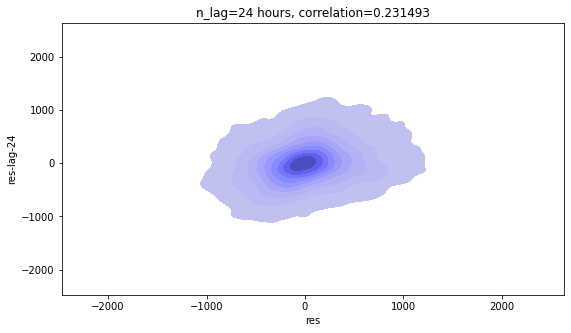
\includegraphics[keepaspectratio]{Lec5_Potential_issues_files/figure-pdf/cell-31-output-1.png}}

\textbf{Let us analyze the point with the highest \(DFFITS\)}.

\begin{Shaded}
\begin{Highlighting}[]
\NormalTok{np.where(influence.dffits[}\DecValTok{0}\NormalTok{]}\OperatorTok{\textgreater{}}\DecValTok{1}\NormalTok{)}
\end{Highlighting}
\end{Shaded}

\begin{verbatim}
(array([ 813, 4851], dtype=int64),)
\end{verbatim}

\begin{Shaded}
\begin{Highlighting}[]
\NormalTok{train.loc[}\DecValTok{813}\NormalTok{,:]}
\end{Highlighting}
\end{Shaded}

\begin{verbatim}
carID                12454
brand                   vw
model            Caravelle
year                  2012
transmission     Semi-Auto
mileage             212000
fuelType            Diesel
tax                    325
mpg                34.4424
engineSize             2.0
price                11995
Name: 813, dtype: object
\end{verbatim}

\begin{Shaded}
\begin{Highlighting}[]
\NormalTok{train.loc[train.model }\OperatorTok{==} \StringTok{\textquotesingle{} Caravelle\textquotesingle{}}\NormalTok{,}\StringTok{\textquotesingle{}mileage\textquotesingle{}}\NormalTok{].describe()}
\end{Highlighting}
\end{Shaded}

\begin{verbatim}
count        65.000000
mean      25638.692308
std       42954.135726
min          10.000000
25%        3252.000000
50%        6900.000000
75%       30414.000000
max      212000.000000
Name: mileage, dtype: float64
\end{verbatim}

\begin{Shaded}
\begin{Highlighting}[]
\CommentTok{\# Prediction with model developed based on all points}
\NormalTok{ols\_object }\OperatorTok{=}\NormalTok{ smf.ols(formula }\OperatorTok{=} \StringTok{\textquotesingle{}np.log(price)\textasciitilde{}(year+engineSize+mileage+mpg)**2+I(mileage**2)\textquotesingle{}}\NormalTok{, }
\NormalTok{                     data }\OperatorTok{=}\NormalTok{ train)}
\NormalTok{model\_log }\OperatorTok{=}\NormalTok{ ols\_object.fit()}\OperatorTok{;}
\NormalTok{np.exp(model\_log.predict(train.loc[[}\DecValTok{813}\NormalTok{],:]))}
\end{Highlighting}
\end{Shaded}

\begin{verbatim}
813    5502.647323
dtype: float64
\end{verbatim}

\begin{Shaded}
\begin{Highlighting}[]
\CommentTok{\# Prediction with model developed based on all points except the 813th point}
\NormalTok{ols\_object }\OperatorTok{=}\NormalTok{ smf.ols(formula }\OperatorTok{=} \StringTok{\textquotesingle{}np.log(price)\textasciitilde{}(year+engineSize+mileage+mpg)**2+I(mileage**2)\textquotesingle{}}\NormalTok{, }
\NormalTok{                     data }\OperatorTok{=}\NormalTok{ train.drop(index }\OperatorTok{=} \DecValTok{813}\NormalTok{))}
\NormalTok{model\_log }\OperatorTok{=}\NormalTok{ ols\_object.fit()}\OperatorTok{;}
\NormalTok{np.exp(model\_log.predict(train.loc[[}\DecValTok{813}\NormalTok{],:]))}
\end{Highlighting}
\end{Shaded}

\begin{verbatim}
813    4581.374593
dtype: float64
\end{verbatim}

Let us see the leverage and studentized residual for this observation.

\begin{Shaded}
\begin{Highlighting}[]
\CommentTok{\# Leverage}
\NormalTok{leverage[}\DecValTok{813}\NormalTok{]}
\end{Highlighting}
\end{Shaded}

\begin{verbatim}
0.19038697461006687
\end{verbatim}

\begin{Shaded}
\begin{Highlighting}[]
\CommentTok{\# Studentized residual}
\NormalTok{out.student\_resid[}\DecValTok{813}\NormalTok{]}
\end{Highlighting}
\end{Shaded}

\begin{verbatim}
2.823478041409651
\end{verbatim}

\textbf{Do you notice what may be contributing to the high influence of
this point?}

\subsection{Influence on all fitted values (Cook's
distance)}\label{influence-on-all-fitted-values-cooks-distance}

In contrast to \(DFFITS\), which considers the influence of the
\(i^{th}\) observation on the fitted value \(\hat{Y}_i\), Cook's
distance considers the influence of the \(i^{th}\) observation on all
\(n\) the fitted values:

\begin{equation}
D_i = \frac{\sum_{j=1}^{n} (\hat{Y}_j - \hat{Y}_{j(i)})^2}{pMSE}
\end{equation}

It can be shown that:

\begin{equation}
D_i = \frac{e_i^2}{pMSE}\bigg[\frac{h_i}{(1-h_i)^2}\bigg]
\end{equation}

The larger \(h_i\) or \(e_i\), the larger is \(D_i\). \(D_i\) can be
related to the \(F(p, n- p)\) distribution. If the percentile value is
50\% or more, the observation is considered as highly influential.

Cook's distance is considered high if it is greater than 0.5 and extreme
if it is greater than 1.

\begin{Shaded}
\begin{Highlighting}[]
\NormalTok{sns.}\BuiltInTok{set}\NormalTok{(font\_scale }\OperatorTok{=}\FloatTok{1.5}\NormalTok{)}
\NormalTok{sns.lineplot(x }\OperatorTok{=} \BuiltInTok{range}\NormalTok{(train.shape[}\DecValTok{0}\NormalTok{]), y }\OperatorTok{=}\NormalTok{ influence.cooks\_distance[}\DecValTok{0}\NormalTok{])}
\NormalTok{plt.xlabel(}\StringTok{\textquotesingle{}Observation index\textquotesingle{}}\NormalTok{)}
\NormalTok{plt.ylabel(}\StringTok{"Cook\textquotesingle{}s Distance (model)"}\NormalTok{)}\OperatorTok{;}
\end{Highlighting}
\end{Shaded}

\pandocbounded{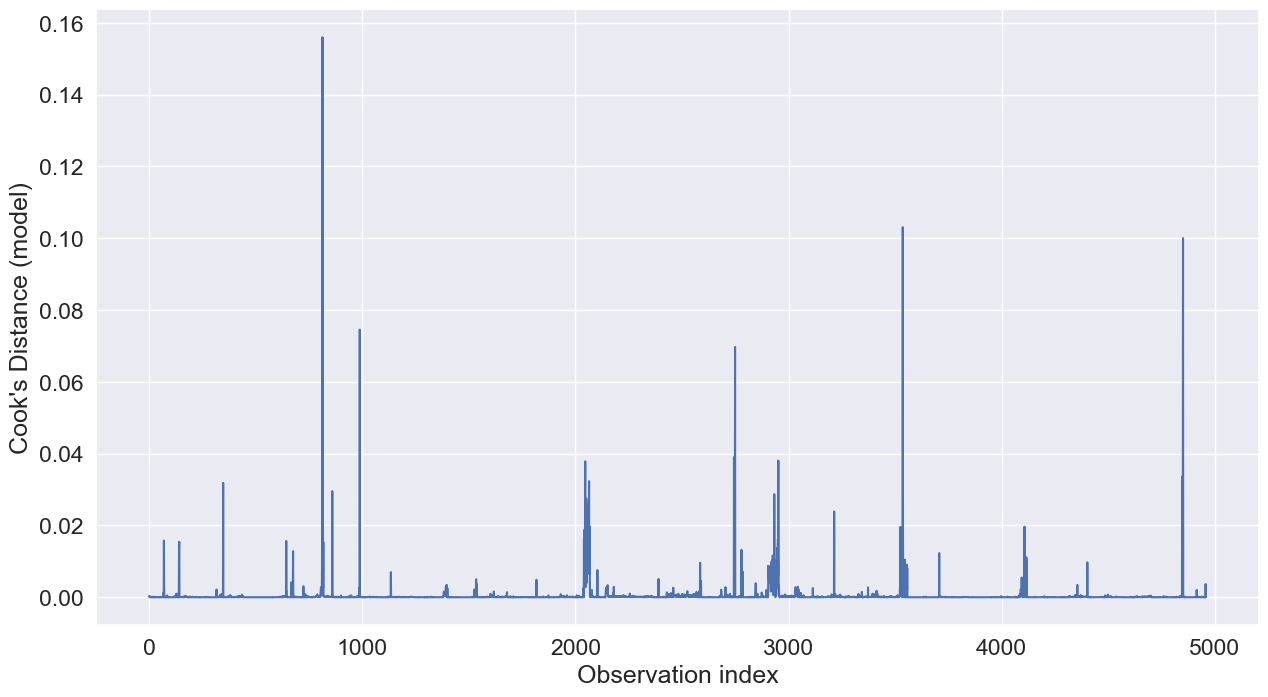
\includegraphics[keepaspectratio]{Lec5_Potential_issues_files/figure-pdf/cell-39-output-1.png}}

\begin{Shaded}
\begin{Highlighting}[]
\CommentTok{\# Point with the highest Cook\textquotesingle{}s distance}
\NormalTok{np.where(influence.cooks\_distance[}\DecValTok{0}\NormalTok{]}\OperatorTok{\textgreater{}}\FloatTok{0.15}\NormalTok{)}
\end{Highlighting}
\end{Shaded}

\begin{verbatim}
(array([813], dtype=int64),)
\end{verbatim}

The critical Cook's distance value for a point to be highly influential
in this dataset is:

\begin{Shaded}
\begin{Highlighting}[]
\NormalTok{stats.f.ppf(}\FloatTok{0.5}\NormalTok{, }\DecValTok{11}\NormalTok{, }\DecValTok{4949}\NormalTok{)}
\end{Highlighting}
\end{Shaded}

\begin{verbatim}
0.9402181103263811
\end{verbatim}

Thus, we don't have any highly influential points in the dataset.

\subsection{Influence on regression coefficients
(DFBETAS)}\label{influence-on-regression-coefficients-dfbetas}

\begin{itemize}
\item
  \(DFBETAS\) measures the influence of the \(i^{th}\) observation on
  the regression coefficient.
\item
  \(DFBETAS\) of the \(i^{th}\) observation on the \(k^{th}\) regression
  coefficient is:
\end{itemize}

\begin{equation}
(DFBETAS)_{k(i)} = \frac{\hat{\beta}_k-\hat{\beta}_{k(i)}}{\sqrt{MSE_ic_{k}}}
\end{equation}

where \(c_k\) is the \(k^{th}\) diagonal element of \((X^TX)^{-1}\).

For large datasets, an observation is considered influential if
\(DFBETAS\) exceeds \(\frac{2}{\sqrt{n}}\).

Below is the plot of \(DFBETAS\) for the \texttt{year} predictor against
the observation index.

\begin{Shaded}
\begin{Highlighting}[]
\NormalTok{sns.}\BuiltInTok{set}\NormalTok{(font\_scale }\OperatorTok{=}\FloatTok{1.5}\NormalTok{)}
\NormalTok{sns.lineplot(x }\OperatorTok{=} \BuiltInTok{range}\NormalTok{(train.shape[}\DecValTok{0}\NormalTok{]), y }\OperatorTok{=}\NormalTok{ influence.dfbetas[:,}\DecValTok{1}\NormalTok{])}
\NormalTok{plt.xlabel(}\StringTok{\textquotesingle{}Observation index\textquotesingle{}}\NormalTok{)}
\NormalTok{plt.ylabel(}\StringTok{"DFBETAS (year)"}\NormalTok{)}\OperatorTok{;}
\end{Highlighting}
\end{Shaded}

\pandocbounded{\includegraphics[keepaspectratio]{Lec5_Potential_issues_files/figure-pdf/cell-42-output-1.png}}

Let us analyze the point with the highest magnitude of \(DFBETAS\).

\begin{Shaded}
\begin{Highlighting}[]
\NormalTok{np.where(influence.dfbetas[:,}\DecValTok{1}\NormalTok{]}\OperatorTok{\textless{}{-}}\FloatTok{0.8}\NormalTok{)}
\end{Highlighting}
\end{Shaded}

\begin{verbatim}
(array([4851], dtype=int64),)
\end{verbatim}

\begin{Shaded}
\begin{Highlighting}[]
\NormalTok{train.year.describe()}
\end{Highlighting}
\end{Shaded}

\begin{verbatim}
count    4960.000000
mean     2016.737903
std         2.884035
min      1997.000000
25%      2016.000000
50%      2017.000000
75%      2019.000000
max      2020.000000
Name: year, dtype: float64
\end{verbatim}

\begin{Shaded}
\begin{Highlighting}[]
\NormalTok{train.loc[train.year}\OperatorTok{\textless{}=}\DecValTok{2002}\NormalTok{,:]}
\end{Highlighting}
\end{Shaded}

\begin{longtable}[]{@{}llllllllllll@{}}
\toprule\noalign{}
& carID & brand & model & year & transmission & mileage & fuelType & tax
& mpg & engineSize & price \\
\midrule\noalign{}
\endhead
\bottomrule\noalign{}
\endlastfoot
330 & 13200 & audi & A8 & 1997 & Automatic & 122000 & Petrol & 265 &
19.3511 & 4.2 & 4650 \\
732 & 13988 & vw & Beetle & 2001 & Manual & 47729 & Petrol & 330 &
32.5910 & 2.0 & 2490 \\
3157 & 18794 & ford & Puma & 2002 & Manual & 108000 & Petrol & 230 &
38.5757 & 1.7 & 2195 \\
3525 & 19395 & merc & S Class & 2001 & Automatic & 108800 & Diesel & 325
& 31.5473 & 3.2 & 1695 \\
3532 & 17531 & merc & S Class & 1999 & Automatic & 34000 & Petrol & 145
& 24.8735 & 3.2 & 5995 \\
3533 & 18761 & merc & S Class & 2001 & Automatic & 66000 & Petrol & 570
& 24.7744 & 3.2 & 4495 \\
3535 & 18813 & merc & S Class & 1998 & Automatic & 43534 & Petrol & 265
& 23.2962 & 6.0 & 19990 \\
3536 & 17891 & merc & S Class & 2002 & Automatic & 24000 & Petrol & 570
& 20.7968 & 5.0 & 6995 \\
3707 & 18746 & hyundi & Santa Fe & 2002 & Manual & 94000 & Petrol & 325
& 30.2671 & 2.4 & 1200 \\
4091 & 12995 & merc & SLK & 1998 & Automatic & 113557 & Petrol & 265 &
31.8368 & 2.3 & 1990 \\
4094 & 19585 & merc & SLK & 2001 & Automatic & 69234 & Petrol & 325 &
30.8839 & 2.0 & 3990 \\
4096 & 14265 & merc & SLK & 2001 & Automatic & 48172 & Petrol & 325 &
29.7058 & 2.3 & 3990 \\
4097 & 15821 & merc & SLK & 2002 & Automatic & 61400 & Petrol & 325 &
29.6568 & 2.3 & 3990 \\
4098 & 13021 & merc & SLK & 2001 & Automatic & 91000 & Petrol & 325 &
30.3248 & 2.3 & 3950 \\
4099 & 12660 & merc & SLK & 2001 & Automatic & 42087 & Petrol & 325 &
29.9404 & 2.3 & 4490 \\
4101 & 17521 & merc & SLK & 2002 & Automatic & 75034 & Petrol & 325 &
30.1380 & 2.3 & 4990 \\
4107 & 13977 & merc & SLK & 2000 & Automatic & 87000 & Petrol & 265 &
27.2998 & 3.2 & 1490 \\
4108 & 18679 & merc & SLK & 2000 & Automatic & 113237 & Petrol & 270 &
26.8765 & 3.2 & 3990 \\
4109 & 14598 & merc & SLK & 2001 & Automatic & 64476 & Petrol & 325 &
27.4628 & 3.2 & 4990 \\
4847 & 17268 & bmw & Z3 & 1997 & Manual & 49000 & Petrol & 270 & 34.9548
& 1.9 & 3950 \\
4848 & 12137 & bmw & Z3 & 1999 & Manual & 58000 & Petrol & 270 & 35.3077
& 1.9 & 3950 \\
4849 & 13288 & bmw & Z3 & 1999 & Manual & 74282 & Petrol & 245 & 35.4143
& 1.9 & 3995 \\
4850 & 19172 & bmw & Z3 & 2001 & Manual & 60000 & Petrol & 325 & 30.7305
& 2.2 & 5950 \\
4851 & 16577 & bmw & Z3 & 2002 & Automatic & 16500 & Petrol & 325 &
29.7614 & 2.2 & 14995 \\
\end{longtable}

Let us see the leverage and studentized residual for this observation.

\begin{Shaded}
\begin{Highlighting}[]
\CommentTok{\# Leverage}
\NormalTok{leverage[}\DecValTok{4851}\NormalTok{]}
\end{Highlighting}
\end{Shaded}

\begin{verbatim}
0.047120455781282225
\end{verbatim}

\begin{Shaded}
\begin{Highlighting}[]
\CommentTok{\# Studentized residual}
\NormalTok{out.student\_resid[}\DecValTok{4851}\NormalTok{]}
\end{Highlighting}
\end{Shaded}

\begin{verbatim}
4.938606329343604
\end{verbatim}

\textbf{Do you see what makes this point influential?}

\section{Collinearity}\label{collinearity}

Collinearity refers to the situation when two or more predictor
variables have a high linear association. Linear association between a
pair of variables can be measured by the correlation coefficient. Thus
the correlation matrix can indicate some potential collinearity
problems.

\subsection{Why and how is collinearity a
problem}\label{why-and-how-is-collinearity-a-problem}

\emph{(Source: page 100-101 of book)}

The presence of collinearity can pose problems in the regression
context, since it can be difficult to separate out the individual
effects of collinear variables on the response.

Since collinearity reduces the accuracy of the estimates of the
regression coefficients, it causes the standard error for
\(\hat \beta_j\) to grow. Recall that the t-statistic for each predictor
is calculated by dividing \(\hat \beta_j\) by its standard error.
Consequently, collinearity results in a decline in the \(t\)-statistic.
As a result, \textbf{in the presence of collinearity, we may fail to
reject \(H_0: \beta_j = 0\). This means that the power of the hypothesis
test---the probability of correctly detecting a non-zero
coefficient---is reduced by collinearity.}

\subsection{How to measure
collinearity/multicollinearity}\label{how-to-measure-collinearitymulticollinearity}

\emph{(Source: page 102 of book)}

Unfortunately, not all collinearity problems can be detected by
inspection of the correlation matrix: it is possible for collinearity to
exist between three or more variables even if no pair of variables has a
particularly high correlation. We call this situation multicollinearity.
Instead of inspecting the correlation matrix, a better way to assess
multicollinearity is to compute the variance inflation factor (VIF). The
VIF is variance inflation factor the ratio of the variance of
\(\hat \beta_j\) when fitting the full model divided by the variance of
\(\hat \beta_j\) if fit on its own. The smallest possible value for VIF
is 1, which indicates the complete absence of collinearity. Typically in
practice there is a small amount of collinearity among the predictors.
As a rule of thumb, a \textbf{VIF value that exceeds 5 or 10 indicates a
problematic amount of collinearity.}

The estimated variance of the coefficient \(\beta_j\), of the \(j^{th}\)
predictor \(X_j\), can be expressed as:

\[\hat{var}(\hat{\beta_j}) = \frac{(\hat{\sigma})^2}{(n-1)\hat{var}({X_j})}.\frac{1}{1-R^2_{X_j|X_{-j}}},\]

where \(R^2_{X_j|X_{-j}}\) is the \(R\)-squared for the regression of
\(X_j\) on the other covariates (a regression that does not involve the
response variable \(Y\)).

In case of simple linear regression, the variance expression in the
equation above does not contain the term
\(\frac{1}{1-R^2_{X_j|X_{-j}}}\), as there is only one predictor.
However, in case of multiple linear regression, the variance of the
estimate of the \(j^{th}\) coefficient (\(\hat{\beta_j}\)) gets inflated
by a factor of \(\frac{1}{1-R^2_{X_j|X_{-j}}}\) \emph{(Note that in the
complete absence of collinearity, \(R^2_{X_j|X_{-j}}=0\), and the value
of this factor will be 1).}

Thus, the Variance inflation factor, or the VIF for the estimated
coefficient of the \(j^{th}\) predictor \(X_j\) is:

\begin{equation}
VIF(\hat \beta_j) = \frac{1}{1-R^2_{X_j|X_{-j}}}
\end{equation}

\begin{Shaded}
\begin{Highlighting}[]
\CommentTok{\#Correlation matrix}
\NormalTok{train.corr()}
\end{Highlighting}
\end{Shaded}

\begin{longtable}[]{@{}llllllll@{}}
\toprule\noalign{}
& carID & year & mileage & tax & mpg & engineSize & price \\
\midrule\noalign{}
\endhead
\bottomrule\noalign{}
\endlastfoot
carID & 1.000000 & 0.006251 & -0.001320 & 0.023806 & -0.010774 &
0.011365 & 0.012129 \\
year & 0.006251 & 1.000000 & -0.768058 & -0.205902 & -0.057093 &
0.014623 & 0.501296 \\
mileage & -0.001320 & -0.768058 & 1.000000 & 0.133744 & 0.125376 &
-0.006459 & -0.478705 \\
tax & 0.023806 & -0.205902 & 0.133744 & 1.000000 & -0.488002 & 0.465282
& 0.144652 \\
mpg & -0.010774 & -0.057093 & 0.125376 & -0.488002 & 1.000000 &
-0.419417 & -0.369919 \\
engineSize & 0.011365 & 0.014623 & -0.006459 & 0.465282 & -0.419417 &
1.000000 & 0.624899 \\
price & 0.012129 & 0.501296 & -0.478705 & 0.144652 & -0.369919 &
0.624899 & 1.000000 \\
\end{longtable}

Let us compute the Variance Inflation Factor (VIF) for the four
predictors.

\begin{Shaded}
\begin{Highlighting}[]
\NormalTok{X }\OperatorTok{=}\NormalTok{ train[[}\StringTok{\textquotesingle{}mpg\textquotesingle{}}\NormalTok{,}\StringTok{\textquotesingle{}year\textquotesingle{}}\NormalTok{,}\StringTok{\textquotesingle{}mileage\textquotesingle{}}\NormalTok{,}\StringTok{\textquotesingle{}engineSize\textquotesingle{}}\NormalTok{]]}
\end{Highlighting}
\end{Shaded}

\begin{Shaded}
\begin{Highlighting}[]
\NormalTok{X.columns[}\DecValTok{1}\NormalTok{:]}
\end{Highlighting}
\end{Shaded}

\begin{verbatim}
Index(['year', 'mileage', 'engineSize'], dtype='object')
\end{verbatim}

\begin{Shaded}
\begin{Highlighting}[]
\ImportTok{from}\NormalTok{ statsmodels.stats.outliers\_influence }\ImportTok{import}\NormalTok{ variance\_inflation\_factor}
\ImportTok{from}\NormalTok{ statsmodels.tools.tools }\ImportTok{import}\NormalTok{ add\_constant}
\NormalTok{X }\OperatorTok{=}\NormalTok{ add\_constant(X)}
\NormalTok{vif\_data }\OperatorTok{=}\NormalTok{ pd.DataFrame()}
\NormalTok{vif\_data[}\StringTok{"feature"}\NormalTok{] }\OperatorTok{=}\NormalTok{ X.columns}

\ControlFlowTok{for}\NormalTok{ i }\KeywordTok{in} \BuiltInTok{range}\NormalTok{(}\BuiltInTok{len}\NormalTok{(X.columns)):}
\NormalTok{    vif\_data.loc[i,}\StringTok{\textquotesingle{}VIF\textquotesingle{}}\NormalTok{] }\OperatorTok{=}\NormalTok{ variance\_inflation\_factor(X.values, i)}

\BuiltInTok{print}\NormalTok{(vif\_data)}
\end{Highlighting}
\end{Shaded}

\begin{verbatim}
      feature           VIF
0       const  1.201579e+06
1         mpg  1.243040e+00
2        year  2.452891e+00
3     mileage  2.490210e+00
4  engineSize  1.219170e+00
\end{verbatim}

As all the values of VIF are close to one, we do not have the problem of
multicollinearity in the model. Note that the VIF of \texttt{year} and
\texttt{mileage} is relatively high as they are the most correlated.

\textbf{Q1:} Why is the VIF of the constant so high?

\textbf{Q2:} Why do we need to include the constant while finding the
VIF?

\subsection{Manual computation of VIF}\label{manual-computation-of-vif}

\begin{Shaded}
\begin{Highlighting}[]
\CommentTok{\#Manually computing the VIF for year}
\NormalTok{ols\_object }\OperatorTok{=}\NormalTok{ smf.ols(formula }\OperatorTok{=} \StringTok{\textquotesingle{}price\textasciitilde{}mpg\textquotesingle{}}\NormalTok{, data }\OperatorTok{=}\NormalTok{ train)}
\NormalTok{model\_log }\OperatorTok{=}\NormalTok{ ols\_object.fit()}
\NormalTok{model\_log.summary()}
\end{Highlighting}
\end{Shaded}

\begin{center}
\begin{tabular}{lclc}
\toprule
\textbf{Dep. Variable:}    &      price       & \textbf{  R-squared:         } &     0.137   \\
\textbf{Model:}            &       OLS        & \textbf{  Adj. R-squared:    } &     0.137   \\
\textbf{Method:}           &  Least Squares   & \textbf{  F-statistic:       } &     786.0   \\
\textbf{Date:}             & Wed, 06 Mar 2024 & \textbf{  Prob (F-statistic):} & 1.14e-160   \\
\textbf{Time:}             &     17:04:39     & \textbf{  Log-Likelihood:    } &   -54812.   \\
\textbf{No. Observations:} &        4960      & \textbf{  AIC:               } & 1.096e+05   \\
\textbf{Df Residuals:}     &        4958      & \textbf{  BIC:               } & 1.096e+05   \\
\textbf{Df Model:}         &           1      & \textbf{                     } &             \\
\textbf{Covariance Type:}  &    nonrobust     & \textbf{                     } &             \\
\bottomrule
\end{tabular}
\begin{tabular}{lcccccc}
                   & \textbf{coef} & \textbf{std err} & \textbf{t} & \textbf{P$> |$t$|$} & \textbf{[0.025} & \textbf{0.975]}  \\
\midrule
\textbf{Intercept} &    4.144e+04  &      676.445     &    61.258  &         0.000        &     4.01e+04    &     4.28e+04     \\
\textbf{mpg}       &    -374.2975  &       13.351     &   -28.036  &         0.000        &     -400.471    &     -348.124     \\
\bottomrule
\end{tabular}
\begin{tabular}{lclc}
\textbf{Omnibus:}       & 2132.208 & \textbf{  Durbin-Watson:     } &     0.320  \\
\textbf{Prob(Omnibus):} &   0.000  & \textbf{  Jarque-Bera (JB):  } & 13751.995  \\
\textbf{Skew:}          &   1.942  & \textbf{  Prob(JB):          } &      0.00  \\
\textbf{Kurtosis:}      &  10.174  & \textbf{  Cond. No.          } &      158.  \\
\bottomrule
\end{tabular}
%\caption{OLS Regression Results}
\end{center}

Notes: \newline
 [1] Standard Errors assume that the covariance matrix of the errors is correctly specified.

\begin{Shaded}
\begin{Highlighting}[]
\NormalTok{(}\FloatTok{13.351}\OperatorTok{/}\FloatTok{9.338}\NormalTok{)}\OperatorTok{**}\DecValTok{2}
\end{Highlighting}
\end{Shaded}

\begin{verbatim}
2.044183378279958
\end{verbatim}

\begin{Shaded}
\begin{Highlighting}[]
\CommentTok{\#Manually computing the VIF for year}
\NormalTok{ols\_object }\OperatorTok{=}\NormalTok{ smf.ols(formula }\OperatorTok{=} \StringTok{\textquotesingle{}price\textasciitilde{}year+mpg+engineSize+mileage\textquotesingle{}}\NormalTok{, data }\OperatorTok{=}\NormalTok{ train)}
\NormalTok{model\_log }\OperatorTok{=}\NormalTok{ ols\_object.fit()}
\NormalTok{model\_log.summary()}
\end{Highlighting}
\end{Shaded}

\begin{center}
\begin{tabular}{lclc}
\toprule
\textbf{Dep. Variable:}    &      price       & \textbf{  R-squared:         } &     0.660   \\
\textbf{Model:}            &       OLS        & \textbf{  Adj. R-squared:    } &     0.660   \\
\textbf{Method:}           &  Least Squares   & \textbf{  F-statistic:       } &     2410.   \\
\textbf{Date:}             & Wed, 06 Mar 2024 & \textbf{  Prob (F-statistic):} &     0.00    \\
\textbf{Time:}             &     17:01:18     & \textbf{  Log-Likelihood:    } &   -52497.   \\
\textbf{No. Observations:} &        4960      & \textbf{  AIC:               } & 1.050e+05   \\
\textbf{Df Residuals:}     &        4955      & \textbf{  BIC:               } & 1.050e+05   \\
\textbf{Df Model:}         &           4      & \textbf{                     } &             \\
\textbf{Covariance Type:}  &    nonrobust     & \textbf{                     } &             \\
\bottomrule
\end{tabular}
\begin{tabular}{lcccccc}
                    & \textbf{coef} & \textbf{std err} & \textbf{t} & \textbf{P$> |$t$|$} & \textbf{[0.025} & \textbf{0.975]}  \\
\midrule
\textbf{Intercept}  &   -3.661e+06  &     1.49e+05     &   -24.593  &         0.000        &    -3.95e+06    &    -3.37e+06     \\
\textbf{year}       &    1817.7366  &       73.751     &    24.647  &         0.000        &     1673.151    &     1962.322     \\
\textbf{mpg}        &     -79.3126  &        9.338     &    -8.493  &         0.000        &      -97.620    &      -61.006     \\
\textbf{engineSize} &    1.218e+04  &      189.969     &    64.107  &         0.000        &     1.18e+04    &     1.26e+04     \\
\textbf{mileage}    &      -0.1474  &        0.009     &   -16.817  &         0.000        &       -0.165    &       -0.130     \\
\bottomrule
\end{tabular}
\begin{tabular}{lclc}
\textbf{Omnibus:}       & 2450.973 & \textbf{  Durbin-Watson:     } &     0.541  \\
\textbf{Prob(Omnibus):} &   0.000  & \textbf{  Jarque-Bera (JB):  } & 31060.548  \\
\textbf{Skew:}          &   2.045  & \textbf{  Prob(JB):          } &      0.00  \\
\textbf{Kurtosis:}      &  14.557  & \textbf{  Cond. No.          } &  3.83e+07  \\
\bottomrule
\end{tabular}
%\caption{OLS Regression Results}
\end{center}

Notes: \newline
 [1] Standard Errors assume that the covariance matrix of the errors is correctly specified. \newline
 [2] The condition number is large, 3.83e+07. This might indicate that there are \newline
 strong multicollinearity or other numerical problems.

\begin{Shaded}
\begin{Highlighting}[]
\CommentTok{\#Manually computing the VIF for year}
\NormalTok{ols\_object }\OperatorTok{=}\NormalTok{ smf.ols(formula }\OperatorTok{=} \StringTok{\textquotesingle{}year\textasciitilde{}mpg+engineSize+mileage\textquotesingle{}}\NormalTok{, data }\OperatorTok{=}\NormalTok{ train)}
\NormalTok{model\_log }\OperatorTok{=}\NormalTok{ ols\_object.fit()}
\NormalTok{model\_log.summary()}
\end{Highlighting}
\end{Shaded}

\begin{center}
\begin{tabular}{lclc}
\toprule
\textbf{Dep. Variable:}    &       year       & \textbf{  R-squared:         } &     0.592   \\
\textbf{Model:}            &       OLS        & \textbf{  Adj. R-squared:    } &     0.592   \\
\textbf{Method:}           &  Least Squares   & \textbf{  F-statistic:       } &     2400.   \\
\textbf{Date:}             & Wed, 06 Mar 2024 & \textbf{  Prob (F-statistic):} &     0.00    \\
\textbf{Time:}             &     17:00:13     & \textbf{  Log-Likelihood:    } &   -10066.   \\
\textbf{No. Observations:} &        4960      & \textbf{  AIC:               } & 2.014e+04   \\
\textbf{Df Residuals:}     &        4956      & \textbf{  BIC:               } & 2.017e+04   \\
\textbf{Df Model:}         &           3      & \textbf{                     } &             \\
\textbf{Covariance Type:}  &    nonrobust     & \textbf{                     } &             \\
\bottomrule
\end{tabular}
\begin{tabular}{lcccccc}
                    & \textbf{coef} & \textbf{std err} & \textbf{t} & \textbf{P$> |$t$|$} & \textbf{[0.025} & \textbf{0.975]}  \\
\midrule
\textbf{Intercept}  &    2018.3135  &        0.140     &  1.44e+04  &         0.000        &     2018.039    &     2018.588     \\
\textbf{mpg}        &       0.0095  &        0.002     &     5.301  &         0.000        &        0.006    &        0.013     \\
\textbf{engineSize} &       0.1171  &        0.037     &     3.203  &         0.001        &        0.045    &        0.189     \\
\textbf{mileage}    &   -9.139e-05  &     1.08e-06     &   -84.615  &         0.000        &    -9.35e-05    &    -8.93e-05     \\
\bottomrule
\end{tabular}
\begin{tabular}{lclc}
\textbf{Omnibus:}       & 2949.664 & \textbf{  Durbin-Watson:     } &     1.161  \\
\textbf{Prob(Omnibus):} &   0.000  & \textbf{  Jarque-Bera (JB):  } & 63773.271  \\
\textbf{Skew:}          &  -2.426  & \textbf{  Prob(JB):          } &      0.00  \\
\textbf{Kurtosis:}      &  19.883  & \textbf{  Cond. No.          } &  1.91e+05  \\
\bottomrule
\end{tabular}
%\caption{OLS Regression Results}
\end{center}

Notes: \newline
 [1] Standard Errors assume that the covariance matrix of the errors is correctly specified. \newline
 [2] The condition number is large, 1.91e+05. This might indicate that there are \newline
 strong multicollinearity or other numerical problems.

\begin{Shaded}
\begin{Highlighting}[]
\CommentTok{\#VIF for year}
\DecValTok{1}\OperatorTok{/}\NormalTok{(}\DecValTok{1}\OperatorTok{{-}}\FloatTok{0.592}\NormalTok{)}
\end{Highlighting}
\end{Shaded}

\begin{verbatim}
2.4509803921568625
\end{verbatim}

Note that year and mileage have a high linear correlation. Removing one
of them should decrease the standard error of the coefficient of the
other, without significanty decrease R-squared.

\begin{Shaded}
\begin{Highlighting}[]
\NormalTok{ols\_object }\OperatorTok{=}\NormalTok{ smf.ols(formula }\OperatorTok{=} \StringTok{\textquotesingle{}price\textasciitilde{}mpg+engineSize+mileage+year\textquotesingle{}}\NormalTok{, data }\OperatorTok{=}\NormalTok{ train)}
\NormalTok{model\_log }\OperatorTok{=}\NormalTok{ ols\_object.fit()}
\NormalTok{model\_log.summary()}
\end{Highlighting}
\end{Shaded}

\begin{longtable}[]{@{}llll@{}}
\caption{OLS Regression Results}\tabularnewline
\toprule\noalign{}
\endfirsthead
\endhead
\bottomrule\noalign{}
\endlastfoot
Dep. Variable: & price & R-squared: & 0.660 \\
Model: & OLS & Adj. R-squared: & 0.660 \\
Method: & Least Squares & F-statistic: & 2410. \\
Date: & Tue, 07 Feb 2023 & Prob (F-statistic): & 0.00 \\
Time: & 21:39:45 & Log-Likelihood: & -52497. \\
No. Observations: & 4960 & AIC: & 1.050e+05 \\
Df Residuals: & 4955 & BIC: & 1.050e+05 \\
Df Model: & 4 & & \\
Covariance Type: & nonrobust & & \\
\end{longtable}

\begin{longtable}[]{@{}lllllll@{}}
\toprule\noalign{}
\endhead
\bottomrule\noalign{}
\endlastfoot
& coef & std err & t & P\textgreater\textbar t\textbar{} & {[}0.025 &
0.975{]} \\
Intercept & -3.661e+06 & 1.49e+05 & -24.593 & 0.000 & -3.95e+06 &
-3.37e+06 \\
mpg & -79.3126 & 9.338 & -8.493 & 0.000 & -97.620 & -61.006 \\
engineSize & 1.218e+04 & 189.969 & 64.107 & 0.000 & 1.18e+04 &
1.26e+04 \\
mileage & -0.1474 & 0.009 & -16.817 & 0.000 & -0.165 & -0.130 \\
year & 1817.7366 & 73.751 & 24.647 & 0.000 & 1673.151 & 1962.322 \\
\end{longtable}

\begin{longtable}[]{@{}llll@{}}
\toprule\noalign{}
\endhead
\bottomrule\noalign{}
\endlastfoot
Omnibus: & 2450.973 & Durbin-Watson: & 0.541 \\
Prob(Omnibus): & 0.000 & Jarque-Bera (JB): & 31060.548 \\
Skew: & 2.045 & Prob(JB): & 0.00 \\
Kurtosis: & 14.557 & Cond. No. & 3.83e+07 \\
\end{longtable}

Removing mileage from the above regression.

\begin{Shaded}
\begin{Highlighting}[]
\NormalTok{ols\_object }\OperatorTok{=}\NormalTok{ smf.ols(formula }\OperatorTok{=} \StringTok{\textquotesingle{}price\textasciitilde{}mpg+engineSize+year\textquotesingle{}}\NormalTok{, data }\OperatorTok{=}\NormalTok{ train)}
\NormalTok{model\_log }\OperatorTok{=}\NormalTok{ ols\_object.fit()}
\NormalTok{model\_log.summary()}
\end{Highlighting}
\end{Shaded}

\begin{longtable}[]{@{}llll@{}}
\caption{OLS Regression Results}\tabularnewline
\toprule\noalign{}
\endfirsthead
\endhead
\bottomrule\noalign{}
\endlastfoot
Dep. Variable: & price & R-squared: & 0.641 \\
Model: & OLS & Adj. R-squared: & 0.641 \\
Method: & Least Squares & F-statistic: & 2951. \\
Date: & Tue, 07 Feb 2023 & Prob (F-statistic): & 0.00 \\
Time: & 21:40:00 & Log-Likelihood: & -52635. \\
No. Observations: & 4960 & AIC: & 1.053e+05 \\
Df Residuals: & 4956 & BIC: & 1.053e+05 \\
Df Model: & 3 & & \\
Covariance Type: & nonrobust & & \\
\end{longtable}

\begin{longtable}[]{@{}lllllll@{}}
\toprule\noalign{}
\endhead
\bottomrule\noalign{}
\endlastfoot
& coef & std err & t & P\textgreater\textbar t\textbar{} & {[}0.025 &
0.975{]} \\
Intercept & -5.586e+06 & 9.78e+04 & -57.098 & 0.000 & -5.78e+06 &
-5.39e+06 \\
mpg & -101.9120 & 9.500 & -10.727 & 0.000 & -120.536 & -83.288 \\
engineSize & 1.196e+04 & 194.848 & 61.392 & 0.000 & 1.16e+04 &
1.23e+04 \\
year & 2771.1844 & 48.492 & 57.147 & 0.000 & 2676.118 & 2866.251 \\
\end{longtable}

\begin{longtable}[]{@{}llll@{}}
\toprule\noalign{}
\endhead
\bottomrule\noalign{}
\endlastfoot
Omnibus: & 2389.075 & Durbin-Watson: & 0.528 \\
Prob(Omnibus): & 0.000 & Jarque-Bera (JB): & 26920.051 \\
Skew: & 2.018 & Prob(JB): & 0.00 \\
Kurtosis: & 13.675 & Cond. No. & 1.41e+06 \\
\end{longtable}

Note that the standard error of the coefficient of \emph{year} has
reduced from 73 to 48, without any large reduction in R-squared.

\subsection{When can we overlook
multicollinearity?}\label{when-can-we-overlook-multicollinearity}

\begin{itemize}
\item
  The severity of the problems increases with the degree of the
  multicollinearity. Therefore, if there is only moderate
  multicollinearity \emph{(5 \textless{} VIF \textless{} 10)}, we may
  overlook it.
\item
  Multicollinearity affects only the standard errors of the coefficients
  of collinear predictors. Therefore, if multicollinearity is not
  present for the predictors that we are particularly interested in, we
  may not need to resolve it.
\item
  Multicollinearity affects the standard error of the coefficients and
  thereby their \(p\)-values, but in general, it does not influence the
  prediction accuracy, except in the case that the coefficients are so
  unstable that the predictions are outside of the domain space of the
  response. If our sole aim is prediction, and we don't wish to infer
  the statistical significance of predictors, then we may avoid
  addressing multicollinearity. ``\emph{The fact that some or all
  predictor variables are correlated among themselves does not, in
  general, inhibit our ability to obtain a good fit nor does it tend to
  affect inferences about mean responses or predictions of new
  observations, provided these inferences are made within the region of
  observations'' - Neter, John, Michael H. Kutner, Christopher J.
  Nachtsheim, and William Wasserman. ``Applied linear statistical
  models.'' (1996): 318.}
\end{itemize}

\bookmarksetup{startatroot}

\chapter{Logistic regression: Introduction and
Metrics}\label{logistic-regression-introduction-and-metrics}

\emph{Read sections 4.1 - 4.3 of the book before using these notes.}

\emph{Note that in this course, lecture notes are not sufficient, you
must read the book for better understanding. Lecture notes are just
implementing the concepts of the book on a dataset, but not explaining
the concepts elaborately.}

\section{Theory Behind Logistic
Regression}\label{theory-behind-logistic-regression}

Logistic regression is the go-to linear classification algorithm for
two-class problems. It is easy to implement, easy to understand and gets
great results on a wide variety of problems, even when the expectations
the method has for your data are violated.

\subsection{Description}\label{description}

Logistic regression is named for the function used at the core of the
method, the
\href{https://en.wikipedia.org/wiki/Logistic_function}{logistic
function}.

The logistic function, also called the
\textbf{\texttt{Sigmoid\ function}} was developed by statisticians to
describe properties of population growth in ecology, rising quickly and
maxing out at the carrying capacity of the environment. It's an S-shaped
curve that can take any real-valued number and map it into a value
between 0 and 1, but never exactly at those limits.

\[\frac{1}{1 + e^{-x}}\]

\(e\) is the base of the natural logarithms and \(x\) is value that you
want to transform via the logistic function.

\begin{Shaded}
\begin{Highlighting}[]
\ImportTok{import}\NormalTok{ pandas }\ImportTok{as}\NormalTok{ pd}
\ImportTok{import}\NormalTok{ numpy }\ImportTok{as}\NormalTok{ np}
\ImportTok{import}\NormalTok{ seaborn }\ImportTok{as}\NormalTok{ sns}
\ImportTok{import}\NormalTok{ matplotlib.pyplot }\ImportTok{as}\NormalTok{ plt}
\ImportTok{import}\NormalTok{ statsmodels.formula.api }\ImportTok{as}\NormalTok{ sm}
\ImportTok{from}\NormalTok{ sklearn.metrics }\ImportTok{import}\NormalTok{ precision\_recall\_curve, roc\_curve, auc, accuracy\_score}
\ImportTok{from}\NormalTok{ sklearn.linear\_model }\ImportTok{import}\NormalTok{ LogisticRegression}
\end{Highlighting}
\end{Shaded}

\begin{Shaded}
\begin{Highlighting}[]
\OperatorTok{\%}\NormalTok{matplotlib inline}
\NormalTok{sns.set\_style(}\StringTok{\textquotesingle{}whitegrid\textquotesingle{}}\NormalTok{)}
\NormalTok{plt.style.use(}\StringTok{"fivethirtyeight"}\NormalTok{)}
\NormalTok{x }\OperatorTok{=}\NormalTok{ np.linspace(}\OperatorTok{{-}}\DecValTok{6}\NormalTok{, }\DecValTok{6}\NormalTok{, num}\OperatorTok{=}\DecValTok{1000}\NormalTok{)}
\NormalTok{plt.figure(figsize}\OperatorTok{=}\NormalTok{(}\DecValTok{10}\NormalTok{, }\DecValTok{6}\NormalTok{))}
\NormalTok{plt.plot(x, (}\DecValTok{1} \OperatorTok{/}\NormalTok{ (}\DecValTok{1} \OperatorTok{+}\NormalTok{ np.exp(}\OperatorTok{{-}}\NormalTok{x))))}
\NormalTok{plt.xlabel(}\StringTok{"x"}\NormalTok{)}
\NormalTok{plt.ylabel(}\StringTok{"y"}\NormalTok{)}
\NormalTok{plt.title(}\StringTok{"Sigmoid Function"}\NormalTok{)}
\end{Highlighting}
\end{Shaded}

\begin{verbatim}
Text(0.5, 1.0, 'Sigmoid Function')
\end{verbatim}

\pandocbounded{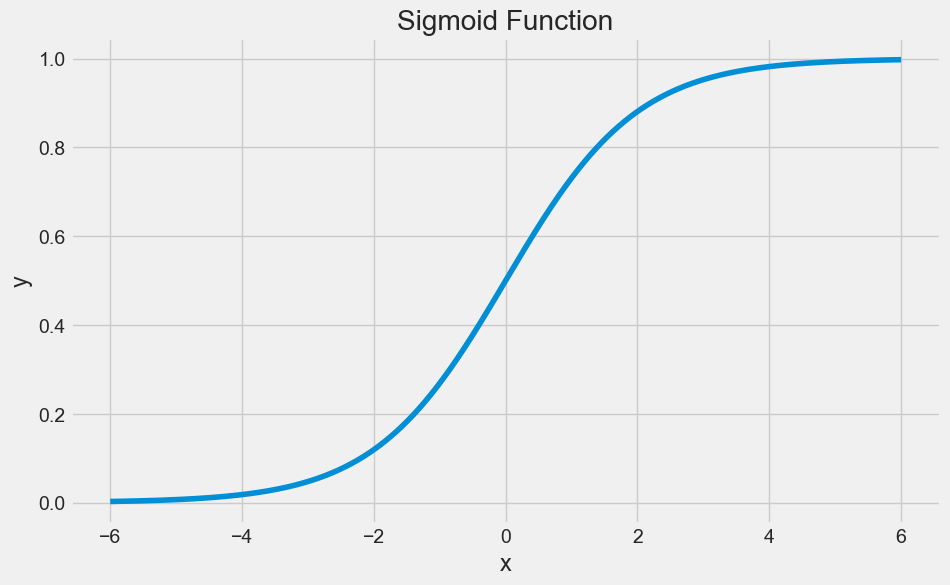
\includegraphics[keepaspectratio]{Logistic Regression_files/figure-pdf/cell-3-output-2.png}}

The logistic regression equation has a very similar representation like
linear regression. The difference is that the output value being
modelled is binary in nature.

\[\hat{p}=\frac{e^{\hat{\beta_0}+\hat{\beta_1}x_1}}{1+e^{\hat{\beta_0}+\hat{\beta_1}x_1}}\]

or

\[\hat{p}=\frac{1.0}{1.0+e^{-(\hat{\beta_0}+\hat{\beta_1}x_1)}}\]

\(\hat{\beta_0}\) is the estimated intercept term

\(\hat{\beta_1}\) is the estimated coefficient for \(x_1\)

\(\hat{p}\) is the predicted output with real value between 0 and 1. To
convert this to binary output of 0 or 1, this would either need to be
rounded to an integer value or a cutoff point be provided to specify the
class segregation point.

\subsection{Learning the Logistic Regression
Model}\label{learning-the-logistic-regression-model}

The coefficients (Beta values b) of the logistic regression algorithm
must be estimated from your training data. This is done using
\href{https://en.wikipedia.org/wiki/Maximum_likelihood_estimation}{maximum-likelihood
estimation}.

Maximum-likelihood estimation is a common learning algorithm used by a
variety of machine learning algorithms, although it does make
assumptions about the distribution of your data (more on this when we
talk about preparing your data).

The best coefficients should result in a model that would predict a
value very close to 1 (e.g.~male) for the default class and a value very
close to 0 (e.g.~female) for the other class. The intuition for
maximum-likelihood for logistic regression is that a search procedure
seeks values for the coefficients (Beta values) that maximize the
likelihood of the observed data. In other words, in MLE, we estimate the
parameter values (Beta values) which are the most likely to produce that
data at hand.

Here is an analogy to understand the idea behind Maximum Likelihood
Estimation (MLE). Let us say, you are listening to a song (data). You
are not aware of the singer (parameter) of the song. With just the
musical piece at hand, you try to guess the singer (parameter) who you
feel is the most likely (MLE) to have sung that song. Your are making a
maximum likelihood estimate! Out of all the singers (parameter space)
you have chosen them as the one who is the most likely to have sung that
song (data).

We are not going to go into the math of maximum likelihood. It is enough
to say that a minimization algorithm is used to optimize the best values
for the coefficients for your training data. This is often implemented
in practice using efficient numerical optimization algorithm (like the
Quasi-newton method).

When you are learning logistic, you can implement it yourself from
scratch using the much simpler gradient descent algorithm.

\subsection{Preparing Data for Logistic
Regression}\label{preparing-data-for-logistic-regression}

The assumptions made by logistic regression about the distribution and
relationships in your data are much the same as the assumptions made in
linear regression.

Much study has gone into defining these assumptions and precise
probabilistic and statistical language is used. My advice is to use
these as guidelines or rules of thumb and experiment with different data
preparation schemes.

Ultimately in predictive modeling machine learning projects you are
laser focused on making accurate predictions rather than interpreting
the results. As such, you can break some assumptions as long as the
model is robust and performs well.

\begin{itemize}
\tightlist
\item
  \textbf{Binary Output Variable:} This might be obvious as we have
  already mentioned it, but logistic regression is intended for binary
  (two-class) classification problems. It will predict the probability
  of an instance belonging to the default class, which can be snapped
  into a 0 or 1 classification.
\item
  \textbf{Remove Noise:} Logistic regression assumes no error in the
  output variable (y), consider removing outliers and possibly
  misclassified instances from your training data.
\item
  \textbf{Gaussian Distribution:} Logistic regression is a linear
  algorithm (with a non-linear transform on output). It does assume a
  linear relationship between the input variables with the output. Data
  transforms of your input variables that better expose this linear
  relationship can result in a more accurate model. For example, you can
  use log, root, Box-Cox and other univariate transforms to better
  expose this relationship.
\item
  \textbf{Remove Correlated Inputs:} Like linear regression, the model
  can overfit if you have multiple highly-correlated inputs. Consider
  calculating the pairwise correlations between all inputs and removing
  highly correlated inputs.
\item
  \textbf{Fail to Converge:} It is possible for the expected likelihood
  estimation process that learns the coefficients to fail to converge.
  This can happen if there are many highly correlated inputs in your
  data or the data is very sparse (e.g.~lots of zeros in your input
  data).
\end{itemize}

\section{Logistic Regression: Scikit-learn vs
Statsmodels}\label{logistic-regression-scikit-learn-vs-statsmodels}

Python gives us two ways to do logistic regression. Statsmodels offers
modeling from the perspective of statistics. Scikit-learn offers some of
the same models from the perspective of machine learning.

So we need to understand the difference between statistics and machine
learning! Statistics makes mathematically valid inferences about a
population based on sample data. Statistics answers the question, ``What
is the evidence that X is related to Y?'' Machine learning has the goal
of optimizing predictive accuracy rather than inference. Machine
learning answers the question, ``Given X, what prediction should we make
for Y?''

\section{Training a logistic regression
model}\label{training-a-logistic-regression-model}

Read the data on social network ads. The data shows if the person
purchased a product when targeted with an ad on social media. Fit a
logistic regression model to predict if a user will purchase the product
based on their characteristics such as age, gender and estimated salary.

\begin{Shaded}
\begin{Highlighting}[]
\OperatorTok{\%}\NormalTok{matplotlib inline}
\NormalTok{sns.set\_style(}\StringTok{\textquotesingle{}whitegrid\textquotesingle{}}\NormalTok{)}
\NormalTok{plt.style.use(}\StringTok{"fivethirtyeight"}\NormalTok{)}
\NormalTok{x }\OperatorTok{=}\NormalTok{ np.linspace(}\OperatorTok{{-}}\DecValTok{6}\NormalTok{, }\DecValTok{6}\NormalTok{, num}\OperatorTok{=}\DecValTok{1000}\NormalTok{)}
\NormalTok{plt.figure(figsize}\OperatorTok{=}\NormalTok{(}\DecValTok{6}\NormalTok{, }\DecValTok{4}\NormalTok{))}
\NormalTok{plt.plot(x, (}\DecValTok{1} \OperatorTok{/}\NormalTok{ (}\DecValTok{1} \OperatorTok{+}\NormalTok{ np.exp(}\OperatorTok{{-}}\NormalTok{x))))}
\NormalTok{plt.xlabel(}\StringTok{"x"}\NormalTok{)}
\NormalTok{plt.ylabel(}\StringTok{"y"}\NormalTok{)}
\NormalTok{plt.title(}\StringTok{"Sigmoid Function"}\NormalTok{)}\OperatorTok{;}
\end{Highlighting}
\end{Shaded}

\pandocbounded{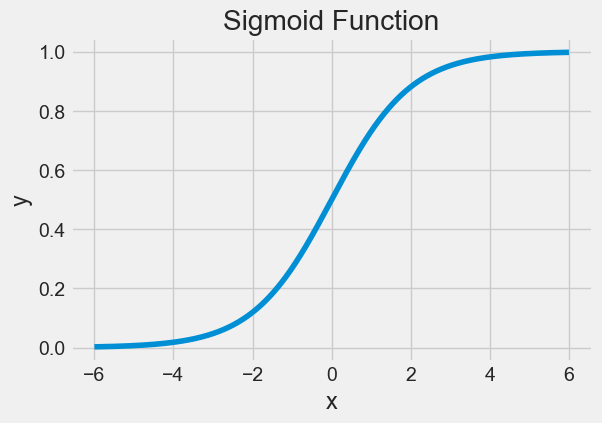
\includegraphics[keepaspectratio]{Logistic Regression_files/figure-pdf/cell-4-output-1.png}}

\section{Logistic Regression: Scikit-learn vs
Statsmodels}\label{logistic-regression-scikit-learn-vs-statsmodels-1}

Python gives us two ways to do logistic regression. Statsmodels offers
modeling from the perspective of statistics. Scikit-learn offers some of
the same models from the perspective of machine learning.

So we need to understand the difference between statistics and machine
learning! Statistics makes mathematically valid inferences about a
population based on sample data. Statistics answers the question, ``What
is the evidence that X is related to Y?'' Machine learning has the goal
of optimizing predictive accuracy rather than inference. Machine
learning answers the question, ``Given X, what prediction should we make
for Y?''

\begin{Shaded}
\begin{Highlighting}[]
\ImportTok{import}\NormalTok{ pandas }\ImportTok{as}\NormalTok{ pd}
\ImportTok{import}\NormalTok{ numpy }\ImportTok{as}\NormalTok{ np}
\ImportTok{import}\NormalTok{ seaborn }\ImportTok{as}\NormalTok{ sns}
\ImportTok{import}\NormalTok{ matplotlib.pyplot }\ImportTok{as}\NormalTok{ plt}
\ImportTok{import}\NormalTok{ statsmodels.formula.api }\ImportTok{as}\NormalTok{ sm}
\ImportTok{from}\NormalTok{ sklearn.metrics }\ImportTok{import}\NormalTok{ precision\_recall\_curve, roc\_curve, auc, accuracy\_score}
\ImportTok{from}\NormalTok{ sklearn.linear\_model }\ImportTok{import}\NormalTok{ LogisticRegression}
\end{Highlighting}
\end{Shaded}

Read the data on social network ads. The data shows if the person
purchased a product when targeted with an ad on social media. Fit a
logistic regression model to predict if a user will purchase the product
based on their characteristics such as age, gender and estimated salary.

\begin{Shaded}
\begin{Highlighting}[]
\NormalTok{train }\OperatorTok{=}\NormalTok{ pd.read\_csv(}\StringTok{\textquotesingle{}./Datasets/Social\_Network\_Ads\_train.csv\textquotesingle{}}\NormalTok{) }\CommentTok{\#Develop the model on train data}
\NormalTok{test }\OperatorTok{=}\NormalTok{ pd.read\_csv(}\StringTok{\textquotesingle{}./Datasets/Social\_Network\_Ads\_test.csv\textquotesingle{}}\NormalTok{) }\CommentTok{\#Test the model on test data}
\end{Highlighting}
\end{Shaded}

\begin{Shaded}
\begin{Highlighting}[]
\NormalTok{train.head()}
\end{Highlighting}
\end{Shaded}

\begin{longtable}[]{@{}llllll@{}}
\toprule\noalign{}
& User ID & Gender & Age & EstimatedSalary & Purchased \\
\midrule\noalign{}
\endhead
\bottomrule\noalign{}
\endlastfoot
0 & 15755018 & Male & 36 & 33000 & 0 \\
1 & 15697020 & Female & 39 & 61000 & 0 \\
2 & 15796351 & Male & 36 & 118000 & 1 \\
3 & 15665760 & Male & 39 & 122000 & 1 \\
4 & 15794661 & Female & 26 & 118000 & 0 \\
\end{longtable}

\subsection{Examining the Distribution of the Target Column, make sure
our target is not severely
imbalanced}\label{examining-the-distribution-of-the-target-column-make-sure-our-target-is-not-severely-imbalanced}

\begin{Shaded}
\begin{Highlighting}[]
\NormalTok{train.Purchased.value\_counts()}
\end{Highlighting}
\end{Shaded}

\begin{verbatim}
Purchased
0    194
1    106
Name: count, dtype: int64
\end{verbatim}

\begin{Shaded}
\begin{Highlighting}[]
\NormalTok{sns.countplot(x }\OperatorTok{=} \StringTok{\textquotesingle{}Purchased\textquotesingle{}}\NormalTok{,data }\OperatorTok{=}\NormalTok{ train)}\OperatorTok{;}
\end{Highlighting}
\end{Shaded}

\pandocbounded{\includegraphics[keepaspectratio]{Logistic Regression_files/figure-pdf/cell-9-output-1.png}}

\subsection{Fitting a linear
regression}\label{fitting-a-linear-regression}

\begin{Shaded}
\begin{Highlighting}[]
\NormalTok{sns.scatterplot(x }\OperatorTok{=} \StringTok{\textquotesingle{}Age\textquotesingle{}}\NormalTok{, y }\OperatorTok{=} \StringTok{\textquotesingle{}Purchased\textquotesingle{}}\NormalTok{, data }\OperatorTok{=}\NormalTok{ train, color }\OperatorTok{=} \StringTok{\textquotesingle{}orange\textquotesingle{}}\NormalTok{) }\CommentTok{\#Visualizing data}
\NormalTok{lm }\OperatorTok{=}\NormalTok{ sm.ols(formula }\OperatorTok{=} \StringTok{\textquotesingle{}Purchased\textasciitilde{}Age\textquotesingle{}}\NormalTok{, data }\OperatorTok{=}\NormalTok{ train).fit() }\CommentTok{\#Developing linear regression model}
\NormalTok{sns.lineplot(x }\OperatorTok{=} \StringTok{\textquotesingle{}Age\textquotesingle{}}\NormalTok{, y}\OperatorTok{=}\NormalTok{ lm.predict(train), data }\OperatorTok{=}\NormalTok{ train, color }\OperatorTok{=} \StringTok{\textquotesingle{}blue\textquotesingle{}}\NormalTok{) }\CommentTok{\#Visualizing model}
\end{Highlighting}
\end{Shaded}

\pandocbounded{\includegraphics[keepaspectratio]{Logistic Regression_files/figure-pdf/cell-10-output-1.png}}

\subsection{Logistic Regression with
Statsmodel}\label{logistic-regression-with-statsmodel}

\begin{Shaded}
\begin{Highlighting}[]
\NormalTok{sns.scatterplot(x }\OperatorTok{=} \StringTok{\textquotesingle{}Age\textquotesingle{}}\NormalTok{, y }\OperatorTok{=} \StringTok{\textquotesingle{}Purchased\textquotesingle{}}\NormalTok{, data }\OperatorTok{=}\NormalTok{ train, color }\OperatorTok{=} \StringTok{\textquotesingle{}orange\textquotesingle{}}\NormalTok{) }\CommentTok{\#Visualizing data}
\NormalTok{logit\_model }\OperatorTok{=}\NormalTok{ sm.logit(formula }\OperatorTok{=} \StringTok{\textquotesingle{}Purchased\textasciitilde{}Age\textquotesingle{}}\NormalTok{, data }\OperatorTok{=}\NormalTok{ train).fit() }\CommentTok{\#Developing logistic regression model}
\NormalTok{sns.lineplot(x }\OperatorTok{=} \StringTok{\textquotesingle{}Age\textquotesingle{}}\NormalTok{, y}\OperatorTok{=}\NormalTok{ logit\_model.predict(train), data }\OperatorTok{=}\NormalTok{ train, color }\OperatorTok{=} \StringTok{\textquotesingle{}blue\textquotesingle{}}\NormalTok{) }\CommentTok{\#Visualizing model}
\end{Highlighting}
\end{Shaded}

\begin{verbatim}
Optimization terminated successfully.
         Current function value: 0.430107
         Iterations 7
\end{verbatim}

\pandocbounded{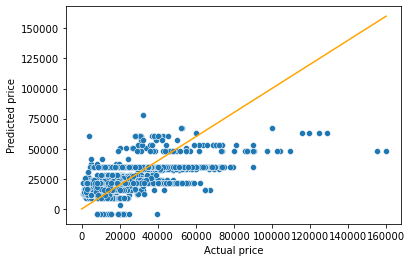
\includegraphics[keepaspectratio]{Logistic Regression_files/figure-pdf/cell-11-output-2.png}}

\begin{Shaded}
\begin{Highlighting}[]
\NormalTok{logit\_model.summary()}
\end{Highlighting}
\end{Shaded}

\begin{center}
\begin{tabular}{lclc}
\toprule
\textbf{Dep. Variable:}   &    Purchased     & \textbf{  No. Observations:  } &      300    \\
\textbf{Model:}           &      Logit       & \textbf{  Df Residuals:      } &      298    \\
\textbf{Method:}          &       MLE        & \textbf{  Df Model:          } &        1    \\
\textbf{Date:}            & Sun, 09 Feb 2025 & \textbf{  Pseudo R-squ.:     } &   0.3378    \\
\textbf{Time:}            &     18:28:20     & \textbf{  Log-Likelihood:    } &   -129.03   \\
\textbf{converged:}       &       True       & \textbf{  LL-Null:           } &   -194.85   \\
\textbf{Covariance Type:} &    nonrobust     & \textbf{  LLR p-value:       } & 1.805e-30   \\
\bottomrule
\end{tabular}
\begin{tabular}{lcccccc}
                   & \textbf{coef} & \textbf{std err} & \textbf{z} & \textbf{P$> |$z$|$} & \textbf{[0.025} & \textbf{0.975]}  \\
\midrule
\textbf{Intercept} &      -7.8102  &        0.885     &    -8.825  &         0.000        &       -9.545    &       -6.076     \\
\textbf{Age}       &       0.1842  &        0.022     &     8.449  &         0.000        &        0.141    &        0.227     \\
\bottomrule
\end{tabular}
%\caption{Logit Regression Results}
\end{center}

\begin{Shaded}
\begin{Highlighting}[]
\NormalTok{logit\_model\_gender }\OperatorTok{=}\NormalTok{ sm.logit(formula }\OperatorTok{=} \StringTok{\textquotesingle{}Purchased\textasciitilde{}Gender\textquotesingle{}}\NormalTok{, data }\OperatorTok{=}\NormalTok{ train).fit()}
\NormalTok{logit\_model\_gender.summary()}
\end{Highlighting}
\end{Shaded}

\begin{verbatim}
Optimization terminated successfully.
         Current function value: 0.648804
         Iterations 4
\end{verbatim}

\begin{center}
\begin{tabular}{lclc}
\toprule
\textbf{Dep. Variable:}   &    Purchased     & \textbf{  No. Observations:  } &      300    \\
\textbf{Model:}           &      Logit       & \textbf{  Df Residuals:      } &      298    \\
\textbf{Method:}          &       MLE        & \textbf{  Df Model:          } &        1    \\
\textbf{Date:}            & Sun, 09 Feb 2025 & \textbf{  Pseudo R-squ.:     } &  0.001049   \\
\textbf{Time:}            &     18:28:20     & \textbf{  Log-Likelihood:    } &   -194.64   \\
\textbf{converged:}       &       True       & \textbf{  LL-Null:           } &   -194.85   \\
\textbf{Covariance Type:} &    nonrobust     & \textbf{  LLR p-value:       } &   0.5225    \\
\bottomrule
\end{tabular}
\begin{tabular}{lcccccc}
                        & \textbf{coef} & \textbf{std err} & \textbf{z} & \textbf{P$> |$z$|$} & \textbf{[0.025} & \textbf{0.975]}  \\
\midrule
\textbf{Intercept}      &      -0.5285  &        0.168     &    -3.137  &         0.002        &       -0.859    &       -0.198     \\
\textbf{Gender[T.Male]} &      -0.1546  &        0.242     &    -0.639  &         0.523        &       -0.629    &        0.319     \\
\bottomrule
\end{tabular}
%\caption{Logit Regression Results}
\end{center}

\begin{Shaded}
\begin{Highlighting}[]
\CommentTok{\# Predicted probabilities}
\NormalTok{predicted\_probabilities }\OperatorTok{=}\NormalTok{ logit\_model.predict(train)}
\NormalTok{predicted\_probabilities}
\end{Highlighting}
\end{Shaded}

\begin{verbatim}
0      0.235159
1      0.348227
2      0.235159
3      0.348227
4      0.046473
         ...   
295    0.737081
296    0.481439
297    0.065810
298    0.829688
299    0.150336
Length: 300, dtype: float64
\end{verbatim}

\begin{Shaded}
\begin{Highlighting}[]
\CommentTok{\# Predicted classes (binary outcome, 0 or 1)}
\NormalTok{predicted\_classes }\OperatorTok{=}\NormalTok{ (predicted\_probabilities }\OperatorTok{\textgreater{}} \FloatTok{0.5}\NormalTok{).astype(}\BuiltInTok{int}\NormalTok{)}
\NormalTok{predicted\_classes}
\end{Highlighting}
\end{Shaded}

\begin{verbatim}
0      0
1      0
2      0
3      0
4      0
      ..
295    1
296    0
297    0
298    1
299    0
Length: 300, dtype: int32
\end{verbatim}

\begin{Shaded}
\begin{Highlighting}[]
\CommentTok{\#Function to compute confusion matrix and prediction accuracy on training data}
\KeywordTok{def}\NormalTok{ confusion\_matrix\_train(model,cutoff}\OperatorTok{=}\FloatTok{0.5}\NormalTok{):}
    \CommentTok{\# Confusion matrix}
\NormalTok{    cm\_df }\OperatorTok{=}\NormalTok{ pd.DataFrame(model.pred\_table(threshold }\OperatorTok{=}\NormalTok{ cutoff))}
    \CommentTok{\#Formatting the confusion matrix}
\NormalTok{    cm\_df.columns }\OperatorTok{=}\NormalTok{ [}\StringTok{\textquotesingle{}Predicted 0\textquotesingle{}}\NormalTok{, }\StringTok{\textquotesingle{}Predicted 1\textquotesingle{}}\NormalTok{] }
\NormalTok{    cm\_df }\OperatorTok{=}\NormalTok{ cm\_df.rename(index}\OperatorTok{=}\NormalTok{\{}\DecValTok{0}\NormalTok{: }\StringTok{\textquotesingle{}Actual 0\textquotesingle{}}\NormalTok{,}\DecValTok{1}\NormalTok{: }\StringTok{\textquotesingle{}Actual 1\textquotesingle{}}\NormalTok{\})}
\NormalTok{    cm }\OperatorTok{=}\NormalTok{ np.array(cm\_df)}
    \CommentTok{\# Calculate the accuracy}
\NormalTok{    accuracy }\OperatorTok{=}\NormalTok{ (cm[}\DecValTok{0}\NormalTok{,}\DecValTok{0}\NormalTok{]}\OperatorTok{+}\NormalTok{cm[}\DecValTok{1}\NormalTok{,}\DecValTok{1}\NormalTok{])}\OperatorTok{/}\NormalTok{cm.}\BuiltInTok{sum}\NormalTok{()}
\NormalTok{    sns.heatmap(cm\_df, annot}\OperatorTok{=}\VariableTok{True}\NormalTok{, cmap}\OperatorTok{=}\StringTok{\textquotesingle{}Blues\textquotesingle{}}\NormalTok{, fmt}\OperatorTok{=}\StringTok{\textquotesingle{}g\textquotesingle{}}\NormalTok{)}
\NormalTok{    plt.ylabel(}\StringTok{"Actual Values"}\NormalTok{)}
\NormalTok{    plt.xlabel(}\StringTok{"Predicted Values"}\NormalTok{)}
    \BuiltInTok{print}\NormalTok{(}\StringTok{"Classification accuracy = }\SpecialCharTok{\{:.1\%\}}\StringTok{"}\NormalTok{.}\BuiltInTok{format}\NormalTok{(accuracy))}
\end{Highlighting}
\end{Shaded}

\begin{Shaded}
\begin{Highlighting}[]
\NormalTok{cm }\OperatorTok{=}\NormalTok{ confusion\_matrix\_train(logit\_model)}
\end{Highlighting}
\end{Shaded}

\begin{verbatim}
Classification accuracy = 83.3%
\end{verbatim}

\pandocbounded{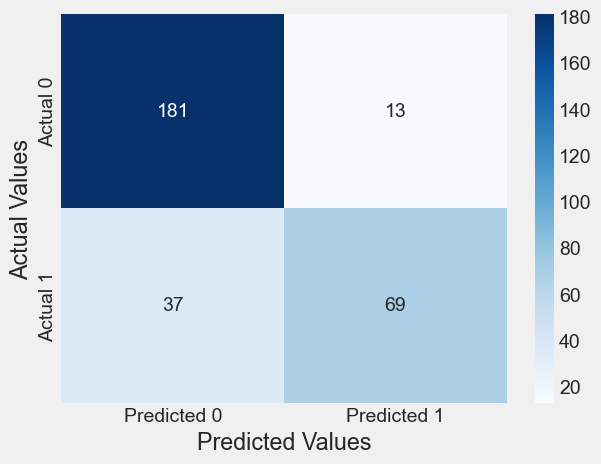
\includegraphics[keepaspectratio]{Logistic Regression_files/figure-pdf/cell-17-output-2.png}}

\begin{Shaded}
\begin{Highlighting}[]
\CommentTok{\# change the cutoff to 0.3}
\NormalTok{cm }\OperatorTok{=}\NormalTok{ confusion\_matrix\_train(logit\_model, }\FloatTok{0.3}\NormalTok{)}
\end{Highlighting}
\end{Shaded}

\begin{verbatim}
Classification accuracy = 73.7%
\end{verbatim}

\pandocbounded{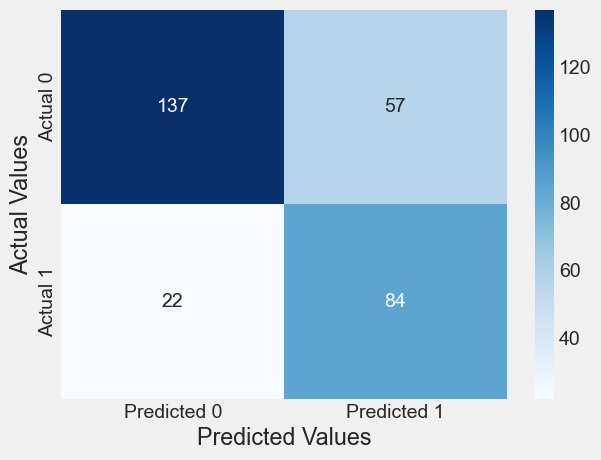
\includegraphics[keepaspectratio]{Logistic Regression_files/figure-pdf/cell-18-output-2.png}}

\begin{Shaded}
\begin{Highlighting}[]
\CommentTok{\# increase the cutoff to 0.7}
\NormalTok{cm }\OperatorTok{=}\NormalTok{ confusion\_matrix\_train(logit\_model, }\FloatTok{0.8}\NormalTok{)}
\end{Highlighting}
\end{Shaded}

\begin{verbatim}
Classification accuracy = 74.7%
\end{verbatim}

\pandocbounded{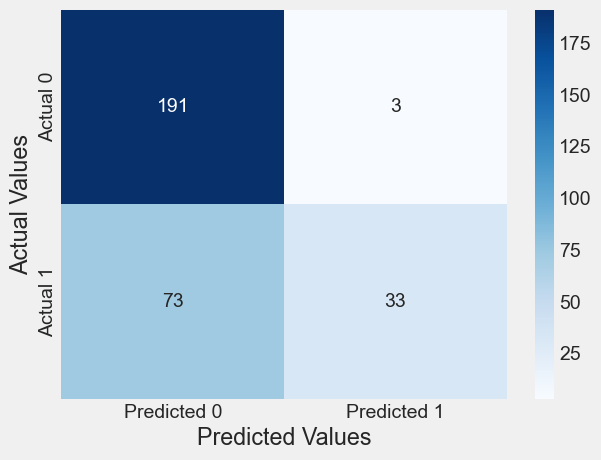
\includegraphics[keepaspectratio]{Logistic Regression_files/figure-pdf/cell-19-output-2.png}}

\textbf{Making prediction on test set and output the model's
performance}

\begin{Shaded}
\begin{Highlighting}[]
\CommentTok{\# Predicted probabilities}
\NormalTok{predicted\_probabilities }\OperatorTok{=}\NormalTok{ logit\_model.predict(test)}
\end{Highlighting}
\end{Shaded}

\begin{Shaded}
\begin{Highlighting}[]
\CommentTok{\# Predicted classes (binary outcome, 0 or 1)}
\NormalTok{predicted\_classes }\OperatorTok{=}\NormalTok{ (predicted\_probabilities }\OperatorTok{\textgreater{}} \FloatTok{0.5}\NormalTok{).astype(}\BuiltInTok{int}\NormalTok{)}
\NormalTok{predicted\_classes}
\end{Highlighting}
\end{Shaded}

\begin{verbatim}
0     0
1     0
2     0
3     0
4     0
     ..
95    1
96    1
97    1
98    0
99    1
Length: 100, dtype: int32
\end{verbatim}

\begin{Shaded}
\begin{Highlighting}[]
\ImportTok{from}\NormalTok{ sklearn.metrics }\ImportTok{import}\NormalTok{ confusion\_matrix}
\end{Highlighting}
\end{Shaded}

\begin{Shaded}
\begin{Highlighting}[]
\NormalTok{confusion\_mat }\OperatorTok{=}\NormalTok{ confusion\_matrix(test.Purchased, predicted\_classes)}
\CommentTok{\# Define labels for the confusion matrix}
\NormalTok{labels }\OperatorTok{=}\NormalTok{ [}\StringTok{\textquotesingle{}Actual Negative\textquotesingle{}}\NormalTok{, }\StringTok{\textquotesingle{}Actual Positive\textquotesingle{}}\NormalTok{]}
\CommentTok{\# Create a formatted confusion matrix}
\NormalTok{formatted\_confusion\_mat }\OperatorTok{=}\NormalTok{ pd.DataFrame(confusion\_mat, index}\OperatorTok{=}\NormalTok{labels, columns}\OperatorTok{=}\NormalTok{[}\SpecialStringTok{f\textquotesingle{}Predicted }\SpecialCharTok{\{}\NormalTok{label}\SpecialCharTok{\}}\SpecialStringTok{\textquotesingle{}} \ControlFlowTok{for}\NormalTok{ label }\KeywordTok{in}\NormalTok{ labels])}

\BuiltInTok{print}\NormalTok{(}\StringTok{"Confusion Matrix:"}\NormalTok{)}
\BuiltInTok{print}\NormalTok{(formatted\_confusion\_mat)}
\end{Highlighting}
\end{Shaded}

\begin{verbatim}
Confusion Matrix:
                 Predicted Actual Negative  Predicted Actual Positive
Actual Negative                         58                          5
Actual Positive                          9                         28
\end{verbatim}

\subsection{Logistic Regression with
Sklearn}\label{logistic-regression-with-sklearn}

\begin{Shaded}
\begin{Highlighting}[]
\NormalTok{X\_train }\OperatorTok{=}\NormalTok{ train[[}\StringTok{\textquotesingle{}Age\textquotesingle{}}\NormalTok{]]}
\NormalTok{y\_train }\OperatorTok{=}\NormalTok{ train[}\StringTok{\textquotesingle{}Purchased\textquotesingle{}}\NormalTok{]}

\NormalTok{X\_test }\OperatorTok{=}\NormalTok{ test[[}\StringTok{\textquotesingle{}Age\textquotesingle{}}\NormalTok{]]}
\NormalTok{y\_test }\OperatorTok{=}\NormalTok{ test[}\StringTok{\textquotesingle{}Purchased\textquotesingle{}}\NormalTok{]}
\end{Highlighting}
\end{Shaded}

\begin{Shaded}
\begin{Highlighting}[]
\CommentTok{\# turn off regularization}
\NormalTok{skn\_model }\OperatorTok{=}\NormalTok{ LogisticRegression(penalty}\OperatorTok{=}\VariableTok{None}\NormalTok{)}
\end{Highlighting}
\end{Shaded}

\begin{Shaded}
\begin{Highlighting}[]
\NormalTok{skn\_model.fit(X\_train, y\_train)}
\end{Highlighting}
\end{Shaded}

\begin{verbatim}
LogisticRegression(penalty=None)
\end{verbatim}

\begin{Shaded}
\begin{Highlighting}[]
\CommentTok{\# Note that in sklearn, .predict returns the classes directly, with 0.5 threshold}
\NormalTok{y\_pred\_test }\OperatorTok{=}\NormalTok{ skn\_model.predict(X\_test)}
\NormalTok{y\_pred\_test}
\end{Highlighting}
\end{Shaded}

\begin{verbatim}
array([0, 0, 0, 0, 0, 1, 1, 1, 1, 0, 0, 0, 0, 0, 0, 1, 0, 0, 0, 0, 0, 0,
       0, 0, 0, 0, 0, 0, 0, 0, 0, 0, 0, 0, 0, 0, 0, 0, 0, 0, 0, 1, 0, 0,
       0, 0, 0, 0, 0, 0, 1, 1, 1, 0, 1, 0, 1, 0, 1, 1, 0, 1, 1, 1, 1, 0,
       1, 0, 0, 0, 1, 1, 0, 0, 0, 1, 0, 0, 1, 1, 0, 0, 1, 0, 1, 0, 0, 1,
       0, 0, 0, 0, 1, 1, 1, 1, 1, 1, 0, 1], dtype=int64)
\end{verbatim}

\begin{Shaded}
\begin{Highlighting}[]
\CommentTok{\# To return the prediction probabilities, we need .predict\_proba}
\CommentTok{\# \# probs\_y is a 2{-}D array of probability of being labeled as 0 (first column of array) vs 1 (2nd column in array)}
\NormalTok{y\_pred\_probs }\OperatorTok{=}\NormalTok{ skn\_model.predict\_proba(X\_test)}
\NormalTok{y\_pred\_probs[:}\DecValTok{5}\NormalTok{]}
\end{Highlighting}
\end{Shaded}

\begin{verbatim}
array([[0.79634123, 0.20365877],
       [0.95352574, 0.04647426],
       [0.944647  , 0.055353  ],
       [0.8717078 , 0.1282922 ],
       [0.92191865, 0.07808135]])
\end{verbatim}

\begin{Shaded}
\begin{Highlighting}[]
\NormalTok{cm}\OperatorTok{=}\NormalTok{confusion\_matrix(y\_test,y\_pred\_test)}
\CommentTok{\#plt.figure(figsize=(4,4))}
\NormalTok{plt.title(}\StringTok{"Confusion Matrix on test data"}\NormalTok{)}
\NormalTok{sns.heatmap(cm, annot}\OperatorTok{=}\VariableTok{True}\NormalTok{,fmt}\OperatorTok{=}\StringTok{\textquotesingle{}d\textquotesingle{}}\NormalTok{, cmap}\OperatorTok{=}\StringTok{\textquotesingle{}Blues\textquotesingle{}}\NormalTok{)}
\NormalTok{plt.ylabel(}\StringTok{"Actual Values"}\NormalTok{)}
\NormalTok{plt.xlabel(}\StringTok{"Predicted Values"}\NormalTok{)}
\end{Highlighting}
\end{Shaded}

\begin{verbatim}
Text(0.5, 5.183333333333314, 'Predicted Values')
\end{verbatim}

\pandocbounded{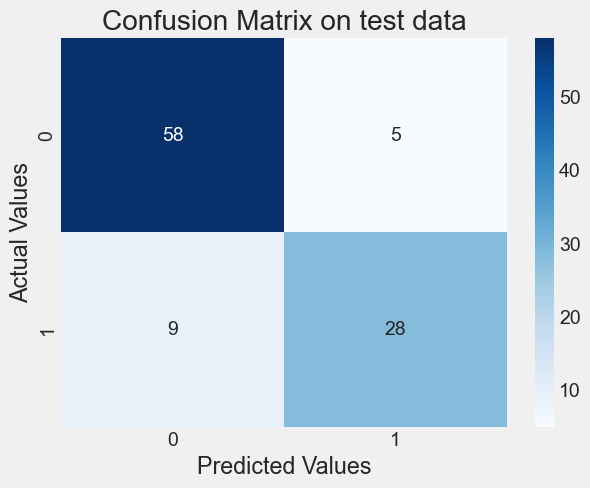
\includegraphics[keepaspectratio]{Logistic Regression_files/figure-pdf/cell-29-output-2.png}}

\begin{Shaded}
\begin{Highlighting}[]
\ImportTok{from}\NormalTok{ sklearn.metrics }\ImportTok{import}\NormalTok{ accuracy\_score}
\BuiltInTok{print}\NormalTok{(}\StringTok{"Accuracy:"}\NormalTok{, accuracy\_score(y\_test, y\_pred\_test))}
\ImportTok{from}\NormalTok{ sklearn.metrics }\ImportTok{import}\NormalTok{ precision\_score}
\BuiltInTok{print}\NormalTok{(}\StringTok{"Precision:"}\NormalTok{, precision\_score(y\_test, y\_pred\_test))}
\ImportTok{from}\NormalTok{ sklearn.metrics }\ImportTok{import}\NormalTok{ recall\_score}
\BuiltInTok{print}\NormalTok{(}\StringTok{"Recall:"}\NormalTok{, recall\_score(y\_test, y\_pred\_test))}
\ImportTok{from}\NormalTok{ sklearn.metrics }\ImportTok{import}\NormalTok{ f1\_score}
\BuiltInTok{print}\NormalTok{(}\StringTok{"F1 score:"}\NormalTok{,  f1\_score(y\_test, y\_pred\_test))}
\end{Highlighting}
\end{Shaded}

\begin{verbatim}
Accuracy: 0.86
Precision: 0.8484848484848485
Recall: 0.7567567567567568
F1 score: 0.8
\end{verbatim}

\subsection{Changing the default
threshold}\label{changing-the-default-threshold}

\begin{Shaded}
\begin{Highlighting}[]
\NormalTok{new\_threshold }\OperatorTok{=} \FloatTok{0.3}
\end{Highlighting}
\end{Shaded}

\begin{Shaded}
\begin{Highlighting}[]
\NormalTok{predicted\_classes\_new\_threshold }\OperatorTok{=}\NormalTok{ (y\_pred\_probs }\OperatorTok{\textgreater{}}\NormalTok{ new\_threshold).astype(}\BuiltInTok{int}\NormalTok{)}
\NormalTok{predicted\_classes\_new\_threshold[:}\DecValTok{5}\NormalTok{]}
\end{Highlighting}
\end{Shaded}

\begin{verbatim}
array([[1, 0],
       [1, 0],
       [1, 0],
       [1, 0],
       [1, 0]])
\end{verbatim}

\begin{Shaded}
\begin{Highlighting}[]
\NormalTok{confusion\_mat\_new\_threshold }\OperatorTok{=}\NormalTok{ confusion\_matrix(y\_test, predicted\_classes\_new\_threshold[:, }\DecValTok{1}\NormalTok{])}
\BuiltInTok{print}\NormalTok{(}\StringTok{"Confusion Matrix (Threshold ="}\NormalTok{, new\_threshold, }\StringTok{"):"}\NormalTok{)}
\BuiltInTok{print}\NormalTok{(confusion\_mat\_new\_threshold)}
\ImportTok{from}\NormalTok{ sklearn.metrics }\ImportTok{import}\NormalTok{ accuracy\_score}
\BuiltInTok{print}\NormalTok{(}\StringTok{"Accuracy:"}\NormalTok{, accuracy\_score(y\_test, predicted\_classes\_new\_threshold[:, }\DecValTok{1}\NormalTok{]))}
\ImportTok{from}\NormalTok{ sklearn.metrics }\ImportTok{import}\NormalTok{ precision\_score}
\BuiltInTok{print}\NormalTok{(}\StringTok{"Precision:"}\NormalTok{, precision\_score(y\_test, predicted\_classes\_new\_threshold[:, }\DecValTok{1}\NormalTok{]))}
\ImportTok{from}\NormalTok{ sklearn.metrics }\ImportTok{import}\NormalTok{ recall\_score}
\BuiltInTok{print}\NormalTok{(}\StringTok{"Recall:"}\NormalTok{, recall\_score(y\_test, predicted\_classes\_new\_threshold[:, }\DecValTok{1}\NormalTok{]))}
\ImportTok{from}\NormalTok{ sklearn.metrics }\ImportTok{import}\NormalTok{ f1\_score}
\BuiltInTok{print}\NormalTok{(}\StringTok{"F1 score:"}\NormalTok{,  f1\_score(y\_test, predicted\_classes\_new\_threshold[:, }\DecValTok{1}\NormalTok{]))}
\end{Highlighting}
\end{Shaded}

\begin{verbatim}
Confusion Matrix (Threshold = 0.3 ):
[[44 19]
 [ 7 30]]
Accuracy: 0.74
Precision: 0.6122448979591837
Recall: 0.8108108108108109
F1 score: 0.6976744186046512
\end{verbatim}

\section{Performance Measurement}\label{performance-measurement}

We have already seen the confusion matrix, and classification accuracy.
Now, let us see some other useful performance metrics that can be
computed from the confusion matrix. The metrics below are computed for
the confusion matrix immediately above this section \emph{(or the
confusion matrix on test data corresponding to the model
\texttt{logit\_model\_diabetes})}.

\subsection{Precision-recall}\label{precision-recall}

\textbf{Precision} measures the accuracy of positive predictions. Also
called the \texttt{precision} of the classifier

\[\textrm{precision} = \frac{\textrm{True Positives}}{\textrm{True Positives} + \textrm{False Positives}}\]

==\textgreater{} \texttt{70.13\%}

\texttt{Precision} is typically used with \texttt{recall}
(\texttt{Sensitivity} or \texttt{True\ Positive\ Rate}). The ratio of
positive instances that are correctly detected by the classifier.

\(\textrm{recall} = \frac{\textrm{True Positives}}{\textrm{True Positives} + \textrm{False Negatives}}\)
==\textgreater{} \texttt{88.52\%}

\textbf{Precision / Recall Tradeoff}: Increasing precision reduces
recall and vice versa.

\textbf{Visualize the precision-recall curve for the model
\texttt{logit\_model\_diabetes}}.

\begin{Shaded}
\begin{Highlighting}[]
\NormalTok{train}
\end{Highlighting}
\end{Shaded}

\begin{longtable}[]{@{}llllll@{}}
\toprule\noalign{}
& User ID & Gender & Age & EstimatedSalary & Purchased \\
\midrule\noalign{}
\endhead
\bottomrule\noalign{}
\endlastfoot
0 & 15755018 & Male & 36 & 33000 & 0 \\
1 & 15697020 & Female & 39 & 61000 & 0 \\
2 & 15796351 & Male & 36 & 118000 & 1 \\
3 & 15665760 & Male & 39 & 122000 & 1 \\
4 & 15794661 & Female & 26 & 118000 & 0 \\
... & ... & ... & ... & ... & ... \\
295 & 15724536 & Female & 48 & 96000 & 1 \\
296 & 15701537 & Male & 42 & 149000 & 1 \\
297 & 15807481 & Male & 28 & 79000 & 0 \\
298 & 15603942 & Female & 51 & 134000 & 0 \\
299 & 15690188 & Female & 33 & 28000 & 0 \\
\end{longtable}

\begin{Shaded}
\begin{Highlighting}[]
\NormalTok{y}\OperatorTok{=}\NormalTok{train.Purchased}
\NormalTok{ypred }\OperatorTok{=}\NormalTok{ lm.predict(train)}
\NormalTok{p, r, thresholds }\OperatorTok{=}\NormalTok{ precision\_recall\_curve(y, ypred)}
\KeywordTok{def}\NormalTok{ plot\_precision\_recall\_vs\_threshold(precisions, recalls, thresholds):}
\NormalTok{    plt.figure(figsize}\OperatorTok{=}\NormalTok{(}\DecValTok{8}\NormalTok{, }\DecValTok{8}\NormalTok{))}
\NormalTok{    plt.title(}\StringTok{"Precision and Recall Scores as a function of the decision threshold"}\NormalTok{)}
\NormalTok{    plt.plot(thresholds, precisions[:}\OperatorTok{{-}}\DecValTok{1}\NormalTok{], }\StringTok{"b{-}{-}"}\NormalTok{, label}\OperatorTok{=}\StringTok{"Precision"}\NormalTok{)}
\NormalTok{    plt.plot(thresholds, recalls[:}\OperatorTok{{-}}\DecValTok{1}\NormalTok{], }\StringTok{"g{-}"}\NormalTok{, label}\OperatorTok{=}\StringTok{"Recall"}\NormalTok{)}
\NormalTok{    plt.ylabel(}\StringTok{"Score"}\NormalTok{)}
\NormalTok{    plt.xlabel(}\StringTok{"Decision Threshold"}\NormalTok{)}
\NormalTok{    plt.legend(loc}\OperatorTok{=}\StringTok{\textquotesingle{}best\textquotesingle{}}\NormalTok{)}
\NormalTok{    plt.legend()}
\NormalTok{plot\_precision\_recall\_vs\_threshold(p, r, thresholds)}
\end{Highlighting}
\end{Shaded}

\pandocbounded{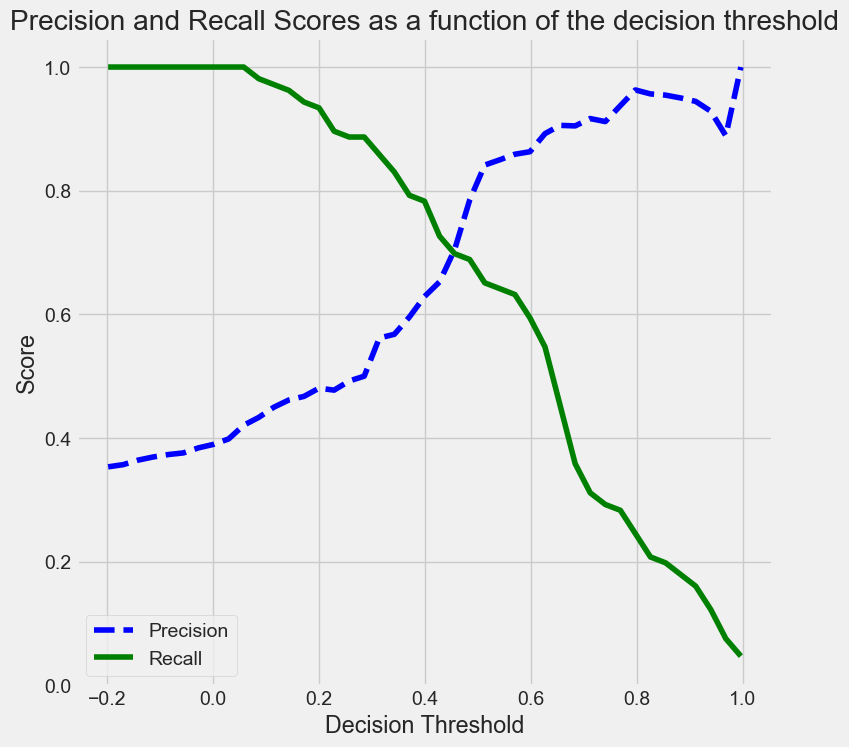
\includegraphics[keepaspectratio]{Logistic Regression_files/figure-pdf/cell-35-output-1.png}}

As the decision threshold probability increases, the precision
increases, while the recall decreases.

\textbf{Q:} How are the values of the \texttt{thresholds} chosen to make
the precision-recall curve?

\textbf{Hint:} Look at the documentation for
\href{https://scikit-learn.org/stable/modules/generated/sklearn.metrics.precision_recall_curve.html}{\texttt{precision\_recall\_curve}}.

\subsection{The Receiver Operating Characteristics (ROC)
Curve}\label{the-receiver-operating-characteristics-roc-curve}

A \textbf{ROC(Receiver Operator Characteristic Curve)} is a plot of
sensitivity (True Positive Rate) on the y axis against (1−specificity)
(False Positive Rate) on the x axis for varying values of the threshold
t. The 45° diagonal line connecting (0,0) to (1,1) is the ROC curve
corresponding to random chance. The ROC curve for the gold standard is
the line connecting (0,0) to (0,1) and (0,1) to (1,1).

\begin{verbatim}
<IPython.core.display.Image object>
\end{verbatim}

\begin{verbatim}
<IPython.core.display.Image object>
\end{verbatim}

An animation to demonstrate how an ROC curve relates to sensitivity and
specificity for all possible cutoffs
(\href{https://github.com/dariyasydykova/open_projects/blob/master/ROC_animation/animations/ROC.gif}{Source})

\textbf{High Threshold:}

\begin{itemize}
\tightlist
\item
  High specificity
\item
  Low sensitivity
\end{itemize}

\textbf{Low Threshold}

\begin{itemize}
\tightlist
\item
  Low specificity
\item
  High sensitivity
\end{itemize}

The area under ROC is called \emph{Area Under the Curve(AUC)}. AUC gives
the rate of successful classification by the logistic model. To get a
more in-depth idea of what a ROC-AUC curve is and how is it calculated,
here is a good blog
\href{https://www.analyticsvidhya.com/blog/2020/06/auc-roc-curve-machine-learning/}{link}.

Here is good
\href{https://developers.google.com/machine-learning/crash-course/classification/roc-and-auc}{post}
by google developers on interpreting ROC-AUC, and its advantages /
disadvantages.

\textbf{Visualize the ROC curve and compute the ROC-AUC for the model
\texttt{logit\_model\_diabetes}}.

\begin{Shaded}
\begin{Highlighting}[]
\NormalTok{y}\OperatorTok{=}\NormalTok{train.Purchased}
\NormalTok{ypred }\OperatorTok{=}\NormalTok{ lm.predict(train)}
\NormalTok{fpr, tpr, auc\_thresholds }\OperatorTok{=}\NormalTok{ roc\_curve(y, ypred)}
\BuiltInTok{print}\NormalTok{(auc(fpr, tpr))}\CommentTok{\# AUC of ROC}
\KeywordTok{def}\NormalTok{ plot\_roc\_curve(fpr, tpr, label}\OperatorTok{=}\VariableTok{None}\NormalTok{):}
\NormalTok{    plt.figure(figsize}\OperatorTok{=}\NormalTok{(}\DecValTok{8}\NormalTok{,}\DecValTok{8}\NormalTok{))}
\NormalTok{    plt.title(}\StringTok{\textquotesingle{}ROC Curve\textquotesingle{}}\NormalTok{)}
\NormalTok{    plt.plot(fpr, tpr, linewidth}\OperatorTok{=}\DecValTok{2}\NormalTok{, label}\OperatorTok{=}\NormalTok{label)}
\NormalTok{    plt.plot([}\DecValTok{0}\NormalTok{, }\DecValTok{1}\NormalTok{], [}\DecValTok{0}\NormalTok{, }\DecValTok{1}\NormalTok{], }\StringTok{\textquotesingle{}k{-}{-}\textquotesingle{}}\NormalTok{)}
\NormalTok{    plt.axis([}\OperatorTok{{-}}\FloatTok{0.005}\NormalTok{, }\DecValTok{1}\NormalTok{, }\DecValTok{0}\NormalTok{, }\FloatTok{1.005}\NormalTok{])}
\NormalTok{    plt.xticks(np.arange(}\DecValTok{0}\NormalTok{,}\DecValTok{1}\NormalTok{, }\FloatTok{0.05}\NormalTok{), rotation}\OperatorTok{=}\DecValTok{90}\NormalTok{)}
\NormalTok{    plt.xlabel(}\StringTok{"False Positive Rate"}\NormalTok{)}
\NormalTok{    plt.ylabel(}\StringTok{"True Positive Rate (Recall)"}\NormalTok{)}

\NormalTok{fpr, tpr, auc\_thresholds }\OperatorTok{=}\NormalTok{ roc\_curve(y, ypred)}
\NormalTok{plot\_roc\_curve(fpr, tpr)}
\end{Highlighting}
\end{Shaded}

\begin{verbatim}
0.8593901964598327
\end{verbatim}

\pandocbounded{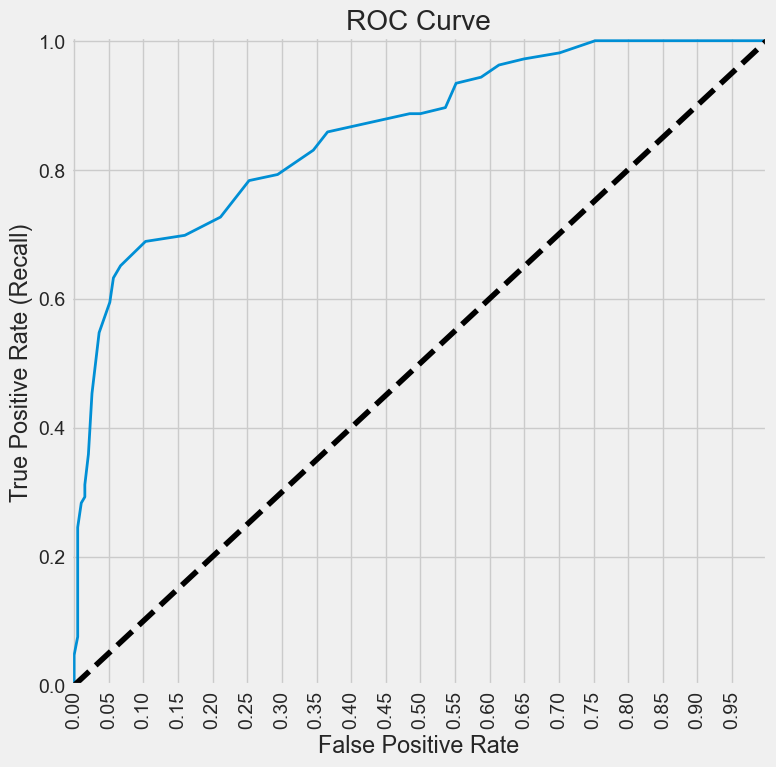
\includegraphics[keepaspectratio]{Logistic Regression_files/figure-pdf/cell-38-output-2.png}}

\textbf{Q:} How are the values of the \texttt{auc\_thresholds} chosen to
make the ROC curve? Why does it look like a step function?

Below is a function that prints the confusion matrix along with all the
performance metrics we discussed above for a given decision threshold
probability, on train / test data. Note that ROC-AUC does not depend on
a decision threshold probability.

\begin{Shaded}
\begin{Highlighting}[]
\CommentTok{\#Function to compute confusion matrix and prediction accuracy on test/train data}
\KeywordTok{def}\NormalTok{ confusion\_matrix\_data(data,actual\_values,model,cutoff}\OperatorTok{=}\FloatTok{0.5}\NormalTok{):}
\CommentTok{\#Predict the values using the Logit model}
\NormalTok{    pred\_values }\OperatorTok{=}\NormalTok{ model.predict(data)}
\CommentTok{\# Specify the bins}
\NormalTok{    bins}\OperatorTok{=}\NormalTok{np.array([}\DecValTok{0}\NormalTok{,cutoff,}\DecValTok{1}\NormalTok{])}
\CommentTok{\#Confusion matrix}
\NormalTok{    cm }\OperatorTok{=}\NormalTok{ np.histogram2d(actual\_values, pred\_values, bins}\OperatorTok{=}\NormalTok{bins)[}\DecValTok{0}\NormalTok{]}
\NormalTok{    cm\_df }\OperatorTok{=}\NormalTok{ pd.DataFrame(cm)}
\NormalTok{    cm\_df.columns }\OperatorTok{=}\NormalTok{ [}\StringTok{\textquotesingle{}Predicted 0\textquotesingle{}}\NormalTok{,}\StringTok{\textquotesingle{}Predicted 1\textquotesingle{}}\NormalTok{]}
\NormalTok{    cm\_df }\OperatorTok{=}\NormalTok{ cm\_df.rename(index}\OperatorTok{=}\NormalTok{\{}\DecValTok{0}\NormalTok{: }\StringTok{\textquotesingle{}Actual 0\textquotesingle{}}\NormalTok{,}\DecValTok{1}\NormalTok{:}\StringTok{\textquotesingle{}Actual 1\textquotesingle{}}\NormalTok{\})}
\CommentTok{\# Calculate the accuracy}
\NormalTok{    accuracy }\OperatorTok{=}\NormalTok{ (cm[}\DecValTok{0}\NormalTok{,}\DecValTok{0}\NormalTok{]}\OperatorTok{+}\NormalTok{cm[}\DecValTok{1}\NormalTok{,}\DecValTok{1}\NormalTok{])}\OperatorTok{/}\NormalTok{cm.}\BuiltInTok{sum}\NormalTok{()}
\NormalTok{    fnr }\OperatorTok{=}\NormalTok{ (cm[}\DecValTok{1}\NormalTok{,}\DecValTok{0}\NormalTok{])}\OperatorTok{/}\NormalTok{(cm[}\DecValTok{1}\NormalTok{,}\DecValTok{0}\NormalTok{]}\OperatorTok{+}\NormalTok{cm[}\DecValTok{1}\NormalTok{,}\DecValTok{1}\NormalTok{])}
\NormalTok{    precision }\OperatorTok{=}\NormalTok{ (cm[}\DecValTok{1}\NormalTok{,}\DecValTok{1}\NormalTok{])}\OperatorTok{/}\NormalTok{(cm[}\DecValTok{0}\NormalTok{,}\DecValTok{1}\NormalTok{]}\OperatorTok{+}\NormalTok{cm[}\DecValTok{1}\NormalTok{,}\DecValTok{1}\NormalTok{])}
\NormalTok{    fpr }\OperatorTok{=}\NormalTok{ (cm[}\DecValTok{0}\NormalTok{,}\DecValTok{1}\NormalTok{])}\OperatorTok{/}\NormalTok{(cm[}\DecValTok{0}\NormalTok{,}\DecValTok{0}\NormalTok{]}\OperatorTok{+}\NormalTok{cm[}\DecValTok{0}\NormalTok{,}\DecValTok{1}\NormalTok{])}
\NormalTok{    tpr }\OperatorTok{=}\NormalTok{ (cm[}\DecValTok{1}\NormalTok{,}\DecValTok{1}\NormalTok{])}\OperatorTok{/}\NormalTok{(cm[}\DecValTok{1}\NormalTok{,}\DecValTok{0}\NormalTok{]}\OperatorTok{+}\NormalTok{cm[}\DecValTok{1}\NormalTok{,}\DecValTok{1}\NormalTok{])}
\NormalTok{    fpr\_roc, tpr\_roc, auc\_thresholds }\OperatorTok{=}\NormalTok{ roc\_curve(actual\_values, pred\_values)}
\NormalTok{    auc\_value }\OperatorTok{=}\NormalTok{ (auc(fpr\_roc, tpr\_roc))}\CommentTok{\# AUC of ROC}
\NormalTok{    sns.heatmap(cm\_df, annot}\OperatorTok{=}\VariableTok{True}\NormalTok{, cmap}\OperatorTok{=}\StringTok{\textquotesingle{}Blues\textquotesingle{}}\NormalTok{, fmt}\OperatorTok{=}\StringTok{\textquotesingle{}g\textquotesingle{}}\NormalTok{)}
\NormalTok{    plt.ylabel(}\StringTok{"Actual Values"}\NormalTok{)}
\NormalTok{    plt.xlabel(}\StringTok{"Predicted Values"}\NormalTok{)}
    \BuiltInTok{print}\NormalTok{(}\StringTok{"Classification accuracy = }\SpecialCharTok{\{:.1\%\}}\StringTok{"}\NormalTok{.}\BuiltInTok{format}\NormalTok{(accuracy))}
    \BuiltInTok{print}\NormalTok{(}\StringTok{"Precision = }\SpecialCharTok{\{:.1\%\}}\StringTok{"}\NormalTok{.}\BuiltInTok{format}\NormalTok{(precision))}
    \BuiltInTok{print}\NormalTok{(}\StringTok{"TPR or Recall = }\SpecialCharTok{\{:.1\%\}}\StringTok{"}\NormalTok{.}\BuiltInTok{format}\NormalTok{(tpr))}
    \BuiltInTok{print}\NormalTok{(}\StringTok{"FNR = }\SpecialCharTok{\{:.1\%\}}\StringTok{"}\NormalTok{.}\BuiltInTok{format}\NormalTok{(fnr))}
    \BuiltInTok{print}\NormalTok{(}\StringTok{"FPR = }\SpecialCharTok{\{:.1\%\}}\StringTok{"}\NormalTok{.}\BuiltInTok{format}\NormalTok{(fpr))}
    \BuiltInTok{print}\NormalTok{(}\StringTok{"ROC{-}AUC = }\SpecialCharTok{\{:.1\%\}}\StringTok{"}\NormalTok{.}\BuiltInTok{format}\NormalTok{(auc\_value))}
\end{Highlighting}
\end{Shaded}

\begin{Shaded}
\begin{Highlighting}[]
\NormalTok{confusion\_matrix\_data(test,test.Purchased,lm,}\FloatTok{0.3}\NormalTok{)}
\end{Highlighting}
\end{Shaded}

\begin{verbatim}
Classification accuracy = 68.2%
Precision = 58.3%
TPR or Recall = 94.6%
FNR = 5.4%
FPR = 52.1%
ROC-AUC = 89.4%
\end{verbatim}

\pandocbounded{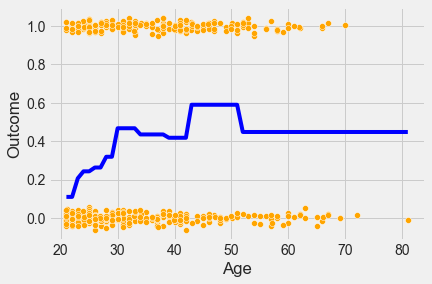
\includegraphics[keepaspectratio]{Logistic Regression_files/figure-pdf/cell-40-output-2.png}}

\bookmarksetup{startatroot}

\chapter{Precision/Recall Tradeoff}\label{precisionrecall-tradeoff}

\begin{Shaded}
\begin{Highlighting}[]
\ImportTok{from}\NormalTok{ sklearn.metrics }\ImportTok{import}\NormalTok{ precision\_recall\_curve}


\KeywordTok{def}\NormalTok{ plot\_precision\_recall\_vs\_threshold(precisions, recalls, thresholds):}
\NormalTok{    plt.plot(thresholds, precisions[:}\OperatorTok{{-}}\DecValTok{1}\NormalTok{], }\StringTok{"b{-}{-}"}\NormalTok{, label}\OperatorTok{=}\StringTok{"Precision"}\NormalTok{)}
\NormalTok{    plt.plot(thresholds, recalls[:}\OperatorTok{{-}}\DecValTok{1}\NormalTok{], }\StringTok{"g{-}{-}"}\NormalTok{, label}\OperatorTok{=}\StringTok{"Recall"}\NormalTok{)}
\NormalTok{    plt.xlabel(}\StringTok{"Threshold"}\NormalTok{)}
\NormalTok{    plt.legend(loc}\OperatorTok{=}\StringTok{"upper left"}\NormalTok{)}
\NormalTok{    plt.title(}\StringTok{"Precisions/recalls tradeoff"}\NormalTok{)}

    
\NormalTok{precisions, recalls, thresholds }\OperatorTok{=}\NormalTok{ precision\_recall\_curve(y\_test, y\_pred\_test)}


\NormalTok{plt.figure(figsize}\OperatorTok{=}\NormalTok{(}\DecValTok{15}\NormalTok{, }\DecValTok{10}\NormalTok{))}
\NormalTok{plt.subplot(}\DecValTok{2}\NormalTok{, }\DecValTok{2}\NormalTok{, }\DecValTok{1}\NormalTok{)}
\NormalTok{plot\_precision\_recall\_vs\_threshold(precisions, recalls, thresholds)}

\NormalTok{plt.subplot(}\DecValTok{2}\NormalTok{, }\DecValTok{2}\NormalTok{, }\DecValTok{2}\NormalTok{)}
\NormalTok{plt.plot(precisions, recalls)}
\NormalTok{plt.xlabel(}\StringTok{"Precision"}\NormalTok{)}
\NormalTok{plt.ylabel(}\StringTok{"Recall"}\NormalTok{)}
\NormalTok{plt.title(}\StringTok{"PR Curve: precisions/recalls tradeoff"}\NormalTok{)}\OperatorTok{;}
\end{Highlighting}
\end{Shaded}

\pandocbounded{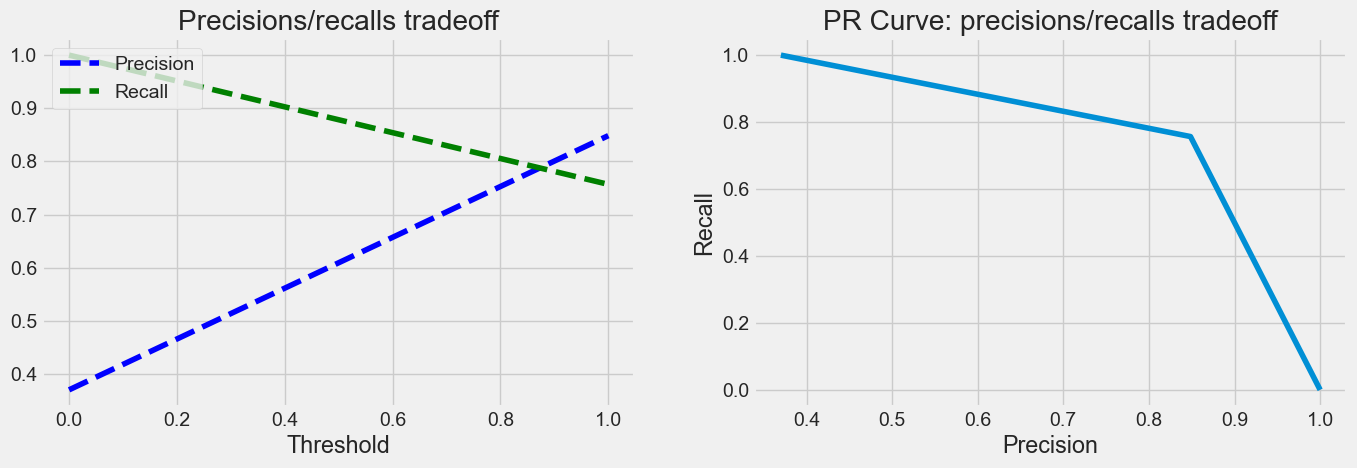
\includegraphics[keepaspectratio]{Logistic Regression_files/figure-pdf/cell-41-output-1.png}}

\section{The Receiver Operating Characteristics (ROC)
Curve}\label{the-receiver-operating-characteristics-roc-curve-1}

A \textbf{ROC(Receiver Operator Characteristic Curve)} is a plot of
sensitivity (True Positive Rate) on the y axis against (1−specificity)
(False Positive Rate) on the x axis for varying values of the threshold
t. The 45° diagonal line connecting (0,0) to (1,1) is the ROC curve
corresponding to random chance. The ROC curve for the gold standard is
the line connecting (0,0) to (0,1) and (0,1) to (1,1).

\pandocbounded{\includegraphics[keepaspectratio]{index_files/mediabag/1-Y65IEOXvxLRKKqWxlQ.png}}

An animation to demonstrate how an ROC curve relates to sensitivity and
specificity for all possible cutoffs.

\begin{figure}[H]

{\centering \pandocbounded{\includegraphics[keepaspectratio]{index_files/mediabag/ROC.gif}}

}

\caption{Alt Text}

\end{figure}%

\href{https://github.com/dariyasydykova/open_projects/blob/master/ROC_animation/animations/ROC.gif}{Source}

\textbf{High Threshold:} * High specificity * Low sensitivity

\textbf{Low Threshold} * Low specificity * High sensitivity

The area under ROC is called \emph{Area Under the Curve(AUC)}. AUC gives
the rate of successful classification by the logistic model. To get a
more in-depth idea of what a ROC-AUC curve is and how is it calculated,
here is a
\href{https://www.analyticsvidhya.com/blog/2020/06/auc-roc-curve-machine-learning/}{link}

\begin{Shaded}
\begin{Highlighting}[]
\ImportTok{from}\NormalTok{ sklearn.metrics }\ImportTok{import}\NormalTok{ roc\_curve}


\KeywordTok{def}\NormalTok{ plot\_roc\_curve(fpr, tpr, label}\OperatorTok{=}\VariableTok{None}\NormalTok{):}
\NormalTok{    plt.plot(fpr, tpr, linewidth}\OperatorTok{=}\DecValTok{2}\NormalTok{, label}\OperatorTok{=}\NormalTok{label)}
\NormalTok{    plt.plot([}\DecValTok{0}\NormalTok{, }\DecValTok{1}\NormalTok{], [}\DecValTok{0}\NormalTok{, }\DecValTok{1}\NormalTok{], }\StringTok{"k{-}{-}"}\NormalTok{)}
\NormalTok{    plt.axis([}\DecValTok{0}\NormalTok{, }\DecValTok{1}\NormalTok{, }\DecValTok{0}\NormalTok{, }\DecValTok{1}\NormalTok{])}
\NormalTok{    plt.xlabel(}\StringTok{\textquotesingle{}False Positive Rate\textquotesingle{}}\NormalTok{)}
\NormalTok{    plt.ylabel(}\StringTok{\textquotesingle{}True Positive Rate\textquotesingle{}}\NormalTok{)}
\NormalTok{    plt.title(}\StringTok{\textquotesingle{}ROC Curve\textquotesingle{}}\NormalTok{)}

\NormalTok{fpr, tpr, thresholds }\OperatorTok{=}\NormalTok{ roc\_curve(y\_test, y\_pred\_test)}
\NormalTok{plt.figure(figsize}\OperatorTok{=}\NormalTok{(}\DecValTok{9}\NormalTok{,}\DecValTok{6}\NormalTok{))}\OperatorTok{;} 
\NormalTok{plot\_roc\_curve(fpr, tpr)}
\NormalTok{plt.show()}\OperatorTok{;}
\end{Highlighting}
\end{Shaded}

\pandocbounded{\includegraphics[keepaspectratio]{Logistic Regression_files/figure-pdf/cell-42-output-1.png}}

\begin{Shaded}
\begin{Highlighting}[]
\ImportTok{from}\NormalTok{ sklearn.metrics }\ImportTok{import}\NormalTok{ roc\_auc\_score}

\NormalTok{roc\_auc\_score(y\_test, y\_pred\_test)}
\end{Highlighting}
\end{Shaded}

\begin{verbatim}
0.8386958386958387
\end{verbatim}

\bookmarksetup{startatroot}

\chapter{Logistic regression: Others}\label{logistic-regression-others}

\begin{Shaded}
\begin{Highlighting}[]
\CommentTok{\# Importing libraries}
\ImportTok{import}\NormalTok{ numpy }\ImportTok{as}\NormalTok{ np}
\ImportTok{import}\NormalTok{ pandas }\ImportTok{as}\NormalTok{ pd}
\ImportTok{import}\NormalTok{ matplotlib.pyplot }\ImportTok{as}\NormalTok{ plt}
\ImportTok{import}\NormalTok{ seaborn }\ImportTok{as}\NormalTok{ sns}
\ImportTok{from}\NormalTok{ sklearn.preprocessing }\ImportTok{import}\NormalTok{ LabelEncoder}
\ImportTok{from}\NormalTok{ sklearn.linear\_model }\ImportTok{import}\NormalTok{ LogisticRegression}
\ImportTok{from}\NormalTok{ sklearn.metrics }\ImportTok{import}\NormalTok{ accuracy\_score, confusion\_matrix}

\NormalTok{sns.}\BuiltInTok{set}\NormalTok{()}
\end{Highlighting}
\end{Shaded}

\section{Decision Boundary in
Classification}\label{decision-boundary-in-classification}

\begin{Shaded}
\begin{Highlighting}[]
\CommentTok{\# Importing the dataset}
\NormalTok{dataset }\OperatorTok{=}\NormalTok{ pd.read\_csv(}\StringTok{\textquotesingle{}datasets/apples\_and\_oranges.csv\textquotesingle{}}\NormalTok{)}
\NormalTok{dataset.head()}
\end{Highlighting}
\end{Shaded}

\begin{longtable}[]{@{}llll@{}}
\toprule\noalign{}
& Weight & Size & Class \\
\midrule\noalign{}
\endhead
\bottomrule\noalign{}
\endlastfoot
0 & 69 & 4.39 & orange \\
1 & 69 & 4.21 & orange \\
2 & 65 & 4.09 & orange \\
3 & 72 & 5.85 & apple \\
4 & 67 & 4.70 & orange \\
\end{longtable}

\begin{Shaded}
\begin{Highlighting}[]
\CommentTok{\# No. of apples and oranges}
\NormalTok{dataset[}\StringTok{\textquotesingle{}Class\textquotesingle{}}\NormalTok{].value\_counts()}
\end{Highlighting}
\end{Shaded}

\begin{verbatim}
Class
orange    20
apple     20
Name: count, dtype: int64
\end{verbatim}

\subsection{Encoding Target}\label{encoding-target}

\begin{Shaded}
\begin{Highlighting}[]
\NormalTok{le }\OperatorTok{=}\NormalTok{ LabelEncoder()}
\NormalTok{dataset[}\StringTok{\textquotesingle{}Class\textquotesingle{}}\NormalTok{] }\OperatorTok{=}\NormalTok{ le.fit\_transform(dataset[}\StringTok{\textquotesingle{}Class\textquotesingle{}}\NormalTok{])}
\NormalTok{le.classes\_}
\end{Highlighting}
\end{Shaded}

\begin{verbatim}
array(['apple', 'orange'], dtype=object)
\end{verbatim}

This implies that, * 0 represents Apple * 1 represents Orange

\begin{Shaded}
\begin{Highlighting}[]
\NormalTok{dataset.head()}
\end{Highlighting}
\end{Shaded}

\begin{longtable}[]{@{}llll@{}}
\toprule\noalign{}
& Weight & Size & Class \\
\midrule\noalign{}
\endhead
\bottomrule\noalign{}
\endlastfoot
0 & 69 & 4.39 & 1 \\
1 & 69 & 4.21 & 1 \\
2 & 65 & 4.09 & 1 \\
3 & 72 & 5.85 & 0 \\
4 & 67 & 4.70 & 1 \\
\end{longtable}

\subsection{Plotting the dataset}\label{plotting-the-dataset}

\begin{Shaded}
\begin{Highlighting}[]
\NormalTok{plt.figure(figsize}\OperatorTok{=}\NormalTok{(}\DecValTok{9}\NormalTok{,}\DecValTok{6}\NormalTok{))}
\NormalTok{plt.title(}\StringTok{\textquotesingle{}Apples and Oranges\textquotesingle{}}\NormalTok{, fontweight}\OperatorTok{=}\StringTok{\textquotesingle{}bold\textquotesingle{}}\NormalTok{, fontsize}\OperatorTok{=}\DecValTok{16}\NormalTok{)}
\NormalTok{plt.xlabel(}\StringTok{\textquotesingle{}Weight\textquotesingle{}}\NormalTok{)}
\NormalTok{plt.ylabel(}\StringTok{\textquotesingle{}Size\textquotesingle{}}\NormalTok{)}
\NormalTok{scatter }\OperatorTok{=}\NormalTok{ plt.scatter(dataset[}\StringTok{\textquotesingle{}Weight\textquotesingle{}}\NormalTok{], dataset[}\StringTok{\textquotesingle{}Size\textquotesingle{}}\NormalTok{], c}\OperatorTok{=}\NormalTok{dataset[}\StringTok{\textquotesingle{}Class\textquotesingle{}}\NormalTok{], cmap}\OperatorTok{=}\StringTok{\textquotesingle{}viridis\textquotesingle{}}\NormalTok{)}
\NormalTok{plt.legend(}\OperatorTok{*}\NormalTok{scatter.legend\_elements(),}
\NormalTok{           loc }\OperatorTok{=} \StringTok{\textquotesingle{}upper left\textquotesingle{}}\NormalTok{,}
\NormalTok{           title }\OperatorTok{=} \StringTok{\textquotesingle{}Class\textquotesingle{}}\NormalTok{)}\OperatorTok{;}
\end{Highlighting}
\end{Shaded}

\pandocbounded{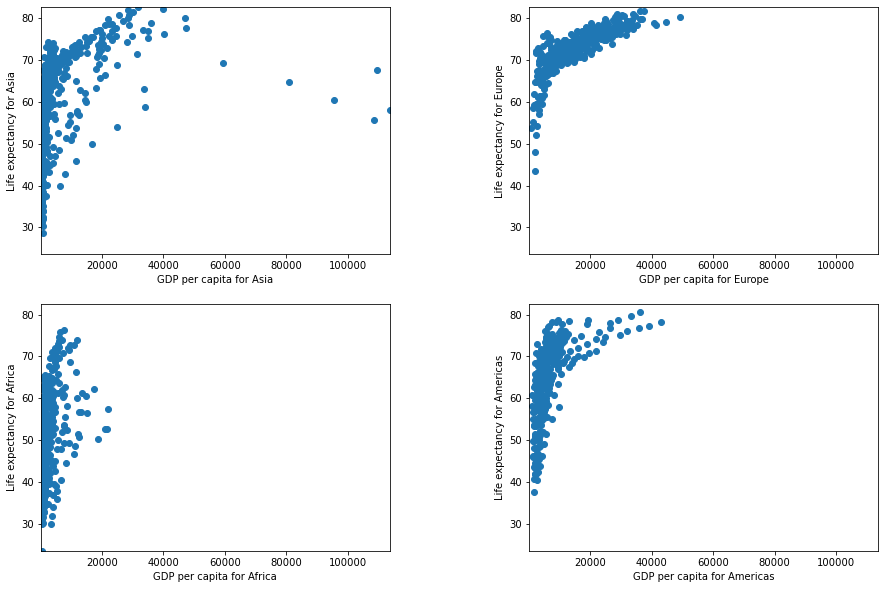
\includegraphics[keepaspectratio]{Logistic Regression - Decision Boundary and Feature Engineering (Nonlinear Features)_files/figure-pdf/cell-7-output-1.png}}

We can observe that oranges have lower weight and size compared to
apples. Further by drawing a straight line between these two groups of
data points, we can clearly distinguish between apples and oranges.

\subsection{Building a Logistic Regression model to distinguish apples
and
oranges}\label{building-a-logistic-regression-model-to-distinguish-apples-and-oranges}

As we can clearly distinguish between apples and oranges using a
straight line decision boundary, we can choose the hypothesis \emph{y =
a0 + a1 } x1 + a2 * x2* for Logistic Regression where, \emph{a0},
\emph{a1}, \emph{a2} are the fitting parameters \emph{x1} is Weight
\emph{x2} is Size

\begin{Shaded}
\begin{Highlighting}[]
\CommentTok{\# Defining target and features}
\NormalTok{y }\OperatorTok{=}\NormalTok{ dataset[}\StringTok{\textquotesingle{}Class\textquotesingle{}}\NormalTok{]}
\NormalTok{x }\OperatorTok{=}\NormalTok{ dataset.drop(columns}\OperatorTok{=}\NormalTok{[}\StringTok{\textquotesingle{}Class\textquotesingle{}}\NormalTok{])}
\end{Highlighting}
\end{Shaded}

\begin{Shaded}
\begin{Highlighting}[]
\CommentTok{\# Creating object of LogisticRegression class}
\NormalTok{log\_reg }\OperatorTok{=}\NormalTok{ LogisticRegression()}
\end{Highlighting}
\end{Shaded}

\begin{Shaded}
\begin{Highlighting}[]
\CommentTok{\# Fitting parameters}
\NormalTok{log\_reg.fit(x,y)}
\end{Highlighting}
\end{Shaded}

\begin{verbatim}
LogisticRegression()
\end{verbatim}

\begin{Shaded}
\begin{Highlighting}[]
\CommentTok{\# Intercept {-} a0}
\NormalTok{log\_reg.intercept\_}
\end{Highlighting}
\end{Shaded}

\begin{verbatim}
array([106.60287324])
\end{verbatim}

\begin{Shaded}
\begin{Highlighting}[]
\CommentTok{\# Coefficients {-} a1, a2 respectively}
\NormalTok{log\_reg.coef\_}
\end{Highlighting}
\end{Shaded}

\begin{verbatim}
array([[-1.42833694, -1.31285258]])
\end{verbatim}

\begin{Shaded}
\begin{Highlighting}[]
\CommentTok{\# Predicting labels for the given dataset}
\NormalTok{label\_predictions }\OperatorTok{=}\NormalTok{ log\_reg.predict(x)}
\NormalTok{label\_predictions}
\end{Highlighting}
\end{Shaded}

\begin{verbatim}
array([1, 1, 1, 0, 1, 0, 0, 0, 0, 1, 0, 0, 0, 1, 0, 1, 1, 0, 1, 0, 1, 1,
       1, 1, 1, 0, 1, 1, 0, 0, 0, 1, 0, 0, 1, 1, 1, 0, 0, 0])
\end{verbatim}

\subsection{Linear Decision Boundary with naive
features}\label{linear-decision-boundary-with-naive-features}

\begin{Shaded}
\begin{Highlighting}[]
\CommentTok{\# Parameter values}
\NormalTok{a0 }\OperatorTok{=}\NormalTok{ log\_reg.intercept\_[}\DecValTok{0}\NormalTok{]}
\NormalTok{a1 }\OperatorTok{=}\NormalTok{ log\_reg.coef\_[}\DecValTok{0}\NormalTok{][}\DecValTok{0}\NormalTok{]}
\NormalTok{a2 }\OperatorTok{=}\NormalTok{ log\_reg.coef\_[}\DecValTok{0}\NormalTok{][}\DecValTok{1}\NormalTok{]}
\end{Highlighting}
\end{Shaded}

\begin{Shaded}
\begin{Highlighting}[]
\CommentTok{\# Defining x1 and x2 values for decision boundary}
\NormalTok{x1 }\OperatorTok{=}\NormalTok{ np.array([}\DecValTok{69}\NormalTok{, }\DecValTok{71}\NormalTok{])}
\NormalTok{x2 }\OperatorTok{=}\NormalTok{ (}\FloatTok{0.5} \OperatorTok{{-}}\NormalTok{a0 }\OperatorTok{{-}}\NormalTok{ (a1 }\OperatorTok{*}\NormalTok{ x1)) }\OperatorTok{/}\NormalTok{ a2}
\end{Highlighting}
\end{Shaded}

\begin{Shaded}
\begin{Highlighting}[]
\CommentTok{\# Plotting the decision boundary}
\NormalTok{plt.figure(figsize}\OperatorTok{=}\NormalTok{(}\DecValTok{9}\NormalTok{,}\DecValTok{6}\NormalTok{))}
\NormalTok{plt.title(}\StringTok{\textquotesingle{}Apples and Oranges\textquotesingle{}}\NormalTok{, fontweight}\OperatorTok{=}\StringTok{\textquotesingle{}bold\textquotesingle{}}\NormalTok{, fontsize}\OperatorTok{=}\DecValTok{16}\NormalTok{)}
\NormalTok{plt.xlabel(}\StringTok{\textquotesingle{}Weight\textquotesingle{}}\NormalTok{)}
\NormalTok{plt.ylabel(}\StringTok{\textquotesingle{}Size\textquotesingle{}}\NormalTok{)}
\NormalTok{scatter }\OperatorTok{=}\NormalTok{ plt.scatter(dataset[}\StringTok{\textquotesingle{}Weight\textquotesingle{}}\NormalTok{], dataset[}\StringTok{\textquotesingle{}Size\textquotesingle{}}\NormalTok{], c}\OperatorTok{=}\NormalTok{dataset[}\StringTok{\textquotesingle{}Class\textquotesingle{}}\NormalTok{], cmap}\OperatorTok{=}\StringTok{\textquotesingle{}viridis\textquotesingle{}}\NormalTok{)}
\NormalTok{plt.legend(}\OperatorTok{*}\NormalTok{scatter.legend\_elements(),}
\NormalTok{           loc }\OperatorTok{=} \StringTok{\textquotesingle{}upper left\textquotesingle{}}\NormalTok{,}
\NormalTok{           title }\OperatorTok{=} \StringTok{\textquotesingle{}Class\textquotesingle{}}\NormalTok{)}
\NormalTok{plt.plot(x1, x2, color}\OperatorTok{=}\StringTok{\textquotesingle{}red\textquotesingle{}}\NormalTok{, label}\OperatorTok{=}\StringTok{\textquotesingle{}Decision Boundary\textquotesingle{}}\NormalTok{)}
\NormalTok{plt.show()}
\end{Highlighting}
\end{Shaded}

\pandocbounded{\includegraphics[keepaspectratio]{Logistic Regression - Decision Boundary and Feature Engineering (Nonlinear Features)_files/figure-pdf/cell-16-output-1.png}}

In this problem, we have just two features x1 and x2, if we use just
those as they are we will end up with a straight line which divides our
2D plane into two half-planes.

\section{Non-linear Decision
Boundary}\label{non-linear-decision-boundary}

In some occasions, we want to have a more complex boundary, and we can
achieve this by transforming our features, if we have features like this
\[(x_1, x_2, x_1x_2, x_1^2, x_2^2)\] That is adding interaction terms
and polynominal terms (degree = 2), the decision boundary will look like
this
\pandocbounded{\includegraphics[keepaspectratio]{index_files/mediabag/1520148127787-e=1714.pdf}}

For instance, when confronted with a training data distribution as
illustrated below,
\pandocbounded{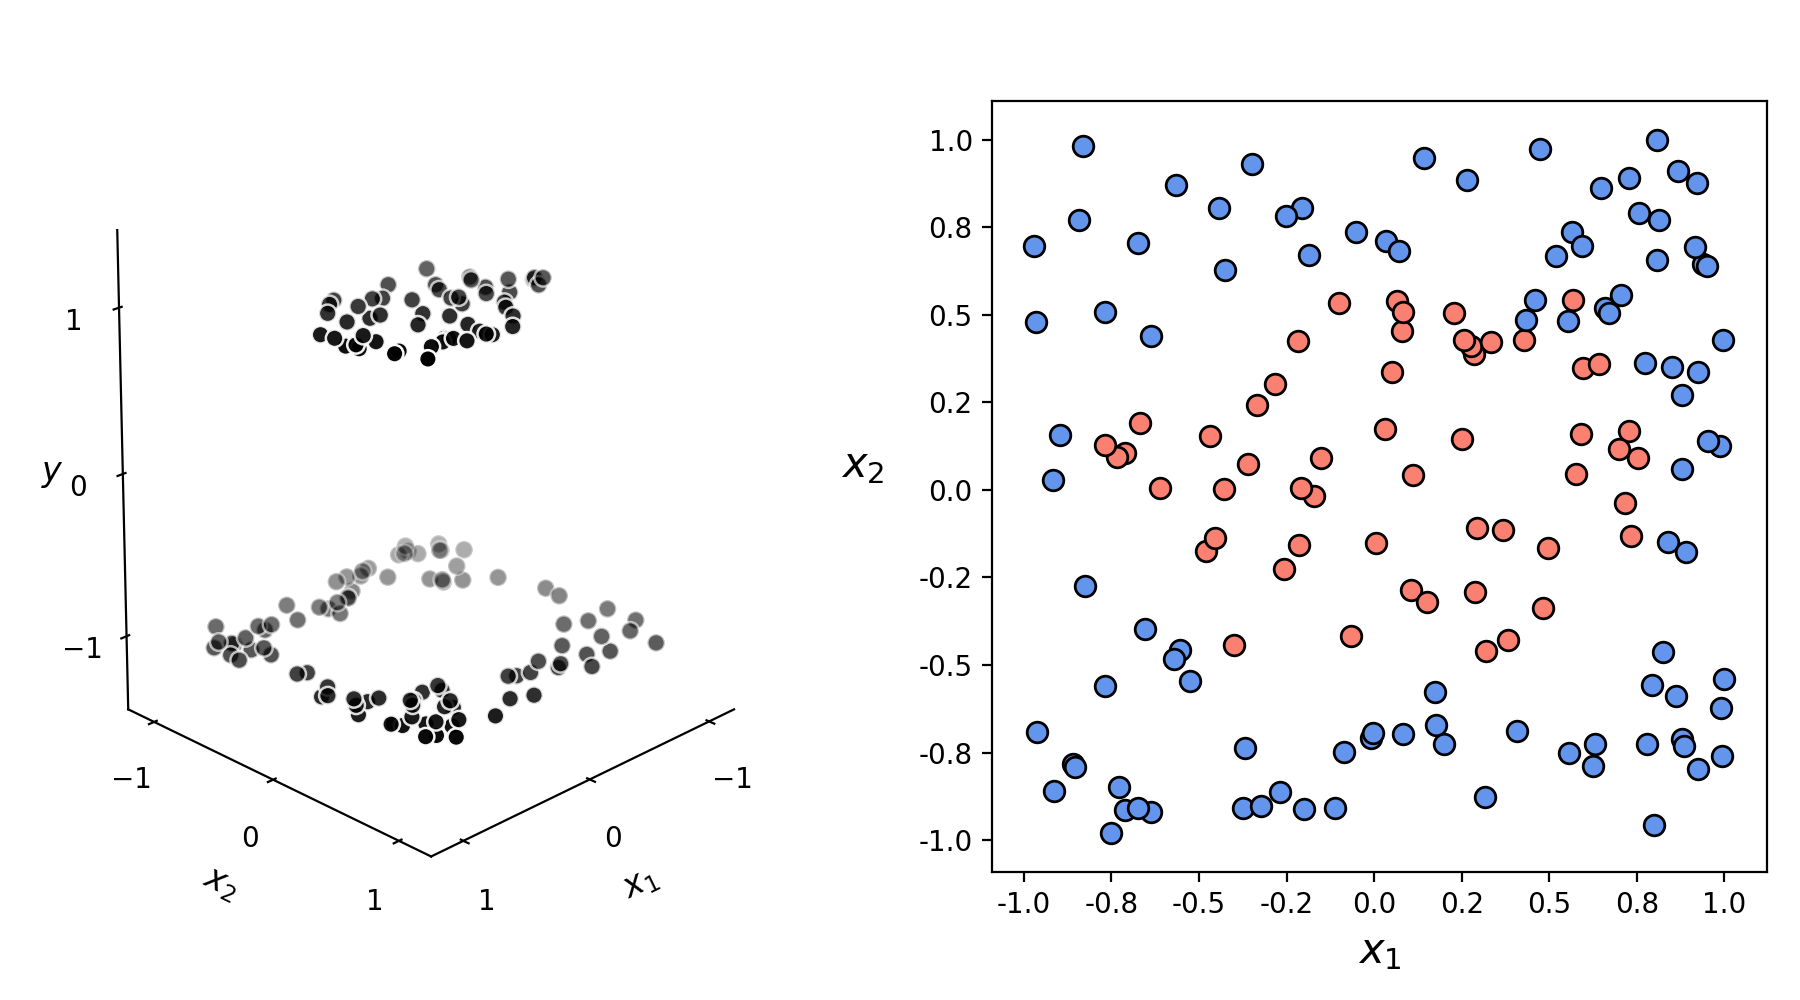
\includegraphics[keepaspectratio]{Logistic Regression - Decision Boundary and Feature Engineering (Nonlinear Features)_files/figure-pdf/68c4db82-1-image-2.png}}
it becomes imperative to generate polynomial features \[(x_1^2, x_2^2)\]
in order to enhance the delineation between the two classes.
\pandocbounded{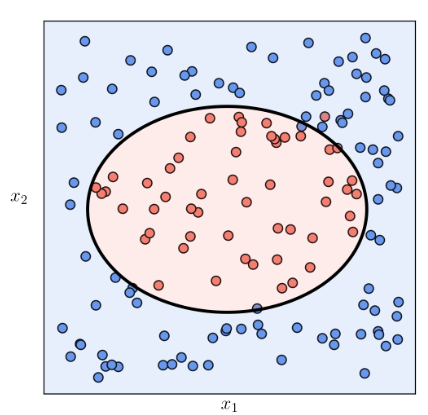
\includegraphics[keepaspectratio]{Logistic Regression - Decision Boundary and Feature Engineering (Nonlinear Features)_files/figure-pdf/68c4db82-2-image-3.png}}

Let's delve into a concrete example below to illustrate this concept.For
the purpose of illustrating the decision boundary, I chose not to split
the data into training and test sets.

\begin{Shaded}
\begin{Highlighting}[]
\CommentTok{\#Load our Dataset for Logistic Regression}
\NormalTok{components }\OperatorTok{=}\NormalTok{ pd.read\_csv(}\StringTok{\textquotesingle{}datasets/ex2data2.txt\textquotesingle{}}\NormalTok{, header}\OperatorTok{=}\VariableTok{None}\NormalTok{, names }\OperatorTok{=}\NormalTok{ [}\StringTok{\textquotesingle{}feature 1\textquotesingle{}}\NormalTok{, }\StringTok{\textquotesingle{}feature 2\textquotesingle{}}\NormalTok{, }\StringTok{\textquotesingle{}faulty\textquotesingle{}}\NormalTok{])}
\NormalTok{components.head()}
\end{Highlighting}
\end{Shaded}

\begin{longtable}[]{@{}llll@{}}
\toprule\noalign{}
& feature 1 & feature 2 & faulty \\
\midrule\noalign{}
\endhead
\bottomrule\noalign{}
\endlastfoot
0 & 0.051267 & 0.69956 & 1 \\
1 & -0.092742 & 0.68494 & 1 \\
2 & -0.213710 & 0.69225 & 1 \\
3 & -0.375000 & 0.50219 & 1 \\
4 & -0.513250 & 0.46564 & 1 \\
\end{longtable}

\begin{Shaded}
\begin{Highlighting}[]
\CommentTok{\# check the balance of the dataset}
\NormalTok{components[}\StringTok{\textquotesingle{}faulty\textquotesingle{}}\NormalTok{].value\_counts()}
\end{Highlighting}
\end{Shaded}

\begin{verbatim}
faulty
0    60
1    58
Name: count, dtype: int64
\end{verbatim}

\begin{Shaded}
\begin{Highlighting}[]
\CommentTok{\# get positive and negative samples for plotting}
\NormalTok{pos }\OperatorTok{=}\NormalTok{ components[}\StringTok{\textquotesingle{}faulty\textquotesingle{}}\NormalTok{] }\OperatorTok{==} \DecValTok{1}
\NormalTok{neg }\OperatorTok{=}\NormalTok{ components[}\StringTok{\textquotesingle{}faulty\textquotesingle{}}\NormalTok{] }\OperatorTok{==} \DecValTok{0}
\end{Highlighting}
\end{Shaded}

\begin{Shaded}
\begin{Highlighting}[]
\CommentTok{\# Visualize Data}
\NormalTok{fig, axes }\OperatorTok{=}\NormalTok{ plt.subplots()}\OperatorTok{;}
\NormalTok{axes.set\_xlabel(}\StringTok{\textquotesingle{}Feature 1\textquotesingle{}}\NormalTok{)}
\NormalTok{axes.set\_ylabel(}\StringTok{\textquotesingle{}Feature 2\textquotesingle{}}\NormalTok{)}
\NormalTok{axes.scatter(components.loc[pos, }\StringTok{\textquotesingle{}feature 1\textquotesingle{}}\NormalTok{], components.loc[pos, }\StringTok{\textquotesingle{}feature 2\textquotesingle{}}\NormalTok{], color }\OperatorTok{=} \StringTok{\textquotesingle{}r\textquotesingle{}}\NormalTok{, marker}\OperatorTok{=}\StringTok{\textquotesingle{}x\textquotesingle{}}\NormalTok{, label}\OperatorTok{=}\StringTok{\textquotesingle{}Faulty\textquotesingle{}}\NormalTok{)}
\NormalTok{axes.scatter(components.loc[neg, }\StringTok{\textquotesingle{}feature 1\textquotesingle{}}\NormalTok{], components.loc[neg, }\StringTok{\textquotesingle{}feature 2\textquotesingle{}}\NormalTok{], color }\OperatorTok{=} \StringTok{\textquotesingle{}g\textquotesingle{}}\NormalTok{, marker}\OperatorTok{=}\StringTok{\textquotesingle{}o\textquotesingle{}}\NormalTok{, label}\OperatorTok{=}\StringTok{\textquotesingle{}Non Faculty\textquotesingle{}}\NormalTok{)}
\NormalTok{axes.legend(title}\OperatorTok{=}\StringTok{\textquotesingle{}Legend\textquotesingle{}}\NormalTok{, loc }\OperatorTok{=} \StringTok{\textquotesingle{}best\textquotesingle{}}\NormalTok{ )}
\NormalTok{axes.set\_xlim(}\OperatorTok{{-}}\DecValTok{1}\NormalTok{,}\FloatTok{1.5}\NormalTok{)}
\NormalTok{axes.set\_xlim(}\OperatorTok{{-}}\DecValTok{1}\NormalTok{,}\FloatTok{1.5}\NormalTok{)}
\end{Highlighting}
\end{Shaded}

\pandocbounded{\includegraphics[keepaspectratio]{Logistic Regression - Decision Boundary and Feature Engineering (Nonlinear Features)_files/figure-pdf/cell-20-output-1.png}}

As we can see that the positive and negative examples are not linearly
seperable. So we have to add additional higher order polynomial
features.

\begin{Shaded}
\begin{Highlighting}[]
\CommentTok{\# define function to map higher order polynomial features}
\KeywordTok{def}\NormalTok{ mapFeature(X1, X2, degree):}
\NormalTok{    res }\OperatorTok{=}\NormalTok{ np.ones(X1.shape[}\DecValTok{0}\NormalTok{])}
    \ControlFlowTok{for}\NormalTok{ i }\KeywordTok{in} \BuiltInTok{range}\NormalTok{(}\DecValTok{1}\NormalTok{,degree }\OperatorTok{+} \DecValTok{1}\NormalTok{):}
        \ControlFlowTok{for}\NormalTok{ j }\KeywordTok{in} \BuiltInTok{range}\NormalTok{(}\DecValTok{0}\NormalTok{,i }\OperatorTok{+} \DecValTok{1}\NormalTok{):}
\NormalTok{            res }\OperatorTok{=}\NormalTok{ np.column\_stack((res, (X1 }\OperatorTok{**}\NormalTok{ (i}\OperatorTok{{-}}\NormalTok{j)) }\OperatorTok{*}\NormalTok{ (X2 }\OperatorTok{**}\NormalTok{ j)))}
    
    \ControlFlowTok{return}\NormalTok{ res}
\end{Highlighting}
\end{Shaded}

\begin{Shaded}
\begin{Highlighting}[]
\CommentTok{\# Get the features }
\NormalTok{X }\OperatorTok{=}\NormalTok{ components.iloc[:, :}\DecValTok{2}\NormalTok{]}
\end{Highlighting}
\end{Shaded}

\begin{Shaded}
\begin{Highlighting}[]
\NormalTok{degree }\OperatorTok{=} \DecValTok{2}
\end{Highlighting}
\end{Shaded}

\begin{Shaded}
\begin{Highlighting}[]
\NormalTok{X\_poly }\OperatorTok{=}\NormalTok{ mapFeature(X.iloc[:, }\DecValTok{0}\NormalTok{], X.iloc[:, }\DecValTok{1}\NormalTok{], degree)}
\end{Highlighting}
\end{Shaded}

\begin{Shaded}
\begin{Highlighting}[]
\CommentTok{\# Get the target variable}
\NormalTok{y }\OperatorTok{=}\NormalTok{ components.iloc[:, }\DecValTok{2}\NormalTok{]}
\end{Highlighting}
\end{Shaded}

\begin{Shaded}
\begin{Highlighting}[]
\KeywordTok{def}\NormalTok{ sigmoid(z):}
    \ControlFlowTok{return} \DecValTok{1} \OperatorTok{/}\NormalTok{ (}\DecValTok{1} \OperatorTok{+}\NormalTok{ np.exp(}\OperatorTok{{-}}\NormalTok{z))}
\end{Highlighting}
\end{Shaded}

\begin{Shaded}
\begin{Highlighting}[]
\KeywordTok{def}\NormalTok{ costFunc(theta, X, y):}
\NormalTok{    m }\OperatorTok{=}\NormalTok{ y.shape[}\DecValTok{0}\NormalTok{]}
\NormalTok{    z }\OperatorTok{=}\NormalTok{ X.dot(theta)}
\NormalTok{    h }\OperatorTok{=}\NormalTok{ sigmoid(z)}
\NormalTok{    term1 }\OperatorTok{=}\NormalTok{ y }\OperatorTok{*}\NormalTok{ np.log(h)}
\NormalTok{    term2 }\OperatorTok{=}\NormalTok{ (}\DecValTok{1}\OperatorTok{{-}}\NormalTok{ y) }\OperatorTok{*}\NormalTok{ np.log(}\DecValTok{1} \OperatorTok{{-}}\NormalTok{ h)}
\NormalTok{    J }\OperatorTok{=} \OperatorTok{{-}}\NormalTok{np.}\BuiltInTok{sum}\NormalTok{(term1 }\OperatorTok{+}\NormalTok{ term2, axis }\OperatorTok{=} \DecValTok{0}\NormalTok{) }\OperatorTok{/}\NormalTok{ m}
    \ControlFlowTok{return}\NormalTok{ J }
\end{Highlighting}
\end{Shaded}

\begin{Shaded}
\begin{Highlighting}[]
\CommentTok{\# Set initial values for our parameters}
\NormalTok{initial\_theta }\OperatorTok{=}\NormalTok{ np.zeros(X\_poly.shape[}\DecValTok{1}\NormalTok{]).reshape(X\_poly.shape[}\DecValTok{1}\NormalTok{], }\DecValTok{1}\NormalTok{)}
\end{Highlighting}
\end{Shaded}

\begin{Shaded}
\begin{Highlighting}[]
\CommentTok{\# Now call the optimization routine}
\CommentTok{\#NOTE: This automatically picks the learning rate}
\ImportTok{from}\NormalTok{ scipy.optimize }\ImportTok{import}\NormalTok{ minimize}
\NormalTok{res }\OperatorTok{=}\NormalTok{ minimize(costFunc, initial\_theta.flatten(), args}\OperatorTok{=}\NormalTok{(X\_poly, y))}
\end{Highlighting}
\end{Shaded}

\begin{Shaded}
\begin{Highlighting}[]
\CommentTok{\# our optimizated coefficients}
\NormalTok{theta }\OperatorTok{=}\NormalTok{ res.x}
\end{Highlighting}
\end{Shaded}

\begin{Shaded}
\begin{Highlighting}[]
\CommentTok{\# define a function to plot the decision boundary}
\KeywordTok{def}\NormalTok{ plotDecisionBoundary(theta,degree, axes):}
\NormalTok{    u }\OperatorTok{=}\NormalTok{ np.linspace(}\OperatorTok{{-}}\DecValTok{1}\NormalTok{, }\FloatTok{1.5}\NormalTok{, }\DecValTok{50}\NormalTok{)}
\NormalTok{    v }\OperatorTok{=}\NormalTok{ np.linspace(}\OperatorTok{{-}}\DecValTok{1}\NormalTok{, }\FloatTok{1.5}\NormalTok{, }\DecValTok{50}\NormalTok{)}
\NormalTok{    U,V }\OperatorTok{=}\NormalTok{ np.meshgrid(u,v)}
    \CommentTok{\# convert U, V to vectors for calculating additional features}
    \CommentTok{\# using vectorized implementation}
\NormalTok{    U }\OperatorTok{=}\NormalTok{ np.ravel(U)}
\NormalTok{    V }\OperatorTok{=}\NormalTok{ np.ravel(V)}
\NormalTok{    Z }\OperatorTok{=}\NormalTok{ np.zeros((}\BuiltInTok{len}\NormalTok{(u) }\OperatorTok{*} \BuiltInTok{len}\NormalTok{(v)))}
    
\NormalTok{    X\_poly }\OperatorTok{=}\NormalTok{ mapFeature(U, V, degree)}
\NormalTok{    Z }\OperatorTok{=}\NormalTok{ X\_poly.dot(theta)}
    
    \CommentTok{\# reshape U, V, Z back to matrix}
\NormalTok{    U }\OperatorTok{=}\NormalTok{ U.reshape((}\BuiltInTok{len}\NormalTok{(u), }\BuiltInTok{len}\NormalTok{(v)))}
\NormalTok{    V }\OperatorTok{=}\NormalTok{ V.reshape((}\BuiltInTok{len}\NormalTok{(u), }\BuiltInTok{len}\NormalTok{(v)))}
\NormalTok{    Z }\OperatorTok{=}\NormalTok{ Z.reshape((}\BuiltInTok{len}\NormalTok{(u), }\BuiltInTok{len}\NormalTok{(v)))}
    
\NormalTok{    cs }\OperatorTok{=}\NormalTok{ axes.contour(U,V,Z,levels}\OperatorTok{=}\NormalTok{[}\DecValTok{0}\NormalTok{],cmap}\OperatorTok{=} \StringTok{"Greys\_r"}\NormalTok{)}
\NormalTok{    axes.legend(labels}\OperatorTok{=}\NormalTok{[}\StringTok{\textquotesingle{}Non Faculty\textquotesingle{}}\NormalTok{, }\StringTok{\textquotesingle{}faulty\textquotesingle{}}\NormalTok{, }\StringTok{\textquotesingle{}Decision Boundary\textquotesingle{}}\NormalTok{])}
    \ControlFlowTok{return}\NormalTok{ cs}
\end{Highlighting}
\end{Shaded}

\begin{Shaded}
\begin{Highlighting}[]
\CommentTok{\# Plot Decision boundary}
\NormalTok{fig, axes }\OperatorTok{=}\NormalTok{ plt.subplots()}\OperatorTok{;}
\NormalTok{axes.set\_xlabel(}\StringTok{\textquotesingle{}Feature 1\textquotesingle{}}\NormalTok{)}
\NormalTok{axes.set\_ylabel(}\StringTok{\textquotesingle{}Feature 2\textquotesingle{}}\NormalTok{)}
\NormalTok{axes.scatter(components.loc[pos, }\StringTok{\textquotesingle{}feature 1\textquotesingle{}}\NormalTok{], components.loc[pos, }\StringTok{\textquotesingle{}feature 2\textquotesingle{}}\NormalTok{], color }\OperatorTok{=} \StringTok{\textquotesingle{}r\textquotesingle{}}\NormalTok{, marker}\OperatorTok{=}\StringTok{\textquotesingle{}x\textquotesingle{}}\NormalTok{, label}\OperatorTok{=}\StringTok{\textquotesingle{}Faulty\textquotesingle{}}\NormalTok{)}
\NormalTok{axes.scatter(components.loc[neg, }\StringTok{\textquotesingle{}feature 1\textquotesingle{}}\NormalTok{], components.loc[neg, }\StringTok{\textquotesingle{}feature 2\textquotesingle{}}\NormalTok{], color }\OperatorTok{=} \StringTok{\textquotesingle{}g\textquotesingle{}}\NormalTok{, marker}\OperatorTok{=}\StringTok{\textquotesingle{}o\textquotesingle{}}\NormalTok{, label}\OperatorTok{=}\StringTok{\textquotesingle{}Good\textquotesingle{}}\NormalTok{)}
\CommentTok{\#axes.legend(title=\textquotesingle{}Legend\textquotesingle{}, loc = \textquotesingle{}best\textquotesingle{} )}

\NormalTok{plotDecisionBoundary(theta, degree, axes)}\OperatorTok{;}
\end{Highlighting}
\end{Shaded}

\pandocbounded{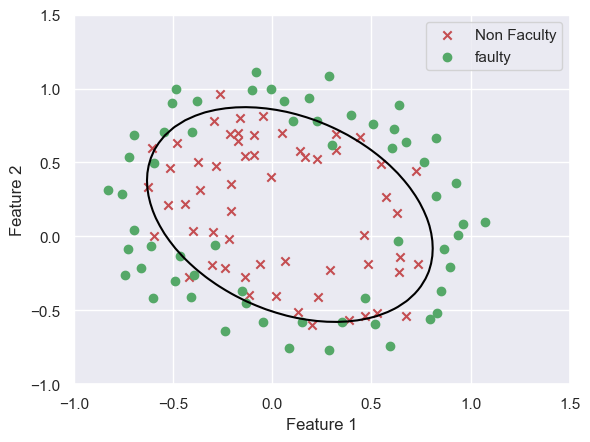
\includegraphics[keepaspectratio]{Logistic Regression - Decision Boundary and Feature Engineering (Nonlinear Features)_files/figure-pdf/cell-32-output-1.png}}

of course, you can increase the degree of the polynomial you want to
fit, but the overfitting could become a problem

\begin{Shaded}
\begin{Highlighting}[]
\CommentTok{\# set degree = 6}
\NormalTok{degree }\OperatorTok{=} \DecValTok{6}
\CommentTok{\# map features to the degree}
\NormalTok{X\_poly }\OperatorTok{=}\NormalTok{ mapFeature(X.iloc[:, }\DecValTok{0}\NormalTok{], X.iloc[:, }\DecValTok{1}\NormalTok{], degree)}
\CommentTok{\# set initial parameters}
\NormalTok{initial\_theta }\OperatorTok{=}\NormalTok{ np.zeros(X\_poly.shape[}\DecValTok{1}\NormalTok{]).reshape(X\_poly.shape[}\DecValTok{1}\NormalTok{], }\DecValTok{1}\NormalTok{)}
\end{Highlighting}
\end{Shaded}

\begin{Shaded}
\begin{Highlighting}[]
\CommentTok{\# Run the optimization function}
\NormalTok{res }\OperatorTok{=}\NormalTok{ minimize(costFunc, initial\_theta.flatten(), args}\OperatorTok{=}\NormalTok{(X\_poly, y))}
\NormalTok{theta }\OperatorTok{=}\NormalTok{ res.x.reshape(res.x.shape[}\DecValTok{0}\NormalTok{], }\DecValTok{1}\NormalTok{)}

\CommentTok{\# Plot Decision boundary}
\NormalTok{fig, axes }\OperatorTok{=}\NormalTok{ plt.subplots()}
\NormalTok{axes.set\_xlabel(}\StringTok{\textquotesingle{}Feature 1\textquotesingle{}}\NormalTok{)}
\NormalTok{axes.set\_ylabel(}\StringTok{\textquotesingle{}Feature 2\textquotesingle{}}\NormalTok{)}
\NormalTok{axes.scatter(components.loc[pos, }\StringTok{\textquotesingle{}feature 1\textquotesingle{}}\NormalTok{], components.loc[pos, }\StringTok{\textquotesingle{}feature 2\textquotesingle{}}\NormalTok{], color}\OperatorTok{=}\StringTok{\textquotesingle{}r\textquotesingle{}}\NormalTok{, marker}\OperatorTok{=}\StringTok{\textquotesingle{}x\textquotesingle{}}\NormalTok{, label}\OperatorTok{=}\StringTok{\textquotesingle{}Faulty\textquotesingle{}}\NormalTok{)}
\NormalTok{axes.scatter(components.loc[neg, }\StringTok{\textquotesingle{}feature 1\textquotesingle{}}\NormalTok{], components.loc[neg, }\StringTok{\textquotesingle{}feature 2\textquotesingle{}}\NormalTok{], color}\OperatorTok{=}\StringTok{\textquotesingle{}g\textquotesingle{}}\NormalTok{, marker}\OperatorTok{=}\StringTok{\textquotesingle{}o\textquotesingle{}}\NormalTok{, label}\OperatorTok{=}\StringTok{\textquotesingle{}Good\textquotesingle{}}\NormalTok{)}
\CommentTok{\#axes.legend(title=\textquotesingle{}Legend\textquotesingle{}, loc=\textquotesingle{}best\textquotesingle{})}

\NormalTok{plotDecisionBoundary(theta, degree, axes)}
\end{Highlighting}
\end{Shaded}

\pandocbounded{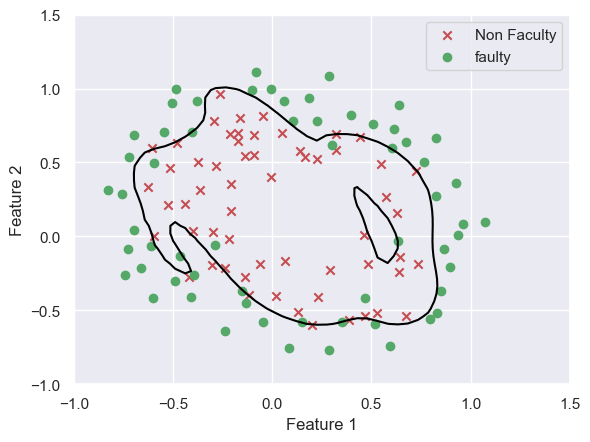
\includegraphics[keepaspectratio]{Logistic Regression - Decision Boundary and Feature Engineering (Nonlinear Features)_files/figure-pdf/cell-34-output-1.png}}

As we can see the model tries pretty hard to capture every single
example perfectly and overfits the data. This kind of model has
overfitting issue. i.e The model has not pre-conceived notion about the
seperation of the positive and negative examples and pretty much can fit
any kind of data. Such model will fail in predicting the correct
classification when it sees new examples.

One of techiques is to use regularization, which we will cover later.
The idea is to penalize the algorithm when it tries to overfit by adding
a regularization term to the cost function.

The New Cost function with the regularization is specified as

\(J(\theta ) = \frac{1}{m} \sum_{i=1}^m[-y_i log(h_\theta (z_i) – (1 – y_i) log(1-h_\theta (z_i))] +
                    \frac{\lambda}{2m} \sum_{j=1}^n[\theta_j^2]\)

where \(\lambda\) = regularization factor n = number of features. (NOTE:
The regularization term does include the intercept term \(\theta_0\)

\subsection{By adding Polynomial
Features}\label{by-adding-polynomial-features}

\begin{Shaded}
\begin{Highlighting}[]
\NormalTok{components}
\end{Highlighting}
\end{Shaded}

\begin{longtable}[]{@{}llll@{}}
\toprule\noalign{}
& feature 1 & feature 2 & faulty \\
\midrule\noalign{}
\endhead
\bottomrule\noalign{}
\endlastfoot
0 & 0.051267 & 0.699560 & 1 \\
1 & -0.092742 & 0.684940 & 1 \\
2 & -0.213710 & 0.692250 & 1 \\
3 & -0.375000 & 0.502190 & 1 \\
4 & -0.513250 & 0.465640 & 1 \\
... & ... & ... & ... \\
113 & -0.720620 & 0.538740 & 0 \\
114 & -0.593890 & 0.494880 & 0 \\
115 & -0.484450 & 0.999270 & 0 \\
116 & -0.006336 & 0.999270 & 0 \\
117 & 0.632650 & -0.030612 & 0 \\
\end{longtable}

\begin{Shaded}
\begin{Highlighting}[]
\NormalTok{X }\OperatorTok{=}\NormalTok{ components[[}\StringTok{\textquotesingle{}feature 1\textquotesingle{}}\NormalTok{, }\StringTok{\textquotesingle{}feature 2\textquotesingle{}}\NormalTok{]]}
\NormalTok{y }\OperatorTok{=}\NormalTok{ components[}\StringTok{\textquotesingle{}faulty\textquotesingle{}}\NormalTok{]}
\end{Highlighting}
\end{Shaded}

\begin{Shaded}
\begin{Highlighting}[]
\ImportTok{from}\NormalTok{ sklearn.preprocessing }\ImportTok{import}\NormalTok{ PolynomialFeatures}
\NormalTok{poly }\OperatorTok{=}\NormalTok{ PolynomialFeatures(degree}\OperatorTok{=}\DecValTok{2}\NormalTok{)}
\NormalTok{X\_poly }\OperatorTok{=}\NormalTok{ poly.fit\_transform(X)}
\end{Highlighting}
\end{Shaded}

\begin{Shaded}
\begin{Highlighting}[]
\NormalTok{feature\_names }\OperatorTok{=}\NormalTok{ poly.get\_feature\_names\_out()}
\BuiltInTok{print}\NormalTok{(feature\_names)}
\end{Highlighting}
\end{Shaded}

\begin{verbatim}
['1' 'feature 1' 'feature 2' 'feature 1^2' 'feature 1 feature 2'
 'feature 2^2']
\end{verbatim}

\begin{Shaded}
\begin{Highlighting}[]
\ImportTok{from}\NormalTok{ sklearn.linear\_model }\ImportTok{import}\NormalTok{ LogisticRegression}

\NormalTok{model }\OperatorTok{=}\NormalTok{ LogisticRegression()}
\NormalTok{model.fit(X\_poly, y)}
\end{Highlighting}
\end{Shaded}

\begin{verbatim}
LogisticRegression()
\end{verbatim}

\begin{Shaded}
\begin{Highlighting}[]
\NormalTok{label\_predictions }\OperatorTok{=}\NormalTok{ model.predict(X\_poly)}
\end{Highlighting}
\end{Shaded}

\subsubsection{Accuracy Score}\label{accuracy-score}

\begin{Shaded}
\begin{Highlighting}[]
\NormalTok{accuracy\_score(y, label\_predictions)}
\end{Highlighting}
\end{Shaded}

\begin{verbatim}
0.8135593220338984
\end{verbatim}

\subsubsection{Confusion Matrix}\label{confusion-matrix}

\begin{Shaded}
\begin{Highlighting}[]
\NormalTok{cm }\OperatorTok{=}\NormalTok{ confusion\_matrix(y, label\_predictions)}
\NormalTok{cm}
\end{Highlighting}
\end{Shaded}

\begin{verbatim}
array([[47, 13],
       [ 9, 49]], dtype=int64)
\end{verbatim}

\subsection{By Transforming Continuous
Variable}\label{by-transforming-continuous-variable}

Variable transformation is an important technique to create robust
models using logistic regression. Because the predictors are linear in
the log of the odds, it is often helpful to transform the continuous
variables to create a more linear relationship. To determine the best
transformation of a continuous variable, a univariate plot is very
helpful. Remember the nice univariate plot of Y variable against X
variable in linear regression? This is not easily attained, because Y is
dichotomous in logistic regression.

There are different recommended solutions. Among them, * One is to
create several variations (in forms of squared, cubed, or logged
transformations etc.). * Another solution is to break some continuous
variables into segments and treat them as categorical variables. This
may work well to pick up nonlinear trends. The biggest drawback is that
it loses the benefit of the linear trend relationship in the curve1. It
also may lead to over fitting.

\begin{Shaded}
\begin{Highlighting}[]
\NormalTok{train }\OperatorTok{=}\NormalTok{ pd.read\_csv(}\StringTok{\textquotesingle{}./Datasets/Social\_Network\_Ads\_train.csv\textquotesingle{}}\NormalTok{) }\CommentTok{\#Develop the model on train data}
\NormalTok{test }\OperatorTok{=}\NormalTok{ pd.read\_csv(}\StringTok{\textquotesingle{}./Datasets/Social\_Network\_Ads\_test.csv\textquotesingle{}}\NormalTok{) }\CommentTok{\#Test the model on test data}
\end{Highlighting}
\end{Shaded}

\begin{Shaded}
\begin{Highlighting}[]
\NormalTok{train.head()}
\end{Highlighting}
\end{Shaded}

\begin{longtable}[]{@{}llllll@{}}
\toprule\noalign{}
& User ID & Gender & Age & EstimatedSalary & Purchased \\
\midrule\noalign{}
\endhead
\bottomrule\noalign{}
\endlastfoot
0 & 15755018 & Male & 36 & 33000 & 0 \\
1 & 15697020 & Female & 39 & 61000 & 0 \\
2 & 15796351 & Male & 36 & 118000 & 1 \\
3 & 15665760 & Male & 39 & 122000 & 1 \\
4 & 15794661 & Female & 26 & 118000 & 0 \\
\end{longtable}

\begin{Shaded}
\begin{Highlighting}[]
\NormalTok{train.info()}
\end{Highlighting}
\end{Shaded}

\begin{verbatim}
<class 'pandas.core.frame.DataFrame'>
RangeIndex: 300 entries, 0 to 299
Data columns (total 5 columns):
 #   Column           Non-Null Count  Dtype 
---  ------           --------------  ----- 
 0   User ID          300 non-null    int64 
 1   Gender           300 non-null    object
 2   Age              300 non-null    int64 
 3   EstimatedSalary  300 non-null    int64 
 4   Purchased        300 non-null    int64 
dtypes: int64(4), object(1)
memory usage: 11.8+ KB
\end{verbatim}

\begin{Shaded}
\begin{Highlighting}[]
\NormalTok{train.Gender.value\_counts()}
\end{Highlighting}
\end{Shaded}

\begin{verbatim}
Gender
Female    151
Male      149
Name: count, dtype: int64
\end{verbatim}

\begin{Shaded}
\begin{Highlighting}[]
\NormalTok{tmp\_1 }\OperatorTok{=}\NormalTok{ pd.get\_dummies(train[}\StringTok{\textquotesingle{}Gender\textquotesingle{}}\NormalTok{], drop\_first}\OperatorTok{=}\VariableTok{True}\NormalTok{)}
\NormalTok{train }\OperatorTok{=}\NormalTok{ pd.concat([train, tmp\_1], axis}\OperatorTok{=}\DecValTok{1}\NormalTok{)}
\NormalTok{train.head()}
\end{Highlighting}
\end{Shaded}

\begin{longtable}[]{@{}lllllll@{}}
\toprule\noalign{}
& User ID & Gender & Age & EstimatedSalary & Purchased & Male \\
\midrule\noalign{}
\endhead
\bottomrule\noalign{}
\endlastfoot
0 & 15755018 & Male & 36 & 33000 & 0 & True \\
1 & 15697020 & Female & 39 & 61000 & 0 & False \\
2 & 15796351 & Male & 36 & 118000 & 1 & True \\
3 & 15665760 & Male & 39 & 122000 & 1 & True \\
4 & 15794661 & Female & 26 & 118000 & 0 & False \\
\end{longtable}

\begin{Shaded}
\begin{Highlighting}[]
\NormalTok{tmp\_1 }\OperatorTok{=}\NormalTok{ pd.get\_dummies(test[}\StringTok{\textquotesingle{}Gender\textquotesingle{}}\NormalTok{], drop\_first}\OperatorTok{=}\VariableTok{True}\NormalTok{)}
\NormalTok{test }\OperatorTok{=}\NormalTok{ pd.concat([test, tmp\_1], axis}\OperatorTok{=}\DecValTok{1}\NormalTok{)}
\NormalTok{test.head()}
\end{Highlighting}
\end{Shaded}

\begin{longtable}[]{@{}lllllll@{}}
\toprule\noalign{}
& User ID & Gender & Age & EstimatedSalary & Purchased & Male \\
\midrule\noalign{}
\endhead
\bottomrule\noalign{}
\endlastfoot
0 & 15810944 & Male & 35 & 20000 & 0 & True \\
1 & 15668575 & Female & 26 & 43000 & 0 & False \\
2 & 15603246 & Female & 27 & 57000 & 0 & False \\
3 & 15694829 & Female & 32 & 150000 & 1 & False \\
4 & 15697686 & Male & 29 & 80000 & 0 & True \\
\end{longtable}

\begin{Shaded}
\begin{Highlighting}[]
\CommentTok{\# Separating features and target on training set}
\NormalTok{y\_train }\OperatorTok{=}\NormalTok{ train.Purchased}
\NormalTok{X\_train }\OperatorTok{=}\NormalTok{ train.drop([}\StringTok{"Purchased"}\NormalTok{, }\StringTok{"Gender"}\NormalTok{, }\StringTok{"User ID"}\NormalTok{], axis }\OperatorTok{=} \DecValTok{1}\NormalTok{)}
\end{Highlighting}
\end{Shaded}

\begin{Shaded}
\begin{Highlighting}[]
\NormalTok{X\_train}
\end{Highlighting}
\end{Shaded}

\begin{longtable}[]{@{}llll@{}}
\toprule\noalign{}
& Age & EstimatedSalary & Male \\
\midrule\noalign{}
\endhead
\bottomrule\noalign{}
\endlastfoot
0 & 36 & 33000 & True \\
1 & 39 & 61000 & False \\
2 & 36 & 118000 & True \\
3 & 39 & 122000 & True \\
4 & 26 & 118000 & False \\
... & ... & ... & ... \\
295 & 48 & 96000 & False \\
296 & 42 & 149000 & True \\
297 & 28 & 79000 & True \\
298 & 51 & 134000 & False \\
299 & 33 & 28000 & False \\
\end{longtable}

\begin{Shaded}
\begin{Highlighting}[]
\CommentTok{\# Separating features and target on test set}
\NormalTok{y\_test }\OperatorTok{=}\NormalTok{ test.Purchased}
\NormalTok{X\_test }\OperatorTok{=}\NormalTok{ test.drop([}\StringTok{"Purchased"}\NormalTok{, }\StringTok{"Gender"}\NormalTok{, }\StringTok{"User ID"}\NormalTok{], axis }\OperatorTok{=} \DecValTok{1}\NormalTok{)}
\NormalTok{X\_test}
\end{Highlighting}
\end{Shaded}

\begin{longtable}[]{@{}llll@{}}
\toprule\noalign{}
& Age & EstimatedSalary & Male \\
\midrule\noalign{}
\endhead
\bottomrule\noalign{}
\endlastfoot
0 & 35 & 20000 & True \\
1 & 26 & 43000 & False \\
2 & 27 & 57000 & False \\
3 & 32 & 150000 & False \\
4 & 29 & 80000 & True \\
... & ... & ... & ... \\
95 & 49 & 39000 & False \\
96 & 47 & 34000 & True \\
97 & 60 & 42000 & True \\
98 & 39 & 59000 & False \\
99 & 51 & 23000 & True \\
\end{longtable}

\begin{Shaded}
\begin{Highlighting}[]
\ImportTok{from}\NormalTok{ sklearn.linear\_model }\ImportTok{import}\NormalTok{ LogisticRegression}
\NormalTok{sklearn\_model }\OperatorTok{=}\NormalTok{ LogisticRegression()}
\NormalTok{sklearn\_model.fit(X\_train, y\_train)}
\end{Highlighting}
\end{Shaded}

\begin{verbatim}
LogisticRegression()
\end{verbatim}

\begin{Shaded}
\begin{Highlighting}[]

\NormalTok{y\_pred\_test }\OperatorTok{=}\NormalTok{ sklearn\_model.predict(X\_test)}
\BuiltInTok{print}\NormalTok{(}\StringTok{\textquotesingle{}Accuracy of logistic regression on test set : }\SpecialCharTok{\{:.4f\}}\StringTok{\textquotesingle{}}\NormalTok{.}\BuiltInTok{format}\NormalTok{(accuracy\_score(y\_test, y\_pred\_test )))}
\end{Highlighting}
\end{Shaded}

\begin{verbatim}
Accuracy of logistic regression on test set : 0.8800
\end{verbatim}

\subsubsection{Log transformation of
salary}\label{log-transformation-of-salary}

\begin{Shaded}
\begin{Highlighting}[]

\NormalTok{sns.histplot(train.EstimatedSalary)}
\end{Highlighting}
\end{Shaded}

\pandocbounded{\includegraphics[keepaspectratio]{Logistic Regression - Decision Boundary and Feature Engineering (Nonlinear Features)_files/figure-pdf/cell-54-output-1.png}}

\begin{Shaded}
\begin{Highlighting}[]
\NormalTok{train[}\StringTok{"log\_salary"}\NormalTok{] }\OperatorTok{=}\NormalTok{ np.log(train[}\StringTok{"EstimatedSalary"}\NormalTok{])}
\NormalTok{sns.histplot(train.log\_salary)}
\end{Highlighting}
\end{Shaded}

\pandocbounded{\includegraphics[keepaspectratio]{Logistic Regression - Decision Boundary and Feature Engineering (Nonlinear Features)_files/figure-pdf/cell-55-output-1.png}}

The reason for such transformations have nothing to do with their
distribution. Instead, the reason has to do with the functional form of
the effect. Say we want to know the effect of the number of publications
on the probability of getting tenure. It is reasonable to believe that
getting an extra publication when one has only 1 publication has more
impact compared with getting an extra publication when one has already
published 50 articles. The log transformation is one way to capture such
a (testable) assumption of diminishing returns.

\begin{Shaded}
\begin{Highlighting}[]
\NormalTok{test[}\StringTok{"log\_salary"}\NormalTok{] }\OperatorTok{=}\NormalTok{ np.log(test[}\StringTok{"EstimatedSalary"}\NormalTok{])}
\end{Highlighting}
\end{Shaded}

\begin{Shaded}
\begin{Highlighting}[]
\CommentTok{\# Separating features and target}
\NormalTok{y\_train }\OperatorTok{=}\NormalTok{ train.Purchased}
\NormalTok{X\_train }\OperatorTok{=}\NormalTok{ train.drop([}\StringTok{"Purchased"}\NormalTok{, }\StringTok{"Gender"}\NormalTok{, }\StringTok{"User ID"}\NormalTok{, }\StringTok{"EstimatedSalary"}\NormalTok{], axis }\OperatorTok{=} \DecValTok{1}\NormalTok{)}
\end{Highlighting}
\end{Shaded}

\begin{Shaded}
\begin{Highlighting}[]
\NormalTok{X\_train}
\end{Highlighting}
\end{Shaded}

\begin{longtable}[]{@{}llll@{}}
\toprule\noalign{}
& Age & Male & log\_salary \\
\midrule\noalign{}
\endhead
\bottomrule\noalign{}
\endlastfoot
0 & 36 & True & 10.404263 \\
1 & 39 & False & 11.018629 \\
2 & 36 & True & 11.678440 \\
3 & 39 & True & 11.711776 \\
4 & 26 & False & 11.678440 \\
... & ... & ... & ... \\
295 & 48 & False & 11.472103 \\
296 & 42 & True & 11.911702 \\
297 & 28 & True & 11.277203 \\
298 & 51 & False & 11.805595 \\
299 & 33 & False & 10.239960 \\
\end{longtable}

\begin{Shaded}
\begin{Highlighting}[]
\ImportTok{from}\NormalTok{ sklearn.linear\_model }\ImportTok{import}\NormalTok{ LogisticRegression}
\NormalTok{sklearn\_model\_log }\OperatorTok{=}\NormalTok{ LogisticRegression()}
\NormalTok{sklearn\_model\_log.fit(X\_train, y\_train)}
\end{Highlighting}
\end{Shaded}

\begin{verbatim}
LogisticRegression()
\end{verbatim}

\begin{Shaded}
\begin{Highlighting}[]
\CommentTok{\# Separating features and target for the test dataset}
\NormalTok{y\_test\_log }\OperatorTok{=}\NormalTok{ test.Purchased}
\NormalTok{X\_test\_log }\OperatorTok{=}\NormalTok{ test.drop([}\StringTok{"Purchased"}\NormalTok{, }\StringTok{"Gender"}\NormalTok{, }\StringTok{"User ID"}\NormalTok{, }\StringTok{"EstimatedSalary"}\NormalTok{], axis }\OperatorTok{=} \DecValTok{1}\NormalTok{)}
\end{Highlighting}
\end{Shaded}

\begin{Shaded}
\begin{Highlighting}[]
\NormalTok{y\_log\_pred\_test }\OperatorTok{=}\NormalTok{ sklearn\_model\_log.predict(X\_test\_log)}
\BuiltInTok{print}\NormalTok{(}\StringTok{\textquotesingle{}Accuracy of logistic regression after log transformation of salary on test set : }\SpecialCharTok{\{:.4f\}}\StringTok{\textquotesingle{}}\NormalTok{.}\BuiltInTok{format}\NormalTok{(accuracy\_score( y\_test\_log, y\_log\_pred\_test)))}
\end{Highlighting}
\end{Shaded}

\begin{verbatim}
Accuracy of logistic regression after log transformation of salary on test set : 0.8300
\end{verbatim}

\subsection{By Binning Continous
Variables}\label{by-binning-continous-variables}

\begin{Shaded}
\begin{Highlighting}[]
\NormalTok{sns.histplot(data}\OperatorTok{=}\NormalTok{train.Age)}
\end{Highlighting}
\end{Shaded}

\pandocbounded{\includegraphics[keepaspectratio]{Logistic Regression - Decision Boundary and Feature Engineering (Nonlinear Features)_files/figure-pdf/cell-62-output-1.png}}

\begin{Shaded}
\begin{Highlighting}[]
\NormalTok{bins }\OperatorTok{=}\NormalTok{ [train.Age.}\BuiltInTok{min}\NormalTok{()}\OperatorTok{{-}}\DecValTok{1}\NormalTok{, }\DecValTok{25}\NormalTok{, }\DecValTok{35}\NormalTok{, }\DecValTok{48}\NormalTok{, train.Age.}\BuiltInTok{max}\NormalTok{()]}
\NormalTok{labels }\OperatorTok{=}\NormalTok{ [}\StringTok{\textquotesingle{}Big Kid\textquotesingle{}}\NormalTok{, }\StringTok{\textquotesingle{}Young Adult\textquotesingle{}}\NormalTok{, }\StringTok{\textquotesingle{}Adult\textquotesingle{}}\NormalTok{, }\StringTok{\textquotesingle{}Senior\textquotesingle{}}\NormalTok{]}
\NormalTok{train[}\StringTok{\textquotesingle{}AgeGroup\textquotesingle{}}\NormalTok{] }\OperatorTok{=}\NormalTok{ pd.cut(train[}\StringTok{"Age"}\NormalTok{], bins, labels }\OperatorTok{=}\NormalTok{ labels)}

\CommentTok{\#draw a bar plot of Age vs. survival}
\NormalTok{sns.barplot(x}\OperatorTok{=}\StringTok{"AgeGroup"}\NormalTok{, y}\OperatorTok{=}\StringTok{"Purchased"}\NormalTok{, data}\OperatorTok{=}\NormalTok{train)}
\NormalTok{plt.show()}
\end{Highlighting}
\end{Shaded}

\pandocbounded{\includegraphics[keepaspectratio]{Logistic Regression - Decision Boundary and Feature Engineering (Nonlinear Features)_files/figure-pdf/cell-63-output-1.png}}

\begin{Shaded}
\begin{Highlighting}[]
\NormalTok{train}
\end{Highlighting}
\end{Shaded}

\begin{longtable}[]{@{}lllllllll@{}}
\toprule\noalign{}
& User ID & Gender & Age & EstimatedSalary & Purchased & Male &
log\_salary & AgeGroup \\
\midrule\noalign{}
\endhead
\bottomrule\noalign{}
\endlastfoot
0 & 15755018 & Male & 36 & 33000 & 0 & True & 10.404263 & Adult \\
1 & 15697020 & Female & 39 & 61000 & 0 & False & 11.018629 & Adult \\
2 & 15796351 & Male & 36 & 118000 & 1 & True & 11.678440 & Adult \\
3 & 15665760 & Male & 39 & 122000 & 1 & True & 11.711776 & Adult \\
4 & 15794661 & Female & 26 & 118000 & 0 & False & 11.678440 & Young
Adult \\
... & ... & ... & ... & ... & ... & ... & ... & ... \\
295 & 15724536 & Female & 48 & 96000 & 1 & False & 11.472103 & Adult \\
296 & 15701537 & Male & 42 & 149000 & 1 & True & 11.911702 & Adult \\
297 & 15807481 & Male & 28 & 79000 & 0 & True & 11.277203 & Young
Adult \\
298 & 15603942 & Female & 51 & 134000 & 0 & False & 11.805595 &
Senior \\
299 & 15690188 & Female & 33 & 28000 & 0 & False & 10.239960 & Young
Adult \\
\end{longtable}

\begin{Shaded}
\begin{Highlighting}[]
\ImportTok{from}\NormalTok{ sklearn }\ImportTok{import}\NormalTok{ preprocessing }
\NormalTok{label\_encoder }\OperatorTok{=}\NormalTok{ preprocessing.LabelEncoder() }
\NormalTok{train[}\StringTok{\textquotesingle{}AgeGroup\textquotesingle{}}\NormalTok{]}\OperatorTok{=}\NormalTok{ label\_encoder.fit\_transform(train[}\StringTok{\textquotesingle{}AgeGroup\textquotesingle{}}\NormalTok{]) }
\NormalTok{train[}\StringTok{\textquotesingle{}AgeGroup\textquotesingle{}}\NormalTok{].unique() }
\end{Highlighting}
\end{Shaded}

\begin{verbatim}
array([0, 3, 1, 2])
\end{verbatim}

\begin{Shaded}
\begin{Highlighting}[]
\NormalTok{test[}\StringTok{\textquotesingle{}AgeGroup\textquotesingle{}}\NormalTok{] }\OperatorTok{=}\NormalTok{ pd.cut(test[}\StringTok{"Age"}\NormalTok{], bins, labels }\OperatorTok{=}\NormalTok{ labels)}
\NormalTok{test[}\StringTok{\textquotesingle{}AgeGroup\textquotesingle{}}\NormalTok{]}\OperatorTok{=}\NormalTok{ label\_encoder.fit\_transform(test[}\StringTok{\textquotesingle{}AgeGroup\textquotesingle{}}\NormalTok{]) }
\end{Highlighting}
\end{Shaded}

\begin{Shaded}
\begin{Highlighting}[]
\NormalTok{train}
\end{Highlighting}
\end{Shaded}

\begin{longtable}[]{@{}lllllllll@{}}
\toprule\noalign{}
& User ID & Gender & Age & EstimatedSalary & Purchased & Male &
log\_salary & AgeGroup \\
\midrule\noalign{}
\endhead
\bottomrule\noalign{}
\endlastfoot
0 & 15755018 & Male & 36 & 33000 & 0 & True & 10.404263 & 0 \\
1 & 15697020 & Female & 39 & 61000 & 0 & False & 11.018629 & 0 \\
2 & 15796351 & Male & 36 & 118000 & 1 & True & 11.678440 & 0 \\
3 & 15665760 & Male & 39 & 122000 & 1 & True & 11.711776 & 0 \\
4 & 15794661 & Female & 26 & 118000 & 0 & False & 11.678440 & 3 \\
... & ... & ... & ... & ... & ... & ... & ... & ... \\
295 & 15724536 & Female & 48 & 96000 & 1 & False & 11.472103 & 0 \\
296 & 15701537 & Male & 42 & 149000 & 1 & True & 11.911702 & 0 \\
297 & 15807481 & Male & 28 & 79000 & 0 & True & 11.277203 & 3 \\
298 & 15603942 & Female & 51 & 134000 & 0 & False & 11.805595 & 2 \\
299 & 15690188 & Female & 33 & 28000 & 0 & False & 10.239960 & 3 \\
\end{longtable}

\begin{Shaded}
\begin{Highlighting}[]
\CommentTok{\# Separating features and target on train set}
\NormalTok{y\_train }\OperatorTok{=}\NormalTok{ train.Purchased}
\NormalTok{X\_train }\OperatorTok{=}\NormalTok{ train.drop([}\StringTok{"Purchased"}\NormalTok{, }\StringTok{"Gender"}\NormalTok{, }\StringTok{"User ID"}\NormalTok{, }\StringTok{"EstimatedSalary"}\NormalTok{, }\StringTok{"Age"}\NormalTok{], axis }\OperatorTok{=} \DecValTok{1}\NormalTok{)}
\NormalTok{X\_train}
\end{Highlighting}
\end{Shaded}

\begin{longtable}[]{@{}llll@{}}
\toprule\noalign{}
& Male & log\_salary & AgeGroup \\
\midrule\noalign{}
\endhead
\bottomrule\noalign{}
\endlastfoot
0 & True & 10.404263 & 0 \\
1 & False & 11.018629 & 0 \\
2 & True & 11.678440 & 0 \\
3 & True & 11.711776 & 0 \\
4 & False & 11.678440 & 3 \\
... & ... & ... & ... \\
295 & False & 11.472103 & 0 \\
296 & True & 11.911702 & 0 \\
297 & True & 11.277203 & 3 \\
298 & False & 11.805595 & 2 \\
299 & False & 10.239960 & 3 \\
\end{longtable}

\begin{Shaded}
\begin{Highlighting}[]
\ImportTok{from}\NormalTok{ sklearn.linear\_model }\ImportTok{import}\NormalTok{ LogisticRegression}
\NormalTok{sklearn\_model\_bin }\OperatorTok{=}\NormalTok{ LogisticRegression()}
\NormalTok{sklearn\_model\_bin.fit(X\_train, y\_train)}
\end{Highlighting}
\end{Shaded}

\begin{verbatim}
LogisticRegression()
\end{verbatim}

\begin{Shaded}
\begin{Highlighting}[]
\CommentTok{\# Separating features and target on test set}
\NormalTok{y\_test }\OperatorTok{=}\NormalTok{ test.Purchased}
\NormalTok{X\_test\_bin }\OperatorTok{=}\NormalTok{ test.drop([}\StringTok{"Purchased"}\NormalTok{, }\StringTok{"Gender"}\NormalTok{, }\StringTok{"User ID"}\NormalTok{, }\StringTok{"EstimatedSalary"}\NormalTok{, }\StringTok{"Age"}\NormalTok{], axis }\OperatorTok{=} \DecValTok{1}\NormalTok{)}
\NormalTok{X\_test\_bin}
\end{Highlighting}
\end{Shaded}

\begin{longtable}[]{@{}llll@{}}
\toprule\noalign{}
& Male & log\_salary & AgeGroup \\
\midrule\noalign{}
\endhead
\bottomrule\noalign{}
\endlastfoot
0 & True & 9.903488 & 3 \\
1 & False & 10.668955 & 3 \\
2 & False & 10.950807 & 3 \\
3 & False & 11.918391 & 3 \\
4 & True & 11.289782 & 3 \\
... & ... & ... & ... \\
95 & False & 10.571317 & 2 \\
96 & True & 10.434116 & 0 \\
97 & True & 10.645425 & 2 \\
98 & False & 10.985293 & 0 \\
99 & True & 10.043249 & 2 \\
\end{longtable}

\begin{Shaded}
\begin{Highlighting}[]
\NormalTok{y\_bin\_pred\_test }\OperatorTok{=}\NormalTok{ sklearn\_model\_bin.predict(X\_test\_bin)}
\BuiltInTok{print}\NormalTok{(}\StringTok{\textquotesingle{}Accuracy of logistic regression after age binning on test set : }\SpecialCharTok{\{:.4f\}}\StringTok{\textquotesingle{}}\NormalTok{.}\BuiltInTok{format}\NormalTok{(accuracy\_score( y\_test, y\_bin\_pred\_test)))}
\end{Highlighting}
\end{Shaded}

\begin{verbatim}
Accuracy of logistic regression after age binning on test set : 0.7100
\end{verbatim}

\section{Reference}\label{reference}

\begin{itemize}
\tightlist
\item
  https://www.linkedin.com/pulse/generating-non-linear-decision-boundaries-using-logistic-d-urso/
\item
  https://jermwatt.github.io/machine\_learning\_refined/notes/10\_Nonlinear\_intro/10\_4\_Twoclass.html
\item
  https://www.kaggle.com/code/lzs0047/logistic-regression-non-linear-decision-boundary/edit
\item
  https://www.kaggle.com/code/ashishrane7/logistic-regression-non-linear-decision-boundary/notebook
\end{itemize}

\bookmarksetup{startatroot}

\chapter{Ridge regression and Lasso}\label{ridge-regression-and-lasso}

\emph{Read section 6.2 of the book before using these notes.}

\emph{Note that in this course, lecture notes are not sufficient, you
must read the book for better understanding. Lecture notes are just
implementing the concepts of the book on a dataset, but not explaining
the concepts elaborately.}

\begin{Shaded}
\begin{Highlighting}[]
\ImportTok{import}\NormalTok{ pandas }\ImportTok{as}\NormalTok{ pd}
\ImportTok{import}\NormalTok{ numpy }\ImportTok{as}\NormalTok{ np}
\ImportTok{import}\NormalTok{ seaborn }\ImportTok{as}\NormalTok{ sns}
\ImportTok{import}\NormalTok{ matplotlib.pyplot }\ImportTok{as}\NormalTok{ plt}
\ImportTok{from}\NormalTok{ sklearn.linear\_model }\ImportTok{import}\NormalTok{ Ridge, RidgeCV, Lasso, LassoCV, LogisticRegressionCV, LogisticRegression}
\ImportTok{from}\NormalTok{ sklearn.preprocessing }\ImportTok{import}\NormalTok{ StandardScaler }
\ImportTok{from}\NormalTok{ sklearn.metrics }\ImportTok{import}\NormalTok{ r2\_score, accuracy\_score}
\ImportTok{from}\NormalTok{ sklearn.model\_selection }\ImportTok{import}\NormalTok{ cross\_val\_score, cross\_val\_predict}
\end{Highlighting}
\end{Shaded}

\begin{Shaded}
\begin{Highlighting}[]
\NormalTok{trainf }\OperatorTok{=}\NormalTok{ pd.read\_csv(}\StringTok{\textquotesingle{}./Datasets/house\_feature\_train.csv\textquotesingle{}}\NormalTok{)}
\NormalTok{trainp }\OperatorTok{=}\NormalTok{ pd.read\_csv(}\StringTok{\textquotesingle{}./Datasets/house\_price\_train.csv\textquotesingle{}}\NormalTok{)}
\NormalTok{testf }\OperatorTok{=}\NormalTok{ pd.read\_csv(}\StringTok{\textquotesingle{}./Datasets/house\_feature\_test.csv\textquotesingle{}}\NormalTok{)}
\NormalTok{testp }\OperatorTok{=}\NormalTok{ pd.read\_csv(}\StringTok{\textquotesingle{}./Datasets/house\_price\_test.csv\textquotesingle{}}\NormalTok{)}
\NormalTok{train }\OperatorTok{=}\NormalTok{ pd.merge(trainf,trainp)}
\NormalTok{test }\OperatorTok{=}\NormalTok{ pd.merge(testf,testp)}
\NormalTok{train.head()}
\end{Highlighting}
\end{Shaded}

\begin{longtable}[]{@{}llllllll@{}}
\toprule\noalign{}
& house\_id & house\_age & distance\_MRT & number\_convenience\_stores &
latitude & longitude & house\_price \\
\midrule\noalign{}
\endhead
\bottomrule\noalign{}
\endlastfoot
0 & 210 & 5.2 & 390.5684 & 5 & 24.97937 & 121.54245 & 2724.84 \\
1 & 190 & 35.3 & 616.5735 & 8 & 24.97945 & 121.53642 & 1789.29 \\
2 & 328 & 15.9 & 1497.7130 & 3 & 24.97003 & 121.51696 & 556.96 \\
3 & 5 & 7.1 & 2175.0300 & 3 & 24.96305 & 121.51254 & 1030.41 \\
4 & 412 & 8.1 & 104.8101 & 5 & 24.96674 & 121.54067 & 2756.25 \\
\end{longtable}

\section{Ridge regression}\label{ridge-regression}

Let us develop a ridge regression model to predict house price based on
the five house features.

\begin{Shaded}
\begin{Highlighting}[]
\CommentTok{\#Taking the log transform of house\_price as house prices have a right{-}skewed distribution}
\NormalTok{y }\OperatorTok{=}\NormalTok{ np.log(train.house\_price)}
\end{Highlighting}
\end{Shaded}

\subsection{Standardizing the
predictors}\label{standardizing-the-predictors}

\begin{Shaded}
\begin{Highlighting}[]
\CommentTok{\#Standardizing predictors so that each of them have zero mean and unit variance}

\CommentTok{\#Filtering all predictors}
\NormalTok{X }\OperatorTok{=}\NormalTok{ train.iloc[:,}\DecValTok{1}\NormalTok{:}\DecValTok{6}\NormalTok{]}\OperatorTok{;} 

\CommentTok{\#Defining a scaler object}
\NormalTok{scaler }\OperatorTok{=}\NormalTok{ StandardScaler()}

\CommentTok{\#The scaler object will contain the mean and variance of each column (predictor) of X. }
\CommentTok{\#These values will be useful to scale test data based on the same mean and variance as obtained on train data}
\NormalTok{scaler.fit(X)}

\CommentTok{\#Using the scaler object (or the values of mean and variance stored in it) to standardize X (or train data)}
\NormalTok{Xstd }\OperatorTok{=}\NormalTok{ scaler.transform(X)}
\end{Highlighting}
\end{Shaded}

\subsection{\texorpdfstring{Optimizing the tuning parameter
\texttt{λ}}{Optimizing the tuning parameter λ}}\label{optimizing-the-tuning-parameter-ux3bb}

\begin{Shaded}
\begin{Highlighting}[]
\CommentTok{\#The tuning parameter lambda is referred as alpha in sklearn}

\CommentTok{\#Creating a range of values of the tuning parameter to visualize the ridge regression coefficients}
\CommentTok{\#for different values of the tuning parameter}
\NormalTok{alphas }\OperatorTok{=}\NormalTok{ np.logspace(}\DecValTok{10}\NormalTok{,}\OperatorTok{{-}}\DecValTok{2}\NormalTok{,}\DecValTok{200}\NormalTok{)}
\end{Highlighting}
\end{Shaded}

\begin{Shaded}
\begin{Highlighting}[]
\CommentTok{\#Finding the ridge regression coefficients for increasing values of the tuning parameter}
\NormalTok{coefs }\OperatorTok{=}\NormalTok{ []}
\ControlFlowTok{for}\NormalTok{ a }\KeywordTok{in}\NormalTok{ alphas:        }
\NormalTok{    ridge }\OperatorTok{=}\NormalTok{ Ridge(alpha }\OperatorTok{=}\NormalTok{ a)}
\NormalTok{    ridge.fit(Xstd, y)}
\NormalTok{    coefs.append(ridge.coef\_)}
\end{Highlighting}
\end{Shaded}

\begin{Shaded}
\begin{Highlighting}[]
\CommentTok{\#Visualizing the shrinkage in ridge regression coefficients with increasing values of the tuning parameter lambda}
\NormalTok{plt.xlabel(}\StringTok{\textquotesingle{}xlabel\textquotesingle{}}\NormalTok{, fontsize}\OperatorTok{=}\DecValTok{18}\NormalTok{)}
\NormalTok{plt.ylabel(}\StringTok{\textquotesingle{}ylabel\textquotesingle{}}\NormalTok{, fontsize}\OperatorTok{=}\DecValTok{18}\NormalTok{)}
\NormalTok{plt.plot(alphas, coefs)}
\NormalTok{plt.xscale(}\StringTok{\textquotesingle{}log\textquotesingle{}}\NormalTok{)}
\NormalTok{plt.xlabel(}\StringTok{\textquotesingle{}$\textbackslash{}lambda$\textquotesingle{}}\NormalTok{)}
\NormalTok{plt.ylabel(}\StringTok{\textquotesingle{}Standardized coefficient\textquotesingle{}}\NormalTok{)}
\NormalTok{plt.legend(train.columns[}\DecValTok{1}\NormalTok{:}\DecValTok{6}\NormalTok{])}\OperatorTok{;}
\end{Highlighting}
\end{Shaded}

\pandocbounded{\includegraphics[keepaspectratio]{Lec9_RidgeRegression_Lasso_files/figure-pdf/cell-8-output-1.png}}

\begin{Shaded}
\begin{Highlighting}[]
\CommentTok{\#Let us use cross validation to find the optimal value of the tuning parameter {-} lambda}
\CommentTok{\#For the optimal lambda, the cross validation error will be the least}

\CommentTok{\#Note that we are reducing the range of alpha so as to better visualize the minimum}
\NormalTok{alphas }\OperatorTok{=}\NormalTok{ np.logspace(}\FloatTok{1.5}\NormalTok{,}\OperatorTok{{-}}\DecValTok{3}\NormalTok{,}\DecValTok{200}\NormalTok{)}
\NormalTok{ridgecv }\OperatorTok{=}\NormalTok{ RidgeCV(alphas }\OperatorTok{=}\NormalTok{ alphas,store\_cv\_values}\OperatorTok{=}\VariableTok{True}\NormalTok{)}
\NormalTok{ridgecv.fit(Xstd, y)}

\CommentTok{\#Optimal value of the tuning parameter {-} lambda}
\NormalTok{ridgecv.alpha\_}
\end{Highlighting}
\end{Shaded}

\begin{verbatim}
3.939829130085526
\end{verbatim}

\begin{Shaded}
\begin{Highlighting}[]
\CommentTok{\#Visualizing the LOOCV (leave one out cross validatation error vs lambda)}
\NormalTok{plt.xlabel(}\StringTok{\textquotesingle{}xlabel\textquotesingle{}}\NormalTok{, fontsize}\OperatorTok{=}\DecValTok{18}\NormalTok{)}
\NormalTok{plt.ylabel(}\StringTok{\textquotesingle{}ylabel\textquotesingle{}}\NormalTok{, fontsize}\OperatorTok{=}\DecValTok{18}\NormalTok{)}
\NormalTok{plt.plot(ridgecv.alphas,ridgecv.cv\_values\_.}\BuiltInTok{sum}\NormalTok{(axis}\OperatorTok{=}\DecValTok{0}\NormalTok{))}
\NormalTok{plt.plot([ridgecv.alpha\_,ridgecv.alpha\_],[}\DecValTok{40}\NormalTok{,}\FloatTok{40.2}\NormalTok{],}\StringTok{\textquotesingle{}:\textquotesingle{}}\NormalTok{)}
\NormalTok{plt.xlabel(}\StringTok{\textquotesingle{}$\textbackslash{}lambda$\textquotesingle{}}\NormalTok{)}
\NormalTok{plt.ylabel(}\StringTok{\textquotesingle{}Cross{-}validation error\textquotesingle{}}\NormalTok{)}\OperatorTok{;}
\end{Highlighting}
\end{Shaded}

\pandocbounded{\includegraphics[keepaspectratio]{Lec9_RidgeRegression_Lasso_files/figure-pdf/cell-10-output-1.png}}

Note that the cross validation error is minimum at the optimal value of
the tuning parameter.

\begin{Shaded}
\begin{Highlighting}[]
\CommentTok{\#Visualizing the shrinkage in ridge regression coefficients with increasing values of the tuning parameter lambda}
\NormalTok{alphas }\OperatorTok{=}\NormalTok{ np.logspace(}\DecValTok{10}\NormalTok{,}\OperatorTok{{-}}\DecValTok{2}\NormalTok{,}\DecValTok{200}\NormalTok{)}
\NormalTok{plt.xlabel(}\StringTok{\textquotesingle{}xlabel\textquotesingle{}}\NormalTok{, fontsize}\OperatorTok{=}\DecValTok{18}\NormalTok{)}
\NormalTok{plt.ylabel(}\StringTok{\textquotesingle{}ylabel\textquotesingle{}}\NormalTok{, fontsize}\OperatorTok{=}\DecValTok{18}\NormalTok{)}
\NormalTok{plt.plot(alphas, coefs)}
\NormalTok{plt.plot([ridgecv.alpha\_,ridgecv.alpha\_],[}\OperatorTok{{-}}\FloatTok{0.4}\NormalTok{,}\FloatTok{0.25}\NormalTok{],}\StringTok{\textquotesingle{}:\textquotesingle{}}\NormalTok{)}
\NormalTok{plt.xscale(}\StringTok{\textquotesingle{}log\textquotesingle{}}\NormalTok{)}
\NormalTok{plt.xlabel(}\StringTok{\textquotesingle{}$\textbackslash{}lambda$\textquotesingle{}}\NormalTok{)}
\NormalTok{plt.ylabel(}\StringTok{\textquotesingle{}Standardized coefficient\textquotesingle{}}\NormalTok{)}
\NormalTok{plt.legend(train.columns[}\DecValTok{1}\NormalTok{:}\DecValTok{6}\NormalTok{])}\OperatorTok{;}
\end{Highlighting}
\end{Shaded}

\pandocbounded{\includegraphics[keepaspectratio]{Lec9_RidgeRegression_Lasso_files/figure-pdf/cell-11-output-1.png}}

\subsection{RMSE on test data}\label{rmse-on-test-data}

\begin{Shaded}
\begin{Highlighting}[]
\CommentTok{\#Test dataset}
\NormalTok{Xtest }\OperatorTok{=}\NormalTok{ test.iloc[:,}\DecValTok{1}\NormalTok{:}\DecValTok{6}\NormalTok{]}

\CommentTok{\#Standardizing test data}
\NormalTok{Xtest\_std }\OperatorTok{=}\NormalTok{ scaler.transform(Xtest)}
\end{Highlighting}
\end{Shaded}

\begin{Shaded}
\begin{Highlighting}[]
\CommentTok{\#Using the developed ridge regression model to predict on test data}
\NormalTok{ridge }\OperatorTok{=}\NormalTok{ Ridge(alpha }\OperatorTok{=}\NormalTok{ ridgecv.alpha\_)}
\NormalTok{ridge.fit(Xstd, y)}
\NormalTok{pred}\OperatorTok{=}\NormalTok{ridge.predict(Xtest\_std)}
\end{Highlighting}
\end{Shaded}

\begin{Shaded}
\begin{Highlighting}[]
\CommentTok{\#RMSE on test data}
\NormalTok{np.sqrt(((np.exp(pred)}\OperatorTok{{-}}\NormalTok{test.house\_price)}\OperatorTok{**}\DecValTok{2}\NormalTok{).mean())}
\end{Highlighting}
\end{Shaded}

\begin{verbatim}
405.64878431933295
\end{verbatim}

Note that the RMSE is similar to the one obtained using least squares
regression on all the five predictors. This is because the coefficients
were required to shrink very slightly for the best ridge regression fit.
This may happen when we have a low number of predictors, where most of
them are significant. Ridge regression is likely to perform better than
least squares in case of a large number of predictors, where an OLS
model will be prone to overfitting.

\subsection{\texorpdfstring{Model coefficients \&
\(R\)-squared}{Model coefficients \& R-squared}}\label{model-coefficients-r-squared}

\begin{Shaded}
\begin{Highlighting}[]
\CommentTok{\#Checking the coefficients of the ridge regression model}
\NormalTok{ridge.coef\_}
\end{Highlighting}
\end{Shaded}

\begin{verbatim}
array([-0.14444475, -0.3683359 ,  0.17988341,  0.22567002,  0.01429926])
\end{verbatim}

Note that none of the coefficients are shrunk to zero. The coefficient
of \texttt{longitude} is smaller than the rest, but not zero.

\begin{Shaded}
\begin{Highlighting}[]
\CommentTok{\#R{-}squared on train data for the ridge regression model}
\NormalTok{r2\_score(ridge.predict(Xstd),y)}
\end{Highlighting}
\end{Shaded}

\begin{verbatim}
0.6993726041206049
\end{verbatim}

\begin{Shaded}
\begin{Highlighting}[]
\CommentTok{\#R{-}squared on test data for the ridge regression model}
\NormalTok{r2\_score(pred,np.log(test.house\_price))}
\end{Highlighting}
\end{Shaded}

\begin{verbatim}
0.757276231336096
\end{verbatim}

\section{Lasso}\label{lasso}

Let us develop a lasso model to predict house price based on the five
house features.

\subsection{Standardizing the
predictors}\label{standardizing-the-predictors-1}

We have already standardized the predictors in the previous section. The
standardized predictors are the NumPy array object \texttt{Xstd}.

\subsection{\texorpdfstring{Optimizing the tuning parameter
\texttt{λ}}{Optimizing the tuning parameter λ}}\label{optimizing-the-tuning-parameter-ux3bb-1}

\begin{Shaded}
\begin{Highlighting}[]
\CommentTok{\#Creating a range of values of the tuning parameter to visualize the lasso coefficients}
\CommentTok{\#for different values of the tuning parameter}
\NormalTok{alphas }\OperatorTok{=}\NormalTok{ np.logspace(}\DecValTok{2}\NormalTok{,}\OperatorTok{{-}}\DecValTok{2}\NormalTok{,}\DecValTok{100}\NormalTok{)}
\end{Highlighting}
\end{Shaded}

\begin{Shaded}
\begin{Highlighting}[]
\CommentTok{\#Finding the lasso coefficients for increasing values of the tuning parameter}
\NormalTok{lasso }\OperatorTok{=}\NormalTok{ Lasso(max\_iter }\OperatorTok{=} \DecValTok{10000}\NormalTok{)}
\NormalTok{coefs }\OperatorTok{=}\NormalTok{ []}

\ControlFlowTok{for}\NormalTok{ a }\KeywordTok{in}\NormalTok{ alphas:}
\NormalTok{    lasso.set\_params(alpha}\OperatorTok{=}\NormalTok{a)}
\NormalTok{    lasso.fit(Xstd, y)}
\NormalTok{    coefs.append(lasso.coef\_)}
\end{Highlighting}
\end{Shaded}

\begin{Shaded}
\begin{Highlighting}[]
\CommentTok{\#Visualizing the shrinkage in lasso coefficients with increasing values of the tuning parameter lambda}
\NormalTok{plt.xlabel(}\StringTok{\textquotesingle{}xlabel\textquotesingle{}}\NormalTok{, fontsize}\OperatorTok{=}\DecValTok{18}\NormalTok{)}
\NormalTok{plt.ylabel(}\StringTok{\textquotesingle{}ylabel\textquotesingle{}}\NormalTok{, fontsize}\OperatorTok{=}\DecValTok{18}\NormalTok{)}
\NormalTok{plt.plot(alphas, coefs)}
\NormalTok{plt.xscale(}\StringTok{\textquotesingle{}log\textquotesingle{}}\NormalTok{)}
\NormalTok{plt.xlabel(}\StringTok{\textquotesingle{}$\textbackslash{}lambda$\textquotesingle{}}\NormalTok{)}
\NormalTok{plt.ylabel(}\StringTok{\textquotesingle{}Standardized coefficient\textquotesingle{}}\NormalTok{)}
\NormalTok{plt.legend(train.columns[}\DecValTok{1}\NormalTok{:}\DecValTok{6}\NormalTok{])}\OperatorTok{;}
\end{Highlighting}
\end{Shaded}

\pandocbounded{\includegraphics[keepaspectratio]{Lec9_RidgeRegression_Lasso_files/figure-pdf/cell-20-output-1.png}}

Note that lasso performs variable selection. For certain values of
lambda, some of the predictor coefficients are zero, while others are
non-zero. This is different than ridge regression, which only shrinks
the coefficients, but doesn't do variable selection.

\begin{Shaded}
\begin{Highlighting}[]
\CommentTok{\#Let us use cross validation to find the optimal value of the tuning parameter {-} lambda}
\CommentTok{\#For the optimal lambda, the cross validation error will be the least}

\CommentTok{\#Note that we are reducing the range of alpha so as to better visualize the minimum}
\NormalTok{alphas }\OperatorTok{=}\NormalTok{ np.logspace(}\OperatorTok{{-}}\FloatTok{1.5}\NormalTok{,}\OperatorTok{{-}}\DecValTok{5}\NormalTok{,}\DecValTok{200}\NormalTok{)}
\NormalTok{lassocv }\OperatorTok{=}\NormalTok{ LassoCV(alphas }\OperatorTok{=}\NormalTok{ alphas, cv }\OperatorTok{=} \DecValTok{10}\NormalTok{, max\_iter }\OperatorTok{=} \DecValTok{100000}\NormalTok{)}
\NormalTok{lassocv.fit(Xstd, y)}

\CommentTok{\#Optimal value of the tuning parameter {-} lamda}
\NormalTok{lassocv.alpha\_}
\end{Highlighting}
\end{Shaded}

\begin{verbatim}
0.00865338307114046
\end{verbatim}

\begin{Shaded}
\begin{Highlighting}[]
\CommentTok{\#Visualizing the LOOCV (leave one out cross validatation error vs lambda)}
\NormalTok{plt.xlabel(}\StringTok{\textquotesingle{}xlabel\textquotesingle{}}\NormalTok{, fontsize}\OperatorTok{=}\DecValTok{18}\NormalTok{)}
\NormalTok{plt.ylabel(}\StringTok{\textquotesingle{}ylabel\textquotesingle{}}\NormalTok{, fontsize}\OperatorTok{=}\DecValTok{18}\NormalTok{)}
\NormalTok{plt.plot(lassocv.alphas\_,lassocv.mse\_path\_.mean(axis}\OperatorTok{=}\DecValTok{1}\NormalTok{))}
\NormalTok{plt.plot([lassocv.alpha\_,lassocv.alpha\_],[}\FloatTok{0.145}\NormalTok{,}\FloatTok{0.151}\NormalTok{],}\StringTok{\textquotesingle{}:\textquotesingle{}}\NormalTok{)}
\NormalTok{plt.xlabel(}\StringTok{\textquotesingle{}$\textbackslash{}lambda$\textquotesingle{}}\NormalTok{)}
\NormalTok{plt.ylabel(}\StringTok{\textquotesingle{}Cross{-}validation error\textquotesingle{}}\NormalTok{)}\OperatorTok{;}
\end{Highlighting}
\end{Shaded}

\pandocbounded{\includegraphics[keepaspectratio]{Lec9_RidgeRegression_Lasso_files/figure-pdf/cell-22-output-1.png}}

The 10-fold cross validation error minimizes at lambda = 0.009.

\begin{Shaded}
\begin{Highlighting}[]
\CommentTok{\#Visualizing the shrinkage in lasso coefficients with increasing values of the tuning parameter lambda}
\NormalTok{alphas }\OperatorTok{=}\NormalTok{ np.logspace(}\DecValTok{2}\NormalTok{,}\OperatorTok{{-}}\DecValTok{2}\NormalTok{,}\DecValTok{100}\NormalTok{)}
\NormalTok{plt.xlabel(}\StringTok{\textquotesingle{}xlabel\textquotesingle{}}\NormalTok{, fontsize}\OperatorTok{=}\DecValTok{18}\NormalTok{)}
\NormalTok{plt.ylabel(}\StringTok{\textquotesingle{}ylabel\textquotesingle{}}\NormalTok{, fontsize}\OperatorTok{=}\DecValTok{18}\NormalTok{)}
\NormalTok{plt.plot(alphas, coefs)}
\NormalTok{plt.xscale(}\StringTok{\textquotesingle{}log\textquotesingle{}}\NormalTok{)}
\NormalTok{plt.xlabel(}\StringTok{\textquotesingle{}$\textbackslash{}lambda$\textquotesingle{}}\NormalTok{)}
\NormalTok{plt.ylabel(}\StringTok{\textquotesingle{}Standardized coefficient\textquotesingle{}}\NormalTok{)}
\NormalTok{plt.legend(train.columns[}\DecValTok{1}\NormalTok{:}\DecValTok{6}\NormalTok{])}\OperatorTok{;}
\end{Highlighting}
\end{Shaded}

\pandocbounded{\includegraphics[keepaspectratio]{Lec9_RidgeRegression_Lasso_files/figure-pdf/cell-23-output-1.png}}

\subsection{RMSE on test data}\label{rmse-on-test-data-1}

\begin{Shaded}
\begin{Highlighting}[]
\CommentTok{\#Using the developed lasso model to predict on test data}
\NormalTok{lasso }\OperatorTok{=}\NormalTok{ Lasso(alpha }\OperatorTok{=}\NormalTok{ lassocv.alpha\_)}
\NormalTok{lasso.fit(Xstd, y)}
\NormalTok{pred}\OperatorTok{=}\NormalTok{lasso.predict(Xtest\_std)}
\end{Highlighting}
\end{Shaded}

\begin{Shaded}
\begin{Highlighting}[]
\CommentTok{\#RMSE on test data}
\NormalTok{np.sqrt(((np.exp(pred)}\OperatorTok{{-}}\NormalTok{test.house\_price)}\OperatorTok{**}\DecValTok{2}\NormalTok{).mean())}
\end{Highlighting}
\end{Shaded}

\begin{verbatim}
400.8580108804818
\end{verbatim}

\subsection{\texorpdfstring{Model coefficients \&
\(R\)-squared}{Model coefficients \& R-squared}}\label{model-coefficients-r-squared-1}

\begin{Shaded}
\begin{Highlighting}[]
\CommentTok{\#Checking the coefficients of the lasso model}
\NormalTok{lasso.coef\_}
\end{Highlighting}
\end{Shaded}

\begin{verbatim}
array([-0.13758288, -0.38414914,  0.17276584,  0.21970825,  0.        ])
\end{verbatim}

Note that the coefficient of \texttt{longitude} is shrunk to zero. Lasso
performs variable selection.

\begin{Shaded}
\begin{Highlighting}[]
\CommentTok{\#R{-}squared on train data for the lasso model}
\NormalTok{r2\_score(lasso.predict(Xstd),y)}
\end{Highlighting}
\end{Shaded}

\begin{verbatim}
0.6931007715680897
\end{verbatim}

\begin{Shaded}
\begin{Highlighting}[]
\CommentTok{\#R{-}squared on test data for the lasso model}
\NormalTok{r2\_score(pred,np.log(test.house\_price))}
\end{Highlighting}
\end{Shaded}

\begin{verbatim}
0.7526968660283655
\end{verbatim}

\section{Lasso/Ridge Classification}\label{lassoridge-classification}

The Ridge and Lasso penalties are added from inside the same
LogisticRegression object, they don't have their own objects like they
do in regression.

\begin{Shaded}
\begin{Highlighting}[]
\CommentTok{\# Data}
\NormalTok{train }\OperatorTok{=}\NormalTok{ pd.read\_csv(}\StringTok{\textquotesingle{}Datasets/Social\_Network\_Ads\_train.csv\textquotesingle{}}\NormalTok{) }
\NormalTok{test }\OperatorTok{=}\NormalTok{ pd.read\_csv(}\StringTok{\textquotesingle{}Datasets/Social\_Network\_Ads\_test.csv\textquotesingle{}}\NormalTok{)}
\end{Highlighting}
\end{Shaded}

\begin{Shaded}
\begin{Highlighting}[]
\CommentTok{\# Predictors and response}
\NormalTok{X\_train }\OperatorTok{=}\NormalTok{ train[[}\StringTok{\textquotesingle{}Age\textquotesingle{}}\NormalTok{, }\StringTok{\textquotesingle{}EstimatedSalary\textquotesingle{}}\NormalTok{]]}
\NormalTok{y\_train }\OperatorTok{=}\NormalTok{ train[}\StringTok{\textquotesingle{}Purchased\textquotesingle{}}\NormalTok{]}

\NormalTok{X\_test }\OperatorTok{=}\NormalTok{ test[[}\StringTok{\textquotesingle{}Age\textquotesingle{}}\NormalTok{, }\StringTok{\textquotesingle{}EstimatedSalary\textquotesingle{}}\NormalTok{]]}
\NormalTok{y\_test }\OperatorTok{=}\NormalTok{ test[}\StringTok{\textquotesingle{}Purchased\textquotesingle{}}\NormalTok{]}
\end{Highlighting}
\end{Shaded}

\begin{Shaded}
\begin{Highlighting}[]
\CommentTok{\# Creating the model}
    \CommentTok{\# penalty=None means regular logistic Regression}
    \CommentTok{\# penalty=l2 means Ridge Classification}
    \CommentTok{\# penalty=l1 means Lasso Classification}
    \CommentTok{\# C = 1/lambda}
    
\NormalTok{model }\OperatorTok{=}\NormalTok{ LogisticRegression(penalty}\OperatorTok{=}\StringTok{\textquotesingle{}l2\textquotesingle{}}\NormalTok{, C }\OperatorTok{=} \DecValTok{1}\NormalTok{)}
\end{Highlighting}
\end{Shaded}

\begin{Shaded}
\begin{Highlighting}[]
\CommentTok{\# Scale}
\NormalTok{sc }\OperatorTok{=}\NormalTok{ StandardScaler()}
\NormalTok{sc.fit(X\_train)}
\NormalTok{X\_train\_scaled }\OperatorTok{=}\NormalTok{ sc.transform(X\_train)}
\NormalTok{X\_test\_scaled }\OperatorTok{=}\NormalTok{ sc.transform(X\_test)}

\CommentTok{\# Train}
\NormalTok{model.fit(X\_train\_scaled, y\_train)}
\NormalTok{y\_pred }\OperatorTok{=}\NormalTok{ model.predict(X\_test\_scaled) }\CommentTok{\# threshold = 0.5 here}

\CommentTok{\# Evaluate}
\BuiltInTok{print}\NormalTok{(accuracy\_score(test.Purchased, y\_pred)}\OperatorTok{*}\DecValTok{100}\NormalTok{)}

\CommentTok{\# Probs}
\NormalTok{y\_pred\_probs }\OperatorTok{=}\NormalTok{ model.predict\_proba(X\_test\_scaled)}
\end{Highlighting}
\end{Shaded}

\begin{verbatim}
88.0
\end{verbatim}

\subsection{\texorpdfstring{Cross-validation to find optimal
\texttt{C}}{Cross-validation to find optimal C}}\label{cross-validation-to-find-optimal-c}

\begin{Shaded}
\begin{Highlighting}[]
\CommentTok{\# a list of possible C values}
\NormalTok{Cs }\OperatorTok{=}\NormalTok{ np.logspace(}\OperatorTok{{-}}\DecValTok{1}\NormalTok{,}\DecValTok{1}\NormalTok{)}

\CommentTok{\# Cs =  the C values we want to try out}
\CommentTok{\# cv = number of folds, 3,5,10 {-} if no input given, 5{-}fold}
\CommentTok{\# penalty = Ridge or Lasso}
\NormalTok{model\_cv }\OperatorTok{=}\NormalTok{ LogisticRegressionCV(Cs }\OperatorTok{=}\NormalTok{ Cs, cv}\OperatorTok{=}\DecValTok{5}\NormalTok{, penalty}\OperatorTok{=}\StringTok{\textquotesingle{}l2\textquotesingle{}}\NormalTok{)}

\NormalTok{model\_cv.fit(X\_train\_scaled, y\_train)}

\NormalTok{model\_cv.C\_[}\DecValTok{0}\NormalTok{]}
\end{Highlighting}
\end{Shaded}

\begin{verbatim}
1.3894954943731375
\end{verbatim}

\begin{Shaded}
\begin{Highlighting}[]
\NormalTok{model }\OperatorTok{=}\NormalTok{ LogisticRegression(penalty}\OperatorTok{=}\StringTok{\textquotesingle{}l2\textquotesingle{}}\NormalTok{, C }\OperatorTok{=}\NormalTok{ model\_cv.C\_[}\DecValTok{0}\NormalTok{])}
\NormalTok{model.fit(X\_train\_scaled, y\_train)}
\NormalTok{y\_pred }\OperatorTok{=}\NormalTok{ model.predict(X\_test\_scaled) }\CommentTok{\# threshold = 0.5 here}

\CommentTok{\# Evaluate}
\BuiltInTok{print}\NormalTok{(accuracy\_score(test.Purchased, y\_pred)}\OperatorTok{*}\DecValTok{100}\NormalTok{)}
\end{Highlighting}
\end{Shaded}

\begin{verbatim}
88.0
\end{verbatim}

\bookmarksetup{startatroot}

\chapter{Cross-validation}\label{cross-validation}

\emph{Read section 5.1 of the book before using these notes.}

\emph{Note that in this course, lecture notes are not sufficient, you
must read the book for better understanding. Lecture notes are just
implementing the concepts of the book on a dataset, but not explaining
the concepts elaborately.}

\begin{itemize}
\tightlist
\item
  The aim of the notebook is to introduce how to use some low-level
  cross-validation tools.
\item
  Why? Because unlike Lasso, Ridge and LogisticRegression, most models
  in sklearn don't have a CV version.
\item
  In that case, you need to CV yourself with the tools in this notebook.
\end{itemize}

\begin{Shaded}
\begin{Highlighting}[]
\ImportTok{import}\NormalTok{ pandas }\ImportTok{as}\NormalTok{ pd}
\ImportTok{import}\NormalTok{ numpy }\ImportTok{as}\NormalTok{ np}
\ImportTok{import}\NormalTok{ seaborn }\ImportTok{as}\NormalTok{ sns}
\ImportTok{import}\NormalTok{ matplotlib.pyplot }\ImportTok{as}\NormalTok{ plt}
\ImportTok{from}\NormalTok{ sklearn.linear\_model }\ImportTok{import}\NormalTok{ Ridge, Lasso, LogisticRegression }\CommentTok{\# No CV versions of the objects}
\ImportTok{from}\NormalTok{ sklearn.preprocessing }\ImportTok{import}\NormalTok{ StandardScaler, PolynomialFeatures}
\ImportTok{from}\NormalTok{ sklearn.metrics }\ImportTok{import}\NormalTok{ mean\_squared\_error, mean\_absolute\_error, accuracy\_score, roc\_curve, auc, }\OperatorTok{\textbackslash{}}
\NormalTok{precision\_score, recall\_score, confusion\_matrix}
\ImportTok{from}\NormalTok{ sklearn.model\_selection }\ImportTok{import}\NormalTok{ cross\_val\_score, cross\_val\_predict}
\end{Highlighting}
\end{Shaded}

\section{Regression}\label{regression}

\begin{Shaded}
\begin{Highlighting}[]
\NormalTok{trainf }\OperatorTok{=}\NormalTok{ pd.read\_csv(}\StringTok{\textquotesingle{}Datasets/house\_feature\_train.csv\textquotesingle{}}\NormalTok{)}
\NormalTok{trainp }\OperatorTok{=}\NormalTok{ pd.read\_csv(}\StringTok{\textquotesingle{}Datasets/house\_price\_train.csv\textquotesingle{}}\NormalTok{)}
\NormalTok{testf }\OperatorTok{=}\NormalTok{ pd.read\_csv(}\StringTok{\textquotesingle{}Datasets/house\_feature\_test.csv\textquotesingle{}}\NormalTok{)}
\NormalTok{testp }\OperatorTok{=}\NormalTok{ pd.read\_csv(}\StringTok{\textquotesingle{}Datasets/house\_price\_test.csv\textquotesingle{}}\NormalTok{)}
\NormalTok{train }\OperatorTok{=}\NormalTok{ pd.merge(trainf,trainp)}
\NormalTok{test }\OperatorTok{=}\NormalTok{ pd.merge(testf,testp)}
\NormalTok{train.head()}
\end{Highlighting}
\end{Shaded}

\begin{longtable}[]{@{}llllllll@{}}
\toprule\noalign{}
& house\_id & house\_age & distance\_MRT & number\_convenience\_stores &
latitude & longitude & house\_price \\
\midrule\noalign{}
\endhead
\bottomrule\noalign{}
\endlastfoot
0 & 210 & 5.2 & 390.5684 & 5 & 24.97937 & 121.54245 & 2724.84 \\
1 & 190 & 35.3 & 616.5735 & 8 & 24.97945 & 121.53642 & 1789.29 \\
2 & 328 & 15.9 & 1497.7130 & 3 & 24.97003 & 121.51696 & 556.96 \\
3 & 5 & 7.1 & 2175.0300 & 3 & 24.96305 & 121.51254 & 1030.41 \\
4 & 412 & 8.1 & 104.8101 & 5 & 24.96674 & 121.54067 & 2756.25 \\
\end{longtable}

\begin{Shaded}
\begin{Highlighting}[]
\CommentTok{\# Data}

\CommentTok{\# Train}
\NormalTok{y\_train }\OperatorTok{=}\NormalTok{ np.log(train.house\_price) }\CommentTok{\# Response (log taken to account for the skewed dist. of house prices)}
\NormalTok{X\_train }\OperatorTok{=}\NormalTok{ train.iloc[:,}\DecValTok{1}\NormalTok{:}\DecValTok{6}\NormalTok{] }\CommentTok{\# Slice out the predictors}

\CommentTok{\# Test}
\NormalTok{y\_test }\OperatorTok{=}\NormalTok{ np.log(test.house\_price) }\CommentTok{\# Response (log taken to account for the skewed dist. of house prices)}
\NormalTok{X\_test }\OperatorTok{=}\NormalTok{ test.iloc[:,}\DecValTok{1}\NormalTok{:}\DecValTok{6}\NormalTok{] }\CommentTok{\# Slice out the predictor}

\CommentTok{\# Scale both}
\NormalTok{scaler }\OperatorTok{=}\NormalTok{ StandardScaler()}
\NormalTok{scaler.fit(X\_train)}
\NormalTok{X\_train\_scaled }\OperatorTok{=}\NormalTok{ scaler.transform(X\_train)}
\NormalTok{X\_test\_scaled }\OperatorTok{=}\NormalTok{ scaler.transform(X\_test)}
\end{Highlighting}
\end{Shaded}

\begin{Shaded}
\begin{Highlighting}[]
\CommentTok{\# Let\textquotesingle{}s tune the lambda of a Ridge model, with 5{-}fold CV.}

\CommentTok{\# For that, we need to loop through lambda (alpha) values.}
\CommentTok{\# However, we don\textquotesingle{}t need to loop through folds {-} we will use a function for that! {-} cross\_val\_score}

\NormalTok{alphas }\OperatorTok{=}\NormalTok{ np.logspace(}\OperatorTok{{-}}\DecValTok{1}\NormalTok{,}\DecValTok{1}\NormalTok{,}\DecValTok{200}\NormalTok{)}

\NormalTok{cv\_results }\OperatorTok{=}\NormalTok{ []}

\ControlFlowTok{for}\NormalTok{ alpha }\KeywordTok{in}\NormalTok{ alphas: }\CommentTok{\# For each alpha}
\NormalTok{    model }\OperatorTok{=}\NormalTok{ Ridge(alpha}\OperatorTok{=}\NormalTok{alpha) }\CommentTok{\# Create the model}
\NormalTok{    cv\_results.append(cross\_val\_score(model, X\_train\_scaled, y\_train, cv}\OperatorTok{=}\DecValTok{5}\NormalTok{, scoring}\OperatorTok{=}\StringTok{\textquotesingle{}neg\_root\_mean\_squared\_error\textquotesingle{}}\NormalTok{)) }\CommentTok{\# cross validate it}
    
\CommentTok{\# Note that the input is the model object, the data, number of folds and the metric}
\CommentTok{\# If you don\textquotesingle{}t specify the scoring, it will use r{-}squared for regression and accuracy for classification}
\CommentTok{\# The output is an array of k values, k being the number of folds (cv input)}
\end{Highlighting}
\end{Shaded}

\begin{Shaded}
\begin{Highlighting}[]
\CommentTok{\# For each alpha value, 5 RMSE values}

\CommentTok{\# Take the mean of each row to find avg cv score for each alpha}
\CommentTok{\# Negative sign because the scoring input has "neg" in the previous cell}
\NormalTok{rmses }\OperatorTok{=} \OperatorTok{{-}}\NormalTok{np.array(cv\_results).mean(axis}\OperatorTok{=}\DecValTok{1}\NormalTok{)}

\CommentTok{\# Index of the minimum CV RMSE}
\NormalTok{np.argmin(rmses)}

\NormalTok{alphas[np.argmin(rmses)]}

\CommentTok{\# Note the same alpha as in RidgeCV example in the previous notebook}
\end{Highlighting}
\end{Shaded}

\begin{verbatim}
4.768611697714469
\end{verbatim}

\begin{Shaded}
\begin{Highlighting}[]
\CommentTok{\# Now we need to create one final Ridge model with the optimized alpha value}

\NormalTok{model }\OperatorTok{=}\NormalTok{ Ridge(alpha}\OperatorTok{=}\NormalTok{alphas[np.argmin(rmses)])}

\NormalTok{model.fit(X\_train\_scaled, y\_train)}

\CommentTok{\# Predict}
\CommentTok{\# Evaluate}
\end{Highlighting}
\end{Shaded}

\begin{verbatim}
Ridge(alpha=4.768611697714469)
\end{verbatim}

\section{Classification}\label{classification}

\begin{Shaded}
\begin{Highlighting}[]
\CommentTok{\# Data}
\NormalTok{train }\OperatorTok{=}\NormalTok{ pd.read\_csv(}\StringTok{\textquotesingle{}Datasets/Social\_Network\_Ads\_train.csv\textquotesingle{}}\NormalTok{) }
\NormalTok{test }\OperatorTok{=}\NormalTok{ pd.read\_csv(}\StringTok{\textquotesingle{}Datasets/Social\_Network\_Ads\_test.csv\textquotesingle{}}\NormalTok{)}

\CommentTok{\# Predictors and response}
\NormalTok{X\_train }\OperatorTok{=}\NormalTok{ train[[}\StringTok{\textquotesingle{}Age\textquotesingle{}}\NormalTok{, }\StringTok{\textquotesingle{}EstimatedSalary\textquotesingle{}}\NormalTok{]]}
\NormalTok{y\_train }\OperatorTok{=}\NormalTok{ train[}\StringTok{\textquotesingle{}Purchased\textquotesingle{}}\NormalTok{]}

\NormalTok{X\_test }\OperatorTok{=}\NormalTok{ test[[}\StringTok{\textquotesingle{}Age\textquotesingle{}}\NormalTok{, }\StringTok{\textquotesingle{}EstimatedSalary\textquotesingle{}}\NormalTok{]]}
\NormalTok{y\_test }\OperatorTok{=}\NormalTok{ test[}\StringTok{\textquotesingle{}Purchased\textquotesingle{}}\NormalTok{]}

\CommentTok{\# Scale}
\NormalTok{sc }\OperatorTok{=}\NormalTok{ StandardScaler()}
\NormalTok{sc.fit(X\_train)}
\NormalTok{X\_train\_scaled }\OperatorTok{=}\NormalTok{ sc.transform(X\_train)}
\NormalTok{X\_test\_scaled }\OperatorTok{=}\NormalTok{ sc.transform(X\_test)}
\end{Highlighting}
\end{Shaded}

\begin{Shaded}
\begin{Highlighting}[]
\CommentTok{\# CV a logistic regression model}

\CommentTok{\# a list of possible C values}
\NormalTok{Cs }\OperatorTok{=}\NormalTok{ [}\FloatTok{0.001}\NormalTok{, }\FloatTok{0.01}\NormalTok{, }\FloatTok{0.1}\NormalTok{, }\DecValTok{1}\NormalTok{, }\DecValTok{10}\NormalTok{, }\DecValTok{100}\NormalTok{]}

\NormalTok{cv\_results }\OperatorTok{=}\NormalTok{ []}

\ControlFlowTok{for}\NormalTok{ C }\KeywordTok{in}\NormalTok{ Cs:}
\NormalTok{    model }\OperatorTok{=}\NormalTok{ LogisticRegression(penalty}\OperatorTok{=}\StringTok{\textquotesingle{}l2\textquotesingle{}}\NormalTok{, C}\OperatorTok{=}\NormalTok{C)}
\NormalTok{    cv\_results.append(cross\_val\_score(model, X\_train\_scaled, y\_train, cv}\OperatorTok{=}\DecValTok{10}\NormalTok{))}

\CommentTok{\# Scoring not given, default metric is accuracy (you can use recall, precision etc.)}
\end{Highlighting}
\end{Shaded}

\begin{Shaded}
\begin{Highlighting}[]
\CommentTok{\# For each C, 10 accuracy values}

\NormalTok{accs }\OperatorTok{=}\NormalTok{ np.array(cv\_results).mean(axis}\OperatorTok{=}\DecValTok{1}\NormalTok{)}

\NormalTok{Cs[np.argmax(accs)] }\CommentTok{\# best C {-} Same as the output of LogisticRegressionCV in the previous notebook}

\CommentTok{\# Train the final model}
\CommentTok{\# predict}
\CommentTok{\# Evaluate}
\end{Highlighting}
\end{Shaded}

\begin{verbatim}
1
\end{verbatim}

\begin{itemize}
\tightlist
\item
  Important question: How were these accuracies calculated? With a
  threhold of 0.5
\item
  What if we want to change/optimize the threshold in this process as
  well? Then \texttt{cross\_val\_score()} is not enough, we need to
  change the function!
\end{itemize}

\begin{Shaded}
\begin{Highlighting}[]
\CommentTok{\# CV a logistic regression model {-} but do not return the accuracy metric for each fold}
    \CommentTok{\# Return the PREDICTIONS FOR EACH FOLD}

\CommentTok{\# a list of possible C values}
\NormalTok{Cs }\OperatorTok{=}\NormalTok{ [}\FloatTok{0.001}\NormalTok{, }\FloatTok{0.01}\NormalTok{, }\FloatTok{0.1}\NormalTok{, }\DecValTok{1}\NormalTok{, }\DecValTok{10}\NormalTok{, }\DecValTok{100}\NormalTok{, }\DecValTok{1000}\NormalTok{]}

\NormalTok{cv\_results }\OperatorTok{=}\NormalTok{ []}

\ControlFlowTok{for}\NormalTok{ C }\KeywordTok{in}\NormalTok{ Cs:}
\NormalTok{    model }\OperatorTok{=}\NormalTok{ LogisticRegression(penalty}\OperatorTok{=}\StringTok{\textquotesingle{}l2\textquotesingle{}}\NormalTok{, C}\OperatorTok{=}\NormalTok{C)}
\NormalTok{    cv\_results.append(cross\_val\_predict(model, X\_train\_scaled, y\_train, cv}\OperatorTok{=}\DecValTok{10}\NormalTok{, method}\OperatorTok{=}\StringTok{\textquotesingle{}predict\_proba\textquotesingle{}}\NormalTok{))}
    
\CommentTok{\# Cross\_val\_predict function has an optional input: method}
\end{Highlighting}
\end{Shaded}

\begin{Shaded}
\begin{Highlighting}[]
\NormalTok{threshold\_hyperparam\_vals }\OperatorTok{=}\NormalTok{ np.arange(}\DecValTok{0}\NormalTok{,}\FloatTok{1.01}\NormalTok{,}\FloatTok{0.01}\NormalTok{)}
\NormalTok{C\_hyperparam\_vals }\OperatorTok{=}\NormalTok{ np.logspace(}\OperatorTok{{-}}\FloatTok{3.5}\NormalTok{, }\DecValTok{1}\NormalTok{)}
\NormalTok{accuracy\_iter }\OperatorTok{=}\NormalTok{ pd.DataFrame(columns }\OperatorTok{=}\NormalTok{ \{}\StringTok{\textquotesingle{}threshold\textquotesingle{}}\NormalTok{:[], }\StringTok{\textquotesingle{}C\textquotesingle{}}\NormalTok{:[], }\StringTok{\textquotesingle{}accuracy\textquotesingle{}}\NormalTok{:[]\})}
\NormalTok{iter\_number }\OperatorTok{=} \DecValTok{0}

\ControlFlowTok{for}\NormalTok{ c\_val }\KeywordTok{in}\NormalTok{ C\_hyperparam\_vals:}
\NormalTok{    predicted\_probability }\OperatorTok{=}\NormalTok{ cross\_val\_predict(LogisticRegression(C }\OperatorTok{=}\NormalTok{ c\_val), X\_train\_scaled, }
\NormalTok{                                                  y\_train, cv }\OperatorTok{=} \DecValTok{5}\NormalTok{, method }\OperatorTok{=} \StringTok{\textquotesingle{}predict\_proba\textquotesingle{}}\NormalTok{)}

    \ControlFlowTok{for}\NormalTok{ threshold\_prob }\KeywordTok{in}\NormalTok{ threshold\_hyperparam\_vals:}
\NormalTok{        predicted\_class }\OperatorTok{=}\NormalTok{ predicted\_probability[:,}\DecValTok{1}\NormalTok{] }\OperatorTok{\textgreater{}}\NormalTok{ threshold\_prob}
\NormalTok{        predicted\_class }\OperatorTok{=}\NormalTok{ predicted\_class.astype(}\BuiltInTok{int}\NormalTok{)}

        \CommentTok{\#Computing the accuracy}
\NormalTok{        accuracy }\OperatorTok{=}\NormalTok{ accuracy\_score(predicted\_class, y\_train)}\OperatorTok{*}\DecValTok{100}
\NormalTok{        accuracy\_iter.loc[iter\_number, }\StringTok{\textquotesingle{}threshold\textquotesingle{}}\NormalTok{] }\OperatorTok{=}\NormalTok{ threshold\_prob}
\NormalTok{        accuracy\_iter.loc[iter\_number, }\StringTok{\textquotesingle{}C\textquotesingle{}}\NormalTok{] }\OperatorTok{=}\NormalTok{ c\_val}
\NormalTok{        accuracy\_iter.loc[iter\_number, }\StringTok{\textquotesingle{}accuracy\textquotesingle{}}\NormalTok{] }\OperatorTok{=}\NormalTok{ accuracy}
\NormalTok{        iter\_number }\OperatorTok{=}\NormalTok{ iter\_number }\OperatorTok{+} \DecValTok{1}
\end{Highlighting}
\end{Shaded}

\begin{Shaded}
\begin{Highlighting}[]
\CommentTok{\# Parameters for highest accuracy}
\NormalTok{optimal\_C }\OperatorTok{=}\NormalTok{ accuracy\_iter.sort\_values(by }\OperatorTok{=} \StringTok{\textquotesingle{}accuracy\textquotesingle{}}\NormalTok{, ascending }\OperatorTok{=} \VariableTok{False}\NormalTok{).iloc[}\DecValTok{0}\NormalTok{,:][}\StringTok{\textquotesingle{}C\textquotesingle{}}\NormalTok{]}
\NormalTok{optimal\_threshold }\OperatorTok{=}\NormalTok{ accuracy\_iter.sort\_values(by }\OperatorTok{=} \StringTok{\textquotesingle{}accuracy\textquotesingle{}}\NormalTok{, ascending }\OperatorTok{=} \VariableTok{False}\NormalTok{).iloc[}\DecValTok{0}\NormalTok{, :][}\StringTok{\textquotesingle{}threshold\textquotesingle{}}\NormalTok{]}

\CommentTok{\#Optimal decision threshold probability}
\BuiltInTok{print}\NormalTok{(}\StringTok{"Optimal decision threshold = "}\NormalTok{, optimal\_threshold)}

\CommentTok{\#Optimal C}
\BuiltInTok{print}\NormalTok{(}\StringTok{"Optimal C = "}\NormalTok{, optimal\_C)}
\end{Highlighting}
\end{Shaded}

\begin{verbatim}
Optimal decision threshold =  0.41000000000000003
Optimal C =  0.06250551925273976
\end{verbatim}

\begin{Shaded}
\begin{Highlighting}[]
\NormalTok{model }\OperatorTok{=}\NormalTok{ LogisticRegression(C }\OperatorTok{=}\NormalTok{ optimal\_C).fit(X\_train\_scaled, y\_train)}
\NormalTok{test\_pred }\OperatorTok{=}\NormalTok{ model.predict\_proba(X\_test\_scaled)[:,}\DecValTok{1}\NormalTok{]}

\NormalTok{y\_pred\_optimal\_threshold }\OperatorTok{=}\NormalTok{ (test\_pred }\OperatorTok{\textgreater{}}\NormalTok{ optimal\_threshold).astype(}\BuiltInTok{int}\NormalTok{)}

\CommentTok{\#Computing the accuracy}
\BuiltInTok{print}\NormalTok{(}\StringTok{"Accuracy: "}\NormalTok{,accuracy\_score(y\_pred\_optimal\_threshold, y\_test)}\OperatorTok{*}\DecValTok{100}\NormalTok{)  }

\CommentTok{\#Computing the ROC{-}AUC}
\NormalTok{fpr, tpr, auc\_thresholds }\OperatorTok{=}\NormalTok{ roc\_curve(y\_test, y\_pred\_optimal\_threshold)}
\BuiltInTok{print}\NormalTok{(}\StringTok{"ROC{-}AUC: "}\NormalTok{,auc(fpr, tpr))}\CommentTok{\# AUC of ROC}

\CommentTok{\#Computing the precision and recall}
\BuiltInTok{print}\NormalTok{(}\StringTok{"Precision: "}\NormalTok{, precision\_score(y\_test, y\_pred\_optimal\_threshold))}
\BuiltInTok{print}\NormalTok{(}\StringTok{"Recall: "}\NormalTok{, recall\_score(y\_test, y\_pred\_optimal\_threshold))}

\CommentTok{\#Confusion matrix}
\NormalTok{cm }\OperatorTok{=}\NormalTok{ pd.DataFrame(confusion\_matrix(y\_test, y\_pred\_optimal\_threshold), columns}\OperatorTok{=}\NormalTok{[}\StringTok{\textquotesingle{}Predicted 0\textquotesingle{}}\NormalTok{, }\StringTok{\textquotesingle{}Predicted 1\textquotesingle{}}\NormalTok{], }
\NormalTok{            index }\OperatorTok{=}\NormalTok{ [}\StringTok{\textquotesingle{}Actual 0\textquotesingle{}}\NormalTok{, }\StringTok{\textquotesingle{}Actual 1\textquotesingle{}}\NormalTok{])}
\NormalTok{sns.heatmap(cm, annot}\OperatorTok{=}\VariableTok{True}\NormalTok{, cmap}\OperatorTok{=}\StringTok{\textquotesingle{}Blues\textquotesingle{}}\NormalTok{, fmt}\OperatorTok{=}\StringTok{\textquotesingle{}g\textquotesingle{}}\NormalTok{)}\OperatorTok{;}
\end{Highlighting}
\end{Shaded}

\begin{verbatim}
Accuracy:  87.0
ROC-AUC:  0.868940368940369
Precision:  0.8
Recall:  0.8648648648648649
\end{verbatim}

\pandocbounded{\includegraphics[keepaspectratio]{Crossvalidation_files/figure-pdf/cell-14-output-2.png}}

\begin{itemize}
\tightlist
\item
  We will use \texttt{cross\_val\_score()} and
  \texttt{cross\_val\_predict()} repeatedly next quarter.
\item
  There is a \texttt{cross\_validate()} function that allows us to use
  multiple metrics at once (for example, accuracy and recall) - next
  quarter.
\end{itemize}

Find some more examples of using the cross validation and some other
useful functions
\href{https://nustat.github.io/STAT303-3-class-notes/L1_Scikit-learn.html}{here}.

\cleardoublepage
\phantomsection
\addcontentsline{toc}{part}{Appendices}
\appendix

\chapter{Assignment 1}\label{assignment-1}

\section*{Instructions}\label{instructions}
\addcontentsline{toc}{section}{Instructions}

\markright{Instructions}

\begin{enumerate}
\def\labelenumi{\arabic{enumi}.}
\item
  You may talk to a friend, discuss the questions and potential
  directions for solving them. However, you need to write your own
  solutions and code separately, and not as a group activity.
\item
  Do not write your name on the assignment.
\item
  Write your code in the \textbf{Code cells} and your answers in the
  \textbf{Markdown cells} of the Jupyter notebook. Ensure that the
  solution is written neatly enough to for the graders to understand and
  follow.
\item
  Use
  \href{https://quarto.org/docs/output-formats/html-basics.html}{Quarto}
  to render the \textbf{.ipynb} file as HTML. You will need to open the
  command prompt, navigate to the directory containing the file, and use
  the command: \texttt{quarto\ render\ filename.ipynb\ -\/-to\ html}.
  Submit the HTML file.
\item
  There is a \textbf{bonus} question worth 15 points.
\item
  \textbf{Five points are properly formatting the assignment}. The
  breakdown is as follows:

  \begin{itemize}
  \tightlist
  \item
    Must be an HTML file rendered using Quarto \textbf{(1 point)}.
    \emph{If you have a Quarto issue, you must mention the issue \&
    quote the error you get when rendering using Quarto in the comments
    section of Canvas, and submit the ipynb file.}
  \item
    No name can be written on the assignment, nor can there be any
    indicator of the student's identity---e.g.~printouts of the working
    directory should not be included in the final submission. \textbf{(1
    point)}
  \item
    There aren't excessively long outputs of extraneous information
    (e.g.~no printouts of entire data frames without good reason, there
    aren't long printouts of which iteration a loop is on, there aren't
    long sections of commented-out code, etc.) \textbf{(1 point)}
  \item
    Final answers to each question are written in the Markdown cells.
    \textbf{(1 point)}
  \item
    There is no piece of unnecessary / redundant code, and no
    unnecessary / redundant text. \textbf{(1 point)}
  \end{itemize}
\item
  The maximum possible score in the assigment is 100 + 15 (bonus
  question) + 5 (proper formatting) = 120 out of 100. There is no
  partial credit for some parts of the bonus question.
\end{enumerate}

\section{1) Case Studies: Regression vs Classification and Prediction vs
Inference (16
points)}\label{case-studies-regression-vs-classification-and-prediction-vs-inference-16-points}

For each case below, explain (1) whether it is a classification or a
regression problem and (2) whether the main purpose is prediction or
inference. \textbf{You need justify your answers for credit.}

\subsection{1a)}\label{a}

You work for a company that is interested in conducting a marketing
campaign. The goal of your project is to identify individuals who are
likely to respond positively to a marketing campaign, based on
observations of demographic variables (such as age, gender, income etc.)
measured on each individual. \textbf{(2+2 points)}

\subsection{1b)}\label{b}

For the same company, now you are working on a different project. This
one is focused on understanding the impact of advertisements in
different media types on the company sales. For example, you are
interested in the following question: \emph{`How large of an increase in
sales is associated with a given increase in radio and TV advertising?'}
\textbf{(2+2 points)}

\subsection{1c)}\label{c}

A company is selling furniture and they are interested in the finding
the association between demographic characteristics of customers (such
as age, gender, income etc.) and if they would purchase a particular
company product. \textbf{(2+2 points)}

\subsection{1d)}\label{d}

We are interested in forecasting the \% change in the USD/Euro exchange
rate using the weekly changes in the stock markets of a number of
countries. We collect weekly data for all of 2023. For each week, we
record the \% change in the USD/Euro, the \% change in the US market,
the \% change in the British market, and the \% change in the German
market. \textbf{(2+2 points)}

\section{2) Examples for Different Regression Metrics: RMSE vs MAE (8
points)}\label{examples-for-different-regression-metrics-rmse-vs-mae-8-points}

\subsection{2a)}\label{a-1}

Describe a regression problem, where it will be more proper to evaluate
the model performance using the root mean squared error (RMSE) metric as
compared to the mean absolute error (MAE) metric. \textbf{You need to
justify your answer for credit.} \textbf{(4 points)}

\textbf{Note:} You are not allowed to use the datasets and examples
covered in the lectures.

\subsection{2b)}\label{b-1}

Describe a regression problem, where it will be more proper to evaluate
the model performance using the mean absolute error (MAE) metric as
compared to the root mean squared error (RMSE) metric. \textbf{You need
to justify your answer for credit.} \textbf{(4 points)}

\textbf{Note:} You are not allowed to use the datasets and examples
covered in the lectures.

\section{3) Simple Linear Regression: Formulation (3
points)}\label{simple-linear-regression-formulation-3-points}

When asked to state the simple linear regression model, a students wrote
it as follows: \(E(Y_i) = \beta_0 + \beta_1X_i + \epsilon_i\). Is this
correct \textbf{(1 point)}? Justify your answer \textbf{(2 points)}.

\section{4) Modeling the Petrol Consumption in U.S. States (58
points)}\label{modeling-the-petrol-consumption-in-u.s.-states-58-points}

Read \textbf{petrol\_consumption\_train.csv}. Assume that each
observation is a U.S. state. For each observation, the data has the
following variables as its five columns:

\texttt{Petrol\_tax}: Petrol tax (cents per gallon)

\texttt{Per\_capita\_income}: Average income (dollars)

\texttt{Paved\_highways}: Paved Highways (miles)

\texttt{Prop\_license}: Proportion of population with driver's licenses

\texttt{Petrol\_consumption}: Consumption of petrol (millions of
gallons)

\subsection{4a)}\label{a-2}

Create a pairwise plot of all the variables in the dataset. \textbf{(1
point)} Print the correlation matrix of all the variables as well.
\textbf{(1 point)} Which variable has the highest linear correlation
with \texttt{Petrol\_consumption}? \textbf{(1 point)}

\textbf{Note:} Remember that a pairwise plot is a visualization tool
that you can find in the seaborn library.

\subsection{4b)}\label{b-2}

Fit a simple linear regression model to predict
\texttt{Petrol\_consumption} using the column you found in \textbf{part
a} as the only predictor. Print the model summary. \textbf{(3 points)}

\subsection{4c)}\label{c-1}

When asked for a point estimate of the expected petrol consumption for a
state where the proportion of population with driver's license is
54.4\%, a person gave the estimate 488 million gallons because that is
the mean value of \texttt{Petrol\_consumption} for the two observations
of \texttt{Prop\_license\ =\ 0.544} pieces in the dataset. Is there an
issue with this approach? Explain. \textbf{(2 points)} If there is an
issue, then suggest a better approach and use it to estimate the
expected petrol consumption for a state where the proportion of
population with driver's license is 54.4\%. \textbf{(2 points)}

\subsection{4d)}\label{d-1}

What is the increase in petrol consumption for an increase of 0.05 in
the predictor? \textbf{(3 points)}

\subsection{4e)}\label{e}

Does petrol consumption have a statistically significant relationship
with the predictor? \textbf{You need to justify your answer for credit}.
\textbf{(3 points)}

\subsection{4f)}\label{f}

How much of the variation in petrol consumption can be explained by its
linear relationship with the predictor? \textbf{(2 points)}

\subsection{4g)}\label{g}

Predict the petrol consumption for a state in which 50\% of the
population has a driver's license. \textbf{(2 points)} What are the
confidence interval \textbf{(2 points)} and the prediction interval
\textbf{(2 points)} for your prediction? Which interval is wider?
\textbf{(1 points)} Why? \textbf{(2 points)}

\subsection{4h)}\label{h}

Predict the petrol consumption for a state in which 10\% of the
population has a driver's license. \textbf{(3 points)} Are you getting a
reasonable outcome? \textbf{(1 point)} Why or why not? \textbf{(2
points)}

\subsection{4i)}\label{i}

What is the residual standard error of the model? \textbf{(3 points)}

\subsection{4j)}\label{j}

Using the trained model, predict the petrol consumption of the
observations in \textbf{petrol\_consumption\_test.csv} \textbf{(2
points)} and find the RMSE. \textbf{(2 points)} What is the unit of this
RMSE value? \textbf{(1 point)}

\subsection{4k)}\label{k}

Based on the answers to \textbf{part i} and \textbf{part j}, do you
think the model is overfitting? \textbf{You need to justify your answer
for credit.} \textbf{(3 points)}

\subsection{4l)}\label{l}

Make a scatterplot of \texttt{Petrol\_consumption} vs.~the predictor
using \textbf{petrol\_consumption\_test.csv}. \textbf{(1 point)} Over
the scatterplot, plot the regression line \textbf{(1 point)}, the
prediction interval \textbf{(2 points)}, and the confidence interval.
\textbf{(2 points)}

Make sure that regression line, prediction interval lines, and
confidence interval lines have different colors. \textbf{(1 point)}
Display a legend that correctly labels the lines as well. \textbf{(1
point)} Note that you need two lines of the same color to plot an
interval.

\subsection{4m)}\label{m}

The dataset consists of 40 US States. If you combine this data with the
data of the remaining 10 US States, are you likely to obtain narrower
confidence and prediction intervals in the plot developed in the
previous question, for the same level of confidence? Justify your
answer. \textbf{(2 points)}.

If yes, then can you gaurantee that the width of these intervals will
reduce? Justify your answer. If no, then can you gaurantee that the
width of these intervals will not reduce? Justify your answer.
\textbf{(2 points)}

\subsection{4n)}\label{n}

Find the correlation between \texttt{Petrol\_consumption} and the rest
of the variables in \textbf{petrol\_consumption\_train.csv}. Which
column would have the lowest R-squared value when used as the predictor
for a Simple Linear Regression model to predict
\texttt{Petrol\_consumption}? Note that you can directly answer this
question from the correlation values and do not need to develop any more
linear regression models. \textbf{(2 points)}

\section{5) Reproducing the Results with Scikit-Learn (15
points)}\label{reproducing-the-results-with-scikit-learn-15-points}

\subsection{5a)}\label{a-3}

Using the same datasets, same response and the same predictor as
\textbf{Question 4}, reproduce the following outputs with scikit-learn:

\begin{itemize}
\tightlist
\item
  Model RMSE for test data \textbf{(3 points)}
\item
  R-squared value of the model \textbf{(3 points)}
\item
  Residual standard error of the model \textbf{(3 points)}
\end{itemize}

\textbf{Note that you are only allowed to use scikit-learn, pandas, and
numpy tools for this question. Any other libraries will not receive any
credit.}

\subsection{5b)}\label{b-3}

Which of the model outputs from \textbf{Question 4} cannot be reproduced
using scikit-learn? Give two answers. \textbf{(2+2 points)} What does
this tell about scikit-learn? \textbf{(2 points)}

\section{6) Bonus Question (15 points)}\label{bonus-question-15-points}

Please note that the bonus question requires you to look more into the
usage of the tools we covered in class and it will be necessary to do
your own research. We strongly suggest attempting it after you are done
with the rest of the assignment.

\subsection{6a)}\label{a-4}

Fit a simple linear regression model to predict
\texttt{Petrol\_consumption} based on the predictor in \textbf{Question
4}, but \textbf{without an intercept term}. \textbf{(5 points - no
partial credit)}

Without an intercept means that the equation becomes \(Y = \beta_1X\).
The intercept term, \(\beta_0\), becomes 0.

\textbf{Note: You must answer this part correctly to qualify for the
bonus points in the following parts.}

\subsection{6b)}\label{b-4}

Predict the petrol consumption for the observations in
\textbf{petrol\_consumption\_test.csv} using the model without an
intercept and find the RMSE. \textbf{(1+2 points)} Then, print the
summary and find the R-squared. \textbf{(2 points)}

\subsection{6c)}\label{c-2}

The RMSE for the models with and without the intercept are similar,
which indicates that both models are almost equally good. However, the
R-squared for the model without intercept is much higher than the
R-squared for the model with the intercept. Why? Justify your answer.
\textbf{(5 points - no partial credit)}

\chapter{Assignment 2}\label{assignment-2}

\section*{Instructions}\label{instructions-1}
\addcontentsline{toc}{section}{Instructions}

\markright{Instructions}

\begin{enumerate}
\def\labelenumi{\arabic{enumi}.}
\item
  You may talk to a friend, discuss the questions and potential
  directions for solving them. However, you need to write your own
  solutions and code separately, and not as a group activity.
\item
  Write your code in the \textbf{Code cells} and your answers in the
  \textbf{Markdown cells} of the Jupyter notebook. Ensure that the
  solution is written neatly enough to for the graders to understand and
  follow.
\item
  Use
  \href{https://quarto.org/docs/output-formats/html-basics.html}{Quarto}
  to render the \textbf{.ipynb} file as HTML. You will need to open the
  command prompt, navigate to the directory containing the file, and use
  the command: \texttt{quarto\ render\ filename.ipynb\ -\/-to\ html}.
  Submit the HTML file.
\item
  \textbf{Five points are properly formatting the assignment}. The
  breakdown is as follows:

  \begin{itemize}
  \tightlist
  \item
    Must be an HTML file rendered using Quarto \textbf{(1 point)}.
    \emph{If you have a Quarto issue, you must mention the issue \&
    quote the error you get when rendering using Quarto in the comments
    section of Canvas, and submit the ipynb file.}
  \item
    No name can be written on the assignment, nor can there be any
    indicator of the student's identity---e.g.~printouts of the working
    directory should not be included in the final submission. \textbf{(1
    point)}
  \item
    There aren't excessively long outputs of extraneous information
    (e.g.~no printouts of entire data frames without good reason, there
    aren't long printouts of which iteration a loop is on, there aren't
    long sections of commented-out code, etc.) \textbf{(1 point)}
  \item
    Final answers to each question are written in the Markdown cells.
    \textbf{(1 point)}
  \item
    There is no piece of unnecessary / redundant code, and no
    unnecessary / redundant text. \textbf{(1 point)}
  \end{itemize}
\item
  The maximum possible score in the assigment is 100 + 5 (proper
  formatting) = 105 out of 100.
\end{enumerate}

\section{1) Multiple Linear Regression (24
points)}\label{multiple-linear-regression-24-points}

A study was conducted on 97 male patients with prostate cancer who were
due to receive a radical prostatectomy (complete removal of the
prostate). The \textbf{prostate.csv} file contains data on 9
measurements taken from these 97 patients. Each row (observation)
represents a patient and each column (variable) represents a
measurement. The description of variables can be found here:
https://rafalab.github.io/pages/649/prostate.html

\subsection{1a)}\label{a-5}

Fit a linear regression model with \texttt{lpsa} as the response and all
the other variables as the predictors. Print its summary. \textbf{(2
points)} Write down the \textbf{optimal equation} that predicts
\texttt{lpsa} using the predictors. \textbf{(2 points)}

\subsection{1b)}\label{b-5}

Is the \textbf{overall regression} statistically significant? In other
words, is there a statistically significant relationship between the
response and at least one predictor? \textbf{You need to justify your
answer for credit. (2 points)}

\subsection{1c)}\label{c-3}

What does the optimal coefficient of \texttt{svi} tell us as a numeric
output? Make sure you include the predictor, (\texttt{svi}) the response
(\texttt{lpsa}) and the other predictors in your answer. \textbf{(2
points)}

\subsection{1d)}\label{d-2}

Check the \(p\)-values of \texttt{gleason} and \texttt{age}. Are these
predictors statistically significant? \textbf{You need to justify your
answer for credit. (2 points)}

\subsection{1e)}\label{e-1}

Check the 95\% Confidence Interval of \texttt{age}. How can you relate
it to its p-value and statistical significance, which you found in the
previous part? \textbf{(2 points)}

\subsection{1f)}\label{f-1}

This question requires some thinking, and bringing your 303-1 and 303-2
knowledge together.

Fit a \textbf{simple} linear regression model on \texttt{lpsa} against
\texttt{gleason} and check the \(p\)-value of \texttt{gleason} using the
summary. \textbf{(2 point)} Did the statistical significance of
\texttt{gleason} change in the absence of other predictors? \textbf{(1
point)} Why or why not? \textbf{(3 points)}

\textbf{Hints:}

\begin{enumerate}
\def\labelenumi{\arabic{enumi})}
\tightlist
\item
  You need to compare this model with the Multiple Linear Regression
  model you created above.
\item
  Printing a correlation matrix of all the predictors should be useful.
\end{enumerate}

\subsection{1g)}\label{g-1}

Predict the \texttt{lpsa} of a \textbf{65 year old} man with
\texttt{lcavol} = 1.35, \texttt{lweight} = 3.65, \texttt{lbph} = 0.1,
\texttt{svi} = 0.22, \texttt{lcp} = -0.18, \texttt{gleason} = 6.75, and
\texttt{pgg45} = 25. Find the 95\% confidence and prediction intervals
as well. \textbf{(2 points)}

\subsection{1h)}\label{h-1}

In the Multiple Linear Regression model with all the predictors, you
should see a total of five predictors that appear to be statistically
insignificant. Why is it not a good idea to directly conclude that all
of them are statistically insignificant? \textbf{(2 points)} Implement
the additional test that concludes the statistical insignificance of all
five predictors. \textbf{(2 points)}

\textbf{Hint:} \texttt{f\_test()} method

\section{2) Multiple Linear Regression with Variable Transformations (22
points)}\label{multiple-linear-regression-with-variable-transformations-22-points}

The \textbf{infmort.csv} file has the infant mortality data of different
countries in the world. The \texttt{mortality} column represents the
infant mortality rate with ``deaths per 1000 infants'' as the unit. The
\texttt{income} column represents the per capita income in USD. The
other columns should be self-explanatory. (This is an old dataset, as
can be seen from some country names.)

\subsection{2a)}\label{a-6}

Start your analysis by creating (i) a boxplot of log(\texttt{mortality})
for each \texttt{region} and (ii) a boxplot of \texttt{income} for each
\texttt{region}. Note that the \texttt{region} column has the continent
names. \textbf{(3 points)}

\textbf{Note:} You need to use np.log, which is the natural log. This is
to better distinguish the mortality values.

\subsection{2b)}\label{b-6}

In the previous part, you should see that Europe has the lowest infant
mortality rate on average, but it also has the highest per capita income
on average. Our goal is to see if Europe still has the lowest mortality
rate if we remove the effect of income. We will try to find an answer
for the rest of this question.

Create four scatter plots: (i) \texttt{mortality} against
\texttt{income}, (ii) log(\texttt{mortality}) against \texttt{income},
(iii) \texttt{mortality} against log(\texttt{income}), and (iv)
log(\texttt{mortality}) against log(\texttt{income}). \textbf{(3
points)} Based on the plots, create an appropriate model to predict the
mortality rate as a function of per capita income. Print the model
summary. \textbf{(2 points)}

\subsection{2c)}\label{c-4}

Update the model you created in the previous part by adding
\texttt{region} as a predictor. Print the model summary. \textbf{(2
points)}

\subsection{2d)}\label{d-3}

Use the model developed in the previous part to compute a new
\texttt{adjusted\_mortality} variable for each observation in the data.
\textbf{(5 points)} Adjusted mortality rate is the mortality rate after
removing the estimated effect of income. You need to calculate it with
the following steps:

\begin{itemize}
\tightlist
\item
  Multiply the (transformed) income column with its optimal coefficient.
  This is the estimated effect of income.
\item
  Subtract the product from the (transformed) response column. This
  removes the estimated effect of income.
\item
  You may need to do a inverse transformation to calculate the actual
  adjusted mortality rate values.
\end{itemize}

Make a boxplot of log(\texttt{adjusted\_mortality}) for each
\texttt{region}. \textbf{(2 points)}

\subsection{2e)}\label{e-2}

Using the plots in parts \textbf{a} and \textbf{d}, answer the following
questions:

\begin{enumerate}
\def\labelenumi{(\roman{enumi})}
\item
  Does Europe still have the lowest mortality rate on average after
  removing the effect of income?
\item
  How did the distribution of values among different continents change
  after removing the effect of income? How did the comparison of
  different continents change? Does any non-European country have a
  lower mortality rate than all the European countries after removing
  the effect of income?
\end{enumerate}

\textbf{(5 points)}

\section{3) Variable Transformations and Interactions (38
points)}\label{variable-transformations-and-interactions-38-points}

The \textbf{soc\_ind.csv} dataset contains many social indicators of a
number of countries. Each row is a country and each column is a social
indicator. The column names should be clear on what the variables
represent. The GDP per capita will be the response variable throughout
this question.

\subsection{3a)}\label{a-7}

Using correlations, find out the most useful predictor for a simple
linear regression model with \texttt{gdpPerCapita} as the response. You
can ignore categorical variables for now. Let that predictor be \(P\).
\textbf{(2 points)}

\subsection{3b)}\label{b-7}

Create a scatterplot of \texttt{gdpPerCapita} vs \(P\). Does the
relationship between \texttt{gdpPerCapita} and \(P\) seem linear or
non-linear? \textbf{(2 points)}

\subsection{3c)}\label{c-5}

If the relationship in the previous part is non-linear, create three
models:

\begin{itemize}
\tightlist
\item
  Only with \(P\)
\item
  With \(P\) and its quadratic term
\item
  With \(P\), its quadratic term and its cubic term
\end{itemize}

\textbf{(2x3 = 6 points)}

Compare the \(R\)-squared values of the models. \textbf{(2 points)}

\subsection{3d)}\label{d-4}

On the same figure:

\begin{itemize}
\tightlist
\item
  create the scatterplot in part b.
\item
  plot the linear regression line (only using \(P\))
\item
  plot the polynomial regression curve that includes the quadratic and
  cubic terms.
\item
  add a legend to distinguish the linear and cubic fits.
\end{itemize}

\textbf{(6 points)}

\subsection{3e)}\label{e-3}

Develop a model to predict \texttt{gdpPerCapita} using \(P\) and
\texttt{continent} as predictors. (No higher-order terms.)

\begin{enumerate}
\def\labelenumi{\arabic{enumi}.}
\item
  Which continent creates the baseline? \textbf{(2 points)} Write down
  its equation. \textbf{(2 points)}
\item
  For a given value of \(P\), are there any continents that \textbf{do
  not} have a statistically significant difference of predicted
  \texttt{gdpPerCapita} from the baseline continent? If yes, then which
  ones, and why? If no, then why not? You need to justify your answers
  for credit. \textbf{(4 points)}
\end{enumerate}

\subsection{3f)}\label{f-2}

The model developed in the previous part has a limitation. It assumes
that the increase in predicted \texttt{gdpPerCapita} with a unit
increase in \(P\) does not depend on the \texttt{continent}.

Eliminate this limitation by including the interaction of
\texttt{continent} with \(P\) in the model. Print the model summary of
the model with interactions. \textbf{(2 points)} Which continent has the
closest increase in predicted \texttt{gdpPerCapita} to the baseline
continent with a unit increase in \(P\). Which continent has the
furthest? \textbf{You need to justify your answers for credit.}
\textbf{(5 points)}

\subsection{3g)}\label{g-2}

Using the model developed in the previous part, plot the regression
lines of all the continents on the same figure. Put
\texttt{gdpPerCapita} on the y-axis and \(P\) on the x-axis. \textbf{(4
points)} Use a legend to color-code the continents. \textbf{(1 point)}

\section{4) Prediction with Sklearn (20
points)}\label{prediction-with-sklearn-20-points}

\subsection{Instructions}\label{instructions-2}

\begin{enumerate}
\def\labelenumi{\arabic{enumi}.}
\tightlist
\item
  Read the \textbf{soc\_ind.csv} dataset and use the \texttt{Index}
  column as the index of the dataframe.
\item
  Drop the \texttt{geographic\_location} and \texttt{country} columns
  since they are not useful for our prediction.
\item
  We will use \textbf{only \texttt{sklearn} and \texttt{pandas}}
  libraries in this task.
\item
  \textbf{gdpPerCapita} is the response (target) variable.\\
  \textbf{(2 points)}\\
\item
  All other columns (except \texttt{Index},
  \texttt{geographic\_location}, and \texttt{country}) will serve as
  predictors.\\
  \textbf{(2 points)}\\
\item
  The \texttt{continent} column must be one-hot-encoded using
  \texttt{OneHotEncoder}.\\
  \textbf{(5 points)}
\item
  Output the encoded dummy variables (feature names) to confirm
  successful encoding.\\
  \textbf{(2 points)}\\
\item
  Train a \texttt{LinearRegression} model. Split the dataset into a
  \textbf{training set (90\%)} and a \textbf{test set (10\%)}.

  \begin{itemize}
  \tightlist
  \item
    Set \texttt{random\_state=3} for reproducibility.\\
    \textbf{(3 points)}\\
  \end{itemize}
\item
  Calculate the \textbf{RMSE} and \textbf{R-squared} for both the
  training set and the test set.\\
  \textbf{(3 points)}\\
\item
  Discuss whether your model shows signs of \textbf{overfitting} or
  \textbf{underfitting}.\\
  \textbf{(3 points)}
\end{enumerate}

\chapter{Datasets, assignment and project
files}\label{datasets-assignment-and-project-files}

Datasets used in the book, assignment files, project files, and
prediction problems report tempate can be found
\href{https://nuwildcat-my.sharepoint.com/:f:/g/personal/lsi8012_ads_northwestern_edu/EoCM59cBQ4NIqFpdDS_LwXgBRZul47opYaNpWvd9dGD6Ag?e=nqJSzq}{here}




\end{document}
